\documentclass[aps,prd,preprint,onecolumn,nofootinbib,superscriptaddress]{revtex4-2}
\usepackage{amsmath,amssymb,bm,graphicx,booktabs,longtable,array}
\usepackage[T1]{fontenc}
\usepackage[utf8]{inputenc}
\usepackage{hyperref}
\hypersetup{colorlinks=true,linkcolor=blue,citecolor=blue,urlcolor=blue}
\newcommand{\R}{\mathbb R}
\newcommand{\E}{\mathbb E}
\newcommand{\Prob}{\mathbb P}
\newcommand{\SO}{\mathrm{SO}}
\newcommand{\STF}{\mathrm{STF}}
\newcommand{\tr}{\operatorname{tr}}
\newcommand{\rank}{\operatorname{rank}}
\newcommand{\diag}{\operatorname{diag}}
\newcommand{\uasy}{\ensuremath{\mu\mathrm{as}\,\mathrm{yr}^{-1}}}
\newcommand{\kms}{\ensuremath{\mathrm{km}\,\mathrm{s}^{-1}}}
\newcommand{\hunit}{\ensuremath{\mathrm{km}\,\mathrm{s}^{-1}\,\mathrm{Mpc}^{-1}}}
\newcommand{\ind}{\mathbf 1}
\begin{document}
\title{Tensor observables, selection, and physical identification in cosmological isotropy tests: A first research report}
\date{24 October 2026}
\begin{abstract}
We assemble a mathematical and observational study of departures from cosmological isotropy using distance indicators, quasar astrometry, and the low multipoles of cosmic microwave background polarization. The primary objects are joint tensor fields and their functional, set, and depth-dependent images. Scalar amplitudes are retained as particular projections. We derive local optical and kinetic identities, uncertainty bounds, selection and covariance sensitivity results, and conditions for identifying a functional after observational compression. The observational calculations use Cosmicflows-4, Pantheon+, Gaia--Quaia, and Planck products. They establish conditional angular and depth responses, exact common-mode and calibration degeneracies, incomplete-selection bounds, proper-rotation chirality of finite processed tensors, and loss of frequency information under component separation. They also expose failures: model ranking changes with assumed group covariance, a public supernova refit does not reproduce its nominal source fit, and full response rank can coexist with negligible power in a controlled small-response domain. A separate finite Gaussian astrometric experiment permits an enclosed conditional tail after exact removal of common spin; its source-selection and physical covariance assumptions remain uncalibrated. These results describe what the present observations and declared statistical models determine. They do not identify a homogeneous cosmological geometry. Physical interpretation requires source-matched response functions, selection and joint uncertainty laws, and, for family comparison, polarized cosmological transfer predictions.
\end{abstract}
\maketitle
\tableofcontents
\section{From observations to physical questions}
\label{sec:framework}

An angular variation in a distance estimate, a proper-motion field, and a temperature or polarization multipole are different observations. Their agreement in direction would be interesting, but would not by itself identify a common physical cause. The first question is what each observation measures. The second is whether a specified physical model maps to that same observable with sufficient precision. Only then can the observations discriminate physical models.

We study these questions without evolving a new cosmological radiation-transfer or matter system. This restriction still permits substantial calculations. One can retain the complete measured angular fields, determine which linear combinations survive calibration and masking, propagate a declared joint covariance, and exhibit pairs of source states that give the same observation. One can also determine how much a conclusion changes when selection, bias, or covariance is varied. The report brings these calculations together; it is a first account of their scientific content rather than a claim of a completed physical inference.

The data concern four complementary experiments. Cosmicflows-4 supplies distance-modulus and redshift information for individual galaxies and groups \cite{Tully2023}. Pantheon+ supplies supernova magnitudes and a released total covariance \cite{Brout2022}. Gaia and Quaia supply astrometric fields, source identities, reported redshifts, and selection-related information \cite{GaiaCRF3,Quaia2024}. Planck supplies temperature and polarization maps, split products, and component-separation operators \cite{Planck2018IV,Planck2018VII}. Repeated windows, frequency channels, or processing choices within one experiment are correlated views of the same sources or sky.

For a latent state $Z$, nuisance parameters $\eta$, selection rule $S$, physical response $\mathcal T$, and observation operator $M$, the statistical object is schematically
\begin{equation}
 p\{y\mid M[\mathcal T(Z)],S,\eta\}.
 \label{eq:observation}
\end{equation}
The response includes the source and observer frames, optical propagation, and any approximation remainder. A catalogue fit can be well defined even when some of these physical ingredients are unknown. We call its fitted coefficients \emph{effective} or \emph{conditional} coefficients and specify the working law used to calculate them. A Gaussian reference tail is a probability within that law. It becomes an observational significance statement only if the law, selection, and statistic are justified for the actual experiment.

\subsection{Conventions and tensor information}

We use metric signature $(-,+,+,+)$, spatial orientation $\epsilon_{123}=+1$, and unit timelike $u^a u_a=-1$. Proper length is $s=c\tau$. Physical expansion $H$ and shear $\sigma_{ab}$ have dimensions of inverse time; physical acceleration is $A^a=c^2u^b\nabla_bu^a$. The shear is spatial and symmetric trace-free, while vorticity is spatial and antisymmetric. Its axial vector is $\omega^a=\epsilon^{abc}\omega_{bc}/2$. Every physical contraction must refer to the same congruence, frame, epoch, and normalization.

These requirements matter observationally. For any direction $n$,
\begin{equation}
 n^a\omega_{ab}n^b=0.
 \label{eq:radial-vorticity}
\end{equation}
Thus a radial velocity-gradient quadrupole does not measure vorticity. Similarly, an astrometric $E$-mode vector is polar and a $B$-mode vector is axial. Their scalar product changes sign under reflection. Treating both as ordinary vectors loses this distinction.

We retain full tensor coordinates before forming invariants. A real quadrupole contains five independent STF coordinates, and an octupole contains seven. Their norms, axes, determinants, and contractions are functions of this information; none generally determines it. Under a proper rotation, tensor components and their covariance transform together. When an anisotropic uncertainty metric is held fixed while the tensor is rotated, the resulting distance is not automatically invariant.

\subsection{The departure bundle}

The notation $(x,F,\Pi,Q,G_F)$ denotes related mathematical objects, not five interchangeable scalar scores. Let $Z$ include the tensor state, shared nuisance variables, anchors, and response uncertainties. A registered functional $\phi$ may be scalar-, vector-, tensor-, set-, or path-valued. Then $x_\phi=\phi(Z)$ retains its rank, parity, units, frame, and support. For a joint region $C$ we retain the image $\phi(C)$, or an explicitly conservative outer set.

The quantity $Q$ is a score relative to a matching anchor. For a closed, convex, balanced anchor body $\mathcal A$ containing a neighbourhood of zero, its gauge is
\begin{equation}
 \gamma_{\mathcal A}(v)=\inf\{t\geq0:v\in t\mathcal A\}.
 \label{eq:gauge}
\end{equation}
A fixed numerical scale can define a useful computational gauge. It is not a measured physical bound. A scalar signed projection used in the present research is
\begin{align}
 x_C&=\Sigma_G^2-W_G^2+\Omega_{\rm tilt}+\Delta\Omega_k,\nonumber\\
 \Sigma_G^2&=\frac{\sigma_G:\sigma_G}{6H_G^2},\qquad
 W_G^2=\frac{\omega_G:\omega_G}{6H_G^2},\qquad
 Q_C=\frac{x_C}{U_\sigma},\quad U_\sigma=\frac32 B_\sigma^2>0.
 \label{eq:scalarbudget}
\end{align}
Here $B_\sigma$ is a specified dimensionless shear-sector scale, in the convention where a bound on $\sqrt{\sigma_G:\sigma_G}/(3|H_G|)$ yields the normalizer $U_\sigma=3B_\sigma^2/2$. This notation supplies neither an observed value of $B_\sigma$ nor a proved ceiling for the signed sum $x_C$. For a perfect fluid in its specified rest frame, an eligible tilt term is $(1+w)\Omega_{\rm rest}\sinh^2\rho$, where $\rho=\operatorname{arctanh}(v/c)$. Here $\Omega_{\rm rest}=8\pi G\varepsilon_{\rm rest}/(3c^2H_G^2)$ uses the fluid-rest-frame energy density but the same reference-congruence expansion $H_G$ as the other terms; $w=p_{\rm rest}/\varepsilon_{\rm rest}$. This is a specified normalization, not a separate observed density. The velocity fraction and rapidity cannot be interchanged. Acceleration is not an extra positive term to be inserted into Eq.~\eqref{eq:scalarbudget}.

$F$ records directional support and image information and, when a measure is supplied, an occupancy. The scalar filling fraction requires its specified sign-clean sector and positive ceiling; a signed departure cannot be clipped to $[0,1]$ and reinterpreted as occupancy. For a nonempty compact set $K$, directional support is
\begin{equation}
 h_K(a)=\sup_{z\in K}\langle a,z\rangle.
\end{equation}
This function describes the closed convex hull. It does not recover disconnected or chiral parts of a nonconvex set, and it supplies no probability distribution within the set.

Under a named joint measure $\mu$, an exceedance is
\begin{equation}
 \Pi_\mu(\phi,t)=\mu\{Q_\phi>t\}.
 \label{eq:pi}
\end{equation}
The inequality is strict. A uniform finite measure on retained draws, a continuous Gaussian working distribution, a posterior, and a physical selected-source law are distinct measures. If defined draws have weights $p_i$ with total $1-u$, while the remaining mass $u$ is unknown, then
\begin{equation}
 \sum_i p_i\ind\{q_i>t\}\leq\Pi_\mu(t)
 \leq u+\sum_i p_i\ind\{q_i>t\}.
 \label{eq:unknownmass}
\end{equation}
Unknown mass is retained. In several applications below all physical mass is unqualified, giving $[0,1]$, although an empirical conditional measure is fully specified.

$G_F$ is a structured depth path or a stated contrast of supported depth summaries. A scalar example is
\begin{equation}
 G_F=\frac{\max(\bar F_{\rm comparison},\delta)}{\max(\bar F_{\rm reference},\delta)},\qquad \delta>0.
 \label{eq:gap}
\end{equation}
This is a ratio of bin summaries, not the average of draw-by-draw ratios. Cross-bin covariance and common draw identity are retained. An angular separation, frequency, or processing-window index is not physical depth. A depth interpretation is unavailable where the required response is absent.

\subsection{Joint images and missing physical information}

If $C(y)$ covers the true joint state with probability at least $1-\alpha$, then on that one event every registered image contains its true value:
\begin{equation}
 Z\in C(y)\quad\Longrightarrow\quad
 \phi(Z)\in\phi\{C(y)\}\quad\hbox{for all registered }\phi.
 \label{eq:jointimage}
\end{equation}
No additional multiple-testing correction is needed merely to inspect deterministic images of this same event. This statement does not validate a data-selected confidence region, combine unrelated marginal events, or turn an ellipsoid into a posterior. Independent regions require a justified common state and a joint error allocation before projection. Unknown cross-covariances cannot be set to zero for convenience.

A physical target $h$ is identified by an observation map if and only if $h$ is constant on every observational fibre. Otherwise its possible values form an identified set. Empty, unbounded, undefined, and unresolved sets have different meanings. In particular, an absent physical anchor is not a zero denominator, and an unobserved tensor component is not a zero tensor. These distinctions organize the applications that follow.

\section{Distance indicators, calibration, and selection}
\label{sec:distance}

\subsection{Windowed expansion estimates from Cosmicflows-4}

The first distance experiment uses a retained sample of $35\,970$ published Cosmicflows-4 groups. Its distances are $d_i=10^{(\mu_i-25)/5}\,\mathrm{Mpc}$ and its recession variable is $u_i=cz_{{\rm CMB},i}$. A windowed estimate is
\begin{equation}
 H_W=\frac{\sum_i w_i d_i u_i}{\sum_i w_i d_i^2},\qquad
 w_i=\frac{\exp[-(z_i-z_c)^2/(2s_z^2)](1+\alpha n_{iz})}{s_i^2},
 \label{eq:hw}
\end{equation}
with $s_z=0.012$, $\alpha=0$ or $0.6$, and the working variance
\begin{equation}
 s_i^2=(250\,\kms)^2+
 \left[70\,\hunit\,\frac{\ln10}{5}d_i\,e_{\mu,i}\right]^2.
\end{equation}
These weights define a conditional estimator. They are not a released joint peculiar-velocity or calibration covariance.

\begin{table}[ht]
\caption{Conditional Cosmicflows-4 window estimates. $H_W$, the joint-fit monopole $h_0$, dipole norm, and STF norm are in $\hunit$. The last column is the fundamental-plane share of the distance-weighted denominator for the symmetric window.}
\label{tab:cf4windows}
\begin{ruledtabular}\begin{tabular}{rrrrrr}
$z_c$ & $H_W$ & $h_0$ & $\|D\|$ & $\|S\|_F$ & FP share\\
0.025 &74.629348&75.167996&3.332161&2.166730&0.30371\\
0.040 &74.343818&75.303212&2.996321&3.175257&0.53492\\
0.060 &72.516333&74.559217&2.708324&3.753386&0.80241\\
0.080 &70.810223&72.445152&1.876692&1.952792&0.90189
\end{tabular}\end{ruledtabular}
\end{table}

The joint fit uses the nine coefficients of $h_0+D\cdot n+n^aS_{ab}n^b$, with a Frobenius-orthonormal STF basis. Table~\ref{tab:cf4windows} shows why the monopole-only estimate and the joint-fit monopole must be distinguished. Both the angular response and method composition change with the window. The trend cannot be read directly as a physical expansion history. Angular weighting with $\alpha=0.6$ gives $H_W=(74.315905,74.040630,72.382225,70.828381)\,\hunit$ in the same four windows.

The exact fixed-weight response to
\begin{equation}
 u_i=H_0d_i+d_iD\cdot n_i+B\cdot n_i+d_iS:n_in_i
\end{equation}
is $H_W=H_0+D\cdot m_W+B\cdot b_W+S:Q_W$, where the three window moments follow by substitution in Eq.~\eqref{eq:hw}. Antipodal symmetry removes the odd vector moments; an isotropic weighted angular second moment is additionally required to remove the STF contribution. Selected windows generally satisfy neither condition. At one fixed distance the $D$ and $B$ columns are proportional. An angular fit cannot resolve this degeneracy by itself.

All four nine-coordinate estimates form one 36-coordinate joint state. If $A_r$ is the linear fitting operator for window $r$, its working covariance is
\begin{equation}
 C_{rs}=A_r\diag(s_i^2)A_s^T.
 \label{eq:sharedrowcov}
\end{equation}
The first two joint-fit monopoles have correlation approximately $0.702$. Their difference has formal standard deviation $0.09610\,\hunit$, compared with $0.17590\,\hunit$ if their covariance is wrongly omitted. These values illustrate a shared-row effect under the stated diagonal error model, not empirical uncertainty calibration.

Deleting one method family changes the fitted monopole, dipole vector, and STF vector by as much as $0.880$, $1.559$, and $2.726\,\hunit$, respectively. Deleting one fixed sky patch gives corresponding maxima $0.557$, $1.185$, and $1.623\,\hunit$. Different maxima occur for different deletions and windows. These are sensitivity calculations on one catalogue.

There is also an exact mean-design degeneracy. Let $Z_m=d_i\ind\{i\hbox{ belongs to method }m\}$. For the four method families, $\sum_m Z_m=d_i$, the monopole column. Consequently the joint mean design has rank 12 rather than 13, and profiling the method columns leaves eight angular directions. This is a first-order fixed-distance and fixed-weight statement. Absolute calibration or a fuller nonlinear source model can change the problem. Similar angular expansion estimators already appear in cosmographic studies \cite{Kalbouneh2026}; the numerical fit alone does not establish methodological novelty.

\subsection{A separate incomplete distance cohort}

A second experiment concerns a fixed set of 628 targets, of which 274 have released distance moduli and 354 do not. This cohort is distinct from the group catalogue above. It retains its selected targets, observed quality marks, source directions, and whole-group prediction folds. The available CMB-frame velocities span $317$--$10\,459\,\kms$.

All compared models have a common baseline consisting of an intercept, centred logarithmic CMB-frame velocity, measured logarithmic linewidth, and its error. A shared angular calibration dipole is included once. Model A adds the vector response $K_i n_i$, with
\begin{equation}
 K_i=-\frac{5}{\ln10\,V_{{\rm CMB},i}},
 \label{eq:flowcolumn}
\end{equation}
in magnitudes per $\kms$. Model B instead adds five STF angular columns. Model C contains both. The coefficients are selected-window response parameters; the STF is not yet local geometric shear, and the vector is not yet a physical velocity.

The four covariance scenarios are
\begin{equation}
 V(a,b)=\diag(s_i^2-a^2)+a^2\bm1\bm1^T+b^2GG^T,
 \quad a\in\{0,0.055\},\quad b\in\{0,0.29\}\ \mathrm{mag},
 \label{eq:distancecov}
\end{equation}
where $G$ is group membership. The first term reallocates a common variance while preserving the released diagonal; the last adds one declared group contribution. These are sensitivity scales, not measured calibration or peculiar-velocity components. The five prediction folds keep each group intact. Their Gaussian conditional predictions use the training fit and its fitted scale, with the training--validation covariance propagated through a Schur complement.

\begin{table}[ht]
\caption{Summed joint held-out log densities for the same 274 rows. Larger values are better within one covariance scenario. The plug-in predictive densities do not include a calibrated selected-source uncertainty law.}
\label{tab:distanceprediction}
\begin{ruledtabular}\begin{tabular}{rrrrr}
$a$ [mag]&$b$ [mag]&A: vector&B: STF&C: union\\
0&0&$-220.320$&$-196.843$&$-518.194$\\
0&0.29&$-194.273$&$-195.138$&$-209.534$\\
0.055&0&$-231.855$&$-198.340$&$-651.993$\\
0.055&0.29&$-193.723$&$-194.545$&$-209.465$
\end{tabular}\end{ruledtabular}
\end{table}

The ranking reverses. The STF model predicts better when the added group covariance is zero, while the vector model leads narrowly when $b=0.29\,\mathrm{mag}$. The union predicts poorly, particularly without the group term. Its low-velocity extrapolation is fragile: for the source at $317\,\kms$, the fitted union-model flow fraction is approximately $2.26$--$2.45$. A literal small-velocity interpretation would fail there. Removing the source after inspecting the scores would define a different analysis.

An earlier seven-column Gaussian candidate had an actual-data discrepancy $T=4.5553218238$ and a simulation rank $(1+3)/4097=0.0009763241$. This is evidence against that specified working residual model. The success of many simulated checks under the model does not repair its actual-data failure, and the rank is not a test of the later A/B/C alternatives.

For the STF models the fixed-redshift linear scenario conversion is
\begin{equation}
 (\sigma_{\rm eff}/H)_{ab}=-\frac{\ln10}{5}B_{ab},
 \label{eq:effectiveshear}
\end{equation}
where $B$ is the magnitude-residual tensor. The full fit covariance, including all STF--nuisance cross blocks, is projected from one joint Gaussian reference ellipsoid. All eight projected ellipsoids contain the zero STF. Point norms $\|\sigma_{\rm eff}/H\|_F$ range from approximately $0.296$ to $0.397$; their reference upper norm endpoints range from $1.048$ to $1.156$. These broad endpoints do not themselves justify a small-anisotropy approximation. Even with zero declared optical remainder, no positive shear-sector lower bound follows from this reference region.

\subsection{What missing targets permit}

Consider the finite event $|r_i|>t$, using a saved signed predictive residual $r_i$ in magnitudes. At $t=0.5\,\mathrm{mag}$, its observed count is 71--80 across the twelve model--covariance cases. If $m$ observed targets exceed the threshold and the 354 missing event indicators are unrestricted, the exact attainable set of the uniform 628-target fraction is
\begin{equation}
 \left\{\frac{m+k}{628}:k=0,\ldots,354\right\}.
 \label{eq:finiteidentified}
\end{equation}
Its smallest containing interval has width $354/628=0.5636942675$. The set is discrete; not every point of the interval need be attainable.

For the observed cohort, let its uniform event fraction be $e=m/274$. A declared density-ratio sensitivity class with $\Gamma\geq1$ and $w_i\in[1/\Gamma,\Gamma]$, with average weight one, gives sharp endpoints
\begin{align}
 L_\Gamma(e)&=\max\{e/\Gamma,1-\Gamma(1-e)\},\nonumber\\
 U_\Gamma(e)&=\min\{\Gamma e,1-(1-e)/\Gamma\}.
 \label{eq:selectionbounds}
\end{align}
Holding the observed target mass at $274/628$, the completed sensitivity set is the union over $k=0,\ldots,354$ of intervals
\begin{equation}
 \left[\frac{274}{628}L_\Gamma(e)+\frac{k}{628},
 \frac{274}{628}U_\Gamma(e)+\frac{k}{628}\right].
\end{equation}
At $\Gamma=2$ and $t=0.5\,\mathrm{mag}$, the hull widths are $0.7333$--$0.7548$; at $\Gamma=4$ they are approximately $0.8909$. This measures sensitivity inside the observed portion of a known finite target frame. The availability fraction $274/628$ is not a measured inclusion propensity for a larger survey population. The physical law for $x_C$ remains a different, unqualified object.

An unrestricted missing signed residual can be assigned an arbitrary value $R$. The target mean then contains $(354/628)R$, so its identified range is unbounded in this completion model. This result concerns the residual mean, not an asserted physically realizable range of cosmological shear or curvature.

Auxiliary calibration exposes a second limitation. Three cells of the 628-target frame contain no observed distances, making exact nonnegative balancing impossible. Removing those cells gives a different 625-target estimand. For that restricted target, positive weights exist, with concentration effective sample size $271.537086$. Nevertheless 351 outcomes within supported cells remain missing. Finer within-cell velocity balancing is infeasible even with signed weights: the relevant observed functional is zero, while its target sum is $2547\,\kms$. Balance does not establish a missing-at-random law or bound missing tensors.

The same positive weights were applied jointly to the residual scalar, direction vector, and STF tensor of every model--covariance pair. This preserves their atomic dependence. It changes occupancy without manufacturing new outcomes. Survey-calibration and partial-identification methods provide the context for these constructions \cite{Deville1992,ImbensManski2004,AronowLee2013}; their identifying assumptions remain additional scientific inputs.

\subsection{Coupled finite measures and conditional evidence}

The four-window group fit supplies a separate coupled finite measure: 2048 deterministic Sobol points of one 36-coordinate working distribution, with equal weights $1/2048$. The source IDs and all cross-window covariance are retained. It supports conditional functional exceedance and sensitivity calculations, without becoming a physical posterior. For one retained event, the empirical probability $0.60302734375$ has the density-ratio envelope\begin{equation}[0.301513671875,\;0.801513671875]\qquad(\Gamma=2).\end{equation} A declared floor change from $0.005$ to $0.05$ changes one depth-ratio median from $1.718693$ to $1.025396$. These are changes in a specified finite measure and functional. Physical exceedances retain unknown mass one.

A different exploratory comparison uses the 274-row cohort and five whole-group folds. Each numerator is a mixture of eight normalized conditional predictive densities, and each denominator is the largest conditional null density among four covariance scenarios. The arithmetic average of the five ratios is $0.000183218358755319$, with logarithm $-8.604831899198585$. Its small value means that the chosen alternative mixture did not outperform this composite null on those blocks. It is not evidence that the null is physically true.

For a fixed training-measurable normalized numerator and a denominator that dominates the true conditional null density, this ratio has conditional expectation at most one \cite{Wasserman2020}. Training-parameter uncertainty need not be integrated for that elementary validity argument. The present calculation nevertheless lacks a qualified selected-source law, prospective control of adaptive choices, and an outward numerical certificate for its null-density supremum. Its arithmetic is informative as a conditional comparison; it is not reported as calibrated observational evidence.

\subsection{Fundamental-plane pooling and source ancestry}

A release-level reconstruction examines whether rounded individual fundamental-plane moduli and errors can be compatible with the published group products under a proposed pooling rule and common offset. The structurally qualified subset contains $22\,599$ groups. Under the one-last-printed-place outer rounding convention, the marginal common-offset intersection is approximately $[0.0220801,0.0257960]\,\mathrm{mag}$, and no qualified group has a disjoint marginal error interval. These are necessary marginal compatibility conditions. They do not establish simultaneous modulus--error feasibility, the actual accepted subsource membership, or the quoted error law.

There are 54 structural exclusions. In 46, the published count is blank while the numerical group modulus and its error are present. A blank count is not zero and is not evidence that the method is absent. The remaining eight have count disagreement. One decisive example is group 1490017: the retained individual table has one distinct fundamental-plane galaxy, while the group count is two. No deletion-only subset of a one-element set can reproduce a count of two. This excludes that particular repair model regardless of rounding or zero-point offset. It does not prove that every possible production stage is inconsistent.

Inspection of the public producer source gives reasons to keep stage identities explicit. One stage uses a minimum subsource uncertainty as a replacement galaxy error; another obtains group identifiers from available subsource identifiers; a later export imports a previously assembled group count rather than reconstructing accepted members. A matching file name or numerical offset cannot identify the actual accepted-galaxy ancestry. Moreover, minimum-error galaxy combination is generally nonassociative with a later inverse-variance group reduction. The missing information is the release-matched accepted-member and subsource record, together with the relevant stage and error rule. A Gaussian quadratic used for pooling is not by itself a selected-source likelihood.

\subsection{Supernova covariance and nominal-fit parity}

The supernova investigations address two distinct questions. The first uses one retained light curve, SN010010, with 59 released measurements and a fixed 23-row $gri$ selection. A measurement-only fit has $\chi^2/19=3.2323283$. Adding the public light-curve model covariance gives $\chi^2/19=0.8984302$, using iterated fixed-covariance least squares. This is a fixed-point procedure, not a normalized maximum-likelihood fit with parameter-dependent covariance.

The improved residual quadratic does not reproduce the nominal source fit. Relative to its published summary, the fitted amplitude differs by $-0.81315\%$, the shape parameter by $-0.0185353$, colour by $+0.00394042$, and epoch by $-0.0131719\,\mathrm d$. All four exceed the predeclared parity tolerances. The exact nominal training model, complete fit settings, and observed fit-result record are unavailable among the retained inputs. Public-source adequacy and nominal-source parity are separate questions.

The second experiment fits the released Pantheon+ Hubble-flow selection: 277 rows, 238 literal source identifiers, and 15 survey codes. The released total covariance is consumed once in its original row order. No second stochastic peculiar-velocity contribution is added. The baseline is a chosen flat FLRW distance modulus with $(\Omega_m,\Omega_r,\Omega_\Lambda)=(0.3,9\times10^{-5},0.69991)$ and $H_0=70\,\hunit$, plus a free magnitude offset. It is not a recovered nominal light-curve fit or a fitted cosmology.

\begin{table}[ht]
\caption{Pantheon+ conditional residual quadratics under the released total covariance. The numbers describe mean-model changes; no directional null significance is assigned.}
\label{tab:sn}
\begin{ruledtabular}\begin{tabular}{lrr}
Mean model&Residual quadratic&Residual dimensions\\
Common offset&242.376&276\\
Offset and angular calibration&237.460&273\\
Offset and frozen-flow response&233.145&273\\
Offset and both vectors&230.426&270\\
Survey indicators and both vectors&209.902&256
\end{tabular}\end{ruledtabular}
\end{table}

The joint calibration coefficients are approximately $(-0.0514,-0.00353,-0.0414)\,\mathrm{mag}$; the frozen-flow coefficients are $(-390,-90.3,-304)\,\kms$. They are correlated blocks of one fit, not independent detections. Survey indicators move both. The conditional design has rank three for each profiled vector but weak power at modest amplitudes: for the stated Gaussian reference, a $0.01\,\mathrm{mag}$ calibration injection gives power about $0.052$--$0.057$, and a $100\,\kms$ response injection gives $0.058$--$0.079$. The unresolved Pantheon+--Cosmicflows cross covariance prevents treating these analyses as independent pieces of a joint likelihood.

\section{Astrometric fields, depth dependence, and information}
\label{sec:astrometry}

Astrometry gives tangent-vector information that radial distances do not supply. Vector spherical harmonics distinguish gradient-like $E$ and rotation-like $B$ patterns \cite{MignardKlioner2012}. A low-order proper-motion pattern is still an observed angular field. Its conversion to matter acceleration, shear, vorticity, or a tilt history requires a source-centroid response, a frame convention, and a distance or redshift response \cite{GaiaCRF3}. Optical photocentres, radio positions, and material worldlines need not have the same motion.

\subsection{Reported-redshift moments and full covariance}

A retained Gaia--Quaia selected sample contains $755\,850$ rows. Three reported-redshift intervals, $[0,1)$, $[1,2)$, and $[2,10]$, contain $200\,785$, $369\,335$, and $185\,730$ rows, respectively. These are reported-redshift bins, not independently measured physical shells. The calculation fits six continuous $g(z)=z/(1+z)$ slopes for the polar $E1$ and axial $B1$ vectors, after profiling 102 existing columns. Its working law uses the reported within-source covariance and independent rows.

The slopes in Cartesian order are
\begin{equation}
 \hat\theta=(6.60158,0.291699,-1.501316,
 -10.184965,-7.646654,0.481561)\ \uasy.
\end{equation}
The profiled information retains only $1.584853\%$ of the corresponding trace information before profiling. The six-slope quadratic is $12.140206$, below the $0.95$ quantile $12.591587$ of the six-dimensional Gaussian reference. Its reference tail is $0.058913$, not a calibrated physical $p$ value. In that same experiment, 80\% Wald power requires slope amplitudes approximately $13.617$ and $18.574\,\uasy$ along the strongest and weakest information directions.

The result retains a full 24-coordinate state: eighteen bin intercept coordinates and six shared slopes, with the complete covariance. The values at the declared bin centres are
\begin{equation}
 Y_b=\gamma_b+c_b\theta,\qquad
 (c_0,c_1,c_2)=\left(\frac14,\frac7{12},\frac{26}{33}\right).
 \label{eq:depthmap}
\end{equation}
The resulting eighteen-coordinate map has rank eighteen and loses six full-state directions. The anchored path $(Y_0,Y_1-Y_0,Y_2-Y_1)$ is an invertible representation of $Y$, whereas differences alone lose the common mode. None replaces the full 24-coordinate state.

This distinction has a numerical consequence. Using raw intercepts in place of Eq.~\eqref{eq:depthmap} changes means by as much as $8.02452\,\uasy$ and covariance entries by $10.2636\,(\uasy)^2$. In the retained finite measure it changes 35 of 72 norm-exceedance cells and all eighteen tested $E\cdot B$ exceedance cells. The corrected depth images retain the slope and all cross blocks.

The functional image includes twelve polar or axial vectors: the three bin values and three contrasts for each parity. Its 36-coordinate covariance is retained, even though its dimension exceeds that of the source state. Under the shared 4096-row finite empirical measure, norm and signed pseudoscalar exceedances preserve their common draw identity. These finite frequencies must be distinguished from continuous Gaussian probabilities. Physical exceedance remains unqualified.

Cross-depth covariance is material. Setting it to zero as a counterfactual changes the six contrast spectral scales; the full-to-zero-cross ratios range from $0.1960$ to $0.3265$. This is not a proposed alternative covariance. It demonstrates how strongly common components cancel in the actual linear contrast. Directional supports of the joint ellipsoid are exact; the displayed norm intervals use conservative spectral and triangle bounds and are not asserted to be sharp nonlinear images.

\subsection{Constancy, covariance uncertainty, and bias}

Depth constancy is a different null from zero continuous slope. Let $M$ denote Eq.~\eqref{eq:depthmap}, and let
\begin{equation}
 A=\begin{pmatrix}-1&1&0\\0&-1&1\end{pmatrix}\otimes I_6\;M,
 \qquad d=A\hat\mu_{24}.
\end{equation}
There are twelve restrictions. The covariance-sensitivity family is
\begin{equation}
 V_\tau=A(C_{24}+\tau^2I_{24})A^T,\qquad
 T_\tau=d^TV_\tau^{-1}d.
 \label{eq:covsensitivity}
\end{equation}
$\tau$ has units $\uasy$. The added term is a declared envelope, not a measured Gaia spatial covariance.

\begin{table}[ht]
\caption{Reported-depth constancy under covariance inflation. The last two columns are conditional reference bounds requiring zero contrast mean and the stated covariance domination. They are not observationally calibrated tails.}
\label{tab:depthcov}
\begin{ruledtabular}\begin{tabular}{rrrr}
$\tau$ [$\uasy$]&$T_\tau$&Gaussian reference tail&Moment upper bound\\
0&381.199232&$3.60205\times10^{-74}$&0.031480\\
0.1&365.703533&$6.78851\times10^{-71}$&0.032813\\
0.3&277.269896&$2.73919\times10^{-52}$&0.043279\\
1&78.081312&$9.57251\times10^{-12}$&0.153686\\
3&11.075522&0.522458&1\\
10&1.032367&0.999983&1
\end{tabular}\end{ruledtabular}
\end{table}

Under $\operatorname{Cov}(d)\preceq V_\tau$ and zero mean, $\E T_\tau\leq12$. Markov's inequality gives the moment bound $\min(1,12/T_\tau)$. A centred Gaussian law permits the stronger $\chi^2_{12}$ reference domination. At level $0.05$, the moment threshold is crossed at $\tau\simeq0.377552\,\uasy$ and the Gaussian threshold at $\tau\simeq2.139565\,\uasy$. Their difference describes the strength of the distributional assumption. It does not measure the actual systematic covariance.

The complementary bias experiment minimizes
\begin{equation}
 \min_{\|b\|\leq\delta}(d-Ab)^TV_\tau^{-1}(d-Ab).
 \label{eq:bias}
\end{equation}
Bias is allowed either in all 24 coordinates or only in the six slopes. At $\tau=0$, a full-state bias radius $7.563904\,\uasy$ reaches the Gaussian reference threshold. Exact zero contrast requires $10.178814\,\uasy$, independently of $\tau$. Slope-only bias cannot remove the entire contrast: its unrestricted residual quadratic at zero covariance inflation is $232.249$. These are explicit scenario witnesses. They neither measure a systematic bias nor imply that such a bias is physically realized.

\subsection{Why full rank need not imply useful power}

A retained six-parameter history/local-response experiment has a profiled covariance $C_{aa}$ of its dimensional history-response amplitude $a$, with eigenvalues
\begin{equation}
 (0.663189609,0.696790781,0.878898866)\ (\uasy)^2.
\end{equation}
Write its response as $a=K_Hb$, where $K_H=14.76646685987891\,\uasy$, and restrict the illustrative small-response domain by $R\|b\|\leq\epsilon$, with $R=7499.25$. For the fixed Gaussian mean experiment the maximum squared Mahalanobis shift is
\begin{equation}
 d_{\max}^2=\left(\frac{K_H\epsilon}{R}\right)^2
 \lambda_{\max}(C_{aa}^{-1}).
 \label{eq:powermax}
\end{equation}
Even an oracle simple-direction test at size $\alpha$ has power at most
\begin{equation}
 \Phi\{\Phi^{-1}(\alpha)+d_{\max}\}.
 \label{eq:oracle}
\end{equation}
At $\alpha=0.05$, the bounds for $\epsilon=0.01,0.1,0.3$ are $0.050002493775$, $0.050024942216$, and $0.050074856412$. The full-rank response is practically indistinguishable from zero in this particular domain and covariance. At $\epsilon=0.3$, reaching 80\% oracle power with the same response would require a uniform information multiplier of about $1.17502\times10^7$. This is a requirement within the experiment, not a forecast of an attainable survey improvement.

Additional rank-one covariance along the best information direction makes a second eigenvector optimal once its variance becomes smaller. The maximum power can then plateau even though power along a specified physical direction continues to change. These optimized bounds do not describe every future astrometric observable. The small parameter alone also does not certify all omitted physical remainders.

\subsection{Angular pairs and exact removal of common spin}

A separate retained Gaia frame-source sample contains 4756 selected objects. Its $11\,307\,390$ distinct pairs are grouped into nine angular-separation bins. For unit directions $n_i$ and tangent motions $v_i$ define
\begin{equation}
 \kappa_{ij}=v_i\cdot n_j+n_i\cdot v_j.
 \label{eq:pair}
\end{equation}
After the specified unit conversion, this is the derivative of $\cos\theta_{ij}$. It is not the derivative of the angle at coincident or antipodal directions. A common rotation $v_i=\omega\times n_i$ cancels exactly.

The binned measurement is $d=Hy$, with mean $D\beta=HX\beta$. It is a response, not a coefficient estimate. The retained arrays include the full $117\times9512$ operator, thirteen response columns (three vector and five each of two STF parities), all 117 covariance modes, and the within-source covariance propagated as
\begin{equation}
 C_d=HC_0H^T,\qquad C_0=\operatorname{blockdiag}(C_i).
\end{equation}
Pairs sharing a source remain correlated even under this independent-source working model. Unknown correlations between different sources are an additional physical uncertainty.

An initial covariance projection retains 88 modes at a declared numerical threshold. The discarded modes remain positive or unresolved; they are not physical null directions. Representative projected residual quadratics are $87.0026023$ for the three-coordinate model and $75.0786229$ for the full thirteen-coordinate model. Without complete-image and numerical covariance bounds these are descriptive quadratics only.

A subsequent finite-source calculation supplies a stronger conditional result. Let $B$ contain the three source-spin columns. For the exact finite source coordinates,
\begin{equation}
 H_* =H\{I-B(B^TB)^{-1}B^T\}
 \label{eq:spinquotient}
\end{equation}
annihilates spin exactly. With the same fixed covariance-derived projection $W$, numerical enclosures establish complete ranks 3 and 13, and a covariance inflation bound
\begin{equation}
 \|\operatorname{Cov}(WH_*Y)-I\|_2
 \leq1.3599702443948884\times10^{-9}
\end{equation}
under the declared finite Gaussian law and arithmetic model. The nested-model difference is enclosed by
\begin{equation}
 11.923978483828927\leq\Delta\leq11.923980198308788.
\end{equation}
For the matching three-coordinate mean null, the resulting conservative tail upper bound is $0.29017657168415$. A projected-mean ball with radius at most $10.954451326468204$ has at least 95\% coverage in that finite Gaussian working experiment. The radius is dimensionless after covariance scaling.

This advances the conditional numerical statement beyond a thresholded rank or small floating residual. Its scope is specific: the archived finite coordinates, within-source covariance, source ordering, fixed projection, and stated binary64 operation model. It does not certify hardware arithmetic universally, the unrounded angular-bin geometry, the physical cross-source covariance, or the selected-source Gaussian law. Hence it is not a calibrated cosmological significance or coverage result.

\subsection{Source properties and unsupported comparisons}

Source-property information was joined by the exact retained 4756 source identities, preserving missing values and avoiding proper-motion outcomes during the property intake. The prespecified comparison between host flags 1--2 and host flag 3 has no objects in the former class and 3149 in the latter. It therefore cannot be evaluated on this sample. Replacing the empty class by another flag or by missing values would change the scientific question. A missing variability flag is not evidence of nonvariability, and a classification score is not automatically a calibrated probability of a material source class.

These results clarify the next physical requirements. A response relating source centroids to matter, a reported-to-true-depth law, selection-aware source modelling, and cross-source covariance are needed to interpret the observed vector and STF fields as kinematic tensors. Their absence does not erase the measured fields or the conditional calculations. It limits the physical inference drawn from them.

\section{CMB tensor morphology and processing}
\label{sec:cmb}

\subsection{Full harmonic and STF representations}

For a real sky we use the orthonormal real coefficients
\begin{equation}
 c_{\ell0}=a_{\ell0},\qquad
 c_{\ell m,c}=\sqrt2\,\Re a_{\ell m},\qquad
 c_{\ell m,s}=-\sqrt2\,\Im a_{\ell m}.
 \label{eq:realharmonics}
\end{equation}
The convention is Galactic with Condon--Shortley phase. The complete quadrupole and octupole STF tensors are denoted $T_2$ and $T_3$, reserving $Q$ for an anchor score. Their norms obey
\begin{equation}
 \|T_2\|_F^2=\frac{15}{8\pi}\|c_2\|^2,
 \qquad \|T_3\|_F^2=\frac{35}{8\pi}\|c_3\|^2.
\end{equation}
The factors in Eq.~\eqref{eq:realharmonics} must be undone at an interface that expects raw real and imaginary coefficients. Otherwise a visually plausible tensor can have the wrong amplitude and shape.

The retained polarization calculations use $E$ and $B$ quantities obtained from delivered $Q/U$ maps with their stated support and processing. They are not scalar projections of temperature relabelled as polarization. Earlier finite-support calculations show leakage from higher to lower modes. On the original 30\,021-pixel support, a $64\times90$ response from multipoles 6--8 to 2--5 has numerical rank 64 and kernel dimension 26; its total operator norm is approximately $1.70061$, including an $E$-to-$B$ block norm $0.93449$. These are gains of a finite processing operator. They neither measure the high-mode sky amplitude nor bound an omitted infinite tail.

Split and processing comparisons use one observed Planck sky. Their covariance cannot be estimated by counting views as independent skies. In a retained paired-simulation pilot, eight rows occupy a 96-coordinate joint representation, so the centred sample covariance has rank at most seven; it was not inverted as a full covariance. A matching total-field law must include sky, noise, common foregrounds, beam and mask response, and the dependence among splits \cite{Planck2018IV,Planck2018VII,SheehySlosar2018}.

\subsection{Orbit distances and information lost by power}

For positive scalar weights on each irreducible tensor block, use the invariant norm
\begin{equation}
 \|v\|^2=\frac{\|T_2\|_F^2}{q_0^2}+\frac{\|T_3\|_F^2}{o_0^2},
 \qquad q_0=o_0=10^{-5}\,\mathrm K_{\rm CMB}.
 \label{eq:orbitnorm}
\end{equation}
These scales are computational. The proper-rotation orbit distance is
\begin{equation}
 d_{\SO(3)}(v,w)=\min_{R\in\SO(3)}\|v-\rho(R)w\|.
 \label{eq:orbit}
\end{equation}
It remains defined at zero tensors and repeated eigenvalues, without selecting an unstable eigenaxis. Replacing $\SO(3)$ by $O(3)$ also identifies reflections and therefore changes the scientific question \cite{LandMagueijo2005}.

The orbit, chirality, and conditional-Gram collection in the following subsections consists specifically of processed $E$ pseudoalms from delivered $Q/U$, with fifteen primary bundles and 45 additional processing-window bundles. All retain the complete twelve $E$ harmonic coordinates and the full STF tensors; these results are not a joint $E/B$ morphology experiment. At the primary multipole cutoff 32, split-versus-full proper-rotation lower bounds range from $0.01265095$ to $0.01801714$ in Eq.~\eqref{eq:orbitnorm}, while feasible upper bounds range from $0.01950063$ to $0.02826828$. The lower bounds use invariants; an evaluated proper rotation supplies each upper bound. A local optimization is not treated as a certified global minimum.

A phase intervention preserves quadrupole and octupole scalar powers to relative $2.22\times10^{-16}$ yet gives an orbit interval approximately $[2.624\times10^{-5},0.011459]$. Its positive lower endpoint demonstrates information lost by power alone. It is a finite tensor counterexample, not evidence for a cosmological family.

Processing changes also matter. The separately retained primary and recomputed zero-window harmonic coefficients differ by as much as $9.408\times10^{-11}\,\mathrm K_{\rm CMB}$. They are therefore represented as separate processed observations. Finite directional supports summarize their convex hull at the sampled directions; they do not recover every nonconvex morphology or constitute continuum-direction coverage.

\subsection{Proper-rotation chirality}

Let $A=T_2/q_0$, $O=T_3/o_0$, and define
\begin{equation}
 v_i=O_{ijk}A_{jk},\qquad
 \chi=\det[v,Av,A^2v],\qquad
 m^2=\|A\|_F^2+\|O\|_F^2.
 \label{eq:chirality}
\end{equation}
For an orthogonal transformation $R$, $\chi$ transforms as $\det(R)\chi$. Thus $(A,O)$ and its mirror $(A,-O)$ have identical block powers and quadrupole determinant, but opposite nonzero $\chi$. They cannot be related by a proper rotation. Zero $\chi$ is inconclusive, and the normalized diagnostic $\chi/m^9$ is undefined at $m=0$.

Exact rational arithmetic on the stored finite coefficients gives nonzero $\chi$ for all sixty carriers: fifteen positive and 45 negative. This describes the retained projected values, not primordial parity violation. With the conservative derivative bound derived in Appendix~\ref{app:orbits}, every carrier has a positive proper-rotation mirror-distance lower bound. All sixty retain a certified sign at relative radius $10^{-6}$, 39 at $10^{-5}$, and none at $10^{-4}$ or above in the tested radius set. Failure of this sufficient certificate does not prove a sign change. The radius is a scenario, not an observed foreground-error bound.

\subsection{Same Gram matrix, different conditional laws}

At each multipole, arrange the sixty harmonic views as columns of $X_\ell$. We compare two constructed laws. The first applies a shared spatial rotation $D_\ell(R)$ to every view at that multipole, with independent rotations for $\ell=2$ and 3. The second uses shared Haar orthogonal actions in five and seven dimensions. Both preserve $G_\ell=X_\ell^TX_\ell$ exactly and have the same second moments,
\begin{equation}
 \E Y_{\ell,aj}Y_{\ell,bk}
 =\delta_{ab}\frac{(G_\ell)_{jk}}{2\ell+1}.
 \label{eq:grammoment}
\end{equation}
They do not have the same law. Spatial rotations preserve intrinsic STF shape; a general coefficient-space orthogonal transformation need not. Isotropy alone does not supply the Gaussian coordinate invariance needed to interpret the second law as a physical conditional distribution \cite{BaldiMarinucci2007}.

A separate 4096-draw pilot fixes the statistic transformation. Each law then has 16\,383 evaluation draws, with one family statistic spanning all dependent views. The spatial-rotation reference gives an add-one weak-tail rank $0.4581298828125$; the Gram reference gives $0.45513916015625$. Their 99\% Monte Carlo intervals are respectively $[0.4480529,0.4681651]$ and $[0.4450681,0.4651698]$. The similarities of these numerical ranks do not establish equivalence of the laws. They are conditional reference probabilities chosen in an exploratory analysis; mask, foreground, and processing invariance are not qualified for a Planck-calibrated $p$ value. Strict exceedance surfaces are reported separately from these weak-tail ranks.

\subsection{Common contamination and frequency compression}

For split data $d_s=g+f_{\rm common}+f_s+n_s$, the transformation
\begin{equation}
 g\longmapsto g+h,\qquad
 f_{\rm common}\longmapsto f_{\rm common}-h
 \label{eq:commonmode}
\end{equation}
leaves every observation unchanged. A split difference annihilates both common components. Small differences therefore do not bound an arbitrary common foreground. Moreover, expected split cross power includes the cross-noise term $\tr N_{12}$; zero marginal noise means do not set it to zero.

Under stated tensor-error radii, the orbit Lipschitz bound widens a distance enclosure $[L,U]$ to
\begin{equation}
 [(L-r_1-r_2)_+,\ U+r_1+r_2].
\end{equation}
At the primary cutoff, all four split/full lower certificates remain positive at relative radius $0.10$, while all have reached zero by $0.25$. This is loss of discrimination by that lower certificate, not proof that the true distances vanish. A shared contaminant must remain shared across splits; independent pairwise extremizers cannot be combined into a sharp joint confidence set.

The released SMICA polarization weights provide a concrete compression example. At each $E/B$ field and multipole, a seven-frequency vector $s$ is reduced to $y=w^Ts$. The weights already include specified beam and recalibration operations; their sums are not silently reset to one. For the quadrupole and octupole together, the source representation has 168 real coordinates and the compressed output has 24. The block operator has rank 24 and kernel dimension 144.

A frequency contrast $a^Ts$ is recoverable from this compressed observation for all $s$ exactly when $a$ lies in the row space of the operator. Otherwise
\begin{equation}
 h=\left(I-\frac{ww^T}{w^Tw}\right)a
\end{equation}
gives $w^Th=0$ and $a^Th=\|h\|^2>0$. Every tested individual-frequency coordinate and pair difference has a nonzero lost component. For pair differences, the smallest lost norm fraction is about $0.7479$ in $E$ and $0.8169$ in $B$; the largest is about $0.999913$ and $0.999969$, respectively. These fractions use the declared Euclidean frequency-coordinate metric. They are not foreground amplitudes or probabilities. Actual frequency maps and physical spectral assumptions can add information, as constrained component-separation methods demonstrate \cite{Remazeilles2011,Remazeilles2021}; a compressed map alone cannot supply it.

The retained work also includes delivered four-frequency tensor products and source-dependent processing checks, described in Appendix~\ref{app:inventory} and the figure atlas. The full seven-frequency numerical calculation did not produce a completed scientific tensor result before this report. Acquisition of the maps is not a seven-frequency measurement. No result from that unfinished calculation is used here.

\section{Optical, kinetic, and observer responses}
\label{sec:optics}

\subsection{Positive stress and acceleration}

In a smooth energy frame with vanishing energy flux, positive energy density $\varepsilon$, conserved stress tensor, and positive-semidefinite spatial stress $P=pI+\pi$, the spatial momentum equation is
\begin{equation}
 M\frac{A}{c^2}=-g,\qquad
 M=\varepsilon I+P,\qquad
 g_a=D_ap+D^b\pi_{ab}.
 \label{eq:acceleration}
\end{equation}
Positivity gives $M\succeq\varepsilon I$, hence
\begin{equation}
 A=-c^2M^{-1}g,\qquad \|A\|\leq\frac{c^2\|g\|}{\varepsilon}.
 \label{eq:accelbound}
\end{equation}
The dimensions are explicit: $g/M$ is inverse length. A nonnegative particle distribution supplies positive kinetic stress, but an external force or a nonzero energy-flux frame introduces additional terms. This is a constraint under stated assumptions, not a closed evolution system \cite{ClarksonMaartens2026}.

For $\lambda_{\min}(M)\geq m>0$, $\|\Delta M\|\leq\eta<m$, and $\|\Delta g\|\leq r$, the resolvent identity yields
\begin{equation}
 \|\Delta A\|\leq c^2\left[
 \frac{r}{m-\eta}+\frac{\eta\|g\|}{m(m-\eta)}\right].
 \label{eq:accelperturb}
\end{equation}
The bound explains what independent density, stress, and gradient information could constrain. A catalogue dipole alone does not supply $g$, nor does it establish that the source centroids follow this matter frame.

\subsection{The local optical quadrupole}

For idealized emitters and observer following one smooth congruence, a regular optical vertex, locally invertible redshift, and no caustic in the local expansion, let $n$ point from observer to source. Then
\begin{equation}
 \mathcal H_u(n)=H_u-\frac{A_u\cdot n}{c}+\sigma_{u,ab}n^an^b,
 \qquad d_L(z,n)=\frac{cz}{\mathcal H_u(n)}+O(z^2).
 \label{eq:localoptical}
\end{equation}
This is local cosmography \cite{Heinesen2021,Maartens2024}. A moving observer requires consistent transformation of redshift, distance, and angle. Changing only catalogue redshift does not perform that transformation. Finite-redshift fitted coefficients are not automatically the local coefficients in Eq.~\eqref{eq:localoptical} \cite{Bendtsen2026}.

Writing $h_2(n)=\sigma_u:nn$ and averaging with $d\Omega/(4\pi)$ gives
\begin{align}
 \sigma_{u,ab}&=\frac{15}{2}\left\langle h_2(n)
 \left(n_an_b-\frac{\delta_{ab}}3\right)\right\rangle,\nonumber\\
 \Sigma_u^2&=\frac{\sigma_u:\sigma_u}{6H_u^2}
 =\frac54\left\langle\left(\frac{h_2}{H_u}\right)^2\right\rangle.
 \label{eq:opticalidentity}
\end{align}
The proof uses the full-sphere fourth moment. A selected-sky average needs its actual angular response and joint mode fit.

If one joint uncertainty event provides $\|\hat h_2-h_2\|_{L^2}\leq r$ and $0<H_-\leq H_u\leq H_+$, then
\begin{equation}
 \frac54\frac{(\|\hat h_2\|-r)_+^2}{H_+^2}
 \leq\Sigma_u^2\leq
 \frac54\frac{(\|\hat h_2\|+r)^2}{H_-^2}.
 \label{eq:shearinterval}
\end{equation}
Coverage is inherited from that same event. If $H_-=0$, the upper quotient need not be finite. A sensitivity radius is not a measured remainder, and a free magnitude intercept does not provide the required absolute $H_u$. Mapping this shear to the $G$ congruence in Eq.~\eqref{eq:scalarbudget} is a separate physical obligation.

\subsection{Local motion, intrinsic dipoles, and nonlinear shape}

A radiation-observer velocity at one event, a radiation-matter velocity, and a finite survey-window bulk velocity are different objects. Their finite transformations use Lorentz composition. In particular, the dominant observer-motion CMB dipole is not an intrinsic cosmological multipole bound. Physical observer-boost measurements and cosmological tilt histories must be compared through their distinct responses \cite{PlanckBoost2014,Marcori2018}.

The selected distance geometry makes this distinction concrete. The inverse-velocity response in Eq.~\eqref{eq:flowcolumn} is separated from a constant calibration dipole by minimum canonical angles approximately $38.3$--$39.4$ degrees. Allowing a fixed quadratic polynomial in log velocity reduces the minimum angles to approximately $0.783$--$0.796$ degrees. The union of constant, inverse-velocity, and polynomial-depth vectors has rank 12 of 15 because the constant vector columns are duplicated. Thus a response that differs from a restricted nuisance model can be almost absorbed by a broader one. With the latter nuisance span, a $30\,\kms$ conditional injection has Gaussian power only about $0.0500001$--$0.050088$ across the declared directions and covariance scenarios.

The nonlinear optical calculation asks whether shape beyond the fitted dipole and quadrupole survives. For eight fixed signed directions $d$, use the leading-low-redshift, zero-shear law
\begin{equation}
 f_i(a)=-\frac5{\ln10}\log(1-a\,d\cdot n_i),\qquad
 a\in\{0,0.01,0.03,0.1,0.2,0.3\}.
 \label{eq:nonlinear}
\end{equation}
This expression is exact in the displayed finite angular variable within that law, not exact at arbitrary redshift. The selected response is projected against the entire twelve-column baseline, dipole, and STF space. Its linear and quadratic pieces lie in that space. The leading surviving term is cubic, with $P_Wx^3=(2/5)P_WP_3(x)$ for $x=d\cdot n$. Here $P_W$ is the selected, whitened nuisance quotient; it is not an ideal full-sky harmonic projector.

At $a=0.3$, the conditional whitened separation $d_0$ spans $0.006451$--$0.087437$ across the fixed directions and covariance scenarios. With hypothetical Gaussian scale $\tau=0.5$ and size $0.05$, the oracle powers range from about $0.051345$ to $0.070784$. Equal remainder balls of radius $\rho$ under both hypotheses reduce the benchmark to
\begin{equation}
 \Phi\left\{\Phi^{-1}(0.05)+\frac{(d_0-2\rho)_+}{\tau}\right\}.
 \label{eq:overlappower}
\end{equation}
At $\rho=d_0/2$ the midpoint belongs to both hypotheses and the benchmark is the test size. The calculation exhibits a nonzero conditional projected shape and the exact way an unrestricted remainder removes its discrimination. No measured finite-redshift or selection remainder has been supplied to turn it into physical acceleration inference.

Earlier finite-source boost interventions likewise distinguish delivered-map processing from a cosmological history. For one retained map, the three response singular values are approximately $(290.0892,206.4203,179.8223)\,\mu\mathrm K$ per unit $\beta$, and the finite-minus-linear norm at $\beta=0.00123$ is $0.000564597\,\mu\mathrm K$. These describe a defined finite map response. Beam order, pixel-centre versus child-pixel treatment, and higher-mode content change that response. A physical history response and a joint observational uncertainty law remain additional inputs.

\section{What can presently be inferred}
\label{sec:synthesis}

The calculations establish several affirmative statements. Full vector and STF information can be retained through correlated windows. Exact calibration and common-mode kernels can be exhibited. Finite target missingness has attainable endpoints, and declared selection reweighting has sharp event bounds. Proper rotations and arbitrary orthogonal changes of harmonic coordinates can preserve the same Gram matrix while changing tensor shape. A fixed astrometric Gaussian experiment can support a numerical enclosure of its nested-model statistic and a conservative conditional tail.

They also establish useful limits. A good fit or full design rank does not identify a physical response. The distance-model ranking depends on the assumed group covariance. The supernova covariance improvement does not recover nominal-source parity. Within a restricted history response, the astrometric oracle power is nearly the test size. Split differences cannot constrain arbitrary common foregrounds. A frequency compression cannot recover targets outside its row space. Auxiliary balance cannot produce missing outcomes, and a blank catalogue count cannot be replaced by a guessed value.

These conclusions are compatible. A conditional calculation can answer a precise question while a broader physical question remains unresolved. Its domain and law determine what it answers. In particular, the empirical finite measures used for coupled group fits and astrometric replicates, the constructed CMB reference laws, and the finite Gaussian spin quotient must not be combined into one physical posterior. There is no supplied joint cross-probe likelihood or common physical source state that licenses such a combination.

A physically interpretable continuation needs targeted information. For distance indicators, this includes the accepted-source selection and calibration genealogy, shared peculiar-velocity and calibration covariance, and a controlled optical response on the retained objects. For astrometry, the missing elements are source-class and centroid-to-matter response, true-depth uncertainty, and spatial covariance. For CMB morphology, they are matched processing, split cross-noise, common foreground constraints, and total-field reference laws. An external transfer calculation must be identified by its model, initial data, normalization, and polarization conventions.

Comparing homogeneous anisotropic geometries requires more. A set of scalar scores, an axis, or even an observed full tensor does not determine a Bianchi family. Families can overlap after rotation, projection, source selection, and nuisance response. A family comparison requires physically complete temperature and polarization transfer predictions under a common observation law, together with treatment of family equivalence and model uncertainty \cite{Saadeh2016Framework,Saadeh2016PRL}. No such complete native atlas is supplied by the present calculations.

The report therefore supports a coherent intermediate conclusion: the observed fields and the explicit mathematical obstructions are measurable or derivable at their stated scopes, while their cosmological interpretation remains conditional on missing physical and statistical information. The full tensor records, joint covariance, exact source identities, and distinct probability measures preserve the information needed to pursue that interpretation.

\appendix
\section{Mathematical details and boundary cases}
\label{app:math}

The statements below collect the arguments used in the report. They are elementary consequences of the explicit assumptions or specializations of the cited methods. No claim of new mathematical priority or of a universal numerical certificate is made.

\subsection{Kinematic normalization and the optical moment}

With proper length $s=c\tau$, the decomposition consistent with physical rates is
\begin{equation}
 \nabla_a u_b=-u_a\frac{A_b}{c^2}
 +\frac{H}{c}h_{ab}+\frac{\sigma_{ab}}{c}+\frac{\omega_{ab}}{c}.
\end{equation}
Thus contraction with a null direction produces inverse-length rates before multiplication by $c$. With $n$ directed toward the source and the corresponding null-direction convention, this gives Eq.~\eqref{eq:localoptical}. Antisymmetry removes the vorticity contraction. The axial-vector definition gives $\omega_{ab}=\epsilon_{abc}\omega^c$ in the chosen Euclidean spatial frame and $\omega_{ab}\omega^{ab}=2\omega_a\omega^a$. A tensor-norm vorticity budget must retain this factor.

Rotational symmetry implies
\begin{equation}
 \langle n_an_bn_cn_d\rangle
 =C(\delta_{ab}\delta_{cd}+\delta_{ac}\delta_{bd}+\delta_{ad}\delta_{bc}).
\end{equation}
Double contraction gives $1=15C$. Contracting with an STF tensor twice yields $\langle(\sigma:nn)^2\rangle=2\sigma:\sigma/15$, proving Eq.~\eqref{eq:opticalidentity}. The reconstruction formula follows by contracting once. The interval in Eq.~\eqref{eq:shearinterval} follows from the triangle inequality and the joint positive $H$ bounds. No finite-redshift remainder bound follows from smoothness alone.

For Eq.~\eqref{eq:acceleration}, $z^TMz\geq\varepsilon\|z\|^2$ proves invertibility and Eq.~\eqref{eq:accelbound}. If $M'=M+\Delta M$, then $\|M'^{-1}\|\leq(m-\eta)^{-1}$ and $M'^{-1}-M^{-1}=-M'^{-1}\Delta M M^{-1}$. Applying these inequalities separately to $\Delta g$ and the inverse change proves Eq.~\eqref{eq:accelperturb}.

\subsection{Joint images, anchors, support, and floors}

Equation~\eqref{eq:jointimage} is a deterministic implication on one coverage event. For several regions on the same state, the union bound gives
\begin{equation}
 \Prob\{Z\in\cap_j C_j\}\geq1-\sum_j\alpha_j
\end{equation}
without independence. Regions for different physical targets cannot be intersected before defining their common state and response.

If $rB\subseteq\mathcal A\subseteq RB$ with $0<r\leq R<\infty$, then convexity and balance make $\gamma_{\mathcal A}$ a norm and
\begin{equation}
 |\gamma_{\mathcal A}(v)-\gamma_{\mathcal A}(w)|
 \leq\gamma_{\mathcal A}(v-w)\leq\frac{\|v-w\|}{r}.
\end{equation}
For an uncertain anchor satisfying $(1-\eta)\mathcal A\subseteq\mathcal A'\subseteq(1+\eta)\mathcal A$, $0\leq\eta<1$, inclusion reverses gauges:
\begin{equation}
 \frac{\gamma_{\mathcal A}(v)}{1+\eta}
 \leq\gamma_{\mathcal A'}(v)
 \leq\frac{\gamma_{\mathcal A}(v)}{1-\eta}.
\end{equation}
A nonbalanced anchor requires one-sided gauges. An absent anchor supplies none of these hypotheses. Simultaneously rotating state and anchor preserves the gauge by its membership definition.

For an ellipsoid plus a coefficient-bias ball,
\begin{equation}
 K=\hat\mu+A\delta B_2+U^{1/2}(\rho B_2),\qquad U\succeq0,
\end{equation}
linear support is exactly
\begin{equation}
 h_K(a)=a^T\hat\mu+\delta\|A^Ta\|+\rho\sqrt{a^TUa}.
 \label{eq:support}
\end{equation}
Each term is the maximum of a linear functional over one summand. In general the maximizing states differ with direction; coordinatewise maxima cannot all be assumed jointly attained. A norm bound obtained from the largest covariance eigenvalue is a conservative outer bound, not automatically the sharp nonlinear image.

For the floored ratio $g(a,b)=\max(a,\delta)/\max(b,\delta)$ on $[0,1]^2$,
\begin{equation}
 |g(a,b)-g(a',b')|
 \leq\frac{|a-a'|}{\delta}+\frac{|b-b'|}{\delta^2}.
\end{equation}
The floor makes the map continuous but can amplify uncertainty. An undefined fraction remains undefined before applying it. For illustration, bin draws $(0.1,0.9)$ and $(0.2,0.8)$ both average to $0.5$, so the ratio of their means is one, whereas the mean of their paired ratios is $13/9$. The operations do not commute.

\subsection{Ratios and the order of shared-nuisance operations}

A ratio is a typed image of a joint state. Let $C(y)\subset\mathbb R^2$ cover $(N,D)$ jointly with probability at least $1-\alpha$. A Fieller-type inversion of this common event is
\begin{equation}
 \mathcal R(C)=\{r\in\mathbb R:\exists d\ne0\text{ with }(rd,d)\in C\}.
\end{equation}
If the true denominator is nonzero, the joint coverage event implies $N/D\in\mathcal R(C)$. This proves the corresponding coverage statement without dividing separate marginal intervals. For a Gaussian ellipse the intersections can be computed from its quadratic form, but an intersection only at $(0,0)$ does not admit a finite ratio: the condition $d\ne0$ must be enforced before taking any closure. The image may be empty, disconnected, open, or unbounded. Points with $D=0$ retain a separate undefined-denominator label; $(0,0)$ remains indeterminate. These definitions specify a proposed ratio-analysis method, not a further data result in this report.

For a real payoff $f(a,\eta)$ on nonempty admissible sets, with its extrema defined in the extended real sense,
\begin{equation}
 \sup_a\inf_\eta f(a,\eta)\leq\inf_\eta\sup_a f(a,\eta).
\end{equation}
Indeed, $\inf_{\eta'}f(a,\eta')\leq f(a,\eta)\leq\sup_{a'}f(a',\eta)$ for every pair; taking the indicated bounds proves weak duality. Equality requires additional conditions, such as an applicable saddle-point theorem. A physical nuisance shared across windows must therefore remain one common variable. Optimizing it independently for each window, exchanging minimization and maximization, or replacing a union by an intersection changes the question unless a separate argument permits that operation.

\subsection{Rest spaces, parity, and curvature}

An antipodally even weight, $w(n)=w(-n)$, cancels odd angular moments. It does not imply rotational invariance or an isotropic second moment. Likewise, the instantaneous rest spaces orthogonal to a timelike congruence are not automatically spatial hypersurfaces. By the Frobenius condition, nonzero vorticity obstructs their local hypersurface integrability. A hypersurface scalar curvature cannot then be imported into $\Delta\Omega_k$ without specifying an appropriate spatial geometry and curvature definition. This report uses the curvature contribution only as a stated same-frame functional; it does not supply a general rotating-rest-space curvature closure. A projected-connection definition and its physical observation map remain necessary before that term can be evaluated.

\subsection{Finite missingness and density-ratio endpoints}

For $N=n+M$ fixed targets with $m$ observed binary successes, unrestricted missing indicators have every integer sum $k\in\{0,\ldots,M\}$. Therefore the exact fraction set is $\{(m+k)/N\}$; its hull width is $M/N$. This proves Eq.~\eqref{eq:finiteidentified} without a probability model for missingness.

For the observed empirical event fraction $e$, let its reweighted mass be $z$. The event and complement constraints give
\begin{equation}
 e/\Gamma\leq z\leq\Gamma e,\qquad
 1-\Gamma(1-e)\leq z\leq1-(1-e)/\Gamma.
\end{equation}
Their intersection is Eq.~\eqref{eq:selectionbounds}. For $0<e<1$, set the weight to $z/e$ on the event and $(1-z)/(1-e)$ on its complement. This attains every point in the interval. At $e=0$ or 1 the event mass is fixed. Consequently the unrestricted $\Gamma\to\infty$ hull becomes $[0,1]$ only for interior $e$; endpoint cases retain their endpoint-specific missingness intervals. Across thresholds, the same outcome implies nested exceedance events. Pointwise sharp bounds need not share one attaining law.

The unknown-mass bounds in Eq.~\eqref{eq:unknownmass} follow by putting all unknown mass below or above the threshold. If instead $q_i\in[\ell_i,r_i]$ jointly, then simultaneous strict-tail outer bounds are
\begin{equation}
 \sum_i p_i\ind\{\ell_i>t\}\leq\Pi(t)
 \leq u+\sum_i p_i\ind\{r_i>t\}.
\end{equation}
The same joint event supplies all thresholds. A confidence-region image does not become a posterior by normalization.

\subsection{Calibration geometry and transport}

Let auxiliary columns $h_i$ have first coordinate one, let $H$ collect the observed columns, and let $t$ be the finite-target mean. Nonnegative normalized weights satisfying $Hp=t$ exist if and only if $t\in\operatorname{conv}\{h_i\}$. Strictly positive weights on every observed column exist if and only if $t$ is in the relative interior. Necessity follows from a supporting face. For sufficiency, mix a nearby point in the hull with a small positive amount of the uniform observed mean.

Infeasibility has a separating witness $H^T\lambda\geq0$, $t^T\lambda<0$. For a nonempty hull, take its closest point $c$ to $t$ and $a=c-t$. Then $a^Th_i\geq a^Tc$, whereas $a^Tt=a^Tc-\|a\|^2$. Subtracting $(a^Tc)$ times the constant coordinate gives the stated witness. Empty observed support is handled separately.

Within a cell of prescribed mass $m_c$ and observed count $n_c>0$, Cauchy--Schwarz gives $\sum_{i\in c}p_i^2\geq m_c^2/n_c$, with equality at uniform within-cell weights. Its reciprocal concentration is not a count of independent observations. If an outcome tensor satisfies $T_u=Bh_u+e_u$, exact balance yields
\begin{equation}
 \overline T_U-\sum_{i\in O}p_iT_i
 =\overline e_U-\sum_{i\in O}p_ie_i.
\end{equation}
Thus auxiliary balance identifies the target mean only with additional control of the remainder. Applying identical weights to all components preserves a joint atomic law and commutes with a common linear rotation. It does not prove a survey transport law.

\subsection{Covariance domination and worst-case dependence}

For $\E d=0$, $C=\operatorname{Cov}(d)\preceq V\succ0$, and $d\in\R^r$,
\begin{equation}
 \E(d^TV^{-1}d)=\tr(V^{-1}C)\leq r.
\end{equation}
Markov's inequality gives $\Prob(d^TV^{-1}d\geq r/\alpha)\leq\alpha$. Under a centred Gaussian law, the quadratic has distribution $\sum_i\lambda_iZ_i^2$ with $0\leq\lambda_i\leq1$, which is stochastically bounded by $\chi_r^2$ using the same independent standard normal coordinates. Nonzero mean introduces a mean-square term and changes the null.

For Eq.~\eqref{eq:covsensitivity}, $A$ has full row rank, so differentiation with respect to $q=\tau^2$ gives
\begin{equation}
 \frac{dT}{dq}=-d^TV_\tau^{-1}AA^TV_\tau^{-1}d<0\quad(d\ne0).
\end{equation}
Every positive threshold below the initial statistic has one crossing. A threshold already above the initial statistic has no nonnegative crossing.

If only marginal covariance blocks $C_j$ are known, arbitrary dependence gives the sharp scalar bound
\begin{equation}
 \operatorname{Var}\left(\sum_j a_j^TX_j\right)
 \leq\left(\sum_j\sqrt{a_j^TC_ja_j}\right)^2.
 \label{eq:worstdependence}
\end{equation}
Covariance Cauchy--Schwarz proves the upper bound. To attain it, align all nonzero projected fluctuations with one shared unit-variance scalar, while adding orthogonal residuals to reproduce each $C_j$. A separate extremizer for each projection is not one joint maximizer for every tensor functional. These results motivate covariance sensitivity rather than invented cross blocks \cite{CocciPlagborg2025}.

\subsection{Bias minimization with rank loss}

Whiten Eq.~\eqref{eq:bias} as $z=V^{-1/2}d$, $B=V^{-1/2}A$. Write the compact positive-rank SVD $B=U_k\diag(s_i)W_k^T$, and $y=U_k^Tz$. The objective is
\begin{equation}
 \sum_{i=1}^k(y_i-s_ic_i)^2+
 \|(I-U_kU_k^T)z\|^2.
\end{equation}
The orthogonal residual is retained. If the unconstrained minimum-norm solution lies outside the radius, a unique positive multiplier satisfies
\begin{equation}
 c_i=\frac{s_iy_i}{s_i^2+\lambda},\qquad
 \sum_i\frac{s_i^2y_i^2}{(s_i^2+\lambda)^2}=\delta^2.
\end{equation}
The secular function is decreasing whenever a constrained nonzero solution is required. Zero radius and zero rank are evaluated directly. If $A$ has full row rank, the radius for zero residual is $\|A^T(AA^T)^{-1}d\|$. With deficient rank, a nonzero orthogonal residual may remain at every radius; a pseudoinverse norm alone cannot certify zero residual. This is the standard trust-region geometry \cite{MoreSorensen1983}.

\subsection{Conditional density ratios and nuisance envelopes}

For a fixed training sigma-field $\mathcal T$, suppose $q(\cdot\mid\mathcal T)$ is nonnegative, normalized, and training-measurable. Let $D$ dominate every conditional null density with respect to the same measure. Then
\begin{equation}
 \E_\theta\left[\left.\frac{q(Y\mid\mathcal T)}{D(Y\mid\mathcal T)}\right|\mathcal T\right]
 =\int q\frac{p_\theta}{D}\leq1.
\end{equation}
Infinite denominators give ratio zero; zero-denominator sets of null measure are specified separately. For a union null, the denominator must dominate each family, so a maximum of family suprema is appropriate. An average need not dominate them. Fixed convex averages of dependent valid ratios remain valid by linearity; products or selected maxima do not in general \cite{Wasserman2020}.

For a Gaussian conditional null, partition a covariance shape $V_s$ into training $T$ and validation $J$. Put $A_s=V_{JT}V_{TT}^{-1}$, $S_s=V_{JJ}-V_{JT}V_{TT}^{-1}V_{TJ}\succ0$, $r_s=y_J-A_sy_T$, and $Z_s=X_J-A_sX_T$. If
\begin{equation}
 R_s=\min_\beta(r_s-Z_s\beta)^TS_s^{-1}(r_s-Z_s\beta)>0,
\end{equation}
maximization over unrestricted scale gives $\hat\sigma^2=R_s/m$, $m=|J|$, and
\begin{equation}
 \log\sup p_s=-\frac12\left[m\{\log(2\pi)+1+\log(R_s/m)\}+\log\det S_s\right].
\end{equation}
If $R_s=0$, the supremum is infinite as scale tends to zero. A singular $S_s$ requires an explicit support and measure, not a silently substituted pseudodensity. Numerical maximization without an outward upper bound can understate the denominator and does not certify the ratio.

For valid fixed-nuisance $p_\eta$ and a $(1-\gamma)$ nuisance confidence set $C$, the Berger--Boos construction is
\begin{equation}
 p_{\rm BB}=\min\{1,\sup_{\eta\in C}p_\eta+\gamma\}.
\end{equation}
On the coverage event, rejection at $\alpha\geq\gamma$ implies $p_{\eta_0}\leq\alpha-\gamma$; adding the failure probability proves size control. Independence is unnecessary. A coarse numerical grid can underestimate the supremum and invalidate the claim \cite{BergerBoos1994}. No numerical observational Berger--Boos result is asserted in this report.

\subsection{Orbit metric, chirality, and conditional reference ranks}
\label{app:orbits}

For an orthogonal action of compact $G$, the minimum in Eq.~\eqref{eq:orbit} exists. Zero distance means equal orbits; inverse rotations give symmetry; composition and the ordinary triangle inequality give the orbit triangle inequality. Applying the same minimizer to perturbed inputs yields
\begin{equation}
 |d_G(v,w)-d_G(v',w')|\leq\|v-v'\|+\|w-w'\|.
\end{equation}
This proof does not use an eigenframe and remains valid on degenerate strata. It does require an invariant norm.

For Eq.~\eqref{eq:chirality}, orthogonal covariance gives $v'=Rv$, hence the determinant picks up $\det R$. On a joint tensor ball of radius $M$, product differentiation and Cauchy--Schwarz bound the three differentiated columns by $M\|h\|$, $2M^2\|h\|$, and $3M^3\|h\|$, while their undifferentiated norms are bounded by $M^2,M^3,M^4$. Hadamard's inequality then gives $|D\chi[h]|\leq6M^8\|h\|$. The segment joining a tensor to a rotated mirror lies in the radius-$m$ ball, so
\begin{equation}
 d_{\SO(3)}\{(A,O),(A,-O)\}\geq\frac{|\chi|}{3m^8}.
\end{equation}
For a relative perturbation radius $r=\rho m$, the strict sufficient sign condition is
\begin{equation}
 \chi^2>36\rho^2(1+\rho)^{16}(m^2)^9.
\end{equation}
These are conservative deterministic certificates for the retained tensor, not a noise model.

Schur orthogonality proves Eq.~\eqref{eq:grammoment} for irreducible spatial rotations. Orthogonal Haar symmetry proves the same identity for coefficient-space rotations. The laws differ because $\tr(T_2^3)/\|T_2\|^3$ is fixed by spatial rotation but varies over a general coefficient-space orbit. Equal second moments are insufficient to equate laws. Under a genuine group-invariance null and an independent pilot, exchangeability gives the weak-tail rank $(1+\sum_b\ind\{T_b\geq T_{\rm obs}\})/(B+1)$; counting ties weakly makes it conservative \cite{HemerikGoeman2018}. Without source invariance it remains a named reference rank only.

\subsection{Compression, angular-pair kernels, and numerical qualification}

For a linear observation $y=Ms$, a target $Ls$ is identified for every source exactly when $\ker M\subseteq\ker L$. Necessity follows by comparing $s$ and $s+h$. For sufficiency define $K(Ms)=Ls$; the kernel condition makes this well defined, hence $L=KM$. This argument proves the spectral-compression obstruction without assigning a physical distribution to the missing directions.

For angular pairs, arrange directions and tangent velocities as rows of $N,V$. Their complete kernel matrix is $K=VN^T+NV^T$. Tangency gives zero diagonal. If $\rank N=3$ and $K=0$, let $P=N(N^TN)^{-1}N^T$. Then $(I-P)KN=0$ implies $(I-P)V=0$, so $V=NA$. Substitution gives $A+A^T=0$, a common rotation. With lower directional rank, additional invisible motions are possible. This theorem concerns the complete pair matrix; compression to 117 rows does not preserve its completeness.

If pair rows are $L_{ij}$ and source tangent bases $E_i$, shared-source covariance contains
\begin{equation}
 \operatorname{Cov}(\kappa_{ij},\kappa_{ik})
 =(n_j^TE_i)C_i(E_i^Tn_k),
\end{equation}
which is generally nonzero. Exact whitening and the complete projected model image make a residual quadratic $\chi^2$ with the correct rank difference. A small computed whitening residual or a thresholded rank is insufficient. With a certified covariance error $\|S-I\|_2\leq\delta<1$, the matching centred Gaussian projector quadratic is stochastically bounded by $(1+\delta)\chi^2_k$. This is the basis of the finite spin-quotient result, together with explicit statistic and tail enclosures. It cannot be transferred to a differently selected physical source law.

\subsection{A prospective two-field perturbation test}

A derived method for future frequency comparisons tests whether one coefficient vector explains delivered $E$ and $B$ targets simultaneously. Let $A_E,A_B,y_E,y_B$ have certified operator/vector error bounds $\epsilon_{AE},\epsilon_{AB},\epsilon_{yE},\epsilon_{yB}$ relative to exact counterparts. Suppose $s\leq\sigma_{\min}(A_E)$, $s>\epsilon_{AE}$, $R_E\geq\|y_E-A_E\tilde c\|$, and $U_B\geq\|A_B\|$. If one exact $c_*$ fits both fields, then
\begin{align}
 C&=\frac{\|y_E\|_{\rm upper}+\epsilon_{yE}}{s-\epsilon_{AE}},\nonumber\\
 \Delta_c&=\frac{\epsilon_{yE}+\epsilon_{AE}C+R_E}{s},\nonumber\\
 \tau_0&=\epsilon_{yB}+\epsilon_{AB}C+U_B\Delta_c
\end{align}
bound $\|c_*\|$, $\|c_*-\tilde c\|$, and $\|y_B-A_B\tilde c\|$. The proof is the triangle inequality applied successively to the $E$ solution, coefficient difference, and $B$ residual. Error independence is unnecessary. A residual exceeding $\tau_0$ plus its evaluation error excludes the exact relation; a smaller residual does not prove it. This section supplies a method, not a completed seven-frequency empirical result or a count of physical foreground components.

\section{Additional observational results and interpretation}
\label{app:inventory}

This appendix retains distinct earlier experiments that provide context or a separate scientific limitation. Several use different cohorts, observables, and uncertainty models from the main analyses. They are presented separately for that reason. The accompanying atlas includes mathematical and simulated controls as such; it does not count them as additional observations.

\subsection{Distance-source overlaps and joint calibration}

The upstream Tully--Fisher source tables contain $10\,737$ and $9792$ rows, with intersection 9790 and unmatched counts 947 and two. Eleven entries have no released best modulus. A finite-distance subset of 7573 galaxies maps to 6697 groups in the retained group selection. These differences show that a table intersection, a target catalogue, and the final distance-bearing sample are different populations. Quality and detection marks are retained rather than replaced with a single smooth inclusion probability. The published GBT outcome illustration contains 385 Tully--Fisher-acceptable targets, 22 other detections, 29 confused sources, and 192 nondetections; it is not the same membership as every later 628-target cohort.

A joint calibration comparison contains 559 pair rows, 429 groups, and 437 hosts; 75 of 77 calibrators have usable directions. Its nuisance design has rank 31 of 34 and its joint angular design rank 80 of 96. Certain sums of calibration components are estimable while a common absolute calibration direction remains unbounded. The minimum compatible reference radius is $1.417288758$ in the chosen norm. This is a sensitivity radius, not a noise quantile or a physical confidence bound. Group overlap prevents multiplying method likelihoods as independent factors.

The source-conditioned SH0ES ladder calculation uses the released distance-ladder matrices and the stated Gaussian reanalysis baseline, with 3492 rows and 47 parameters.\cite{Riess2022,PerivolaropoulosSkara2022} It reproduces $H_0=73.042819\pm1.007148\,\hunit$ within the declared Gaussian and delta-method baseline, with residual quadratic $3552.7593$ on 3445 residual dimensions. This is reproduction of a supplied source model, not an independent measurement of $H_0$. Its host covariance retains the common-mode quotient. No Pantheon+--Cosmicflows joint covariance follows from it.

Released supernova simulation responses contain $32\,729$ rows, with $25\,843$ qualified native directions and 61 unevaluable correlations. The colour and covariance figures describe selected simulated light-curve responses and a working two-coordinate error model. They do not provide an empirical total observer-reboost correction or a calibrated directional likelihood for the observed supernova sample. A finite spectral refit and a radial correction must be combined at their actual source and observer redshifts; substituting one redshift in both roles changes the response.

The six-degree-field source comparison contains 8885 peculiar-velocity rows and $11\,102$ fundamental-plane rows. Twelve velocity rows lack the indicated source-selection flag, while 23 flagged rows are absent from the velocity table. Its released log-distance quantity already includes the source's correction. Applying that normalization again or treating the overlapping product as an independent factor would double-count information.

\subsection{Flow reconstructions and error-only mock catalogues}

At 494 matched hosts occupying 460 cells of a corrected flow product, the median radial mean is $-15.0891\,\kms$. The algebraic proxy $5\log_{10}[(cz-u)/cz]$ has median $0.00478774\,\mathrm{mag}$ and spans approximately $-2.86325$ to $0.586287\,\mathrm{mag}$. It is a redshift-space source lookup and proxy, not a physical luminosity-distance correction. The reconstruction and the host distances are dependent. A separate grouped-flow comparison leaves a discrepancy with the printed source summary unresolved; changing coordinate order alone did not establish source parity.

The retained 64-source-box SDSS experiment removes the source's true peculiar velocity before analysing error effects. Four of its descriptive quadratics exceed the fixed threshold $2.95516685$. Across sixteen retained coefficients, empirical-to-working variance ratios range approximately $0.966717$--$1.461197$, with cross-window correlations preserved. These are error-only sample diagnostics. Neither independence of the boxes nor physical survey coverage is established by their count.

Earlier generated Cosmicflows catalogues distinguish a preselection generator from a generator conditional on selected slots. Their paired precision and cross-law plots show that sampling precision and change of law are different contributions. The generated catalogues do not supply the actual parent-selection mechanism, and narrower repeated-sample scatter cannot repair an incorrect observation law.

\subsection{Full-catalogue astrometry and radio comparison}

The full Gaia-CRF3 field calculation uses $1\,614\,173$ sources. Its sixteen-column design has thirteen retained directions after common spin is removed. The conditional $E1$ coefficients are approximately $(-0.639242,-4.312276,-2.612798)\,\uasy$. Twelve angular deletion regions probe sensitivity on this same catalogue; their fits are not independent measurements.

Allowing arbitrary positive-semidefinite dependence with fixed working marginals gives a coordinatewise standard-deviation envelope $280.823190\,\uasy$ for the first $E1$ component, compared with formal $0.318652\,\uasy$ under the block-diagonal model. This striking difference is a worst-case dependence calculation, not an estimate of the actual sky covariance. Different coordinate maxima need not be simultaneously attainable. The envelope is not a single matrix upper bound in the Loewner order.

The radio comparison retains 713 sources, 621 with Gaia matches within one arcsecond. Eight fixed coordinate/correlation scenarios give 104 coordinate envelopes. In the stated tangent-correlation scenario $\rho=-0.9$, the first $E1$ standard-deviation envelope is $4.20112\,\uasy$. Neither that correlation convention nor a joint optical--radio source law is established by this sensitivity calculation. Optical and radio centroid motions can respond to different source structures.

The Quaia join initially matched $692\,154$ of $755\,850$ selected identities. An exact-ID supplement supplied the remaining $63\,696$; the later full-sample astrometry uses the completed $755\,850$ rows, not only the original intersection. Simulated misspecification checks are consequential: omitting injected higher-order $E4/B4$ structure gives joint coverage $291/1024\simeq0.28418$ in one test, and a template-correlated mean gives zero of 1024. These controls demonstrate failure of the assumed inferential model under those alternatives. They are not measured physical coverage rates for Gaia.

\subsection{Earlier CMB and map-processing comparisons}

Retrospective tensor descriptors of the original processed products retain shape, parity, and orientation separately. Across their selected views, the squared joint-axis overlap ranges from approximately $3.82\times10^{-7}$ to $0.002126$ for temperature, $0.113727$ to $0.825508$ for $E$, and $0.026814$ to $0.314020$ for $B$. These ranges are descriptive. Incomplete tensor descriptors do not classify complete rotation orbits, and no null significance is assigned from the processing range.

A literal published-decimal half-mission beam contrast has operator norm approximately $5.908757\times10^{-9}$ and a Frobenius upper bound $1.959713\times10^{-8}$ in its stated amplitude-response convention. This is a finite, fixed-weight response calculation, not a physical uncertainty estimate. Single matched split/noise tuples likewise cannot estimate an ensemble covariance. A PR4 comparison confirms identical common simulated CMB fields and distinct residual fields for the specified pair. In a separate 30-GHz map comparison, the scalar half-difference-to-sum squared ratio is $0.992195799$. It is not a measured noise fraction: foregrounds, processing, and correlations remain in both combinations.

Four delivered polarization frequencies, 30, 44, 70, and 100 GHz, were projected at their delivered pixel resolution on one common validity support of $30\,021$ selected cells. The result retains all 96 real $E2/E3/B2/B3$ coordinates, the completed STF tensors, and six full 24-coordinate pair contrasts. No $Q/U$ map was downgraded, smoothed, or deconvolved in that projection. The numerical comparison concerns the retained finite projection and its complete tensor components; it does not validate a physical foreground or sky-probability model.

\begin{table}[ht]
\caption{Descriptive four-frequency tensor contrasts on a common selected support. Norms use the complete 24 real harmonic coordinates and have units $\mathrm K_{\rm CMB}$. Delivered beams, pixelization, masks, and foregrounds remain in the pseudo-modes.}
\label{tab:frequency}
\begin{ruledtabular}\begin{tabular}{rr}
Oriented frequency pair [GHz]&Contrast norm\\
30--44&$1.39889398768\times10^{-5}$\\
30--70&$1.72279563727\times10^{-5}$\\
30--100&$1.72187018371\times10^{-5}$\\
44--70&$3.41091140482\times10^{-6}$\\
44--100&$3.75007907698\times10^{-6}$\\
70--100&$1.62068780381\times10^{-6}$
\end{tabular}\end{ruledtabular}
\end{table}

Assigning equal mass to the four frequencies defines only a four-point computational measure. It is not a sky sampling law, physical occupancy, or redshift path. The contrasts do not by themselves reject a foreground model. They must not be extrapolated into an uncomputed seven-frequency result.

\subsection{External templates, moving lenses, and physical response limits}

A precomputed temperature-only template from the BIANCHI package, version 1.1,\cite{McEwenBianchi} permits a finite pixel fit through multipole 12 with rank 169. Its unit variants have a fitted scale approximately $2724.999989$, consistent with the declared temperature normalization, and a relative scale residual about $5.60\times10^{-8}$. The finite harmonic fit leaves residual fraction $0.134339$. These are finite-template representation results. Polarization is absent rather than zero, and the absolute sky frame is unqualified. No external template is relabelled as a native physical transfer or a complete morphology atlas.

The moving-lens comparison tests the published ACT--DESI LS compressed-amplitude representation.\cite{Hotinli2026} Independently fitted channel summaries need not equal one common scalar filter applied before differencing. The shared-filter hypothesis is falsified beyond the stated printing-rounding allowance. Under two specified Gaussian marginal summaries and arbitrary dependence, the outward contrast interval is approximately $[0.20827,1.93173]$ in the source's dimensionless template-amplitude units. This uses the outward rounding envelope of the printed central-amplitude variant 1.07. Including the alternative printed value 1.06 widens the union to approximately $[0.19827,1.93173]$, as retained in the accompanying source-variant comparison. Both intervals are conditional on the stated marginal laws. Without an observed bound on differential filtering, spectral-energy-distribution error, and other contributions, the corresponding physical amplitude is unbounded. It is not a transverse velocity measurement.

An analytic compensated matter--radiation example gives distinct finite-depth local and history responses under its specified first-order background. A two-bin determinant is nonzero, and a retained real-source projection leaves three optical-response directions. These facts demonstrate a conditional route to discrimination; arbitrary optical and selection remainders can still absorb it. The illustrative background and linear-order approximation are not fitted cosmology.

Finally, earlier tensor-support controls retain full covariance, initial blocks, singular support, and nonlinear boundaries. They show that dropping cross terms changes nominal error rates, that a square-root boundary can make a linearized image unreliable, and that a depth-difference representation loses a common mode if its reference bin is removed. These simulated and mathematical controls explain why the report retains the full joint tensor state. They do not add observational constraints.

\subsection{Finite rank and prior-sensitivity controls}

The CLASS split-noise comparison retains 160 reference scores. Its nominal finite upper-tail rank is $1/161\simeq0.00621118$, and a common score-error allowance of approximately $0.989336$ is the first value at which the conservative upper rank reaches the specified five-percent comparison boundary. The error allowance is assumed. The rank calculation does not establish exchangeability, a physical null, or a measured systematic-error bound. Tail-probability intervals additionally require the stated independent-score assumption.

A synthetic selection calculation sets $X\sim U[-1,1]$, $t=X^2+\theta$, and $Y=t+\mathcal N(0,0.1^2)$, retaining $-0.1\leq Y\leq0.4$. At $\theta=0.05$, the derivative of $\E[X^2\mid\mathrm{selected}]$ is approximately $-0.367569464$. The numerator-only derivative is approximately $-0.5$; differentiation of the selection normalizer contributes $0.132430536$. This finite example demonstrates why a selected response is not obtained by differentiating only the unnormalized numerator. It is not an observed selection law.

A separate Union3--DESI distance calculation varies an assumed Gaussian distance-node-prior removal fraction over $\lambda=0,0.5,1$, fixing cross-source correlation to zero. The released-node posterior and its prior must be distinguished.\cite{Kim2024} Under the stipulated prior subtraction, the retained Gaussian precision remains positive definite in all three scenarios. Full subtraction shifts the conditional $\Omega_m$ mean by approximately $0.0613$ of its baseline standard deviation and the magnitude-offset mean by approximately $-0.2742$ of its baseline standard deviation. The exact connection between the frozen released matrix, the published prior description, and the public fitting-code branch is unresolved. These are sensitivity scenarios, not a certified reconstruction of the original-data likelihood; their normalization constants are not Bayes factors between physical models.

\subsection{Reading the figure atlas}

The atlas follows these scientific families rather than a sequence of software changes. Each caption identifies the observational or constructed source, the applicable measure or response, and the principal interpretive limit. Distinct negative results are retained. Superseded erroneous projections and duplicate renderings are kept in the companion source package but are not presented as current results. No unfinished calculation is turned into a plotted measurement, and no conditional law is silently renamed a physical posterior.

\IfFileExists{figures/atlas.tex}{% Mechanically assembled from scientific author FIGURE_CAPTIONS.json.
\clearpage
\section{Scientific figure atlas}
The following figures preserve the assumptions stated in their captions. Correlated products of one observed sky are not independent observations.
\clearpage
\begin{figure}[p]
\centering
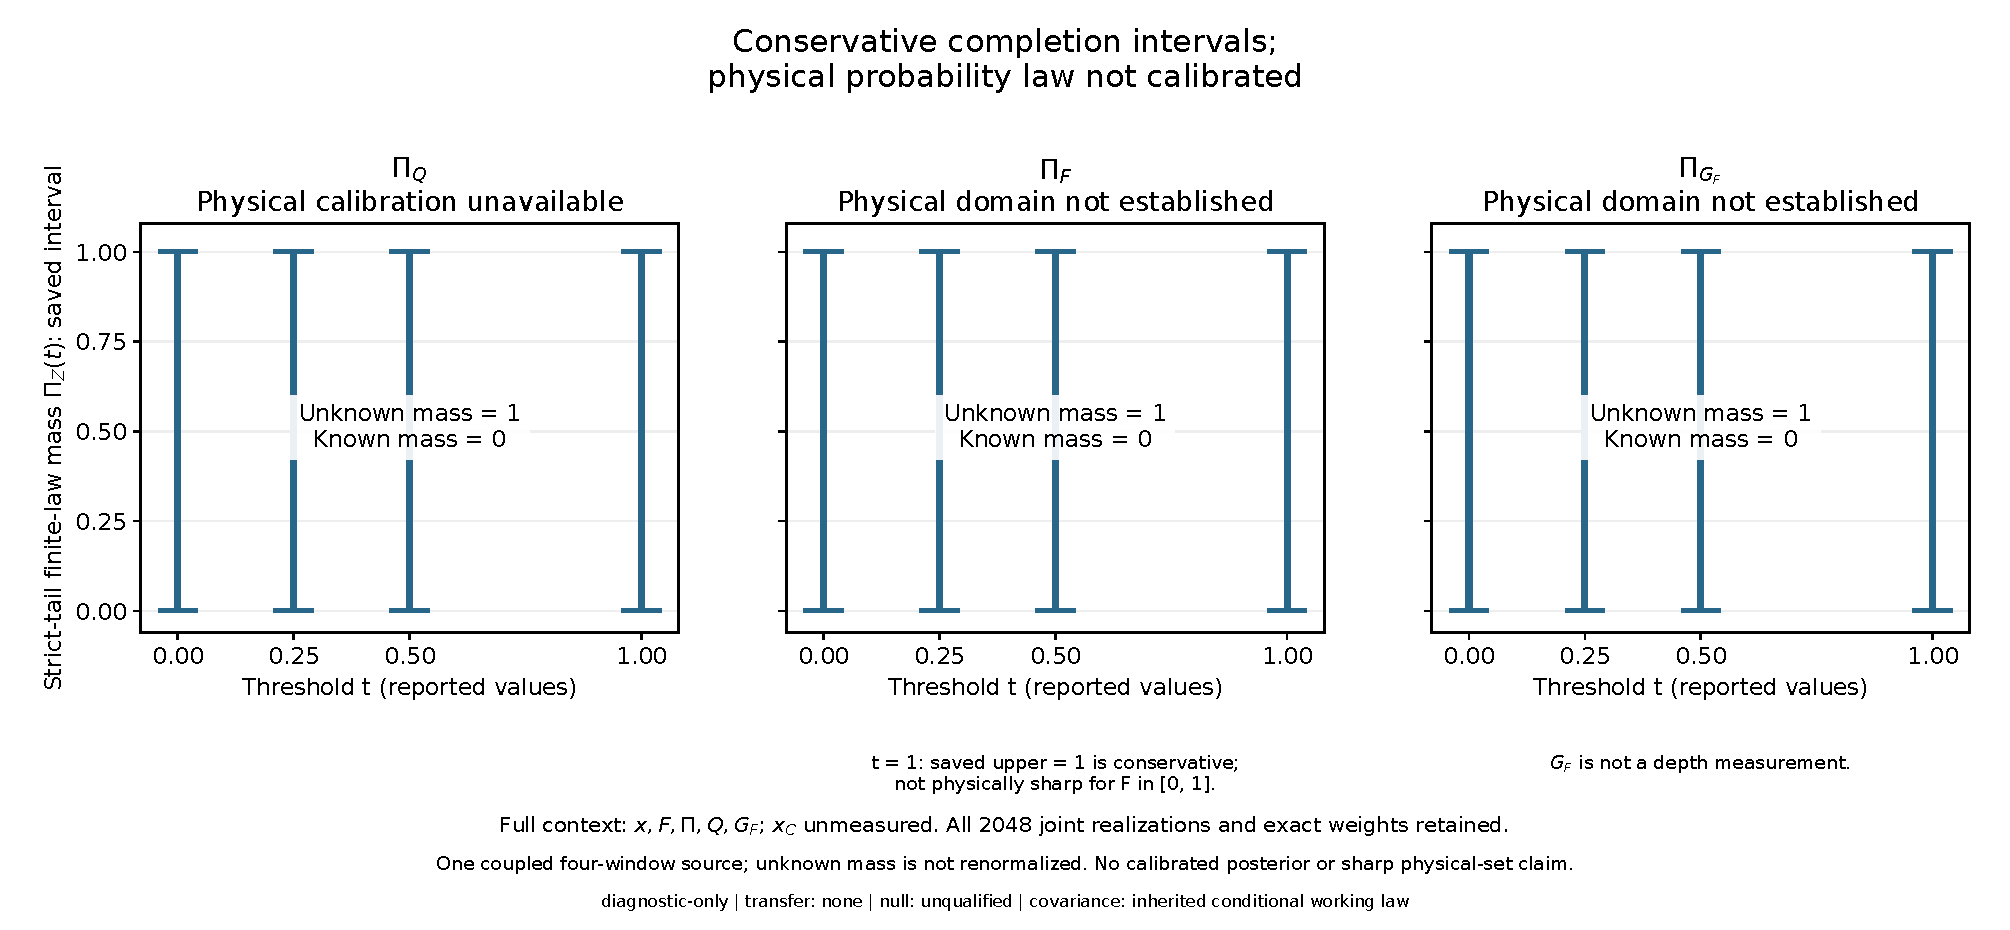
\includegraphics[width=\linewidth,height=.71\textheight,keepaspectratio]{figures/f001_external.pdf}
\caption{Conservative completion intervals for strict exceedance under the coupled 2048-point group-fit measure. Physical functions retain unknown mass one; their physical probability law is not calibrated. Zero, a threshold tie, and a function outside its domain are distinct. The displayed filling-fraction interval at threshold one is an outer completion envelope and is not asserted sharp.}
\label{fig:f001}
\end{figure}
\clearpage
\begin{figure}[p]
\centering
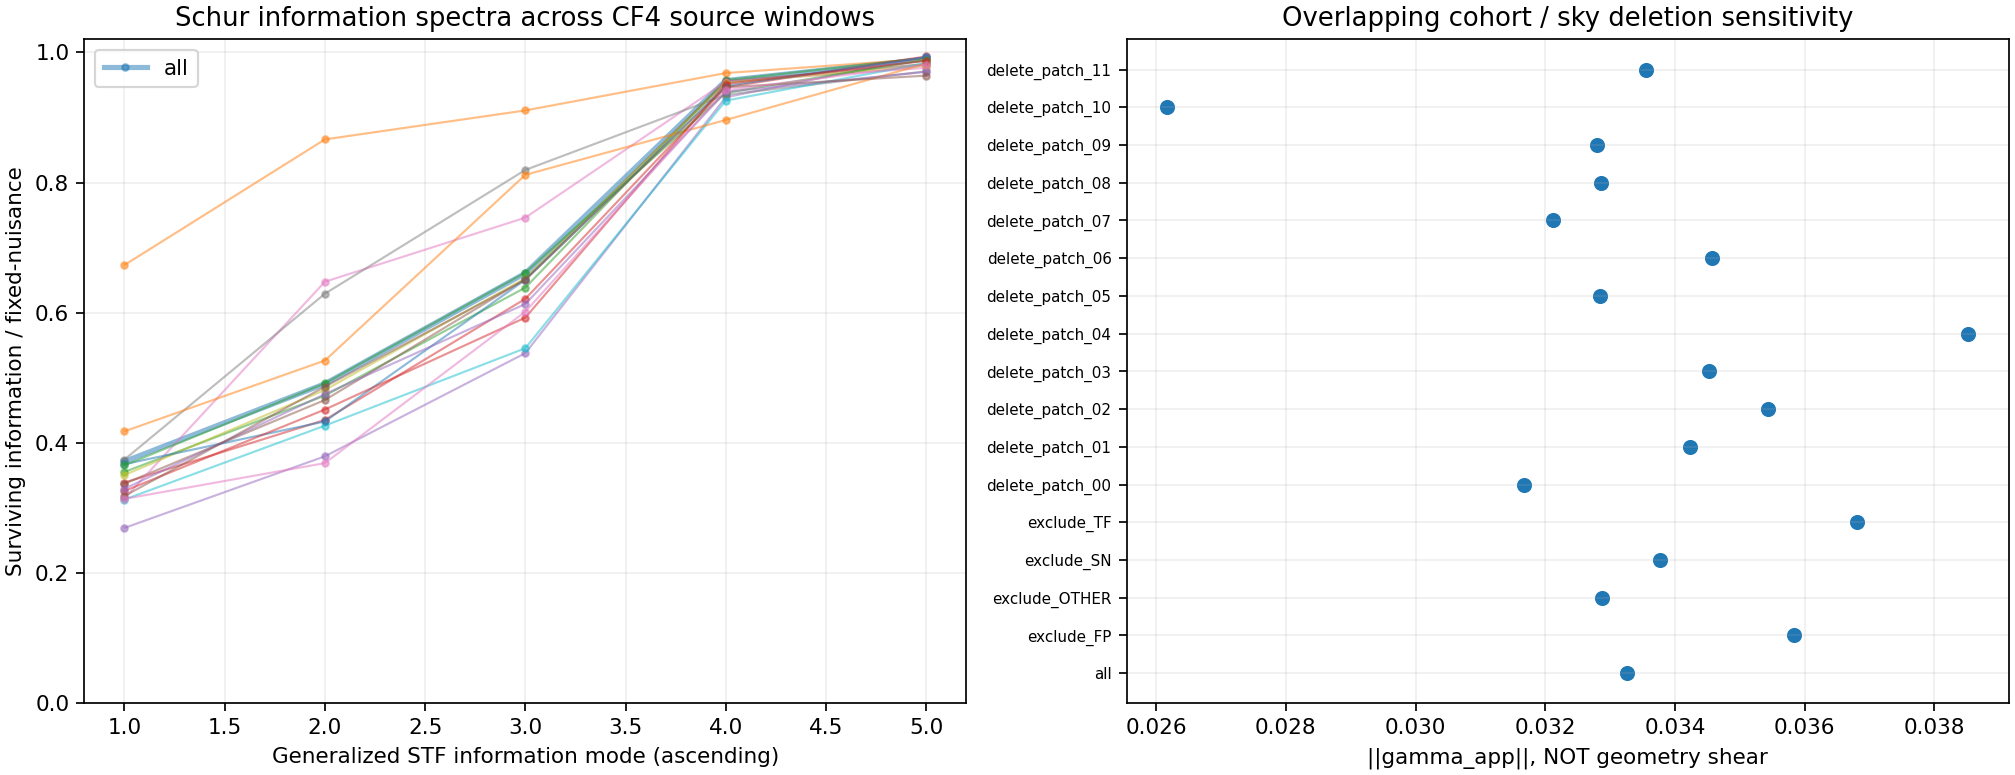
\includegraphics[width=\linewidth,height=.71\textheight,keepaspectratio]{figures/f002.png}
\caption{Conditional information for the full five-coordinate Cosmicflows STF response after nuisance profiling. Dependence assumptions change the retained information. The fit uses a fixed source-conditioned Gaussian design; these information and sensitivity summaries are not physical shear constraints.}
\label{fig:f002}
\end{figure}
\clearpage
\begin{figure}[p]
\centering
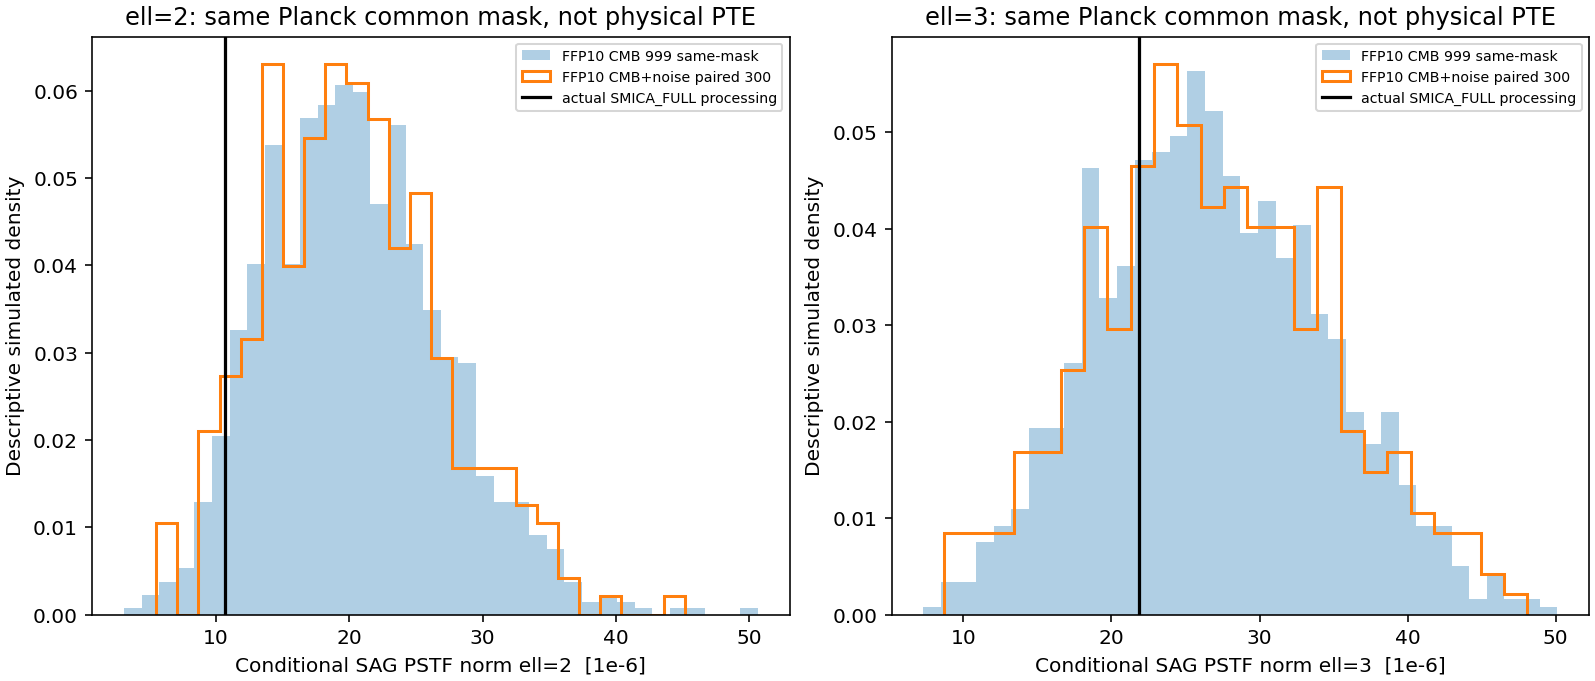
\includegraphics[width=\linewidth,height=.71\textheight,keepaspectratio]{figures/f004.png}
\caption{Low-multipole normalization and mask effects in retained Planck source simulations. The angular moments and finite mask response are evaluated with their stated tensor convention. One observed sky and fixed-weight simulations do not supply the all-observer derivative assumptions required for a physical near-isotropy bound.}
\label{fig:f004}
\end{figure}
\clearpage
\begin{figure}[p]
\centering
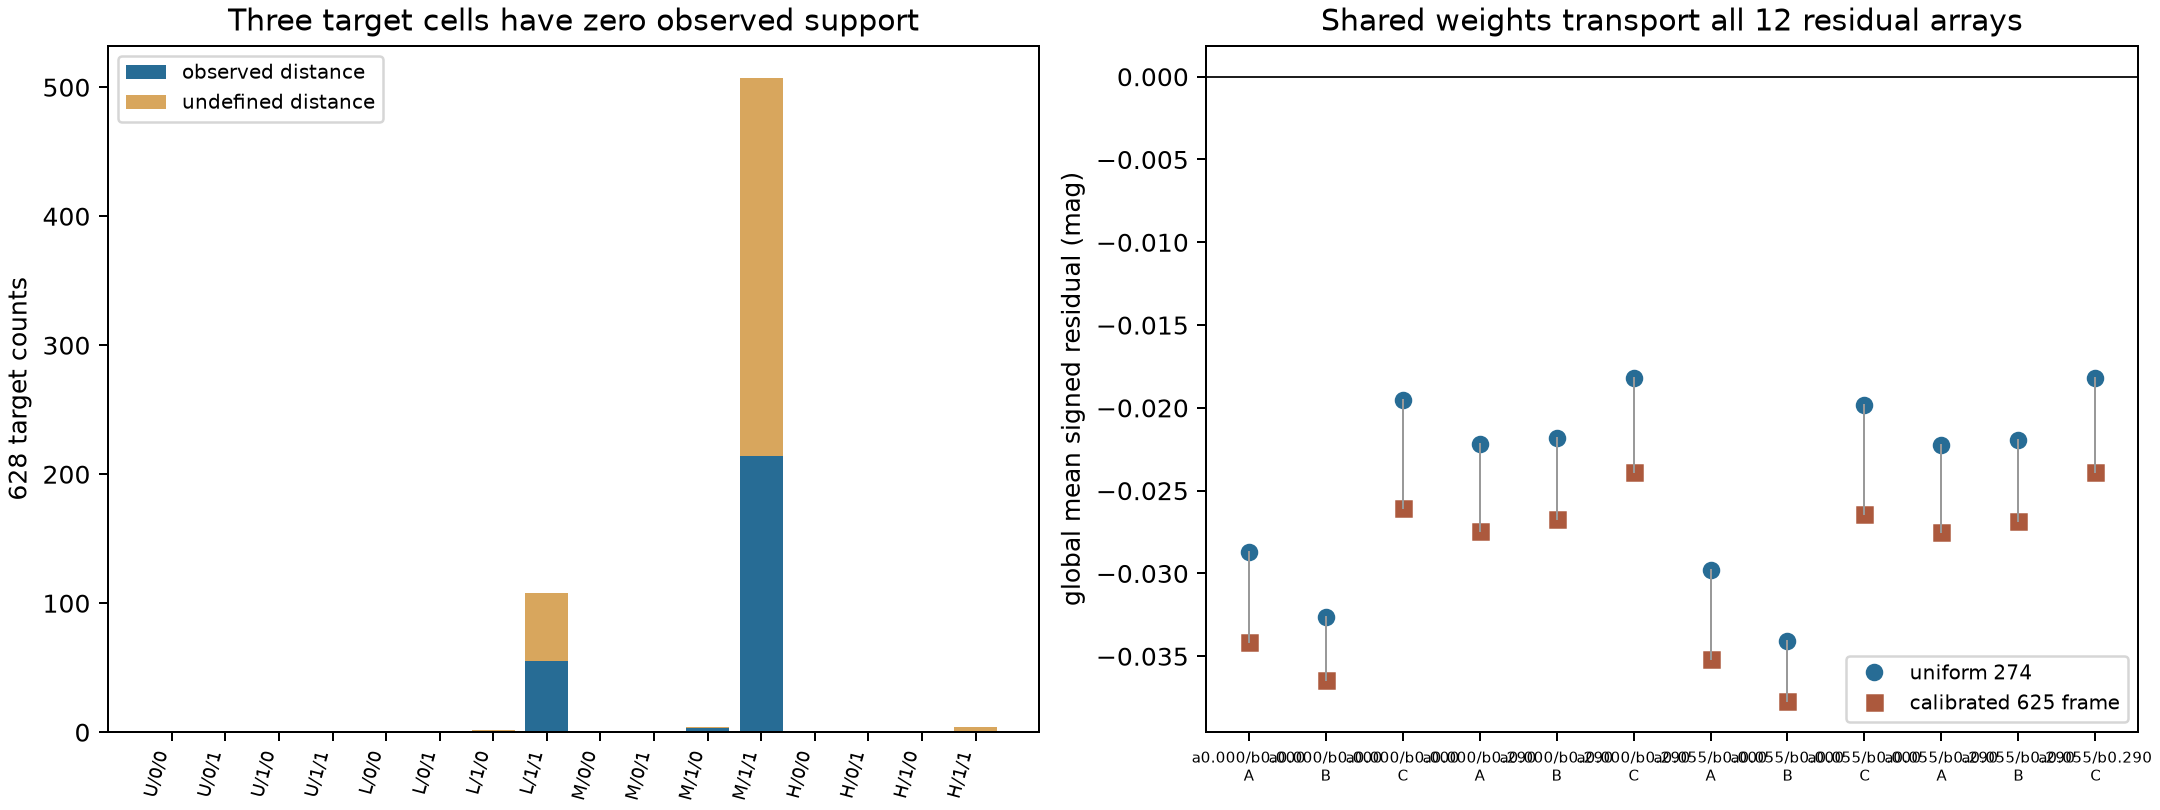
\includegraphics[width=\linewidth,height=.71\textheight,keepaspectratio]{figures/f005.png}
\caption{Auxiliary support and calibrated residual means in the incomplete distance cohort. Unsupported cells prevent exact balancing of the full target frame. Removing them changes the target; positive weights in the restricted frame do not identify missing outcomes or a physical selected-source law.}
\label{fig:f005}
\end{figure}
\clearpage
\begin{figure}[p]
\centering
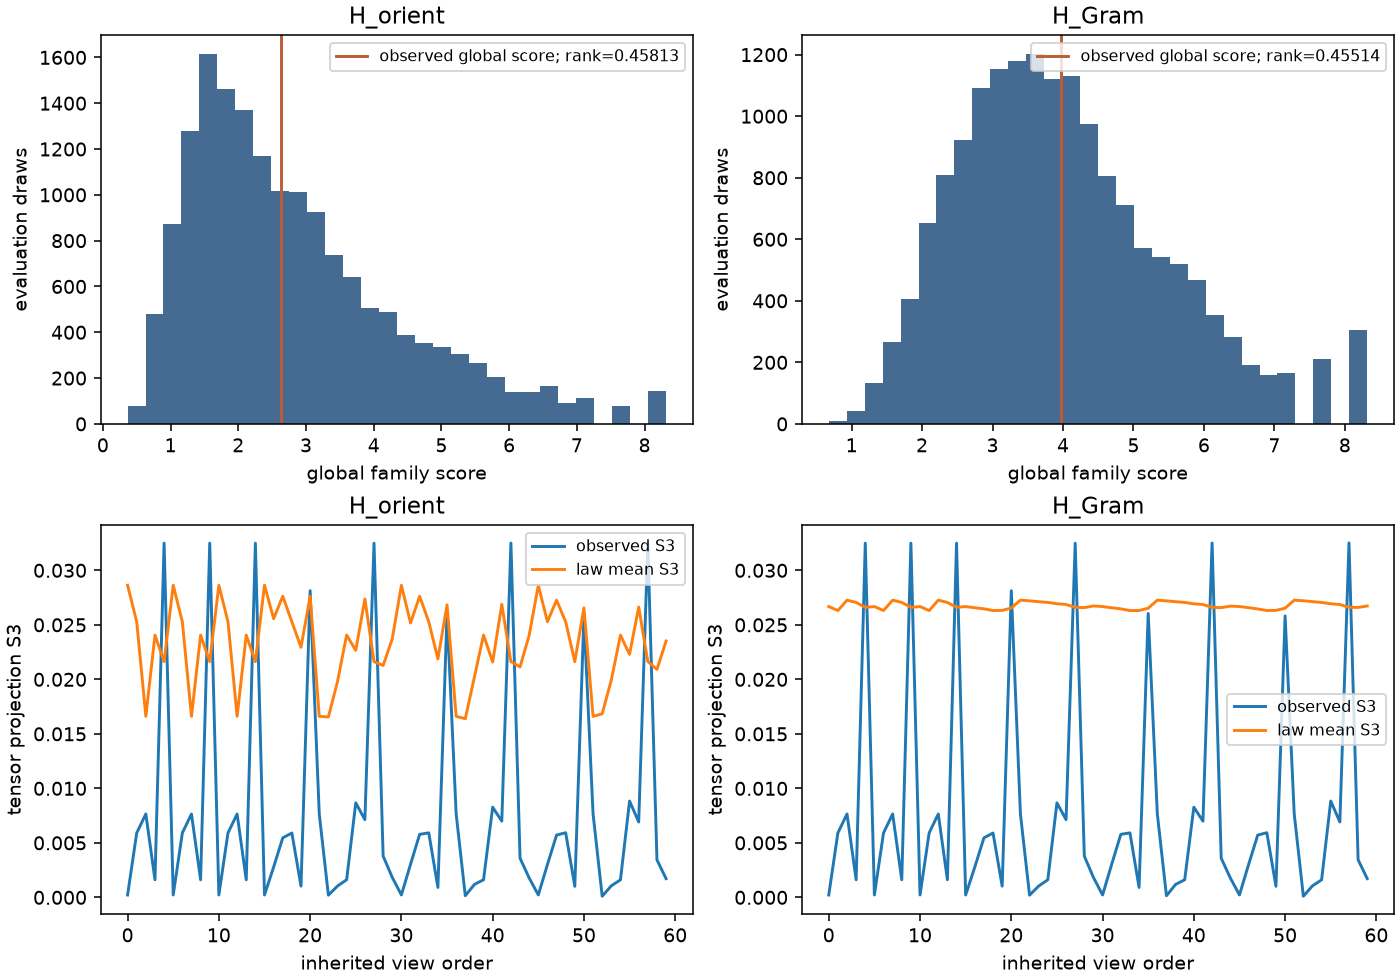
\includegraphics[width=\linewidth,height=.71\textheight,keepaspectratio]{figures/f008.png}
\caption{Constructed spatial-rotation and Gram-preserving reference laws for sixty processed E-pseudoalm views of one Planck sky. A common action preserves dependence across views. The ranks and Monte Carlo intervals refer to the named conditional laws; actual mask and foreground invariance is not established.}
\label{fig:f008}
\end{figure}
\clearpage
\begin{figure}[p]
\centering
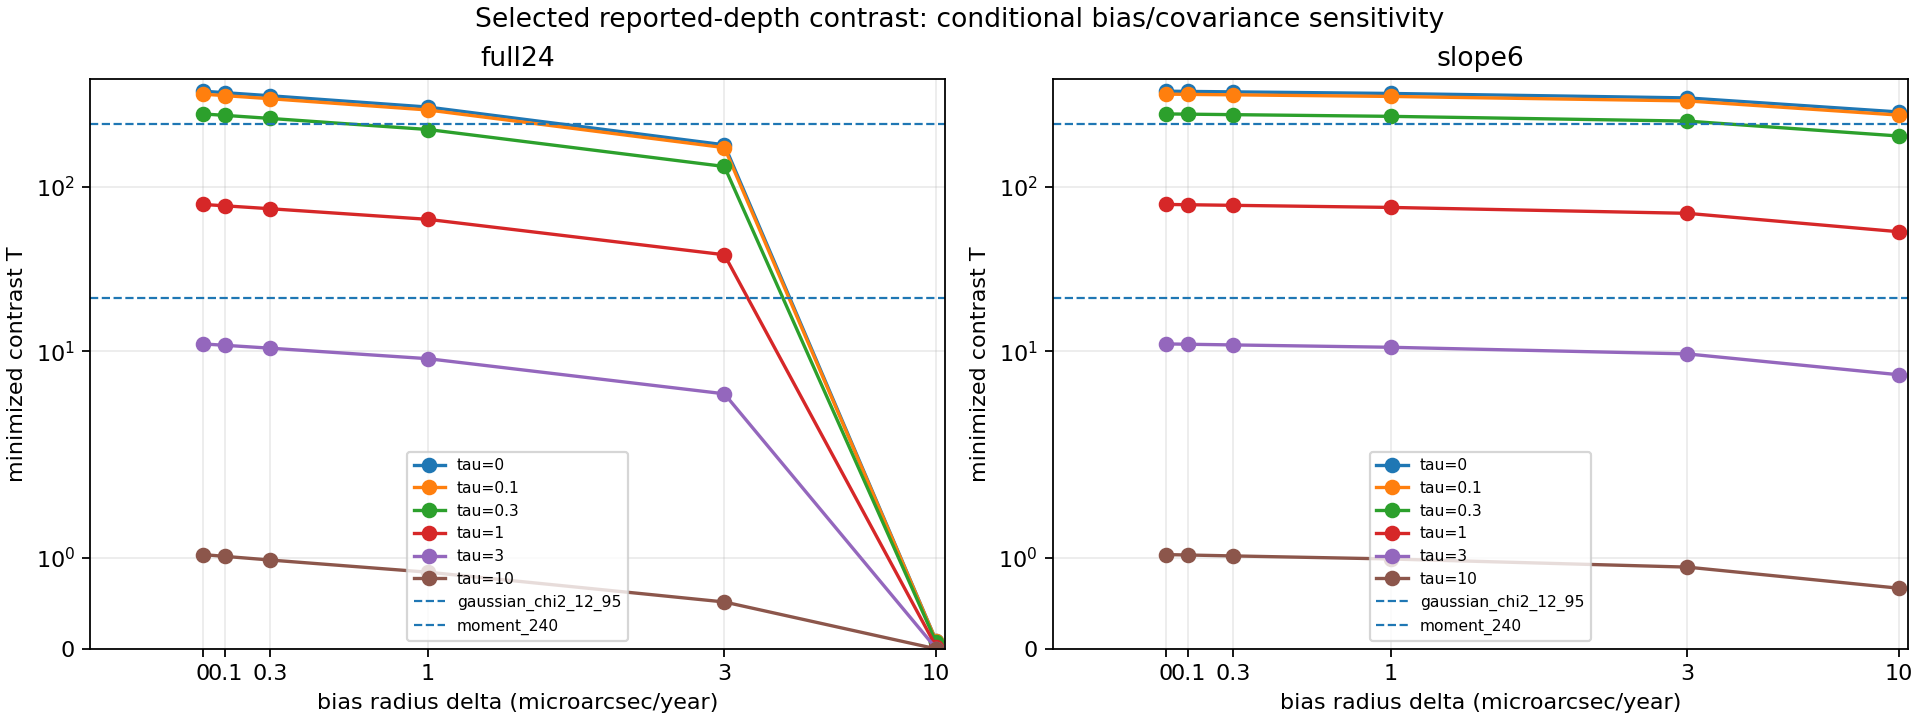
\includegraphics[width=\linewidth,height=.71\textheight,keepaspectratio]{figures/f009.png}
\caption{Conditional reported-depth bias frontier for the full astrometric state and the slope-restricted subspace. Each curve minimizes the contrast quadratic over the stated bias ball with all covariance cross blocks retained. The radii are scenarios, not measured Gaia biases or calibrated physical exclusions.}
\label{fig:f009}
\end{figure}
\clearpage
\begin{figure}[p]
\centering
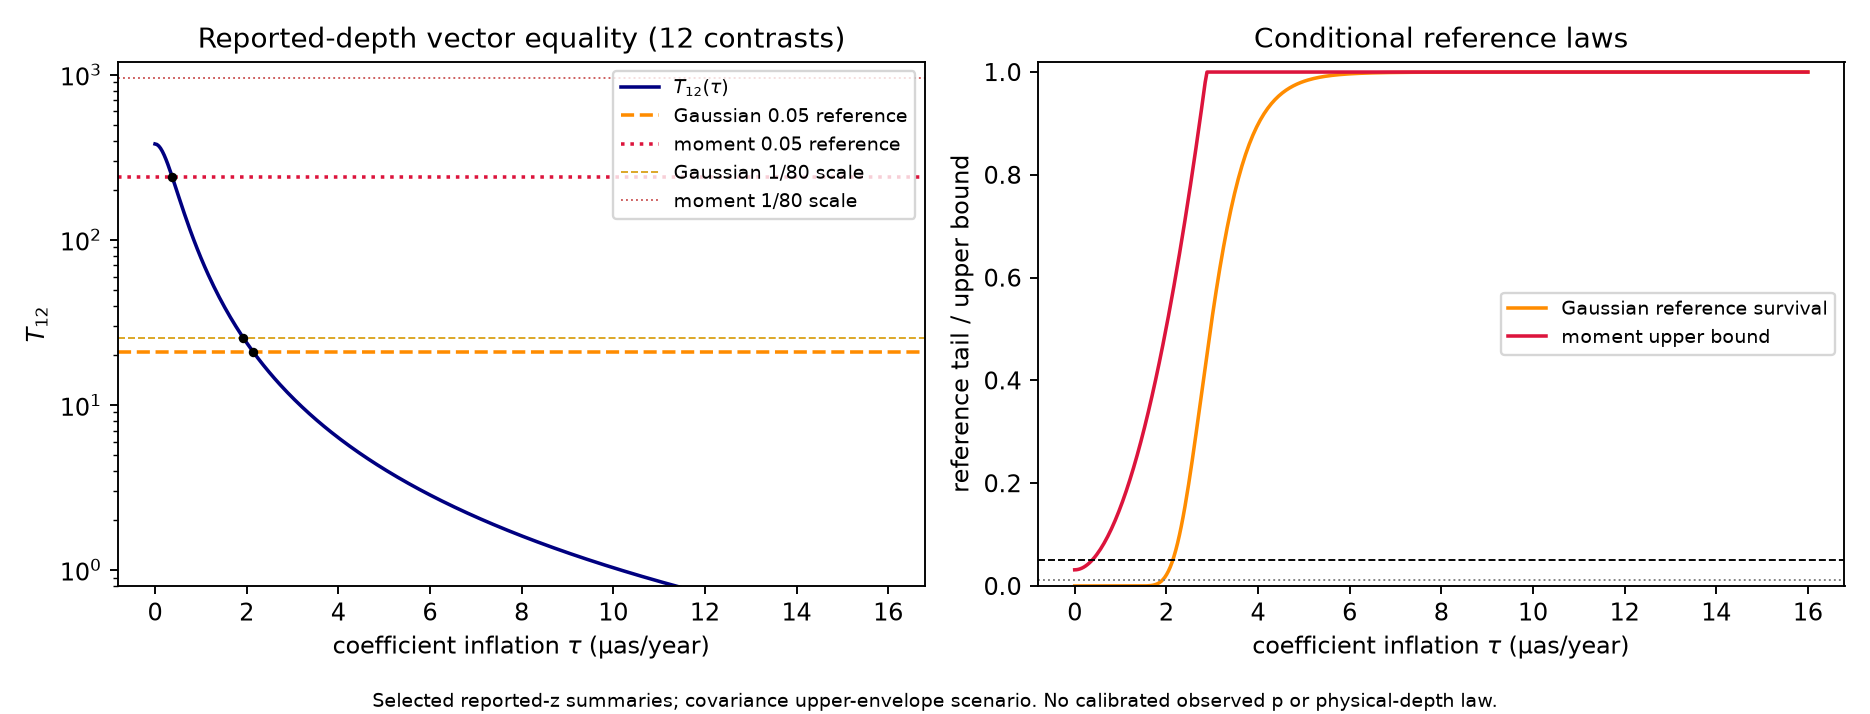
\includegraphics[width=\linewidth,height=.71\textheight,keepaspectratio]{figures/f010.png}
\caption{Reported-depth constancy under covariance inflation. The Gaussian and distribution-free moment lines require their respective mean and covariance-domination assumptions. The actual cross-source covariance is unknown, so the plotted tails and crossings are conditional sensitivity results.}
\label{fig:f010}
\end{figure}
\clearpage
\begin{figure}[p]
\centering
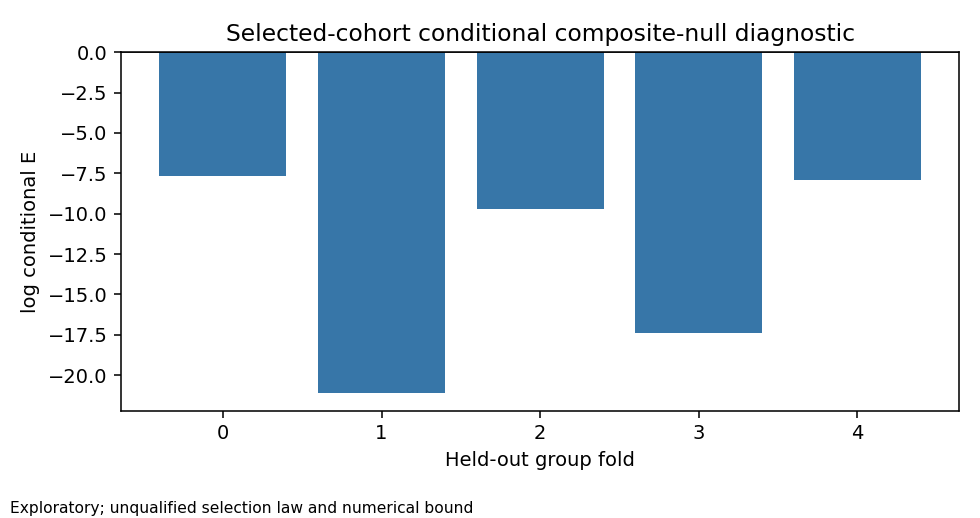
\includegraphics[width=\linewidth,height=.71\textheight,keepaspectratio]{figures/f011.png}
\caption{Conditional distance-model ratios on whole-group held-out blocks. The fixed normalized alternative mixture is compared with a composite null; dependent fold ratios are averaged rather than multiplied. Selection, adaptive choices, and numerical null-supremum qualification prevent interpreting these values as calibrated observational evidence.}
\label{fig:f011}
\end{figure}
\clearpage
\begin{figure}[p]
\centering
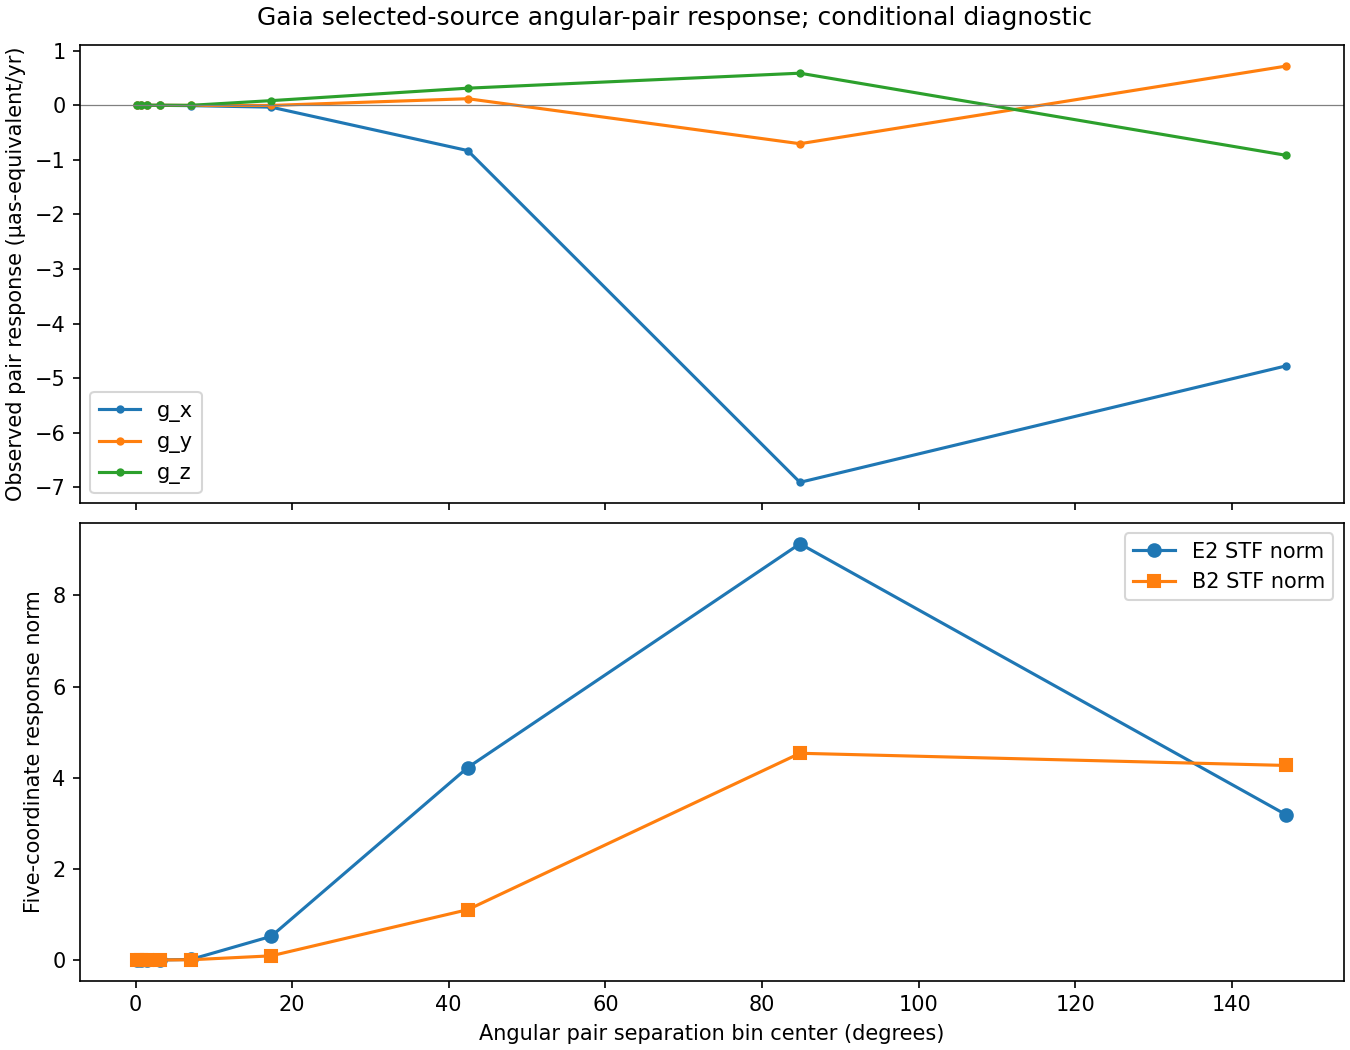
\includegraphics[width=\linewidth,height=.71\textheight,keepaspectratio]{figures/f012.png}
\caption{Angular-pair responses and representative vector/STF profiles for the retained Gaia source set. The measured response is the binned operator applied to tangent motions, not a coefficient estimate. Shared-source covariance is included; cross-source covariance and source-selection calibration are unavailable. Angular separation is not depth.}
\label{fig:f012}
\end{figure}
\clearpage
\begin{figure}[p]
\centering
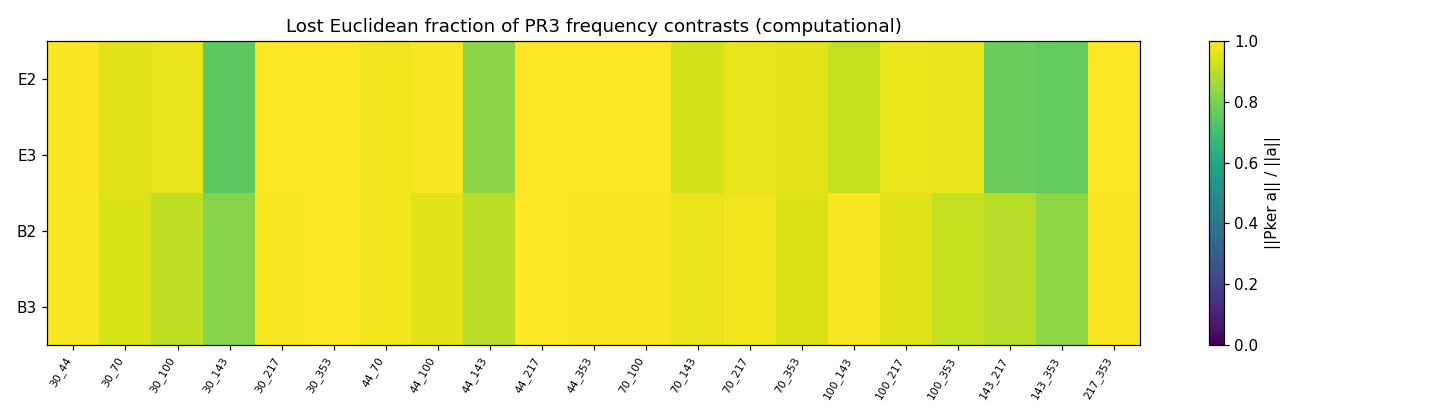
\includegraphics[width=\linewidth,height=.71\textheight,keepaspectratio]{figures/f013.png}
\caption{Spectral information lost by a single cleaned CMB map. The finite seven-channel linear compression maps 168 real harmonic coordinates to 24, with rank 24 and a 144-dimensional kernel. Frequency contrasts can lie in that kernel. This is a response-space calculation for the retained weights, not a seven-frequency sky measurement or a foreground rejection.}
\label{fig:f013}
\end{figure}
\clearpage
\begin{figure}[p]
\centering
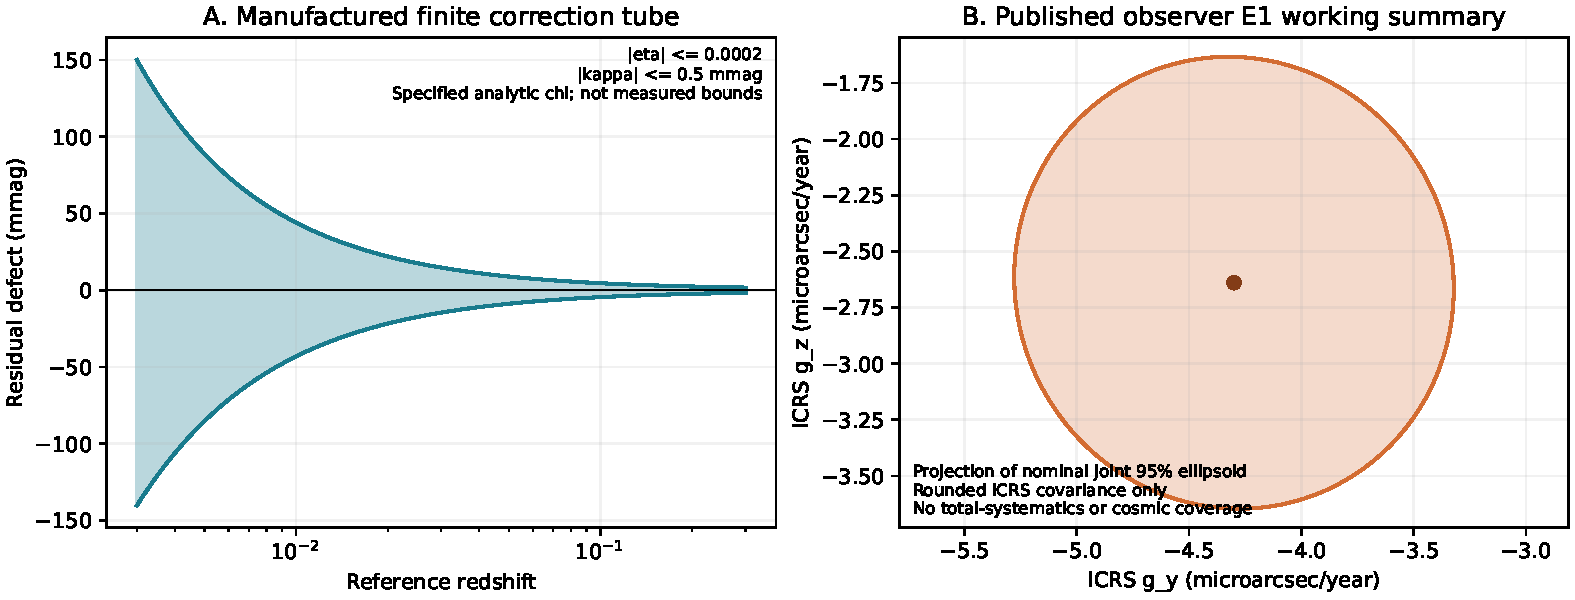
\includegraphics[width=\linewidth,height=.71\textheight,keepaspectratio]{figures/f014.pdf}
\caption{Conditional analytic and observational response comparisons. The finite response example uses declared nuisance radii; the astrometric panel uses its published observer-vector working summary. Neither an assumed radius nor an observer pattern is a measured bound on a cosmological history.}
\label{fig:f014}
\end{figure}
\clearpage
\begin{figure}[p]
\centering
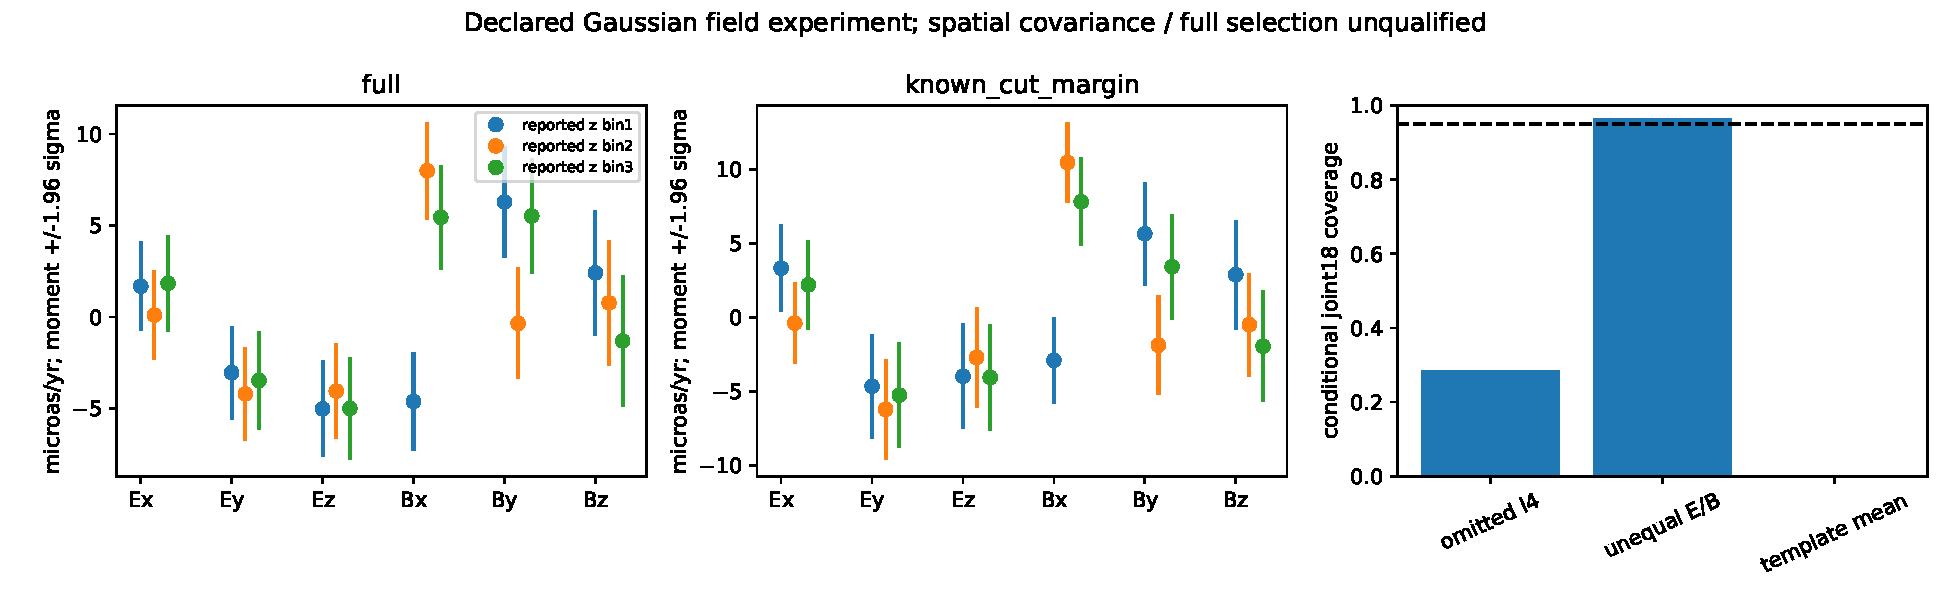
\includegraphics[width=\linewidth,height=.71\textheight,keepaspectratio]{figures/f015_external.pdf}
\caption{Reported-redshift astrometric vectors and simulated joint-coverage checks. The error bars use the stated working source covariance. Omitted high-order angular structure and template-correlated means can invalidate that coverage. Spatial covariance, full selection, true-depth response, and physical source motion remain unqualified.}
\label{fig:f015}
\end{figure}
\clearpage
\begin{figure}[p]
\centering
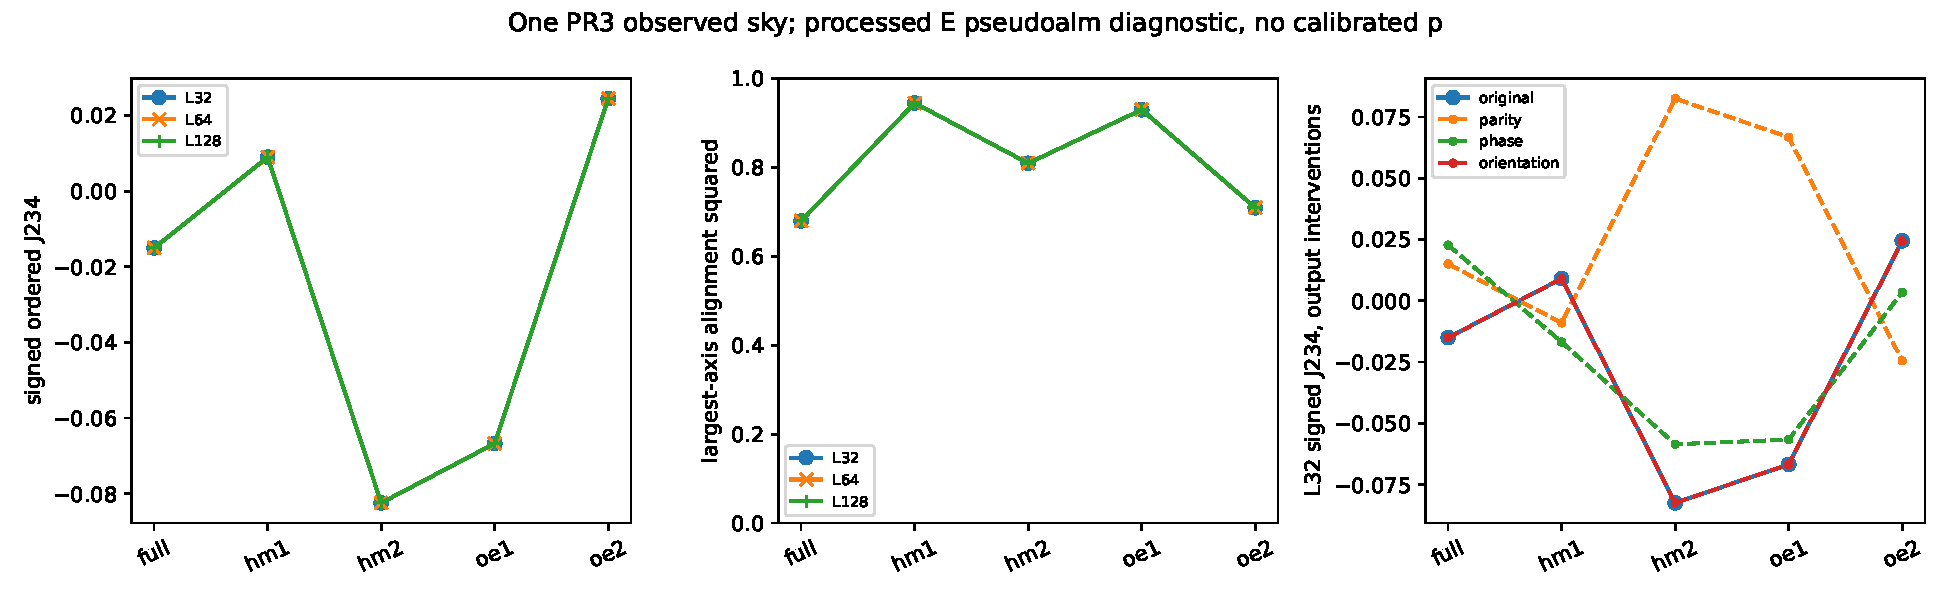
\includegraphics[width=\linewidth,height=.71\textheight,keepaspectratio]{figures/f016.pdf}
\caption{Counterpairs of processed Planck E morphology with signed contraction and axis summaries. These interventions on one observed sky demonstrate that the chosen summaries retain different information. They are retrospective processing comparisons without a calibrated physical null.}
\label{fig:f016}
\end{figure}
\clearpage
\begin{figure}[p]
\centering
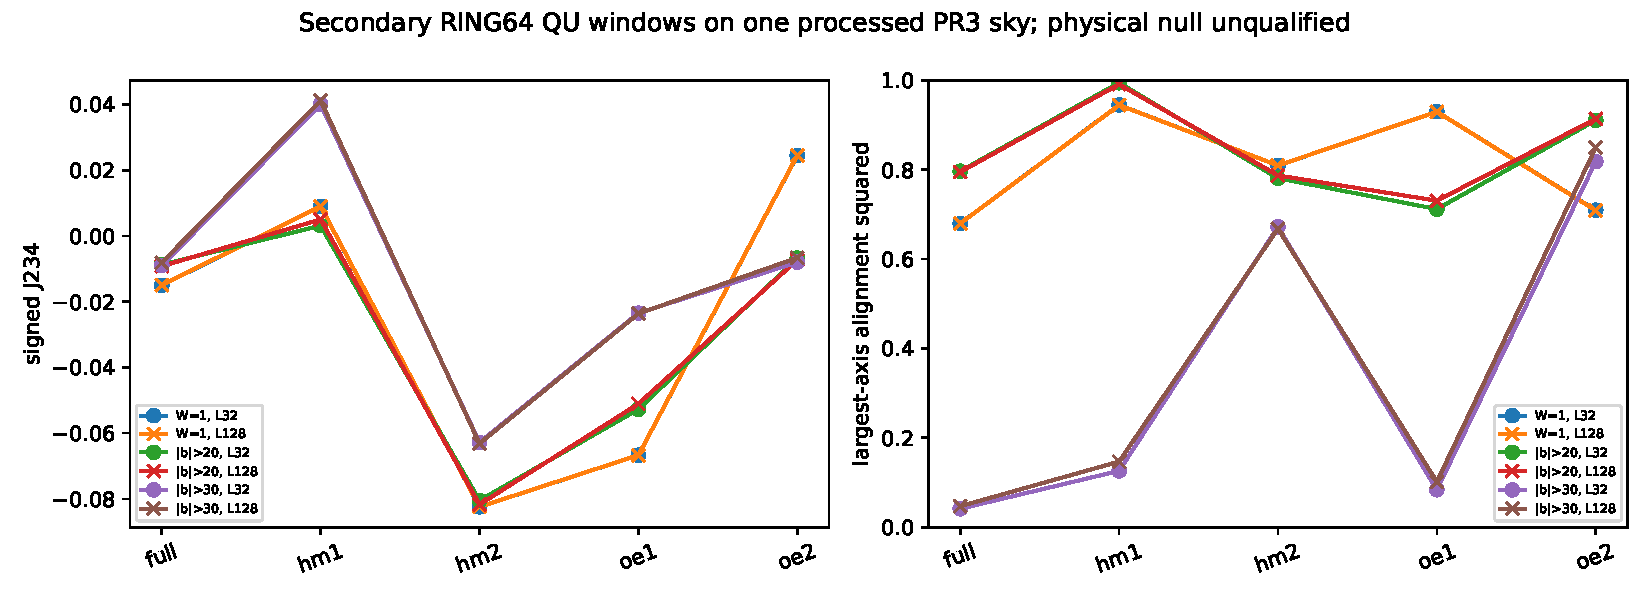
\includegraphics[width=\linewidth,height=.71\textheight,keepaspectratio]{figures/f017_external.pdf}
\caption{Secondary selected-sky windows applied to delivered Planck Q/U on one processed sky. Changes in the signed descriptor and axis alignment expose processing dependence. The windows and multipole cutoffs do not form independent sky realizations, and the physical total-field null is not calibrated.}
\label{fig:f017}
\end{figure}
\clearpage
\begin{figure}[p]
\centering
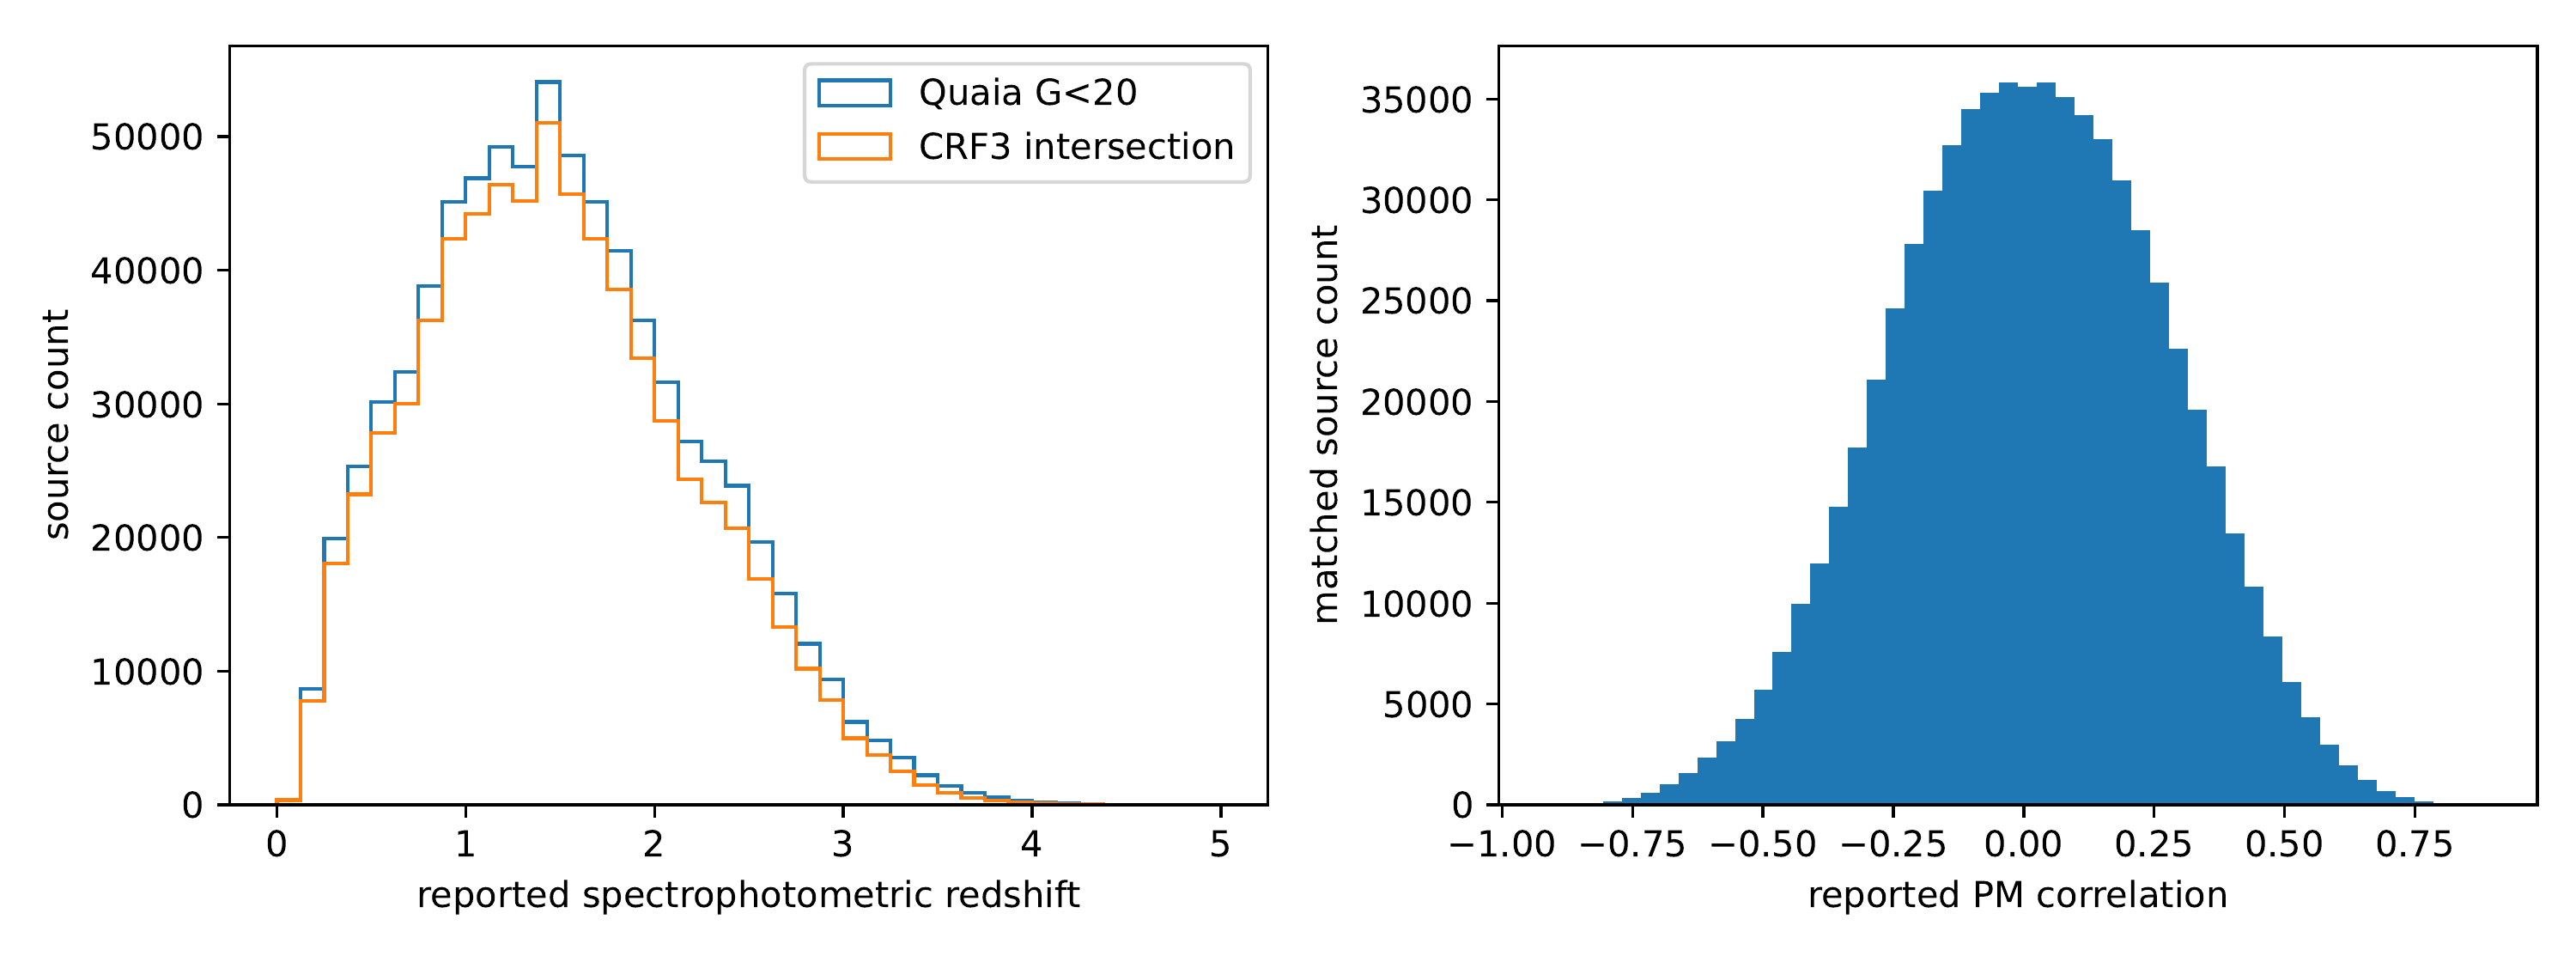
\includegraphics[width=\linewidth,height=.71\textheight,keepaspectratio]{figures/f018_external.png}
\caption{Exact-identity linkage of the selected Quaia and Gaia samples before the later supplement. The displayed redshift and match distributions describe catalogue membership. They do not measure acceleration, certify true distances, or supply a centroid-to-matter response.}
\label{fig:f018}
\end{figure}
\clearpage
\begin{figure}[p]
\centering
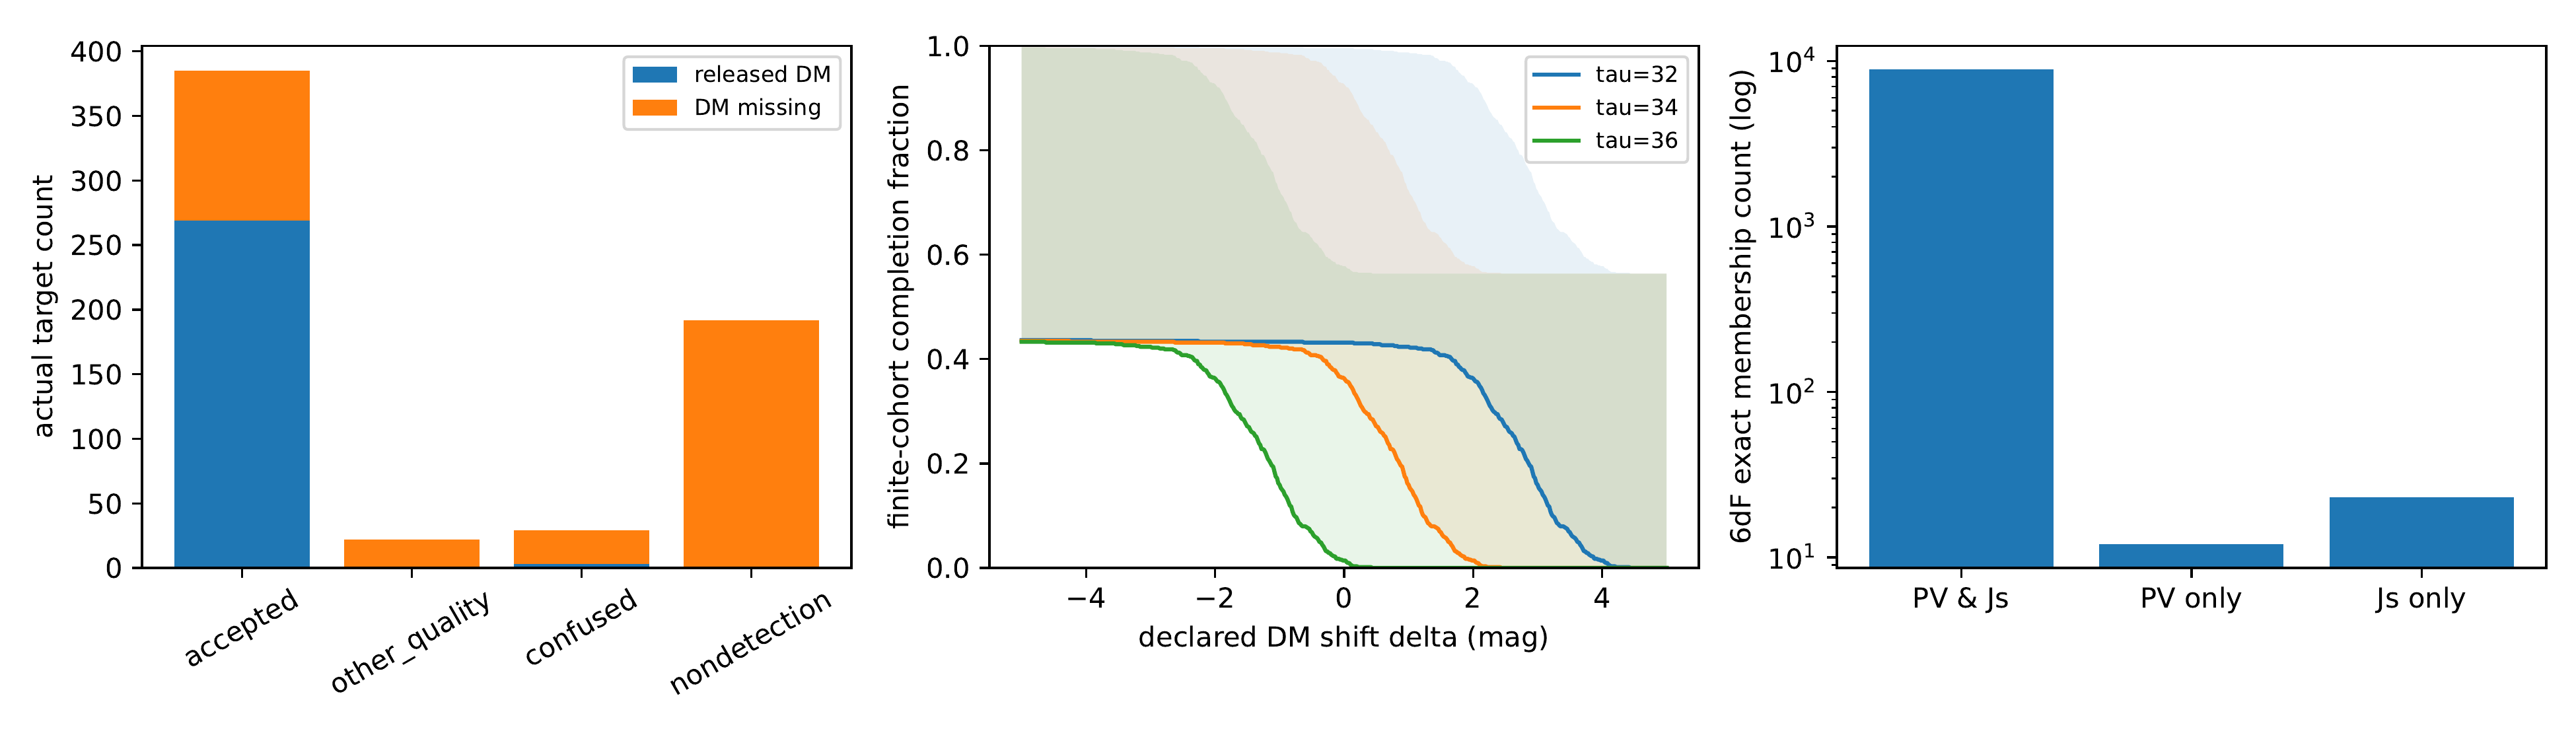
\includegraphics[width=\linewidth,height=.71\textheight,keepaspectratio]{figures/f019_external.png}
\caption{Observed outcome marks and declared missing-modulus completions in the selected distance cohort. The completion curves are conditional sensitivity models. They do not estimate the parent inclusion probability or establish the physical law of missing outcomes.}
\label{fig:f019}
\end{figure}
\clearpage
\begin{figure}[p]
\centering
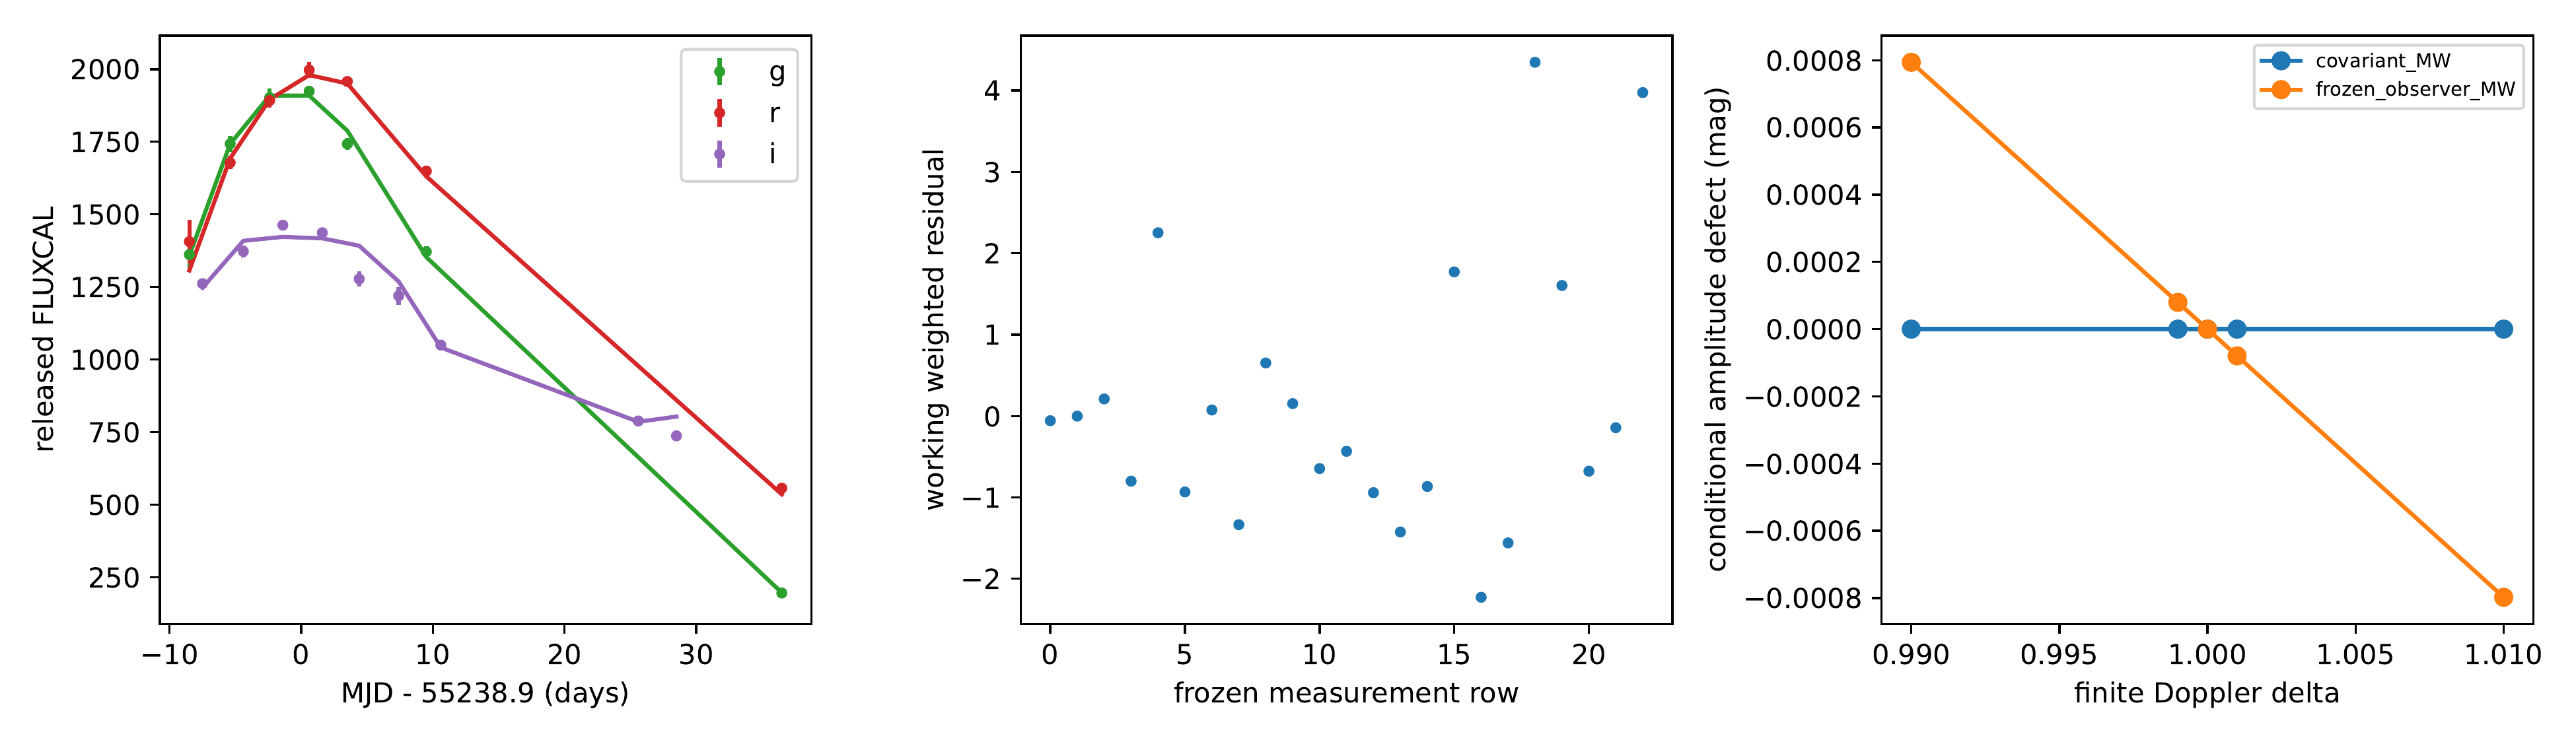
\includegraphics[width=\linewidth,height=.71\textheight,keepaspectratio]{figures/f020_external.png}
\caption{The retained SN010010 light curve, measurement-only residuals, and conditional amplitude response. The baseline fails its stated adequacy screen, and the nominal producer fit is not reproduced. This earlier diagnostic is retained to show the actual failure; the later public model-covariance calculation addresses a different question.}
\label{fig:f020}
\end{figure}
\clearpage
\begin{figure}[p]
\centering
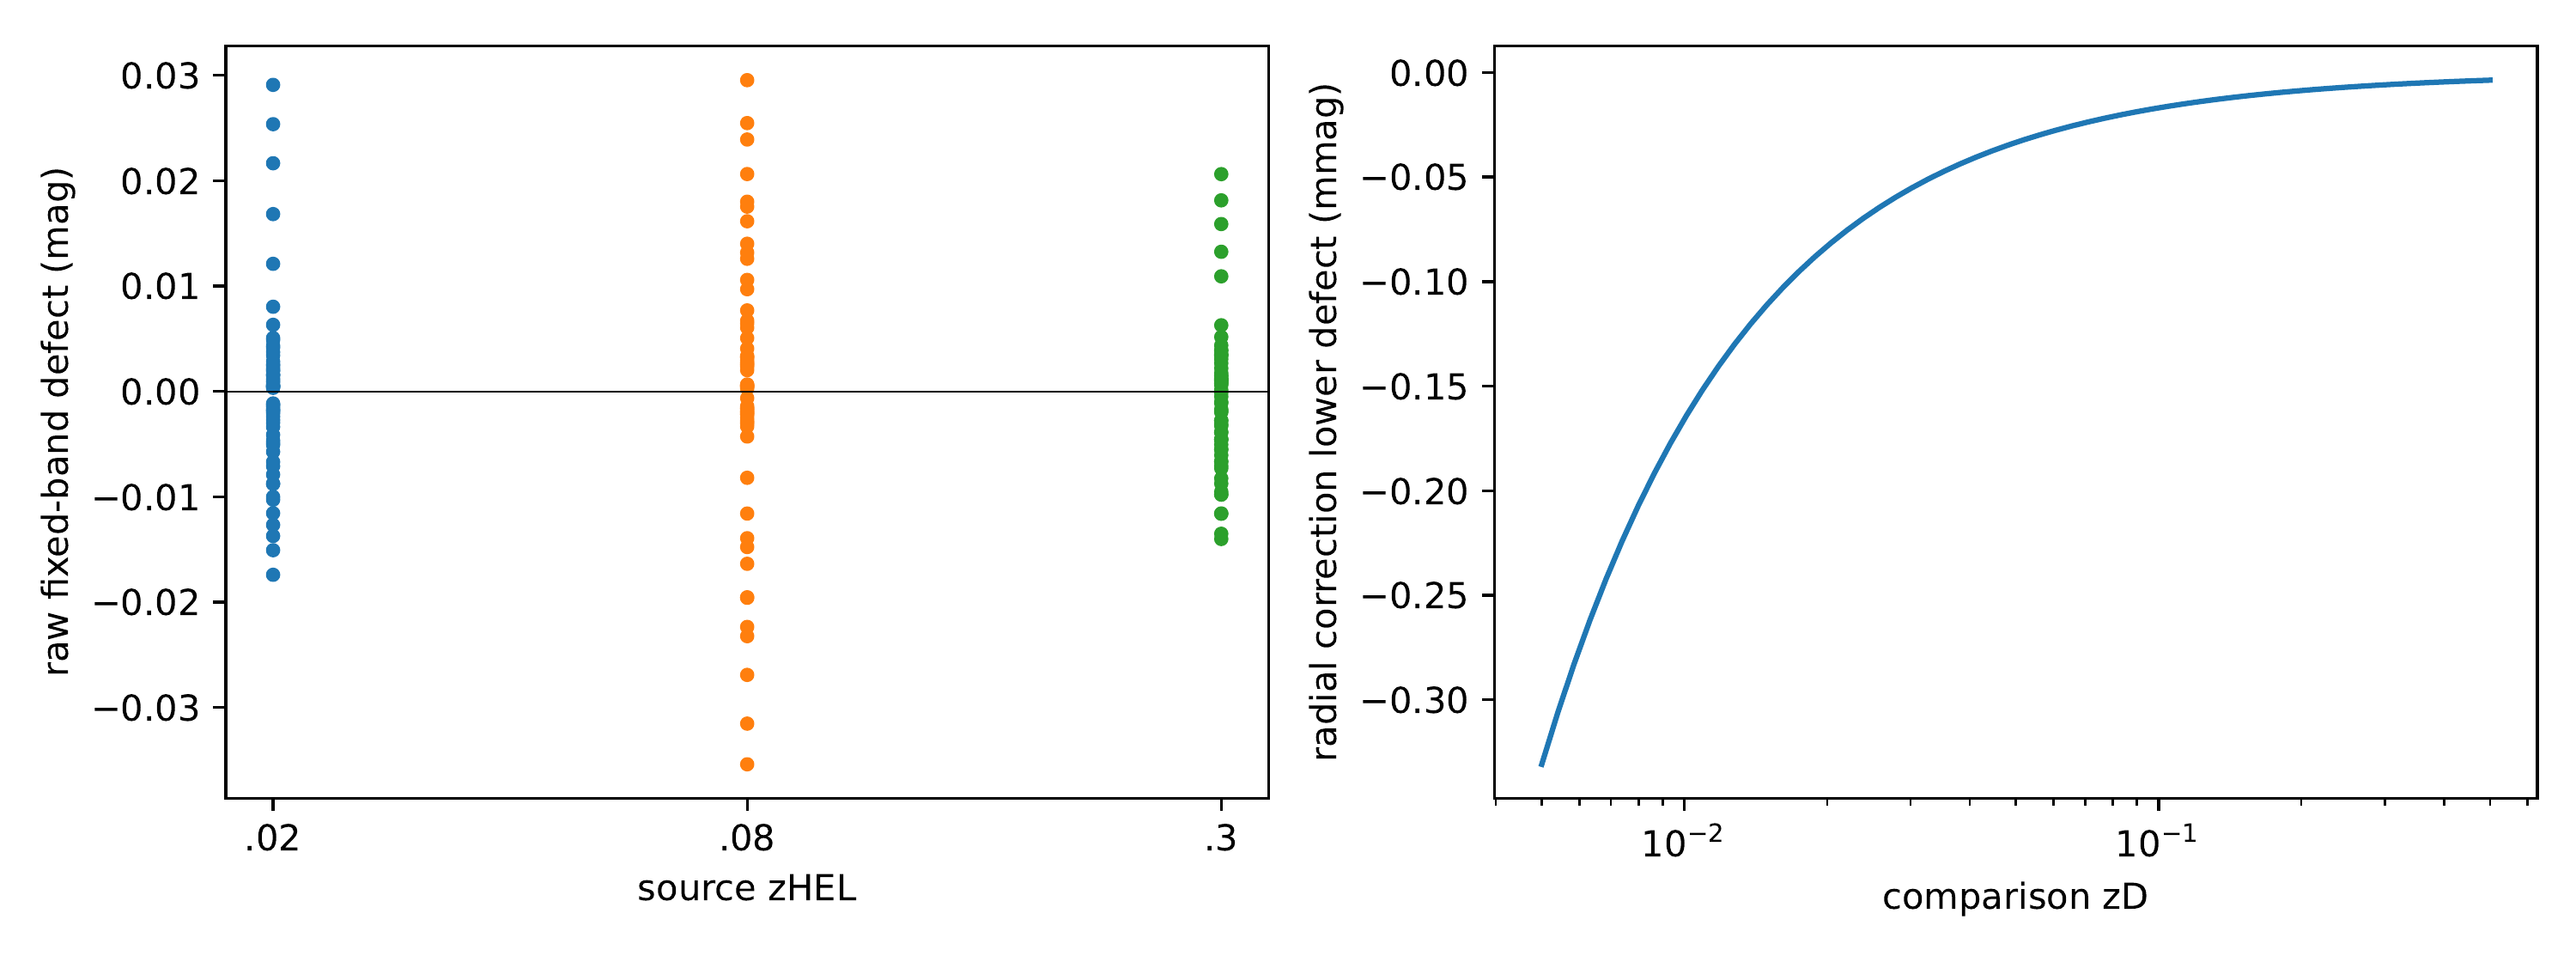
\includegraphics[width=\linewidth,height=.71\textheight,keepaspectratio]{figures/f021_external.png}
\caption{Finite spectral-refit and conditional radial-correction responses at separately specified source redshifts. A finite source calculation is not an empirical total observer-reboost correction. The nominal fitting, calibration, selection, and physical propagation responses remain additional inputs.}
\label{fig:f021}
\end{figure}
\clearpage
\begin{figure}[p]
\centering
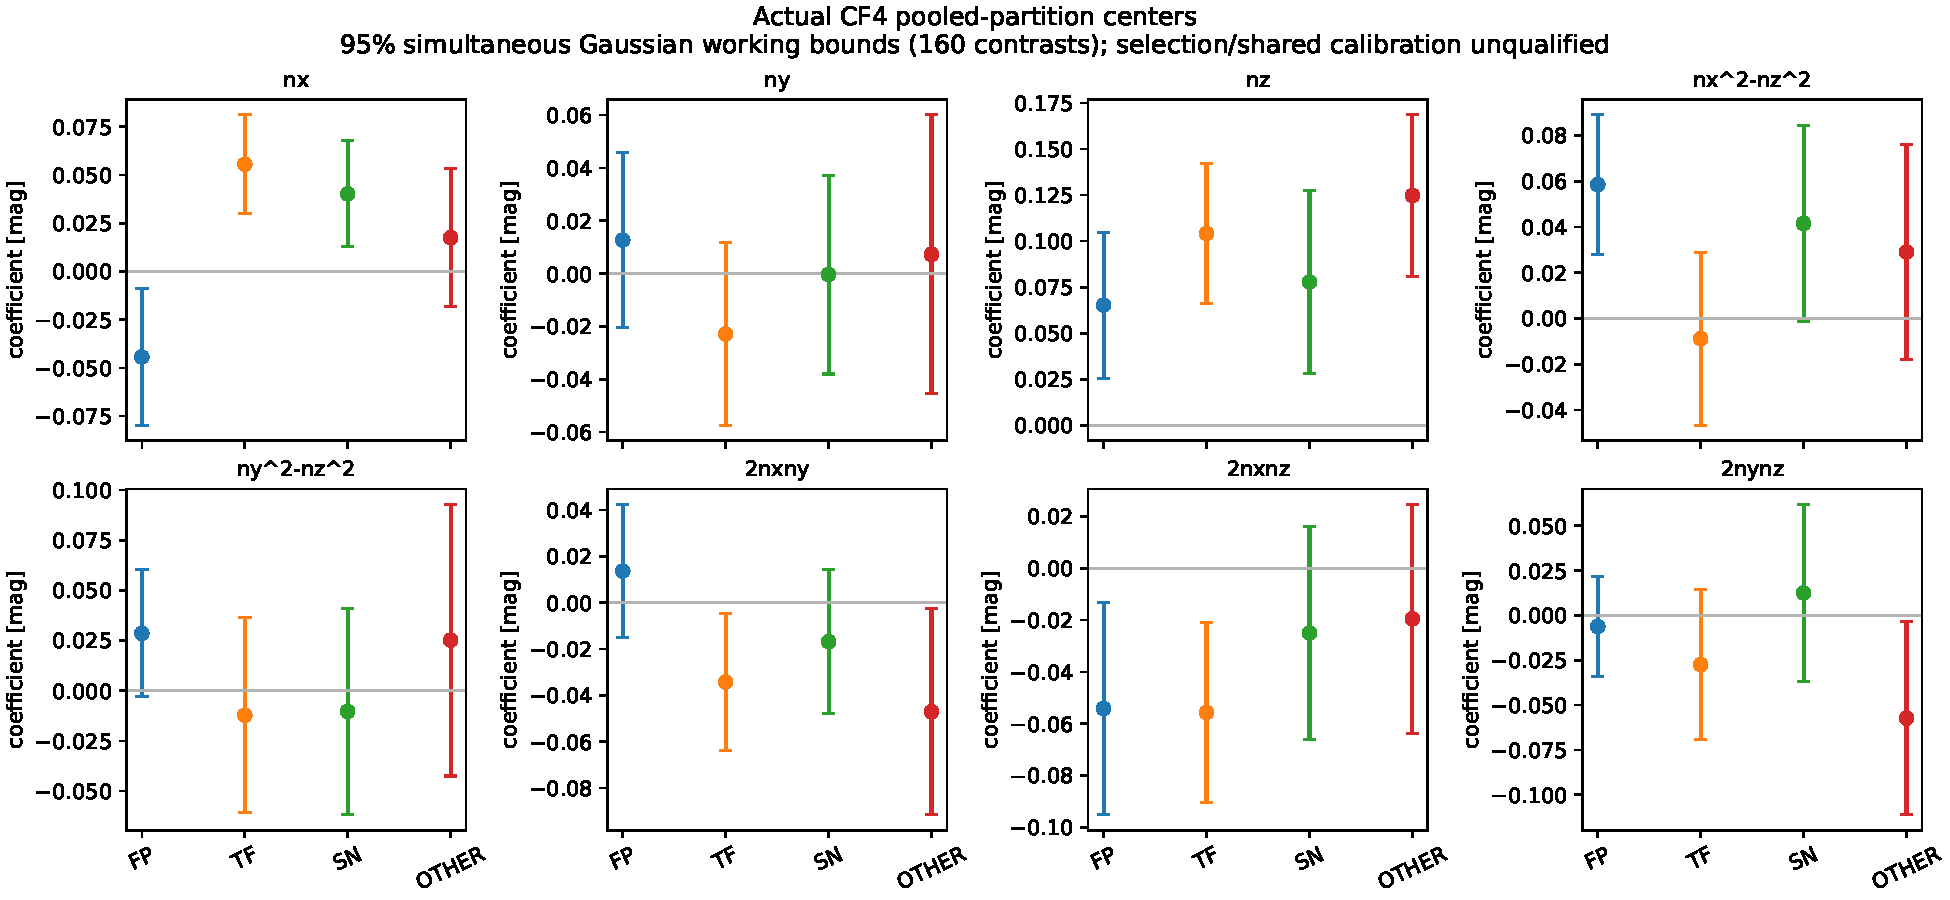
\includegraphics[width=\linewidth,height=.71\textheight,keepaspectratio]{figures/f022_external.pdf}
\caption{Observed method-dependent calibration contrasts on the retained Cosmicflows group geometry. These fitted centres supplement radius-only sensitivity calculations. Shared sources and calibration gauges remain, so method columns cannot be treated as independent physical measurements.}
\label{fig:f022}
\end{figure}
\clearpage
\begin{figure}[p]
\centering
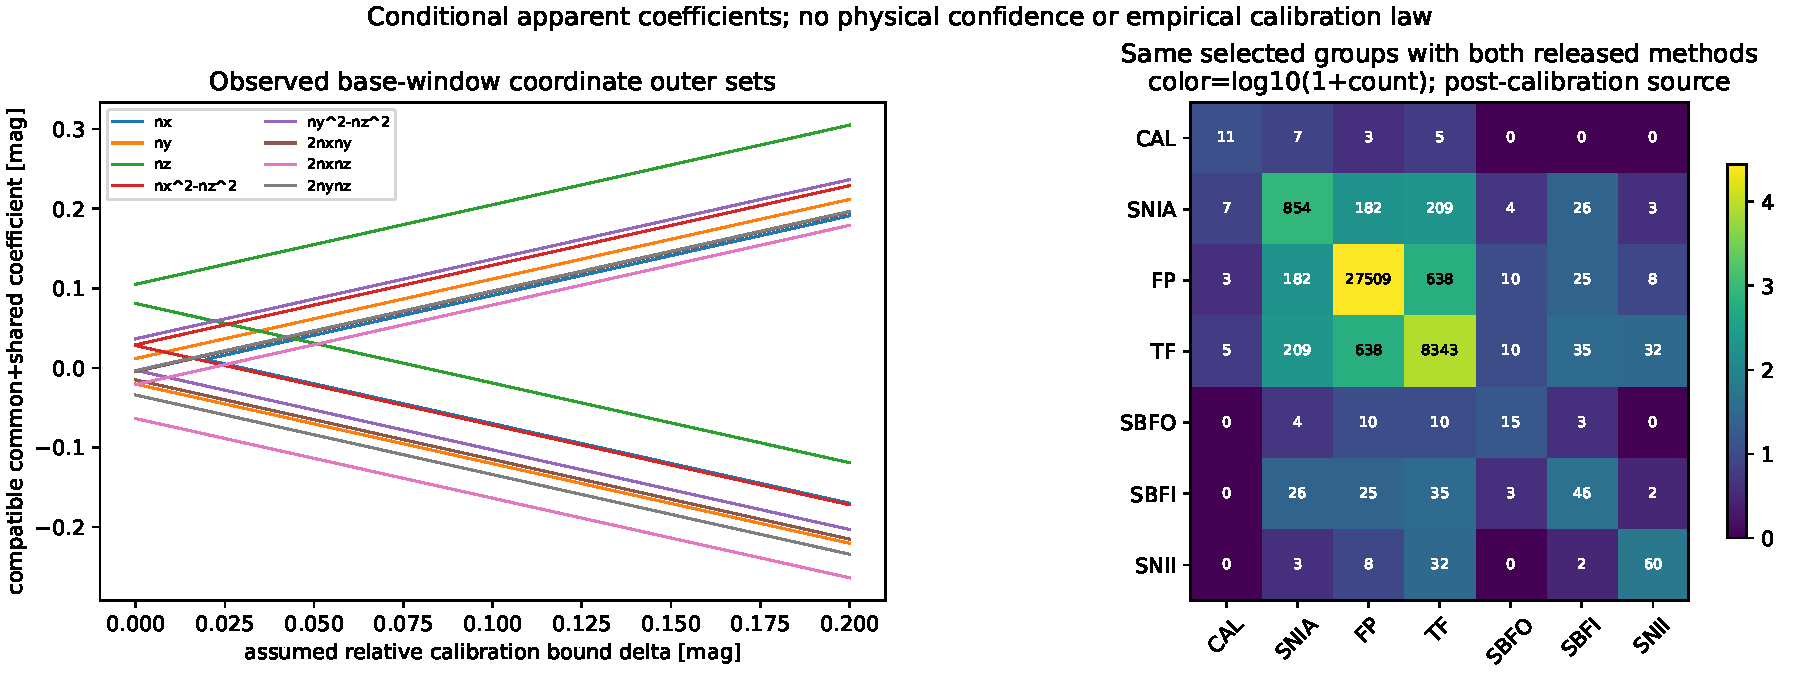
\includegraphics[width=\linewidth,height=.71\textheight,keepaspectratio]{figures/f023_external.pdf}
\caption{Apparent-coordinate outer sets as the allowed common-calibration radius increases (left), and overlap of released distance-method memberships (right). Common calibration and shared group membership affect different parts of the identification problem. These outer sets depend on the stated radius and working source summaries; the overlap does not supply independent likelihood factors or the accepted-subsource selection law.}
\label{fig:f023}
\end{figure}
\clearpage
\begin{figure}[p]
\centering
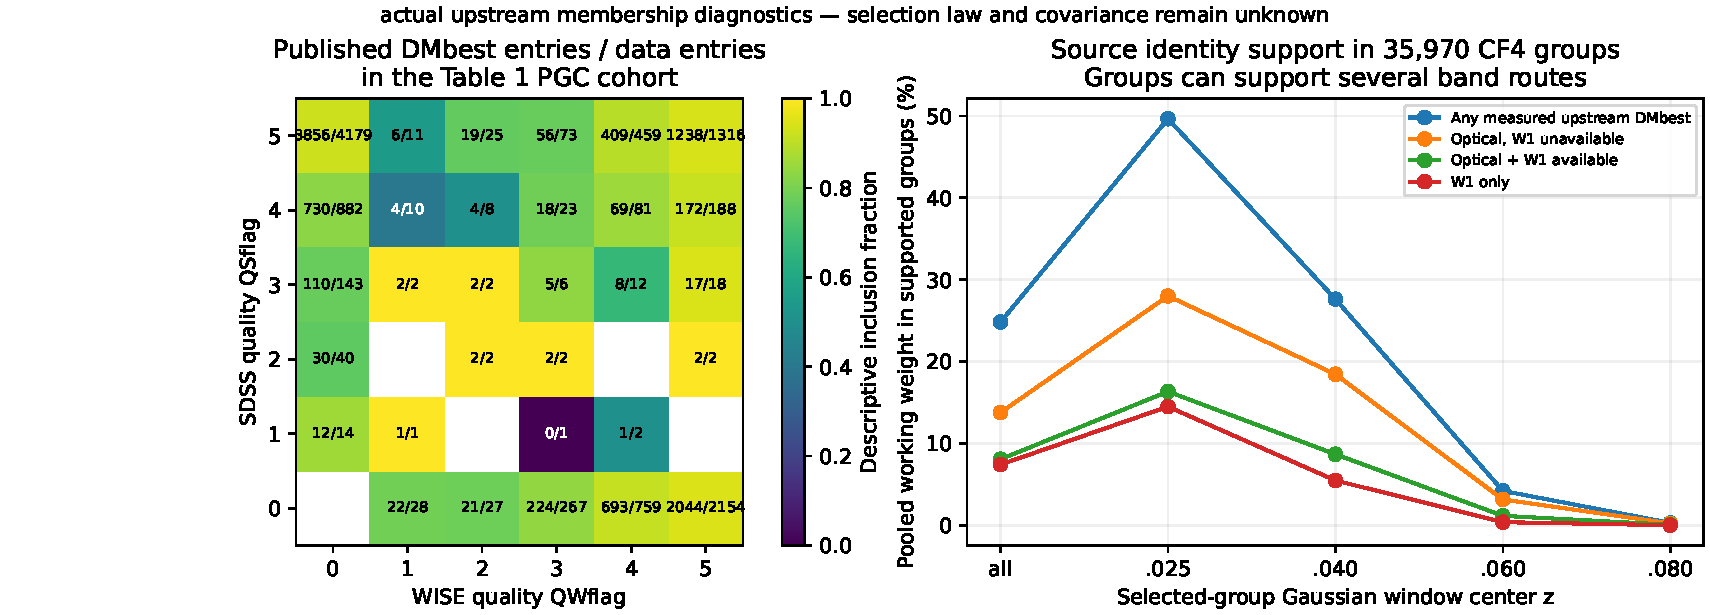
\includegraphics[width=\linewidth,height=.71\textheight,keepaspectratio]{figures/f024_external.pdf}
\caption{Upstream targeting and quality marks in released distance tables. Availability of a best modulus varies with the retained source marks. The table comparisons describe released membership; they do not make quality-dependent missingness ignorable.}
\label{fig:f024}
\end{figure}
\clearpage
\begin{figure}[p]
\centering
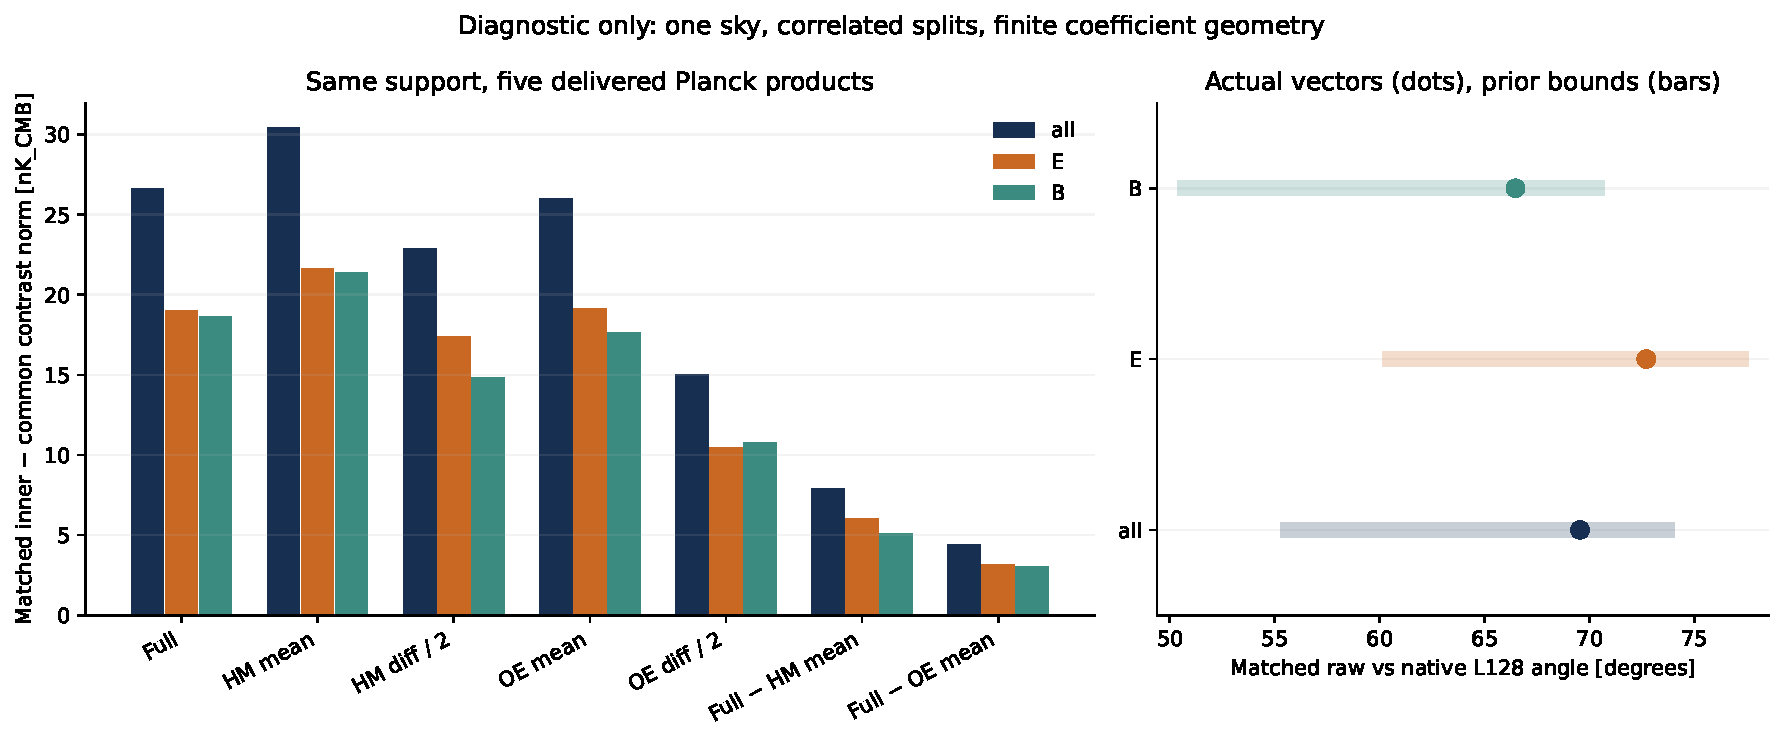
\includegraphics[width=\linewidth,height=.71\textheight,keepaspectratio]{figures/f025.pdf}
\caption{Matched processing contrasts on the same selected sky for five delivered Planck products. Actual vector differences are compared with the corresponding finite geometric bounds. Component norms cannot be added as though the components were aligned, and splits remain correlated views of one sky.}
\label{fig:f025}
\end{figure}
\clearpage
\begin{figure}[p]
\centering
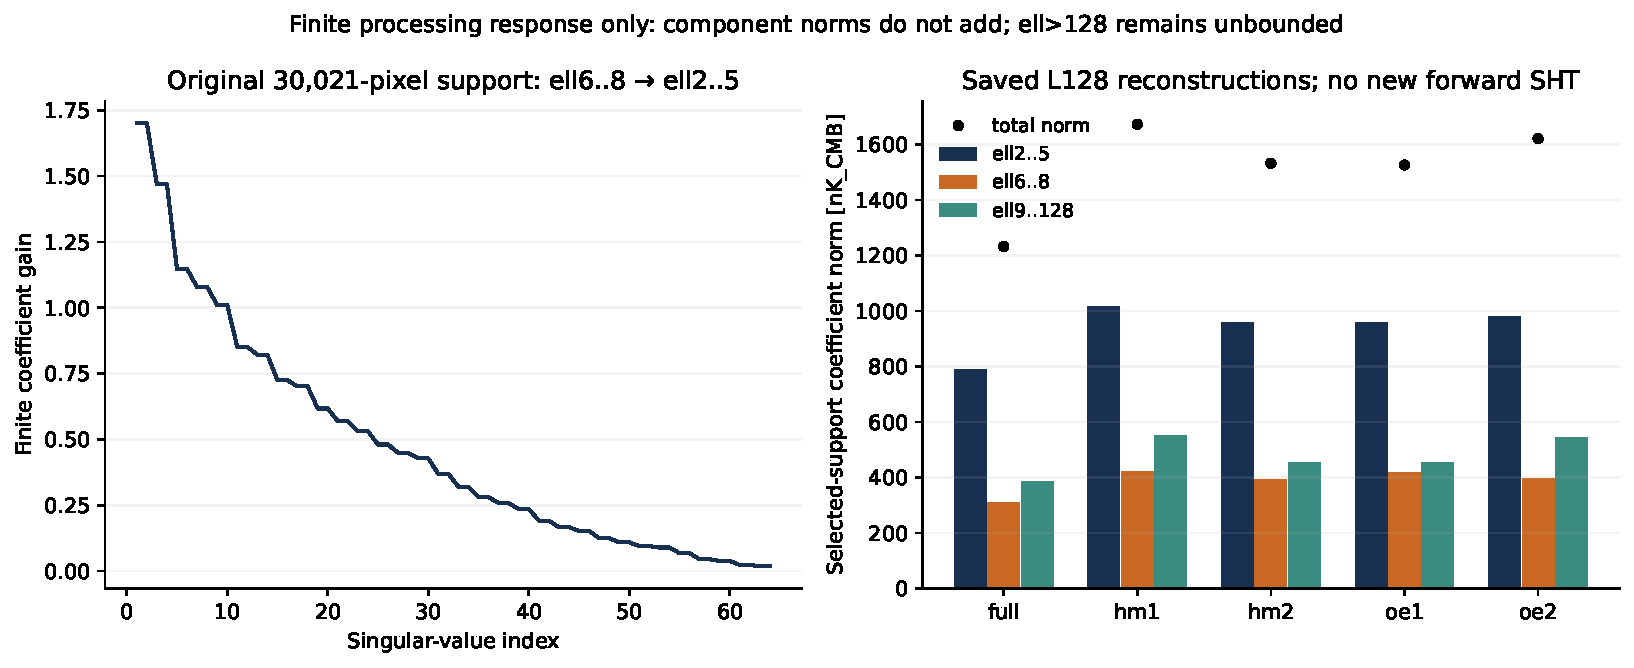
\includegraphics[width=\linewidth,height=.71\textheight,keepaspectratio]{figures/f026.pdf}
\caption{Finite higher-to-lower multipole response on the original selected polarization support. The leakage gains and retained reconstructions quantify an observation operator. Unknown higher-mode amplitudes and the omitted tail are not set to zero; no cosmic B-mode bound follows from operator gain alone.}
\label{fig:f026}
\end{figure}
\clearpage
\begin{figure}[p]
\centering
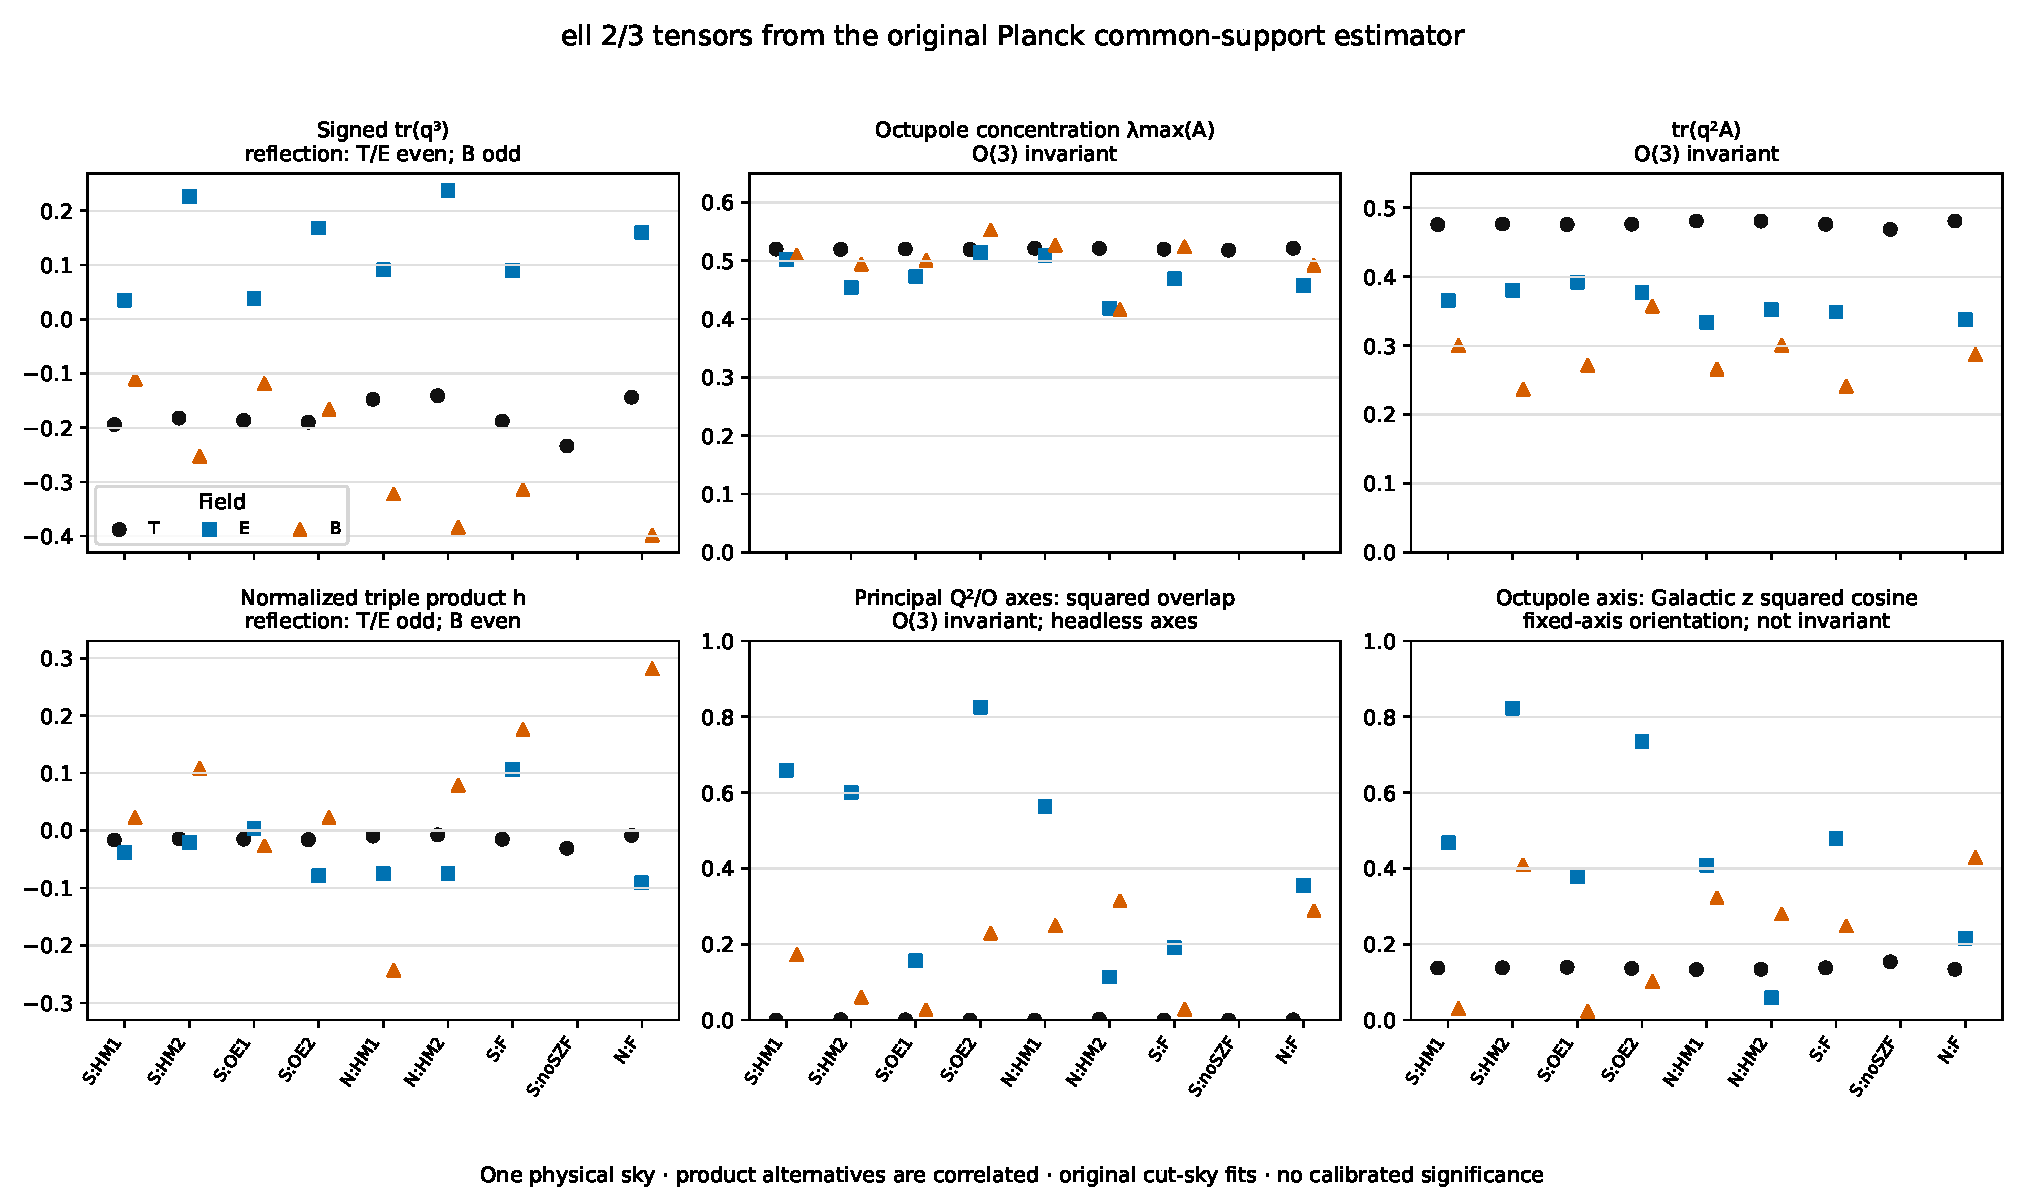
\includegraphics[width=\linewidth,height=.71\textheight,keepaspectratio]{figures/f027_external.pdf}
\caption{Signed shape and orientation descriptors of temperature and polarization multipoles from the original common-support estimator. Polar and axial parity are distinguished. These incomplete descriptors and same-sky product ranges do not provide a calibrated null probability or complete orbit classification.}
\label{fig:f027}
\end{figure}
\clearpage
\begin{figure}[p]
\centering
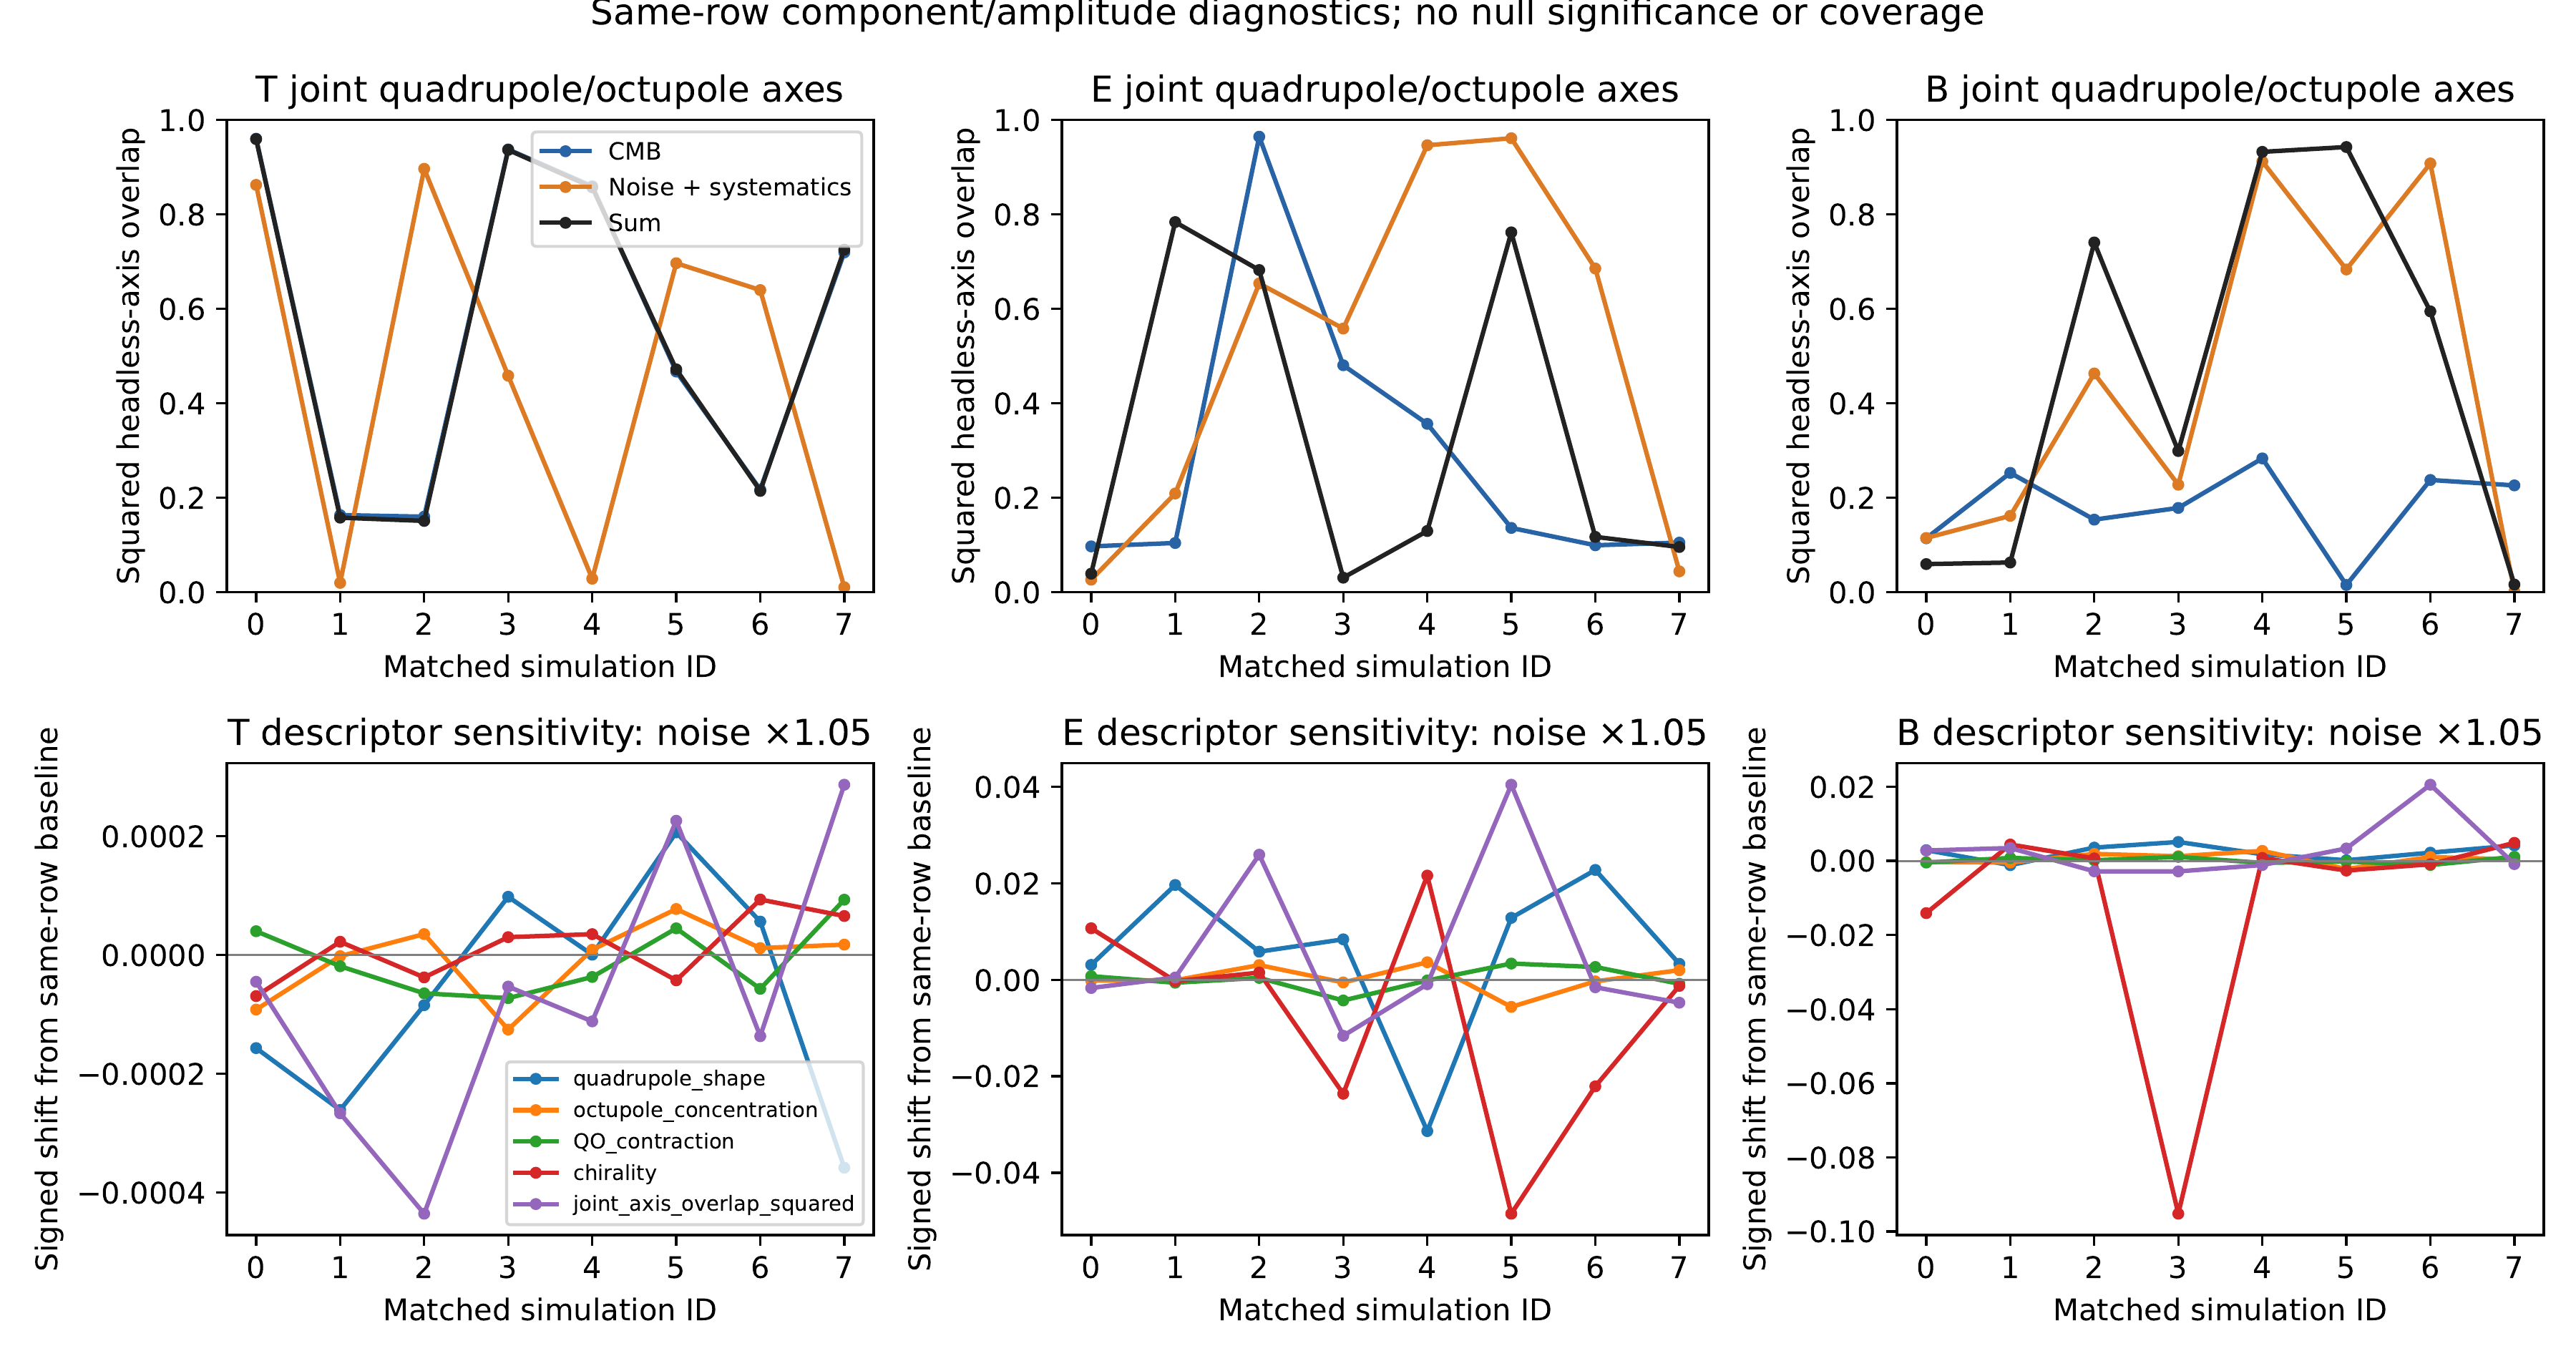
\includegraphics[width=\linewidth,height=.71\textheight,keepaspectratio]{figures/f028_external.png}
\caption{Tensor-descriptor sensitivity in eight matched signal/noise pairs. Each row retains its common source realization and processing. The small pilot and its noise-amplitude perturbation are finite response diagnostics, not an independently calibrated cosmological ensemble.}
\label{fig:f028}
\end{figure}
\clearpage
\begin{figure}[p]
\centering
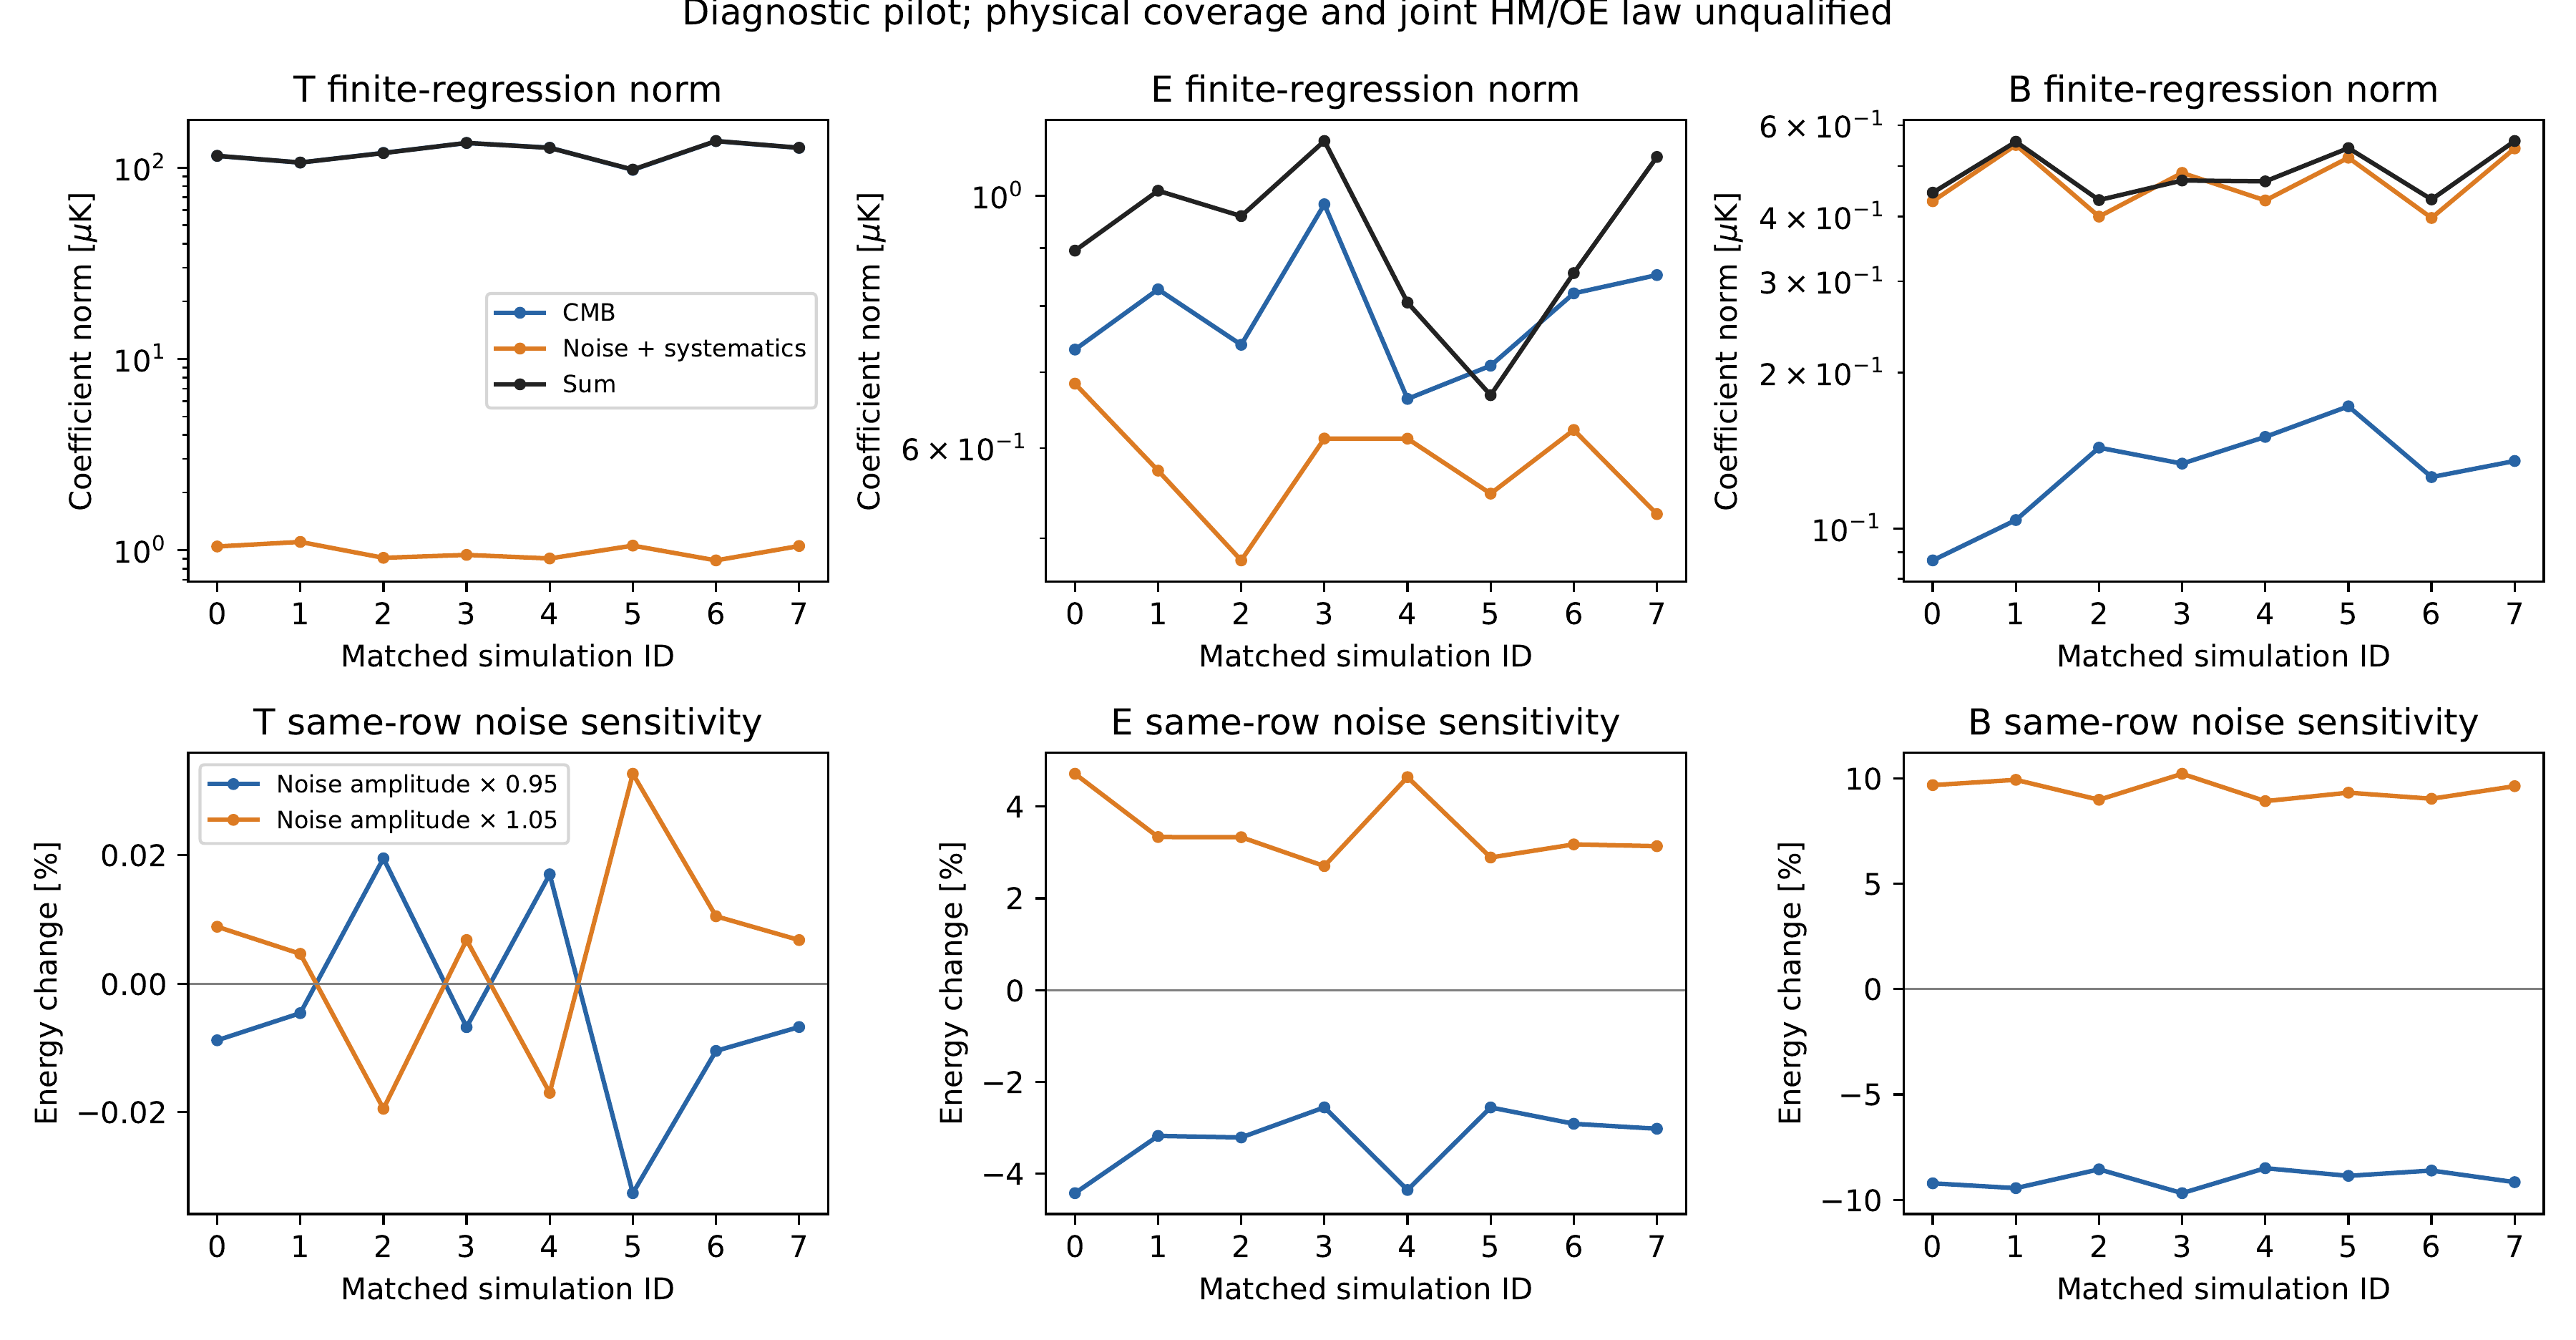
\includegraphics[width=\linewidth,height=.71\textheight,keepaspectratio]{figures/f029_external.png}
\caption{Joint coefficient diagnostics for eight retained Planck signal/noise pairs processed with the same original child-average operator. The centred covariance in the larger joint coordinate space is singular and is not inverted. Physical coverage and the joint half-mission/odd-even source law remain unqualified.}
\label{fig:f029}
\end{figure}
\clearpage
\begin{figure}[p]
\centering
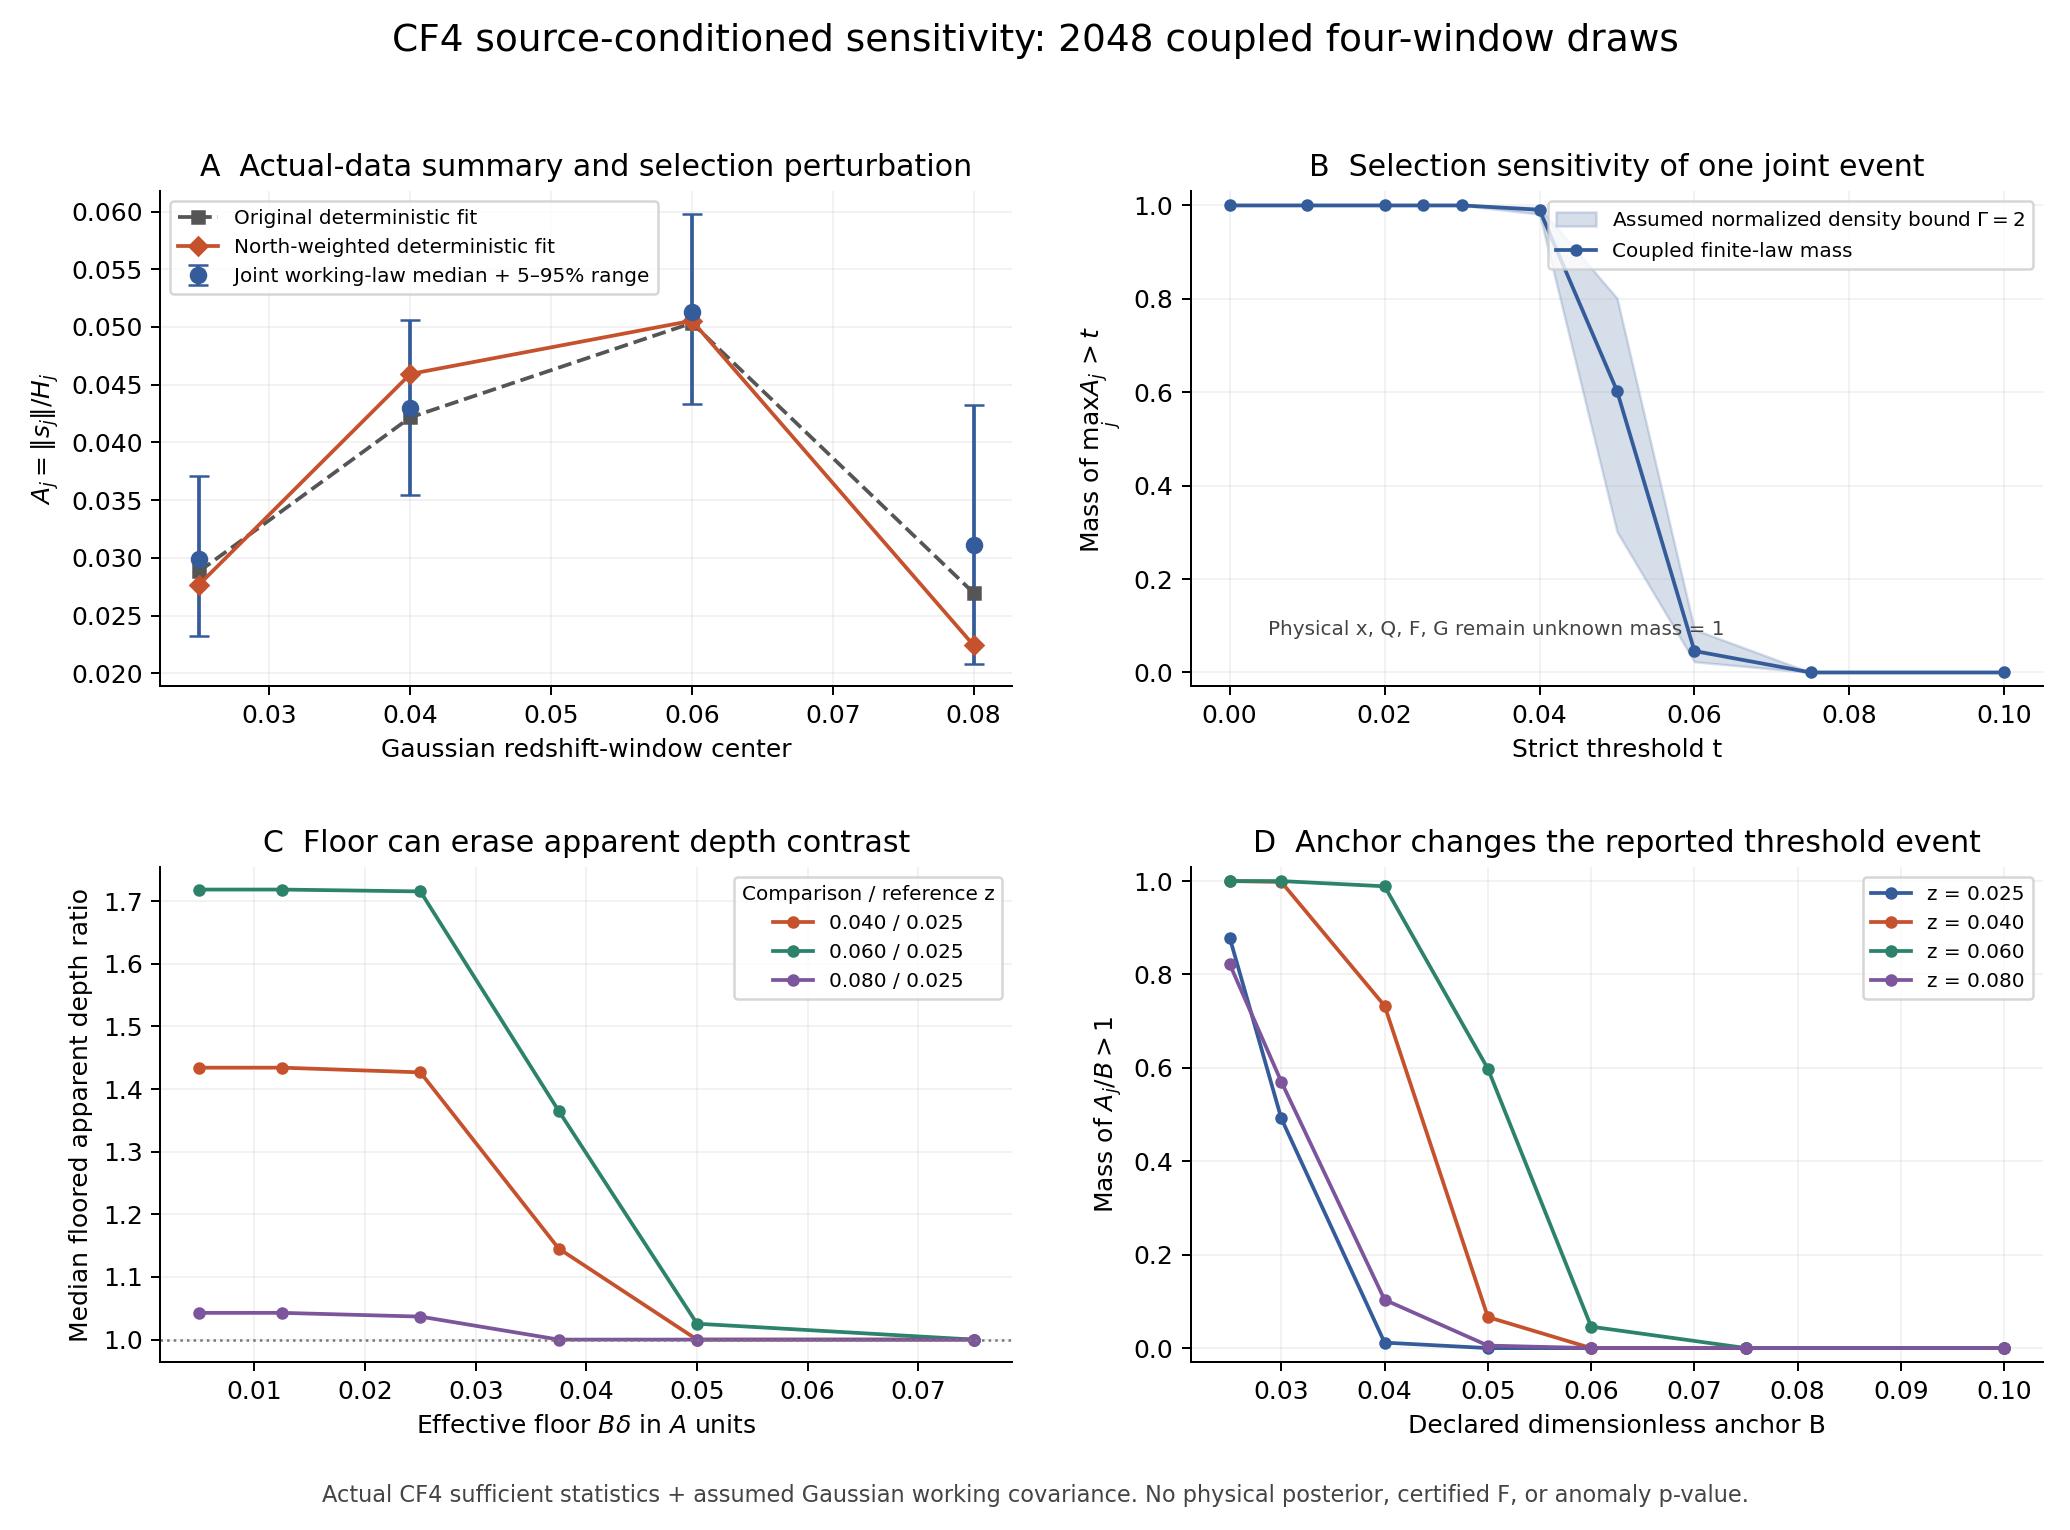
\includegraphics[width=\linewidth,height=.71\textheight,keepaspectratio]{figures/f030.png}
\caption{Functional sensitivity under one coupled finite measure from the four-window Cosmicflows fit. The plots retain common draw identity, declared anchors, positive floors, and strict ties. These are conditional changes in functionals and occupancies, not physical posterior probabilities.}
\label{fig:f030}
\end{figure}
\clearpage
\begin{figure}[p]
\centering
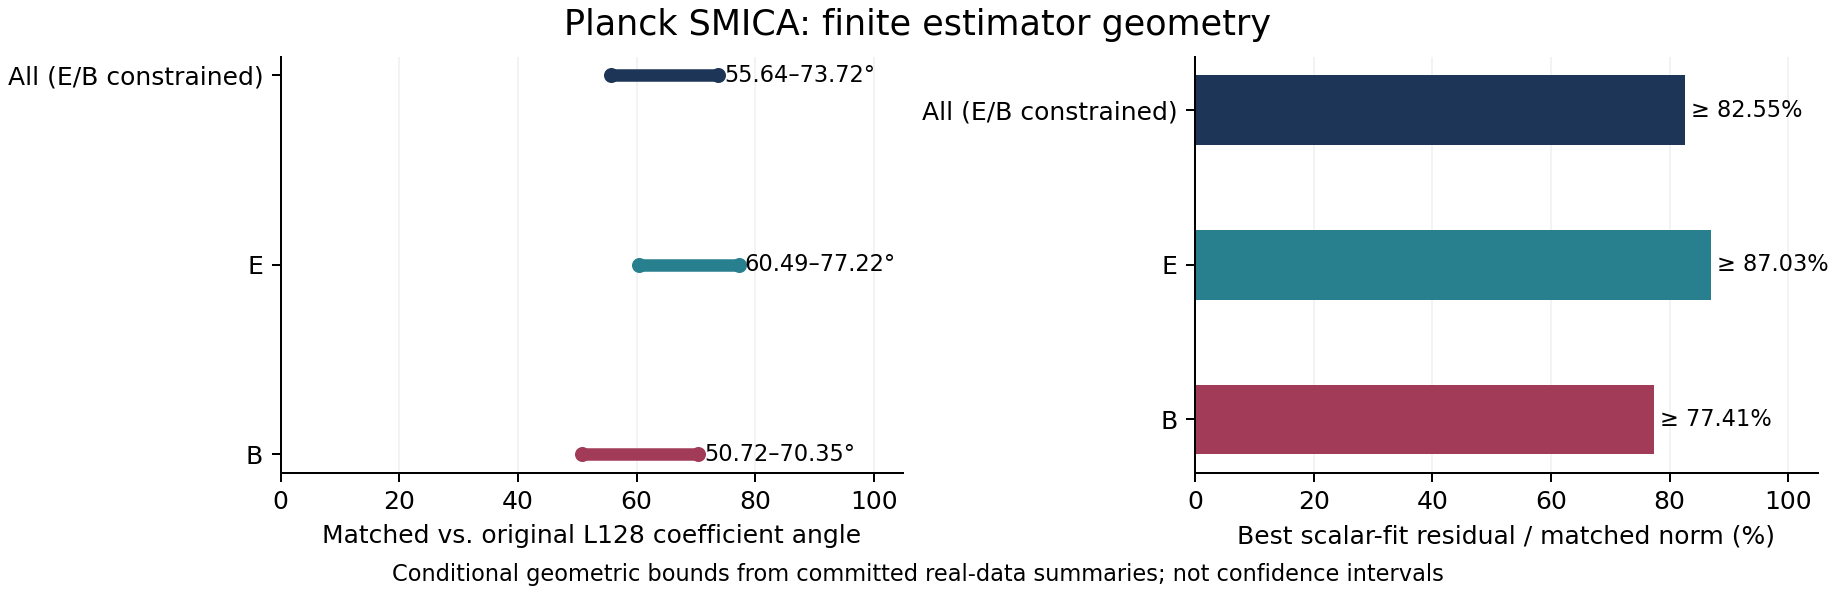
\includegraphics[width=\linewidth,height=.71\textheight,keepaspectratio]{figures/f031.png}
\caption{Finite Planck anchor geometry from the retained processed components. Orthogonal E/B blocks sharpen particular norm bounds, while missing cross orientation limits others. The anchors are computational summaries and do not certify a physical anisotropy ceiling.}
\label{fig:f031}
\end{figure}
\clearpage
\begin{figure}[p]
\centering
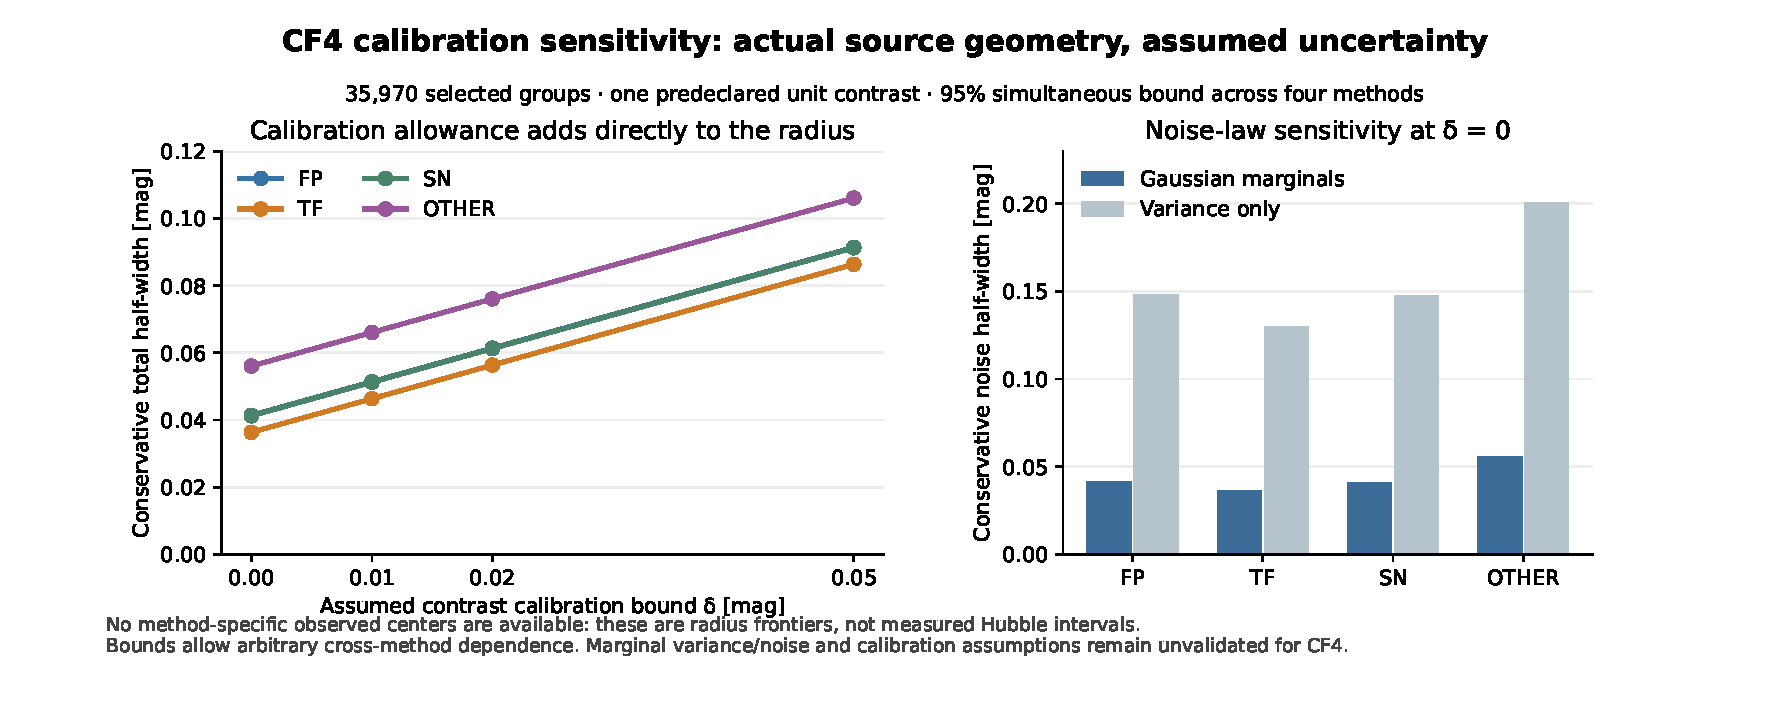
\includegraphics[width=\linewidth,height=.71\textheight,keepaspectratio]{figures/f032_external.pdf}
\caption{Calibration-radius sensitivity on the actual Cosmicflows source geometry. The selected contrast and simultaneous working reference are fixed; the horizontal radius is assumed. A radius-only frontier does not supply observed calibration centres or an empirically measured systematic bound.}
\label{fig:f032}
\end{figure}
\clearpage
\begin{figure}[p]
\centering
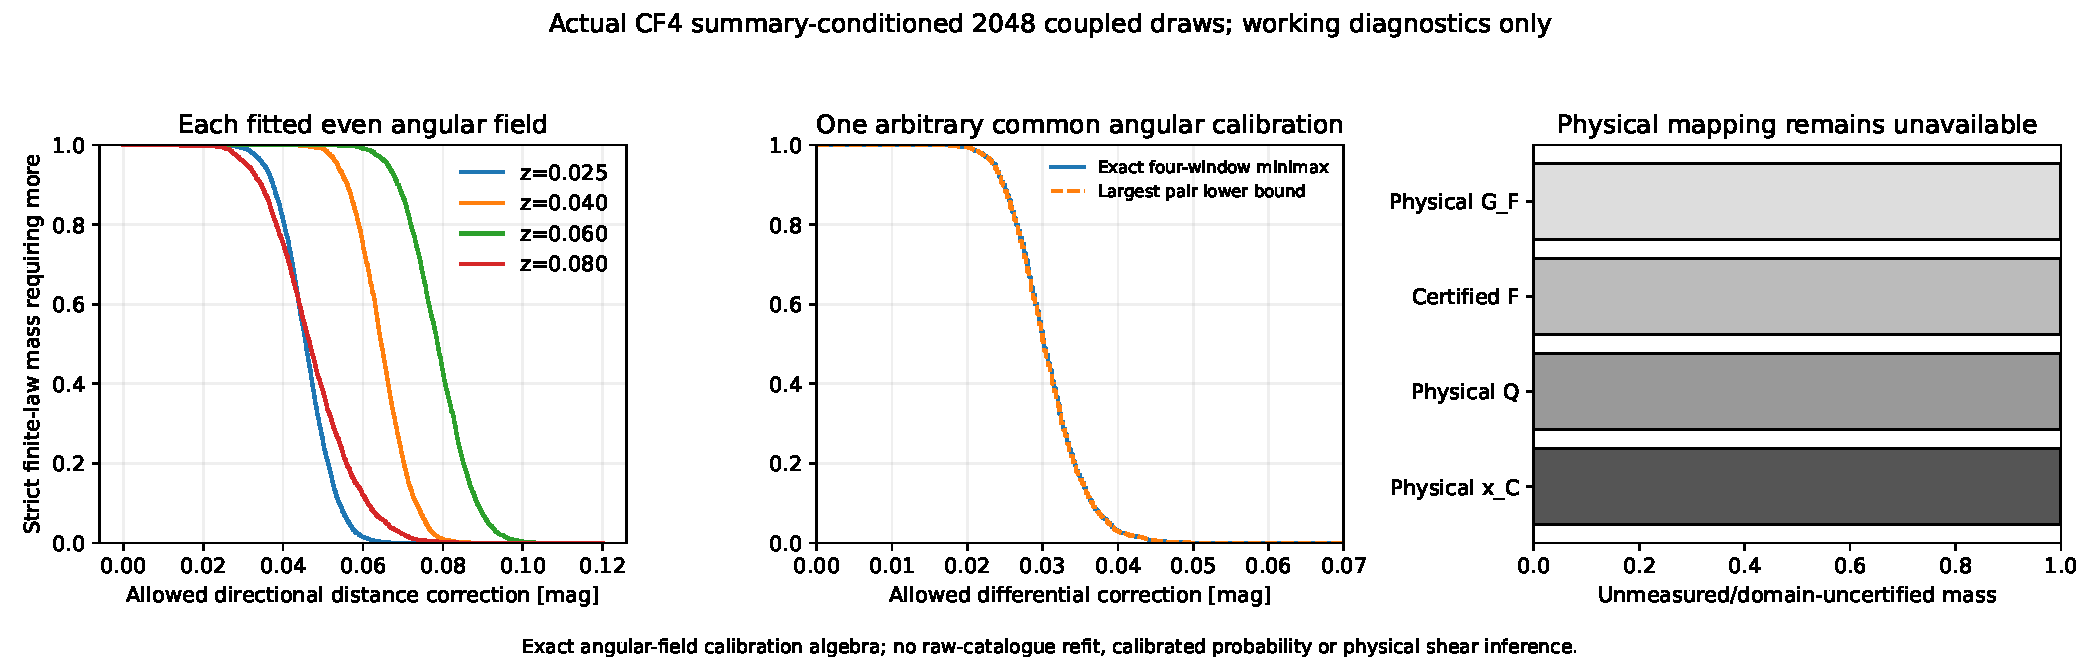
\includegraphics[width=\linewidth,height=.71\textheight,keepaspectratio]{figures/f033_external.pdf}
\caption{Calibration obstruction for the coupled group-fit finite measure. The panels distinguish independently fitted angular fields from one shared angular calibration. Their exceedances refer to the retained working measure, with physical completion and source covariance still unqualified.}
\label{fig:f033}
\end{figure}
\clearpage
\begin{figure}[p]
\centering
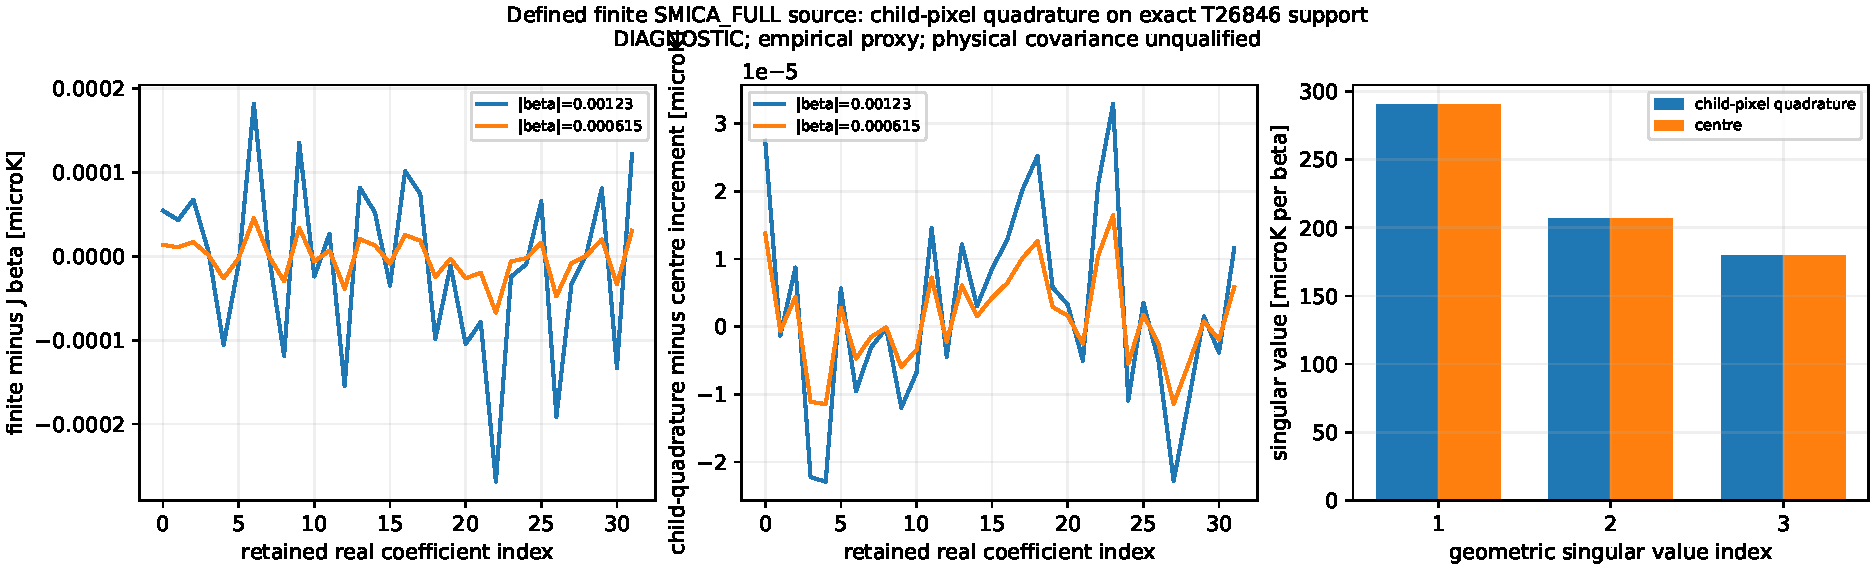
\includegraphics[width=\linewidth,height=.71\textheight,keepaspectratio]{figures/f034_external.pdf}
\caption{Finite delivered-map observer-response calculation at child-pixel resolution, compared with a pixel-centre approximation. The mask and source field are fixed. Differences and finite-minus-linear residuals characterize that processing response, not a cosmological transfer history or calibrated spatial covariance.}
\label{fig:f034}
\end{figure}
\clearpage
\begin{figure}[p]
\centering
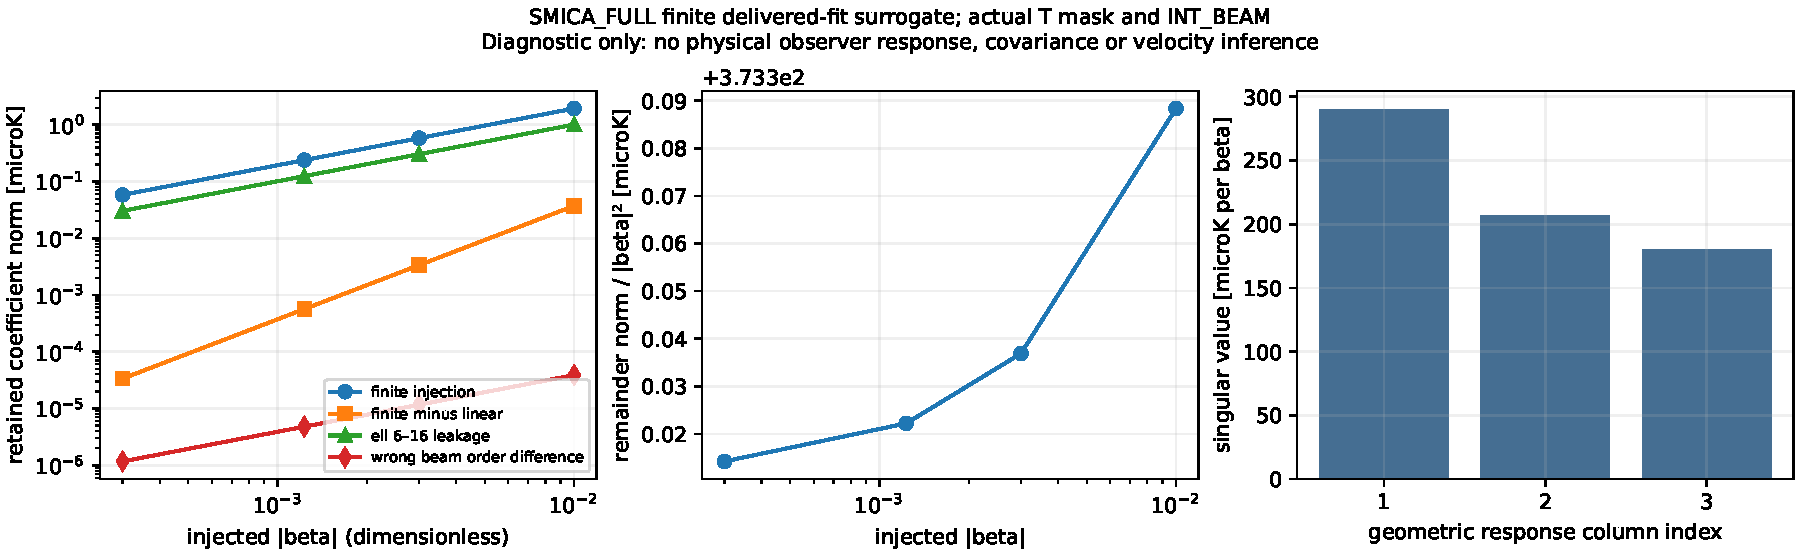
\includegraphics[width=\linewidth,height=.71\textheight,keepaspectratio]{figures/f035.pdf}
\caption{Finite observer-boost interventions and linear-response residuals for a declared delivered map. Higher-mode content and beam order alter the result. The curves test this finite response model; they do not establish a complete physical source history or null law.}
\label{fig:f035}
\end{figure}
\clearpage
\begin{figure}[p]
\centering
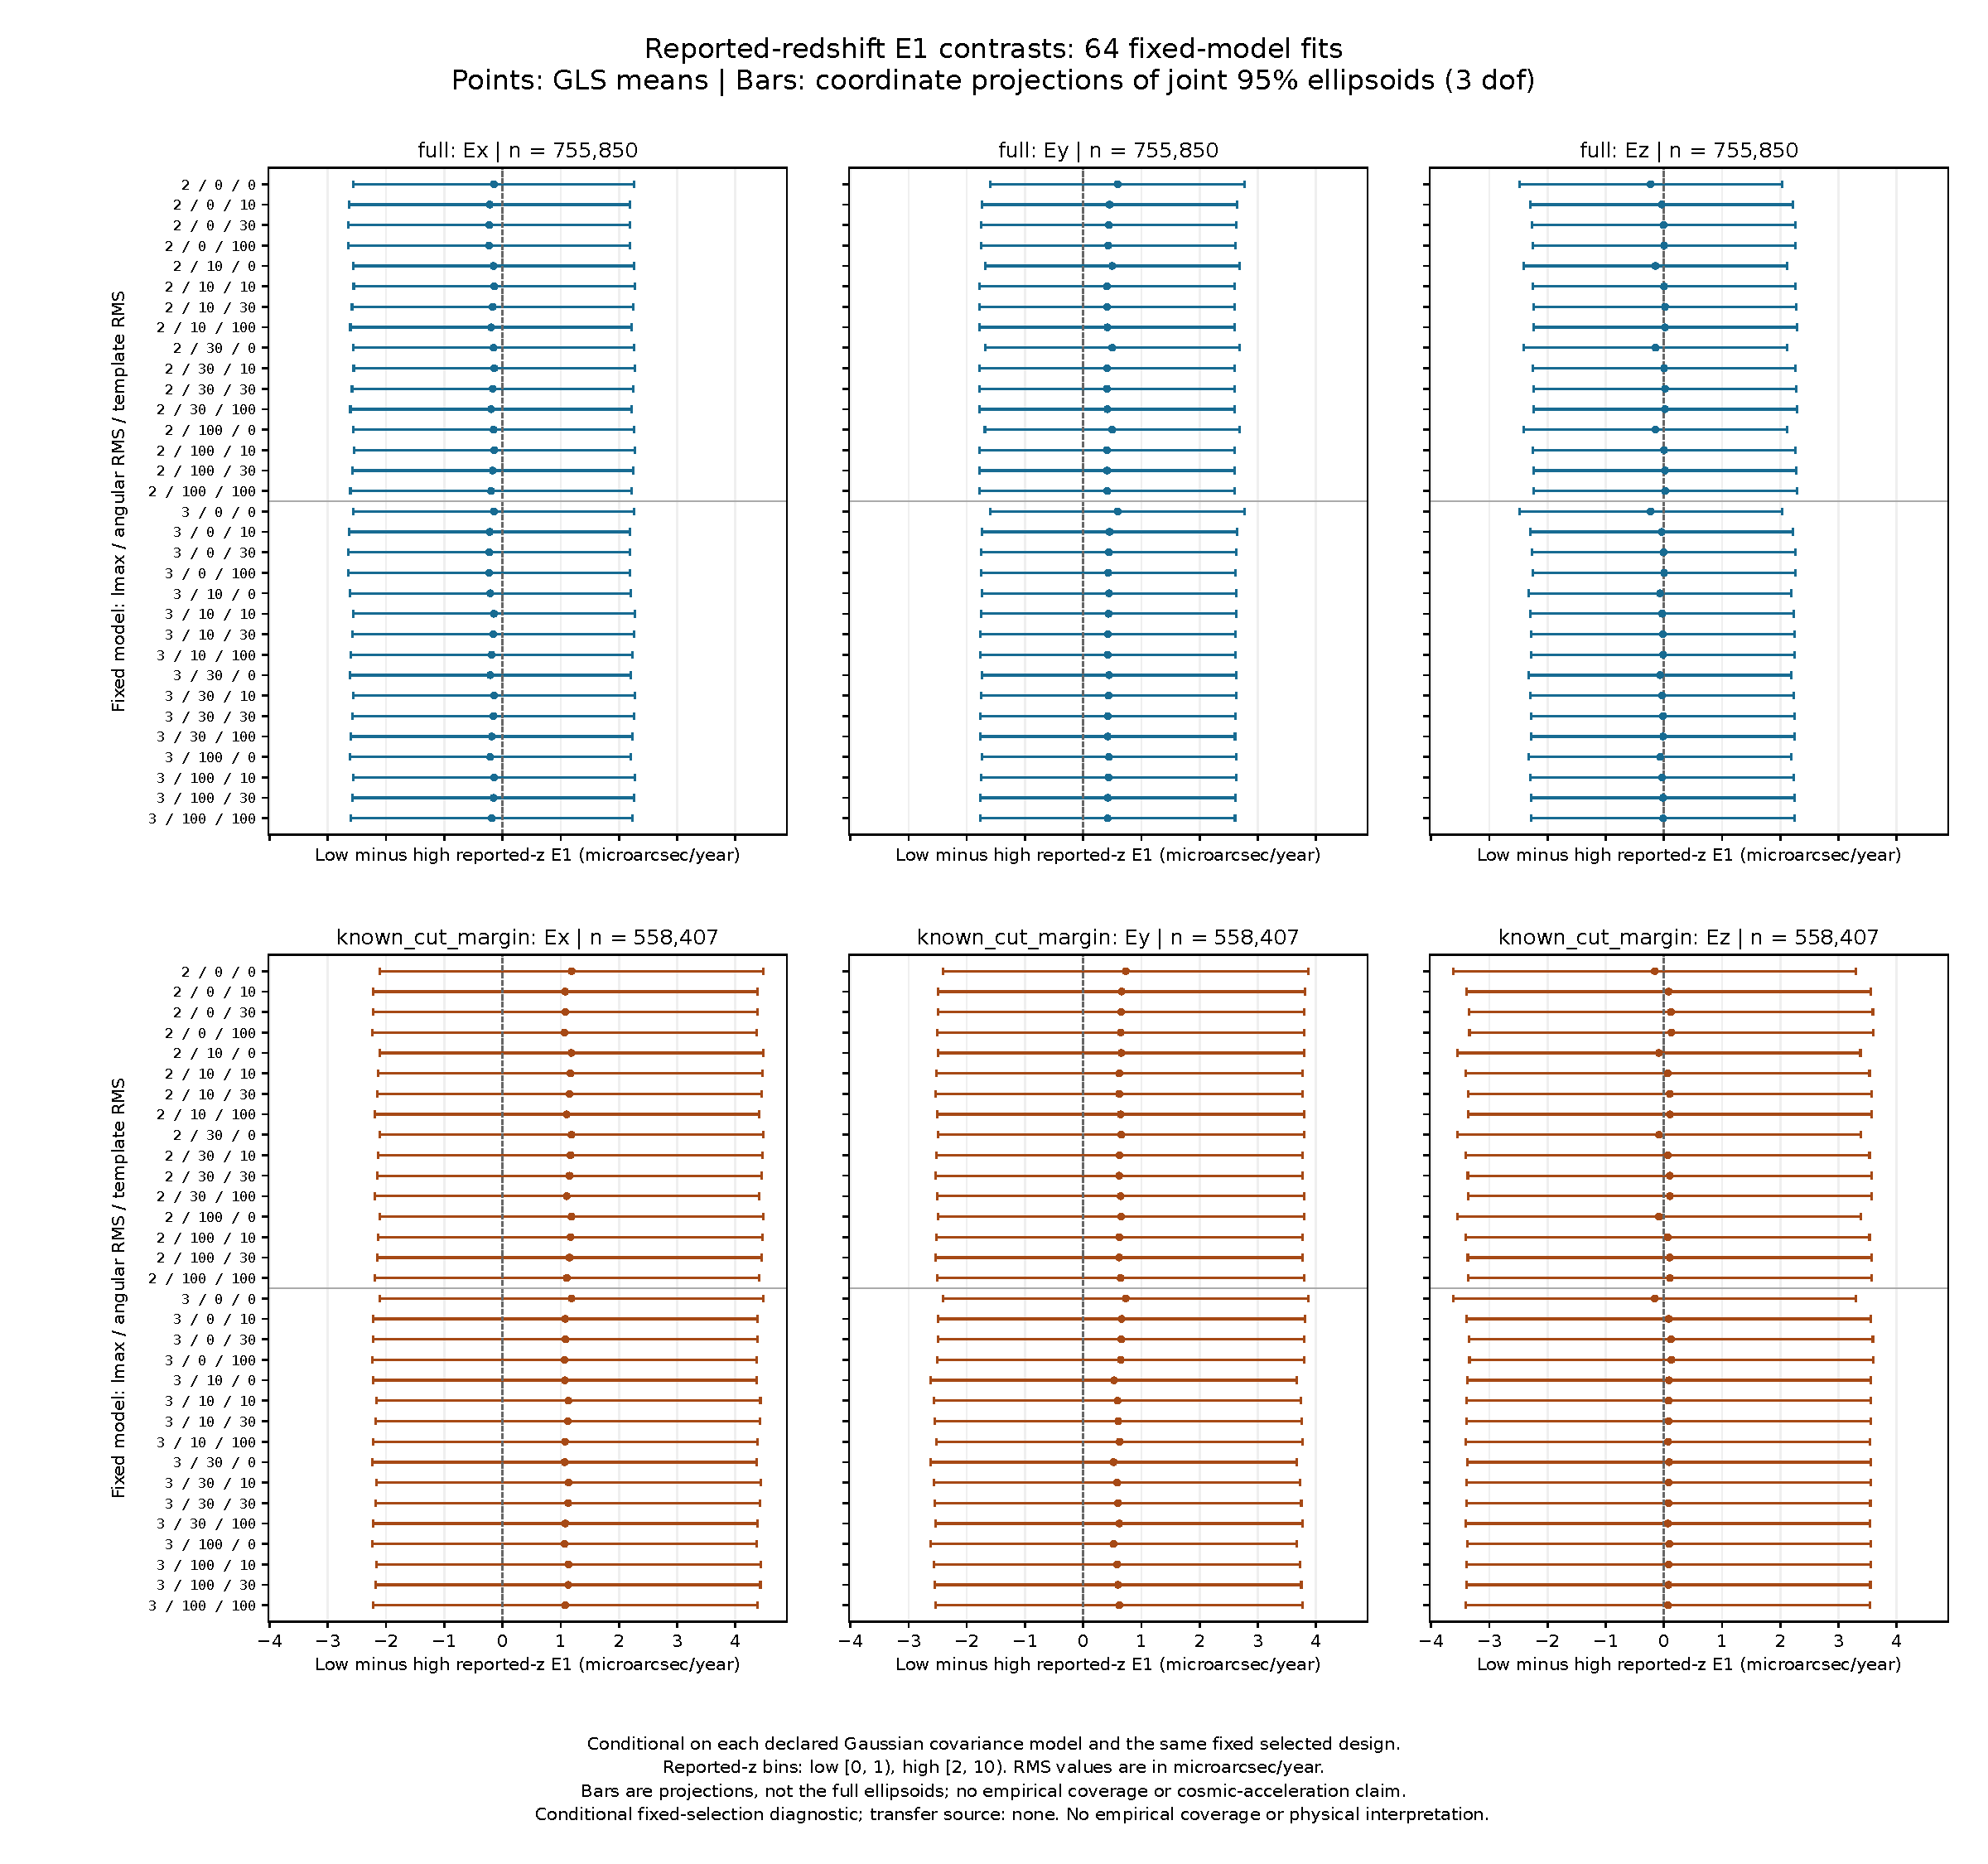
\includegraphics[width=\linewidth,height=.71\textheight,keepaspectratio]{figures/f036_external.pdf}
\caption{Low-minus-high reported-redshift astrometric contrast under the stated covariance scenarios. Shared bins and nuisance responses are retained. This is a conditional coordinate contrast; reported redshift, spatial covariance, and source-centroid response are not a calibrated physical depth experiment.}
\label{fig:f036}
\end{figure}
\clearpage
\begin{figure}[p]
\centering
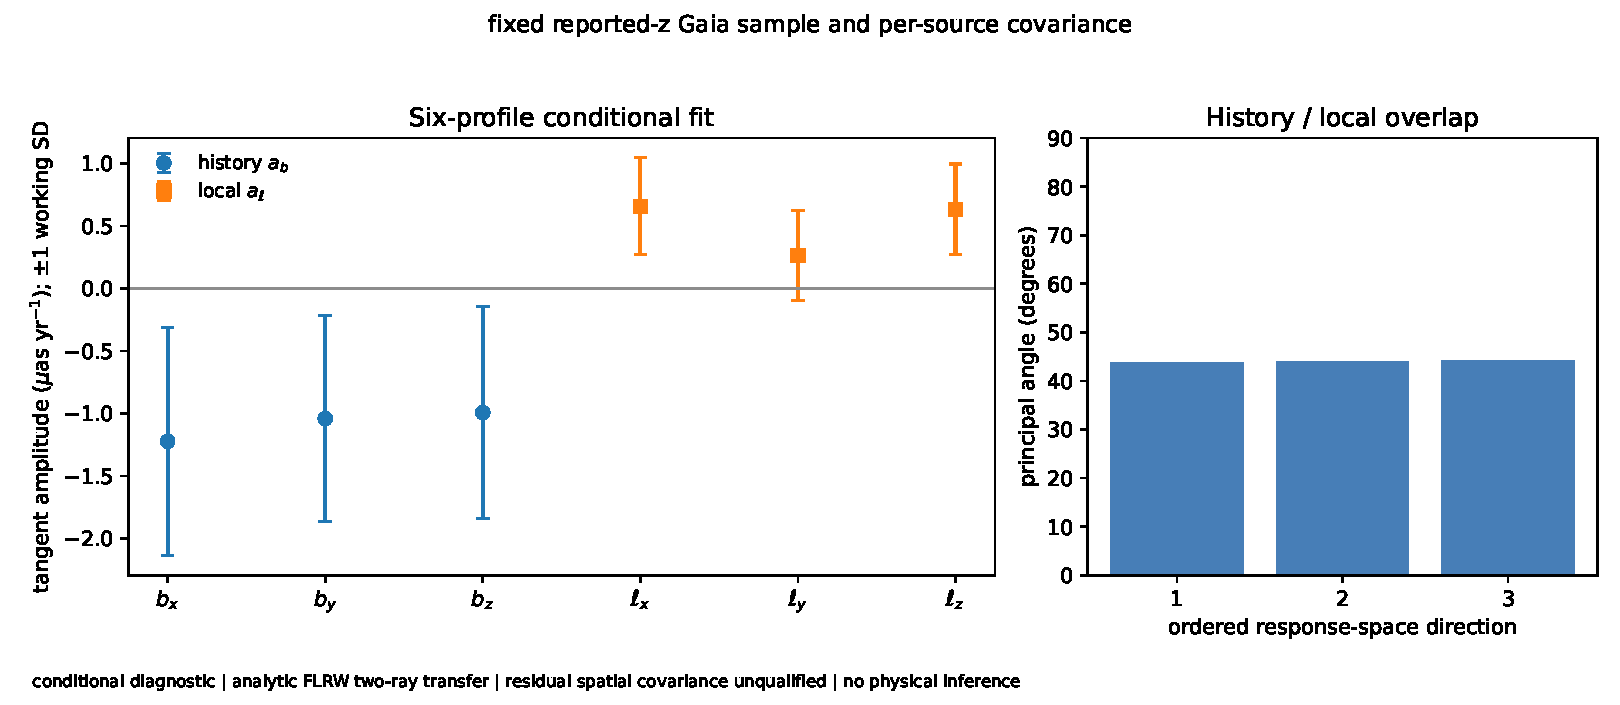
\includegraphics[width=\linewidth,height=.71\textheight,keepaspectratio]{figures/f037_external.pdf}
\caption{Profiled history and local-response coefficients and their principal-angle geometry in the retained astrometric design. Error bars use the stated working covariance. Full rank does not imply useful power within a small-response domain or establish a physical history.}
\label{fig:f037}
\end{figure}
\clearpage
\begin{figure}[p]
\centering
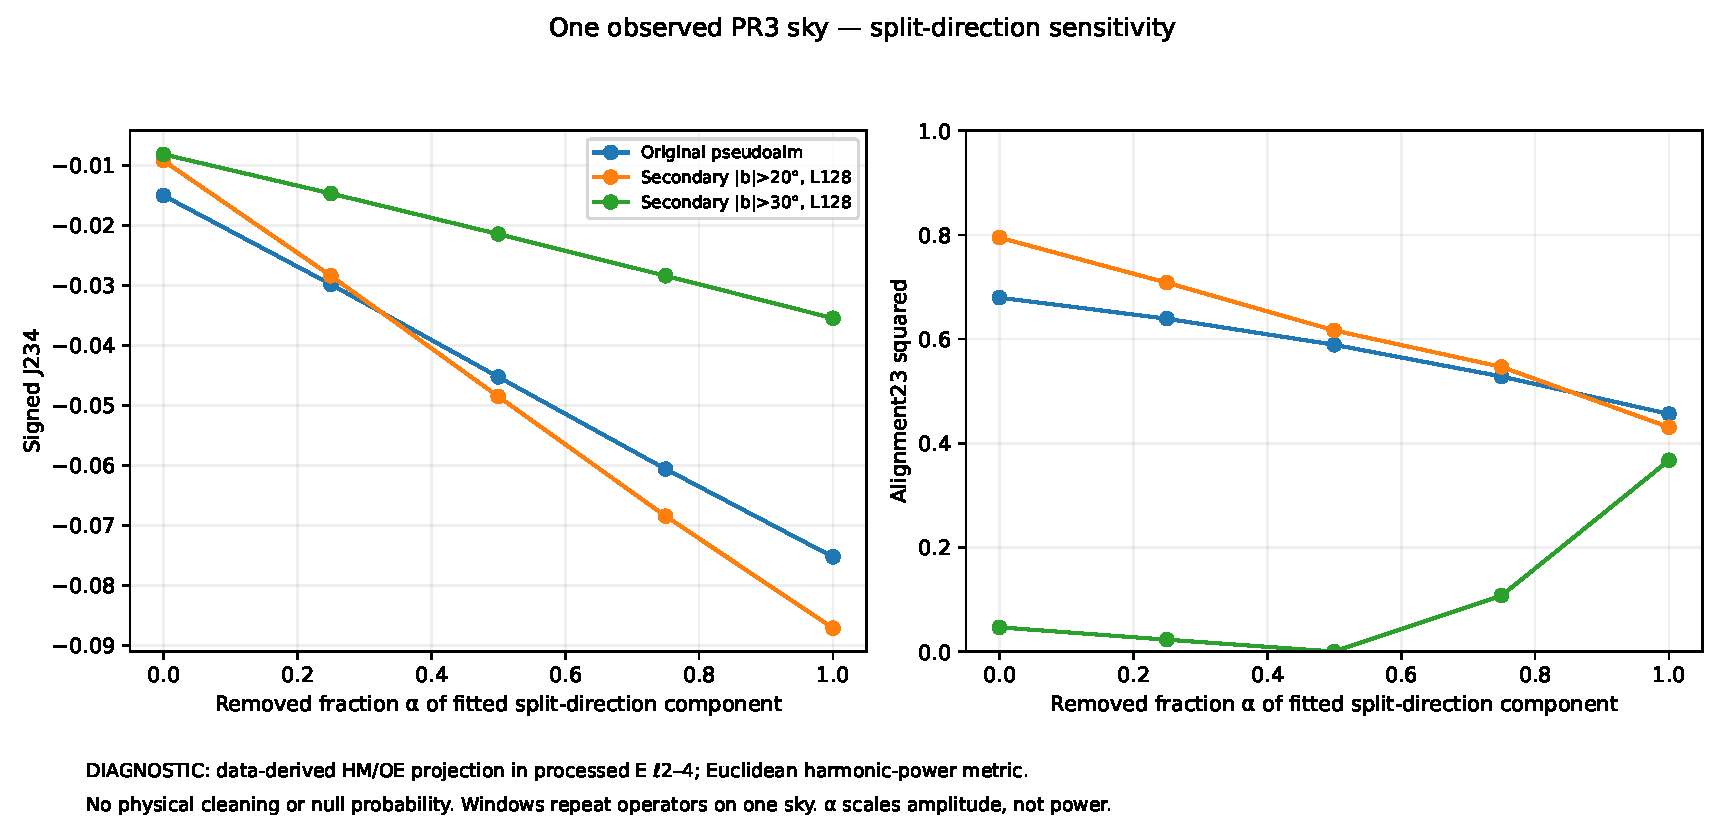
\includegraphics[width=\linewidth,height=.71\textheight,keepaspectratio]{figures/f039_external.pdf}
\caption{Sensitivity of processed E-pseudoalm morphology to split-direction projections on one Planck sky. The processing windows remain distinct. These projected comparisons do not remove an arbitrary common foreground or supply an exchangeable physical null.}
\label{fig:f039}
\end{figure}
\clearpage
\begin{figure}[p]
\centering
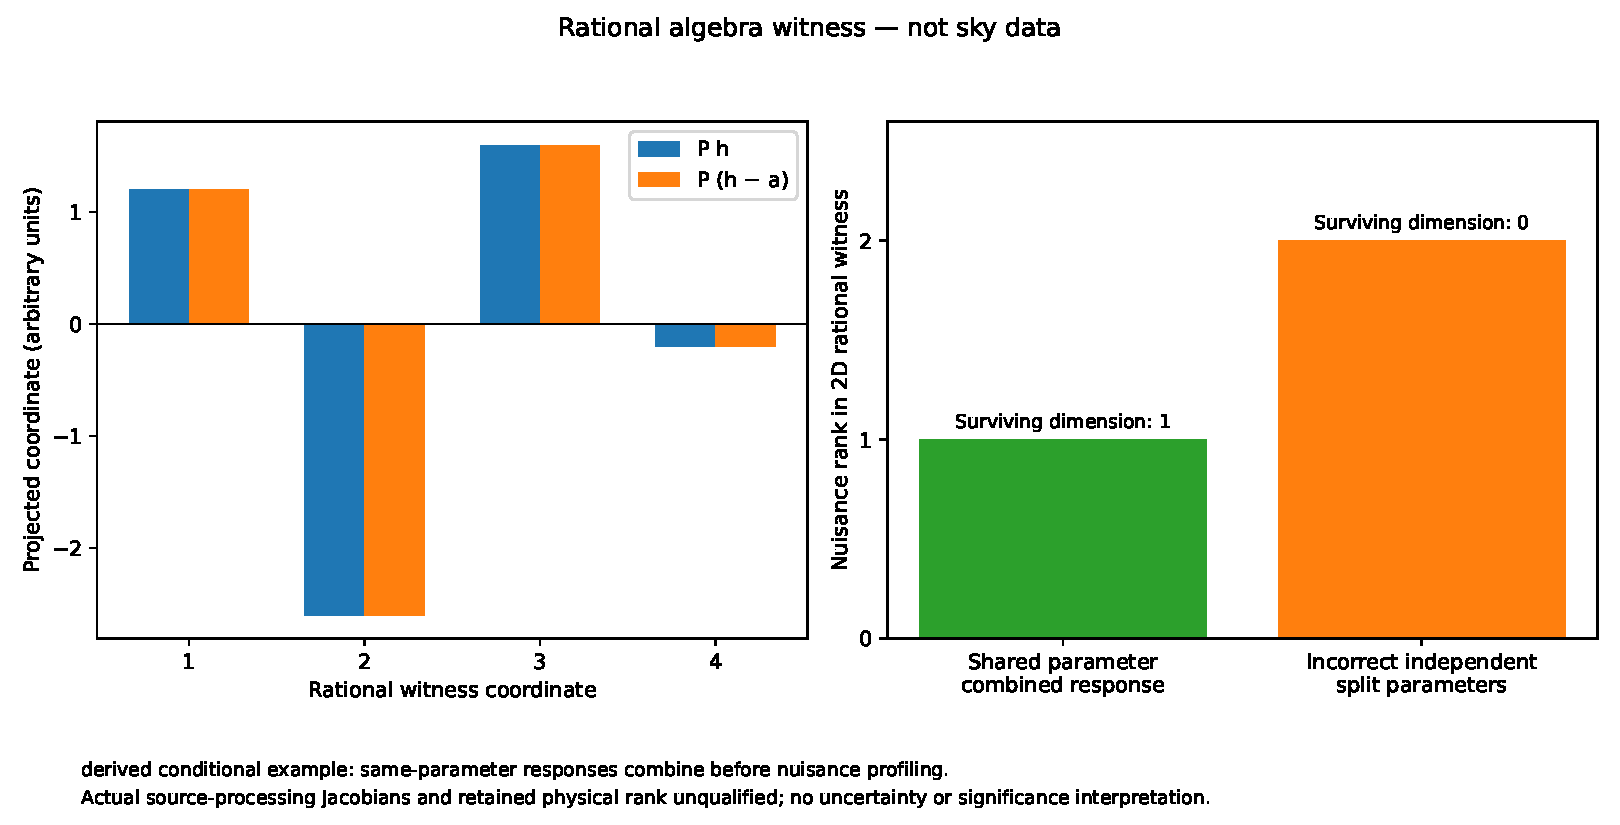
\includegraphics[width=\linewidth,height=.71\textheight,keepaspectratio]{figures/f040_external.pdf}
\caption{Exact rational nuisance-quotient counterexample. The displayed vectors and rank changes are constructed algebraic witnesses, not sky measurements. They show why a response can survive one nuisance span and disappear under a larger one.}
\label{fig:f040}
\end{figure}
\clearpage
\begin{figure}[p]
\centering
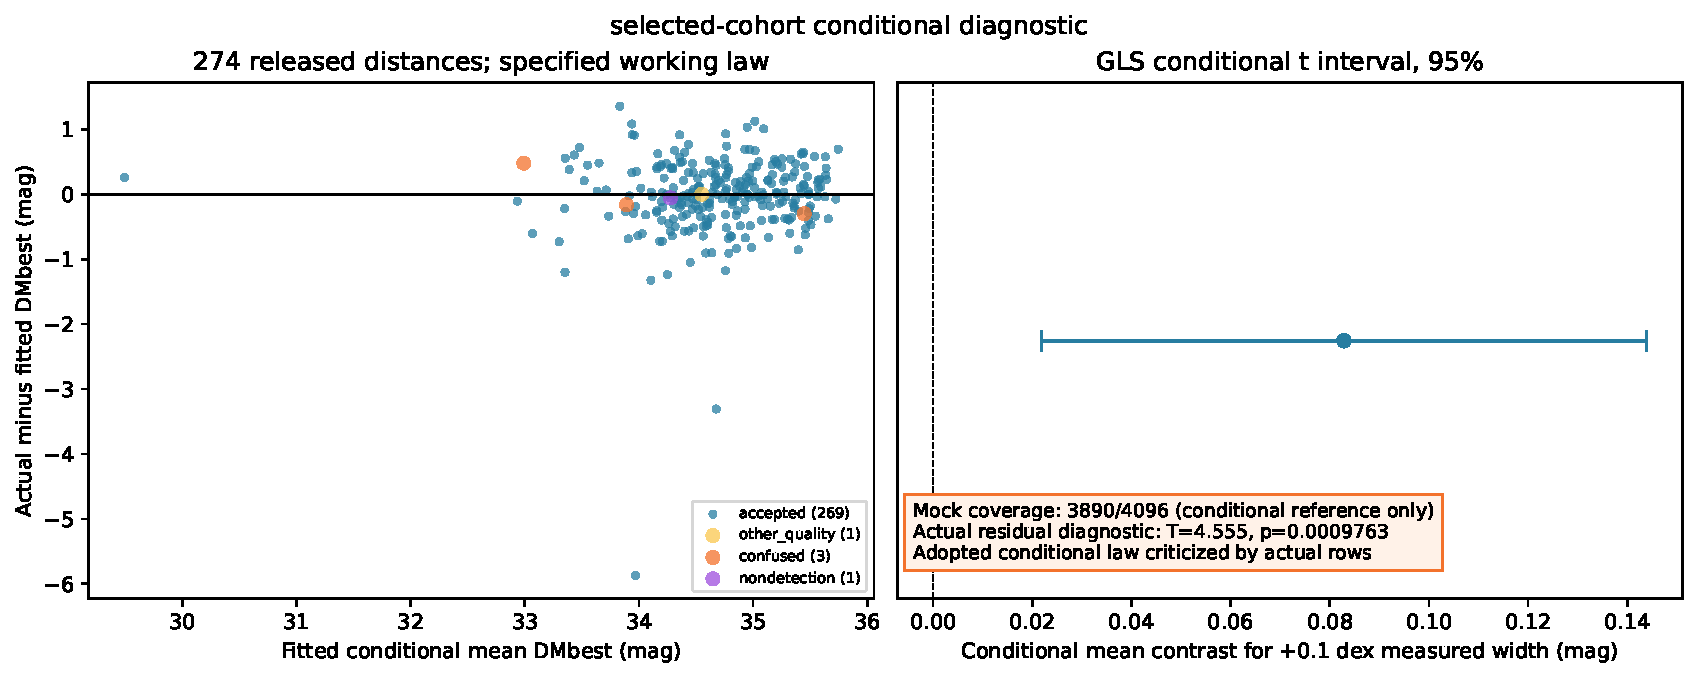
\includegraphics[width=\linewidth,height=.71\textheight,keepaspectratio]{figures/f041_external.pdf}
\caption{Actual-data residual criticism of the earlier selected-distance Gaussian model. The retained quality marks and simulation reference expose its failure on the observed cohort. Simulations generated under that model do not repair the failed actual-data check or validate later model variants.}
\label{fig:f041}
\end{figure}
\clearpage
\begin{figure}[p]
\centering
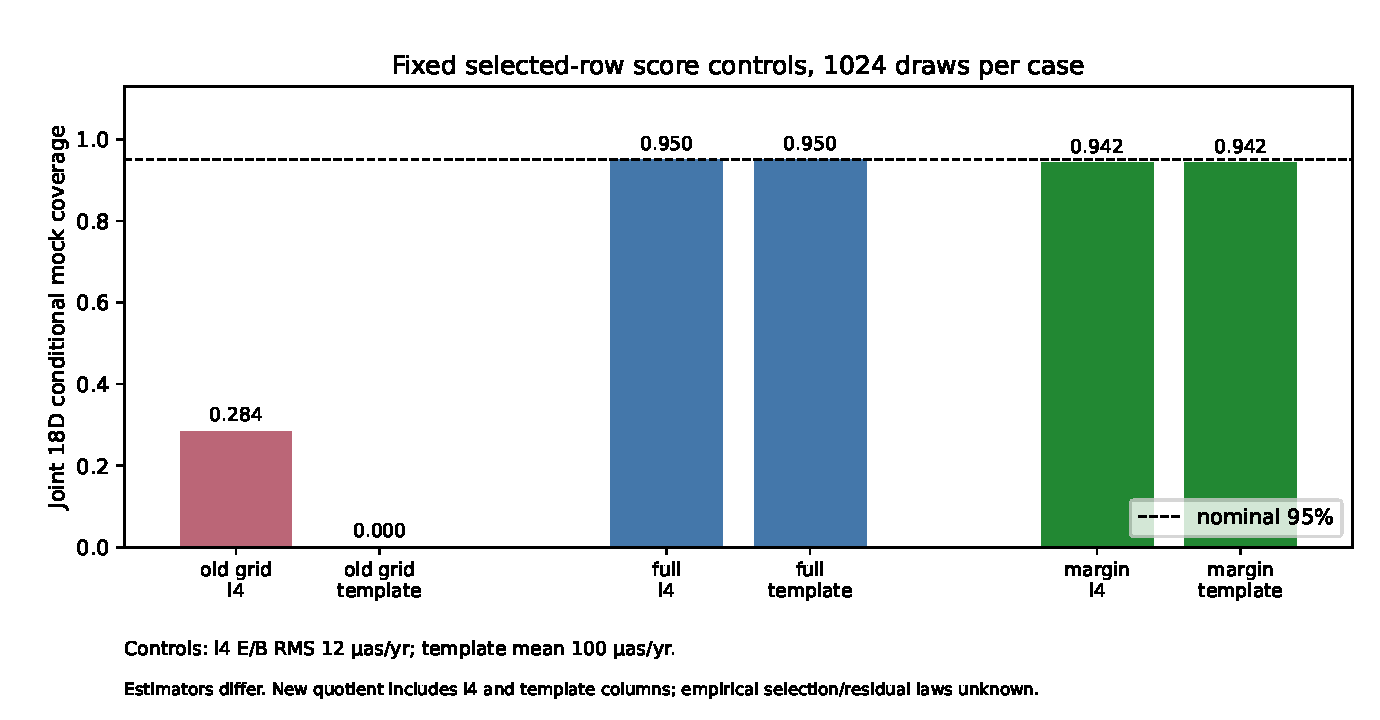
\includegraphics[width=\linewidth,height=.71\textheight,keepaspectratio]{figures/f042_external.pdf}
\caption{Synthetic astrometric coverage controls over 1024 realizations, comparing full and marginal fits under the stated generated laws. Omitted higher-order E4/B4 structure and a template-correlated mean substantially degrade nominal joint coverage. These are misspecification examples; they do not measure physical Gaia coverage or calibrate the actual spatial covariance.}
\label{fig:f042}
\end{figure}
\clearpage
\begin{figure}[p]
\centering
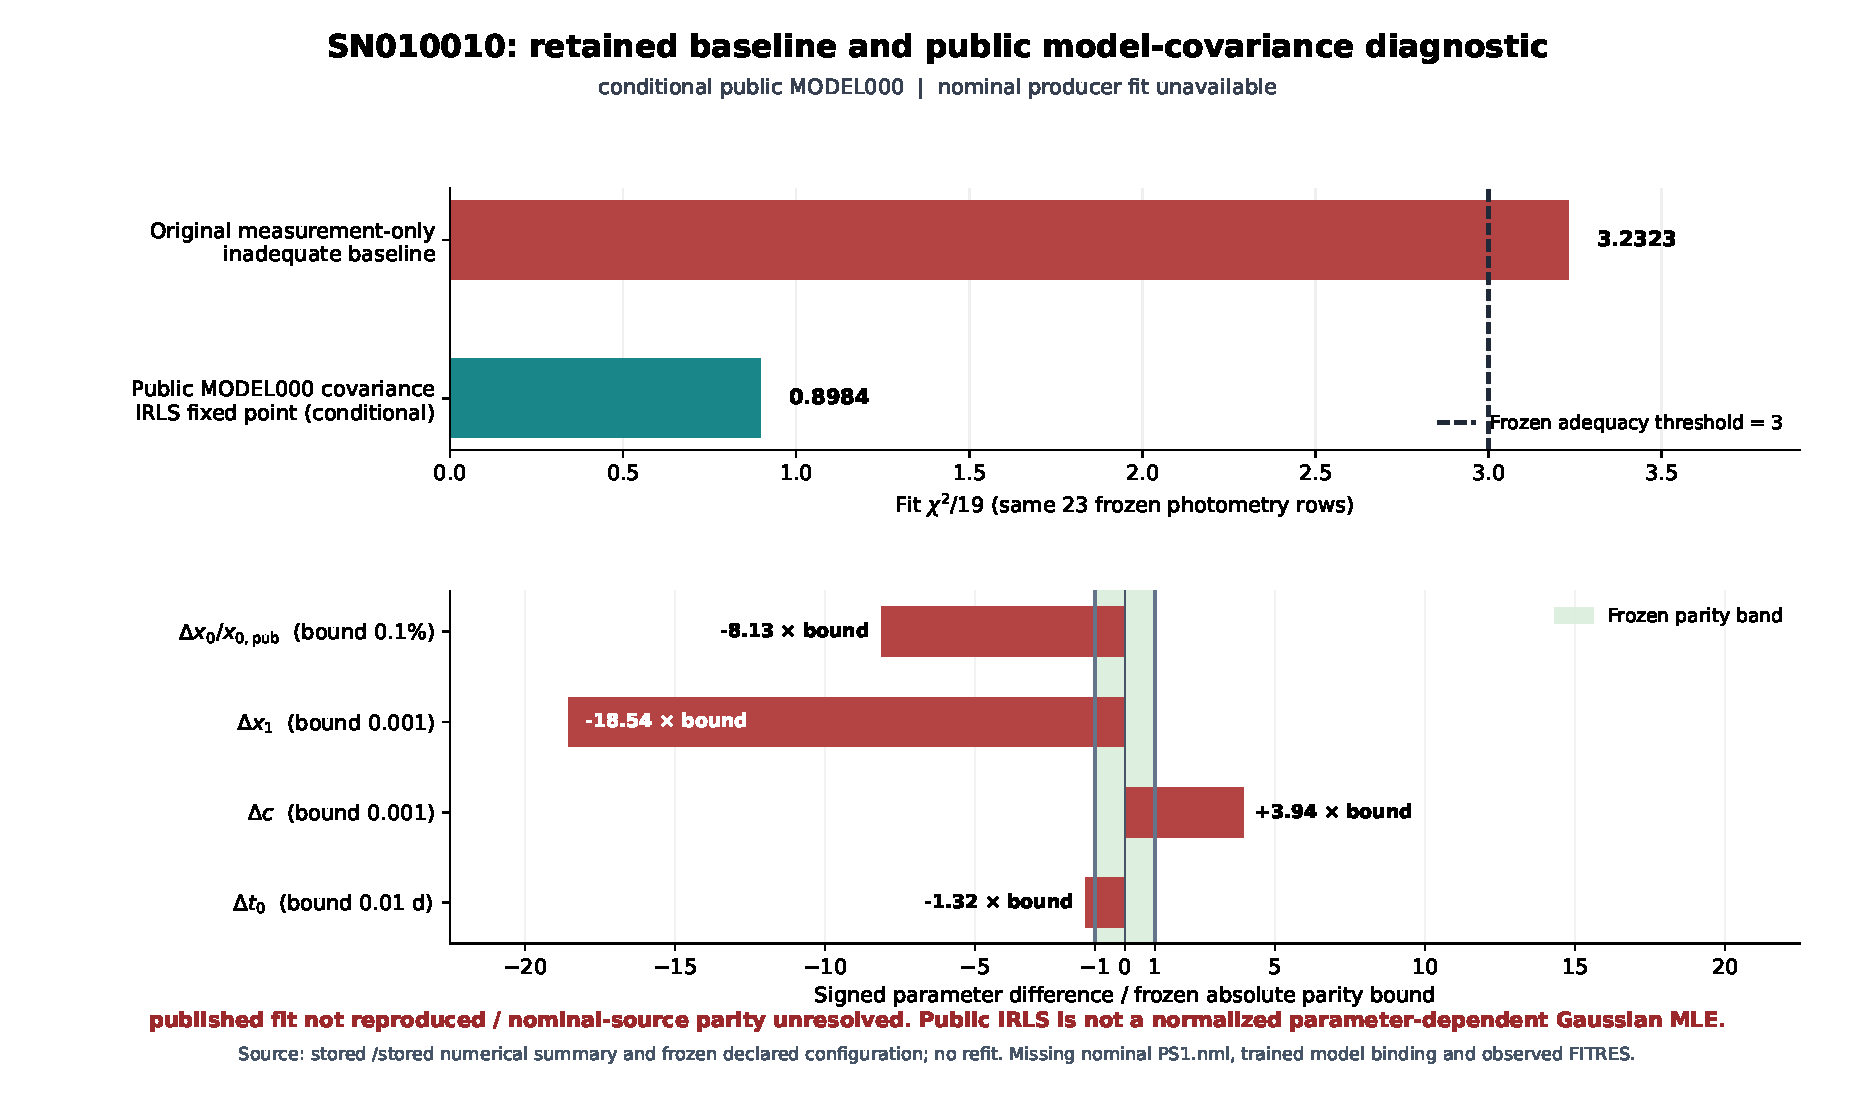
\includegraphics[width=\linewidth,height=.71\textheight,keepaspectratio]{figures/f043_external.pdf}
\caption{SN010010 baseline and public model-covariance comparison. The covariance lowers the conditional residual quadratic, but all stated nominal-summary parity screens fail. The iterated fixed-covariance solution is not the nominal producer fit or a parameter-dependent Gaussian maximum-likelihood fit.}
\label{fig:f043}
\end{figure}
\clearpage
\begin{figure}[p]
\centering
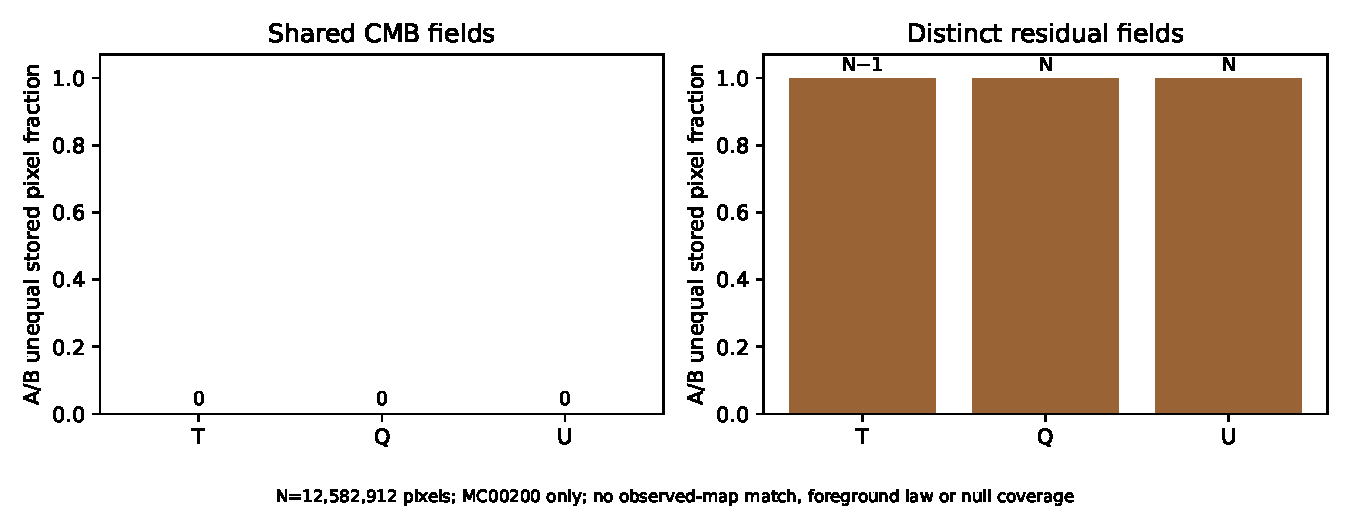
\includegraphics[width=\linewidth,height=.71\textheight,keepaspectratio]{figures/f044.pdf}
\caption{One retained Planck PR4 simulation quartet. Shared CMB fields and distinct residual fields are checked at their original pixels. Identity of the common field is not a joint half-mission source-law qualification or an ensemble noise-covariance estimate.}
\label{fig:f044}
\end{figure}
\clearpage
\begin{figure}[p]
\centering
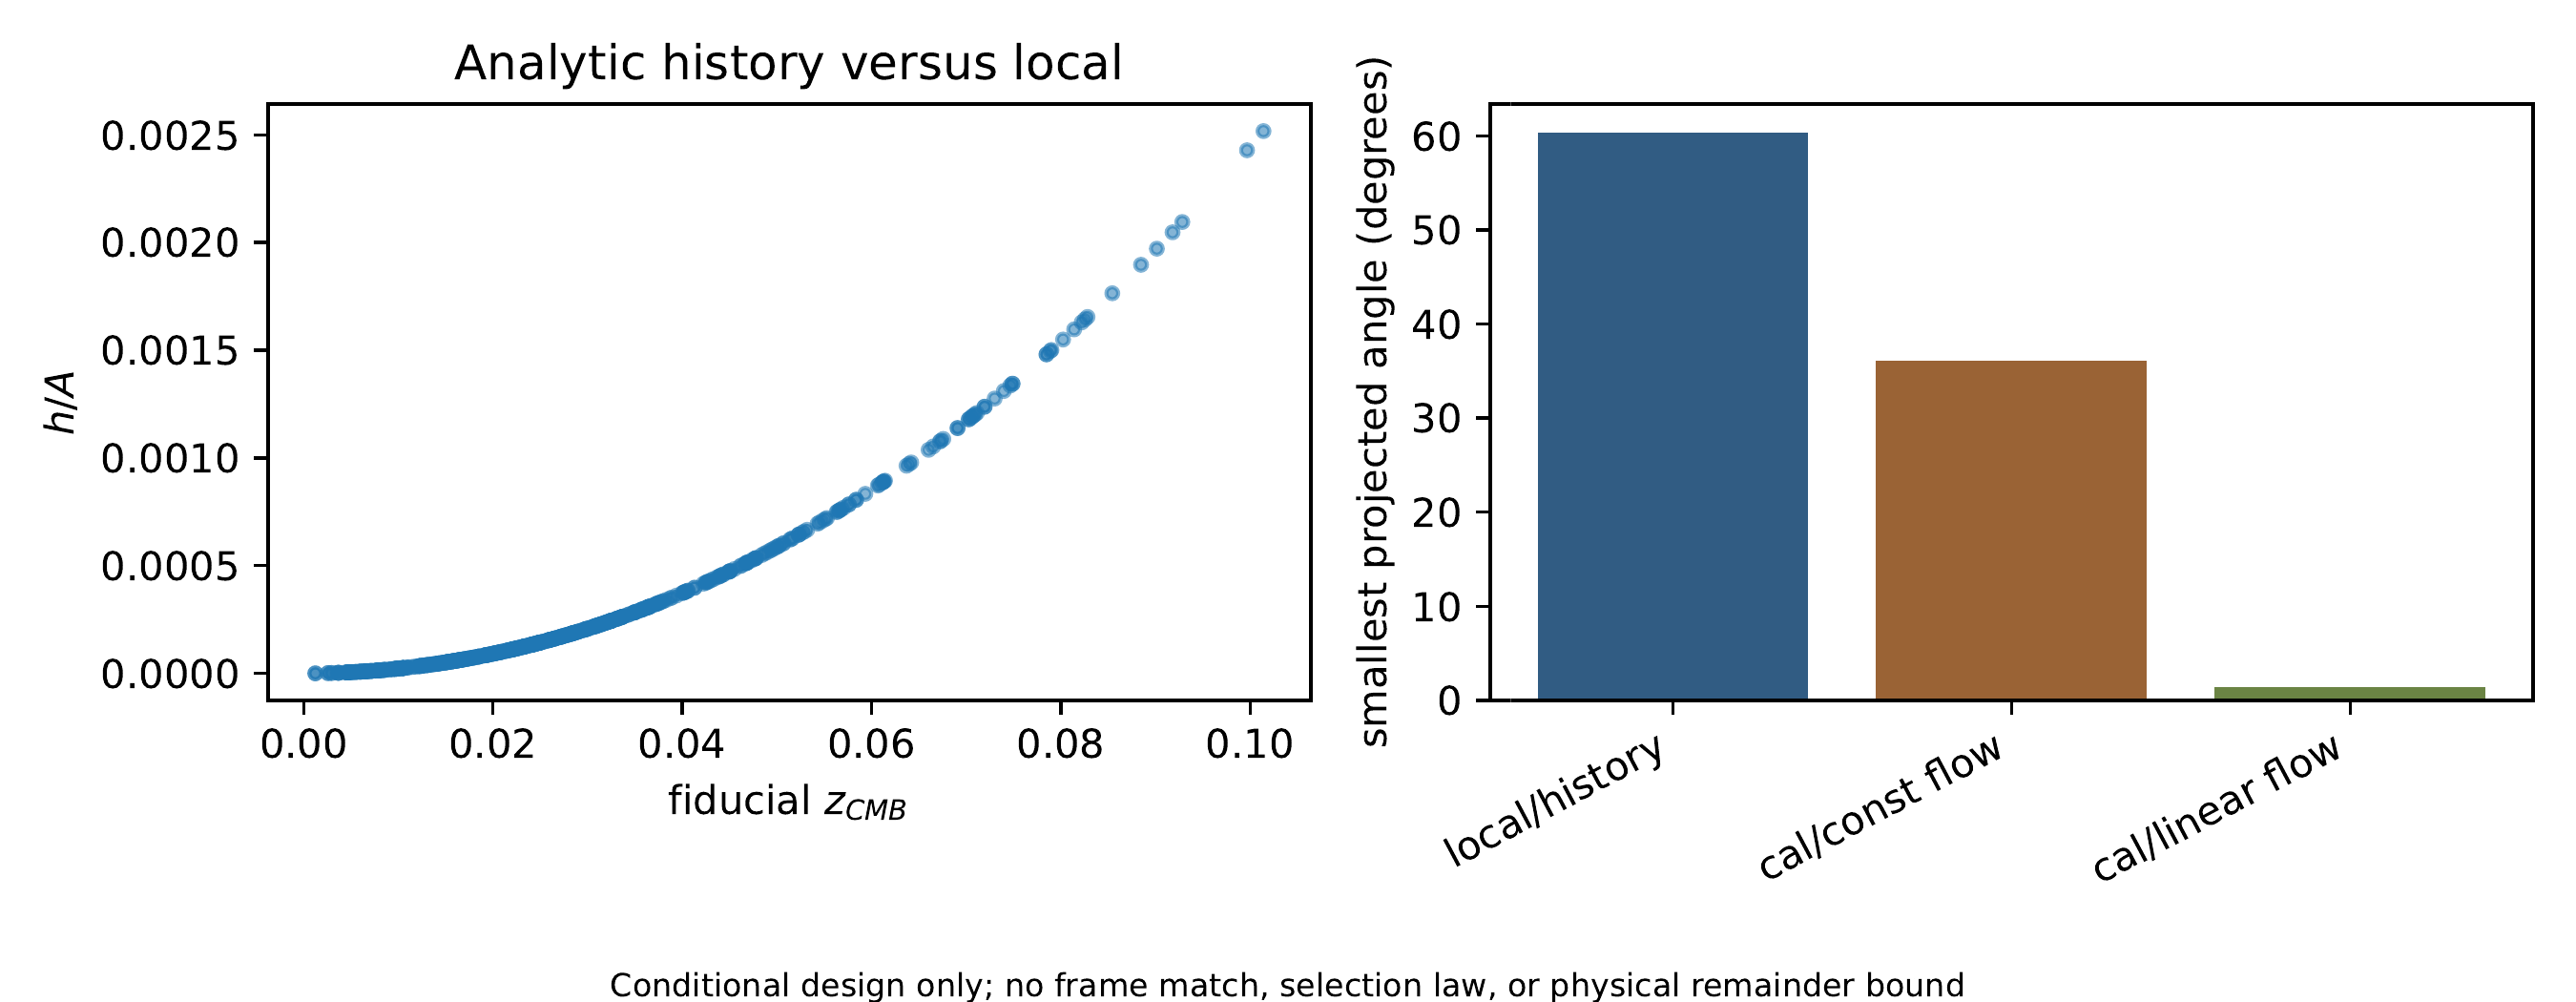
\includegraphics[width=\linewidth,height=.71\textheight,keepaspectratio]{figures/f045_external.png}
\caption{Nuisance-projected response geometry for the retained Pantheon+ and Cosmicflows comparison. The angular and distance-response columns have different principal-angle separation after the specified calibration and dipole projections. The plotted source geometry is conditional on those columns and weights; it does not establish the physical response, joint covariance, or useful discrimination power.}
\label{fig:f045}
\end{figure}
\clearpage
\begin{figure}[p]
\centering
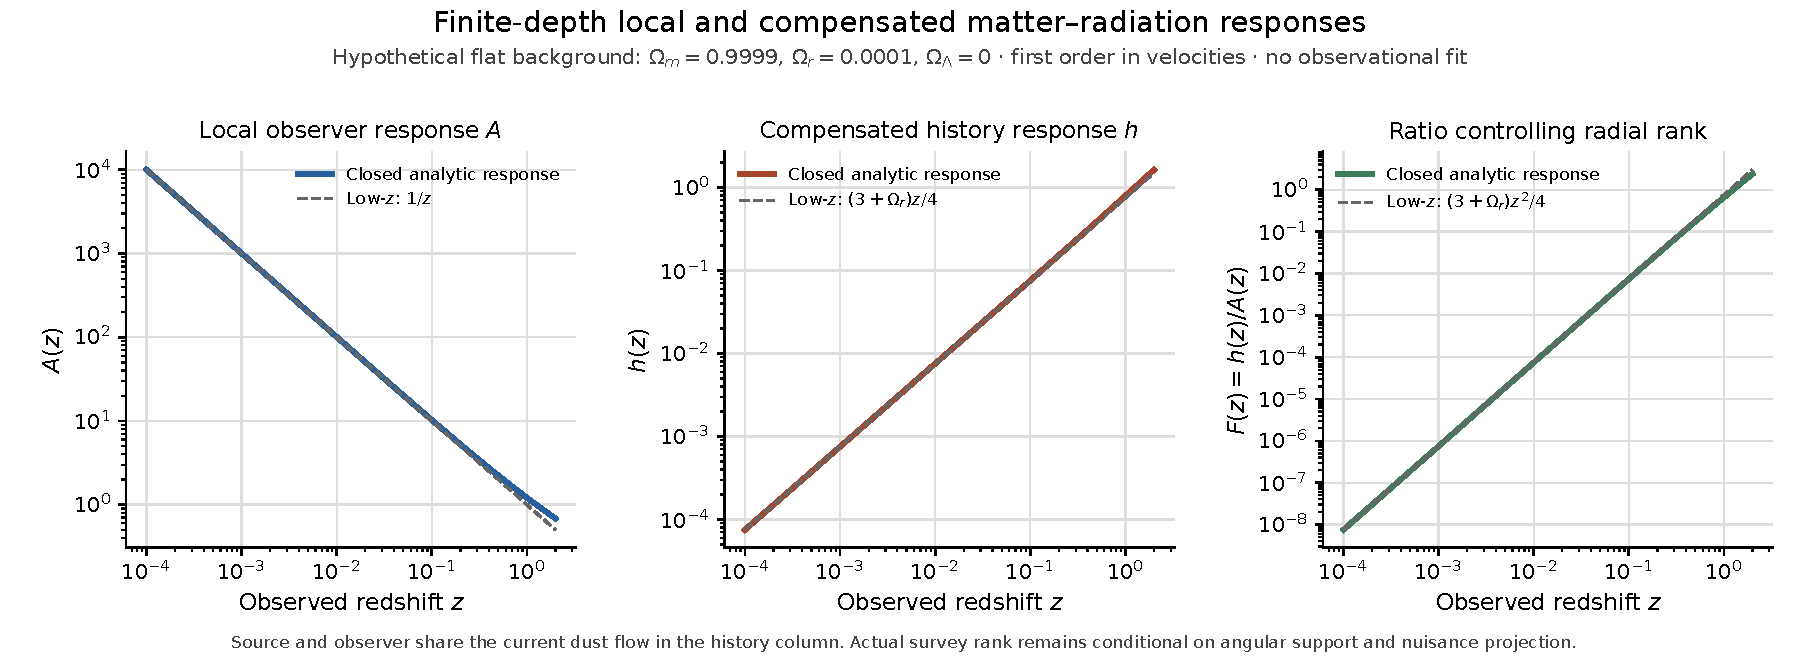
\includegraphics[width=\linewidth,height=.71\textheight,keepaspectratio]{figures/f046.pdf}
\caption{Analytic local-observer and compensated matter--radiation responses in a specified hypothetical background, to first order in velocities. Nonproportional depth dependence can permit conditional discrimination. No observational fit, finite-redshift remainder measurement, or general cosmological response follows.}
\label{fig:f046}
\end{figure}
\clearpage
\begin{figure}[p]
\centering
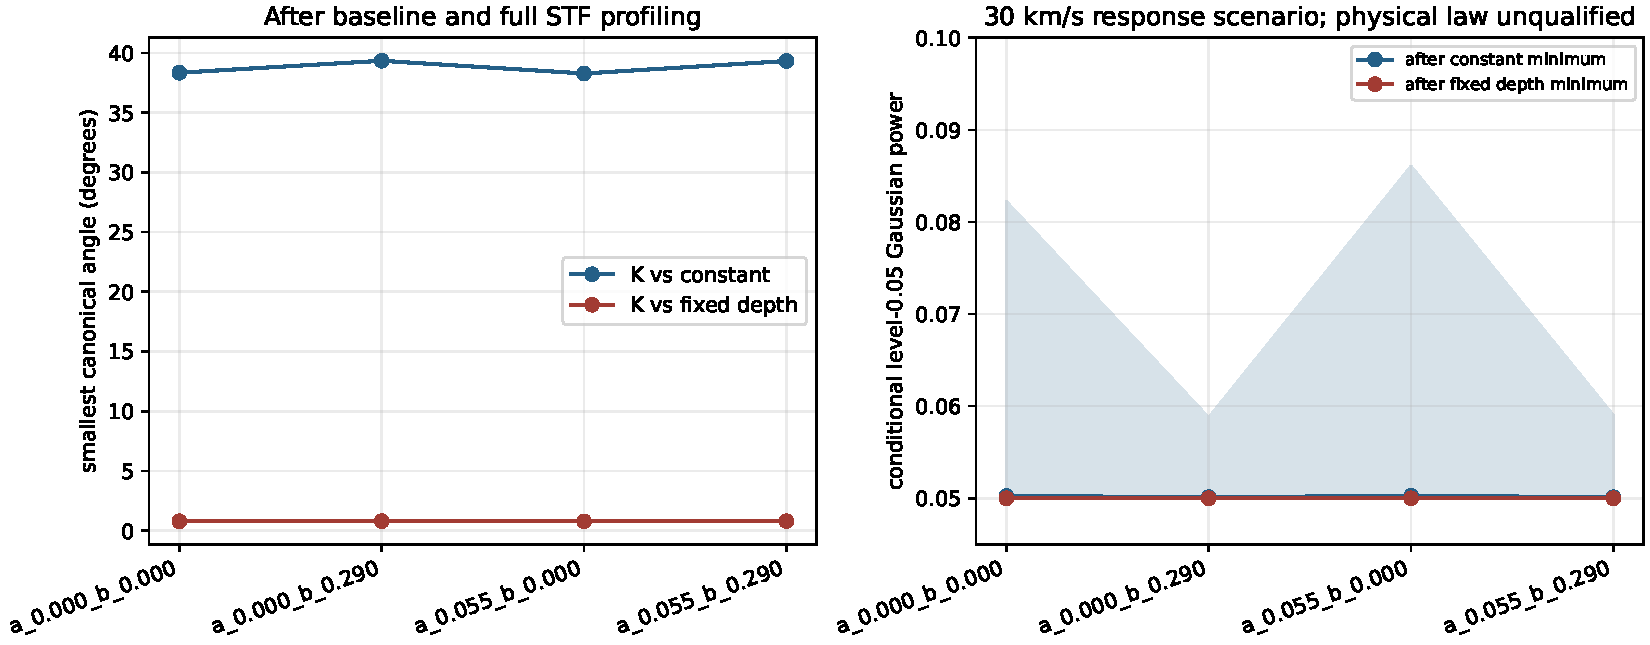
\includegraphics[width=\linewidth,height=.71\textheight,keepaspectratio]{figures/f047_external.pdf}
\caption{Geometry and conditional power of inverse-velocity, constant-calibration, and polynomial-depth vector responses on the retained distance cohort. The broader depth nuisance nearly absorbs the inverse-velocity response. These are selected-design calculations; the low-speed physical expansion and acceleration interpretation remain unqualified.}
\label{fig:f047}
\end{figure}
\clearpage
\begin{figure}[p]
\centering
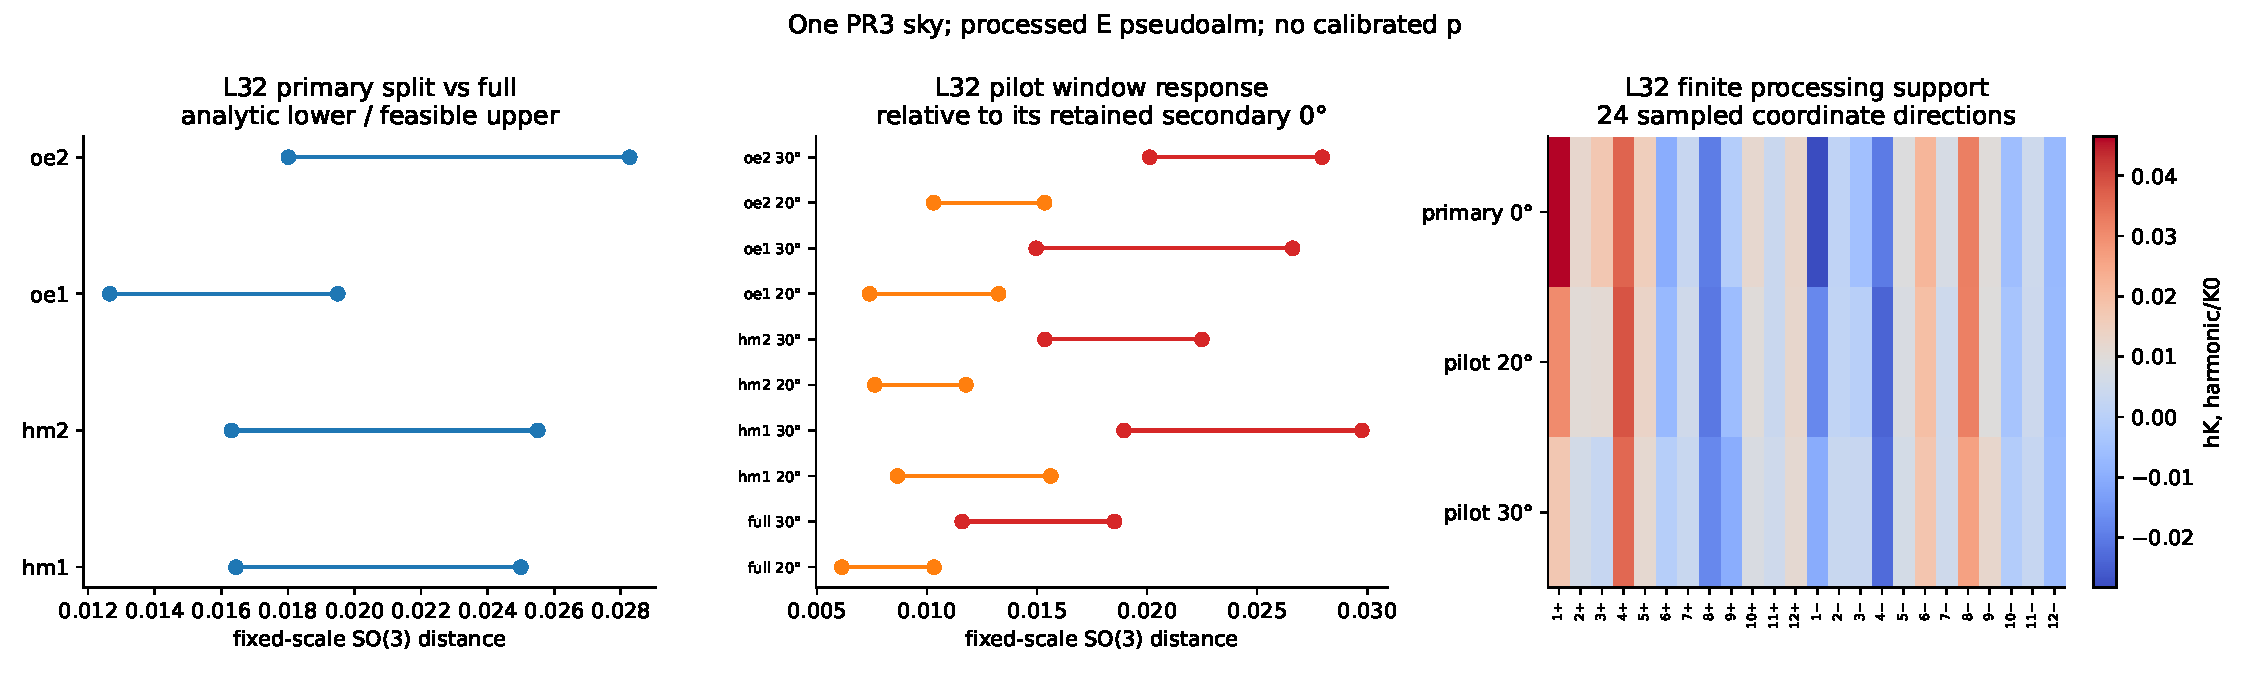
\includegraphics[width=\linewidth,height=.71\textheight,keepaspectratio]{figures/f050_external.pdf}
\caption{Proper-rotation orbit enclosures and sampled directional supports for the complete processed E quadrupole and octupole of one Planck sky. Lower bounds use invariants; upper bounds use feasible rotations. The finite supports describe convex-hull projections, not a physical confidence set or complete nonconvex morphology.}
\label{fig:f050}
\end{figure}
\clearpage
\begin{figure}[p]
\centering
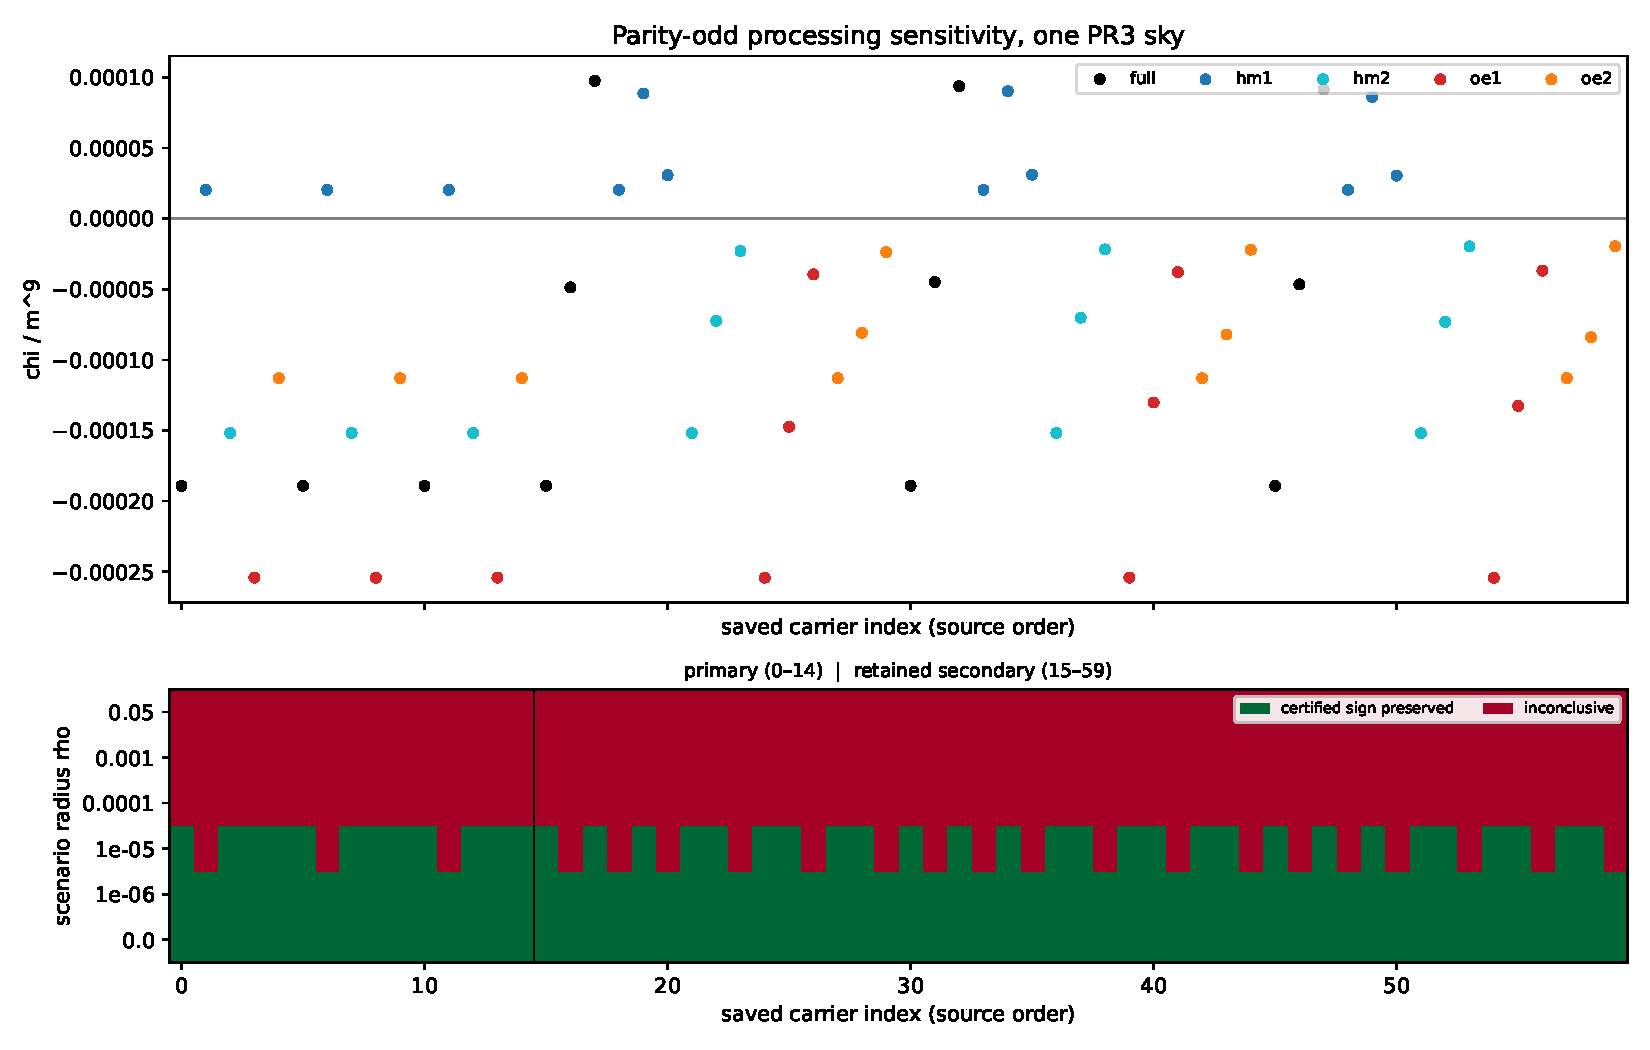
\includegraphics[width=\linewidth,height=.71\textheight,keepaspectratio]{figures/f051_external.pdf}
\caption{Proper-rotation chirality of sixty exact finite processed E tensor carriers and its sensitivity to declared tensor radii. Nonzero signs distinguish each stored carrier from its mirror under proper rotations. The radii are not measured errors, and no primordial parity violation or null significance is inferred.}
\label{fig:f051}
\end{figure}
\clearpage
\begin{figure}[p]
\centering
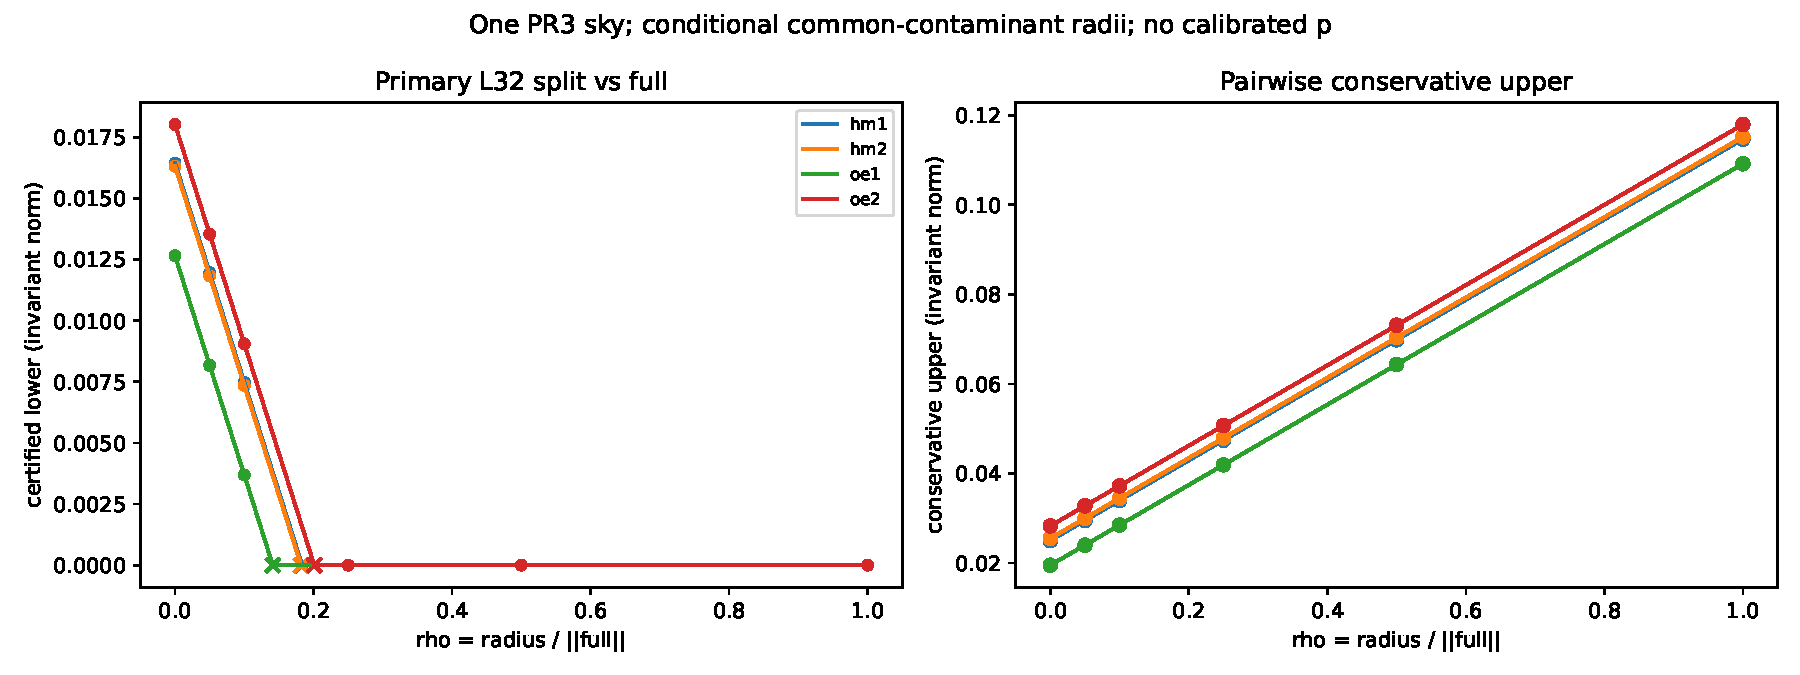
\includegraphics[width=\linewidth,height=.71\textheight,keepaspectratio]{figures/f052.pdf}
\caption{Conservative orbit-distance widening under common-contaminant radius scenarios. A lower certificate reaching zero means that this certificate no longer discriminates. It does not prove equality of the true tensors; common contamination and split cross-noise are not calibrated.}
\label{fig:f052}
\end{figure}
\clearpage
\begin{figure}[p]
\centering
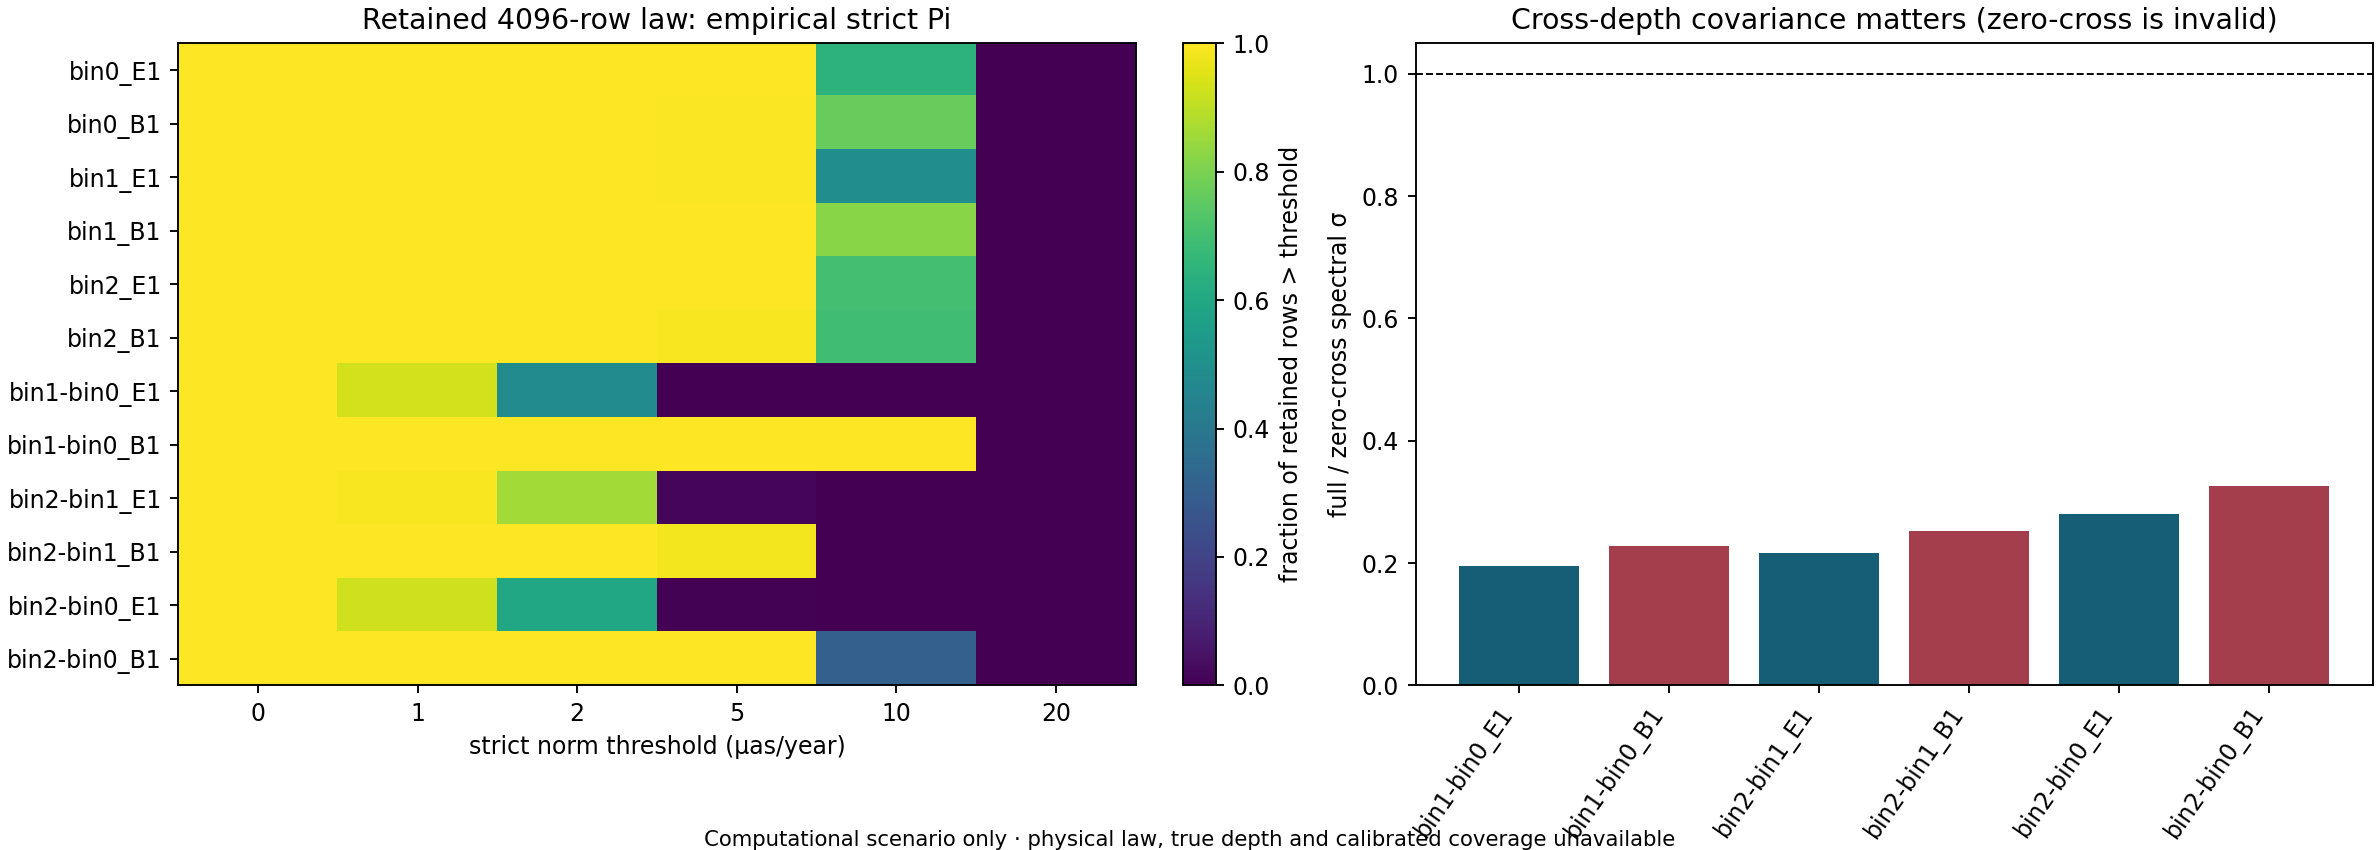
\includegraphics[width=\linewidth,height=.71\textheight,keepaspectratio]{figures/f054.png}
\caption{Strict empirical exceedances and cross-depth covariance effects for the same 4096 joint astrometric rows. The corrected reported-bin map includes the shared slope. Removing covariance is a counterfactual diagnostic; finite frequencies are not physical probabilities.}
\label{fig:f054}
\end{figure}
\clearpage
\begin{figure}[p]
\centering
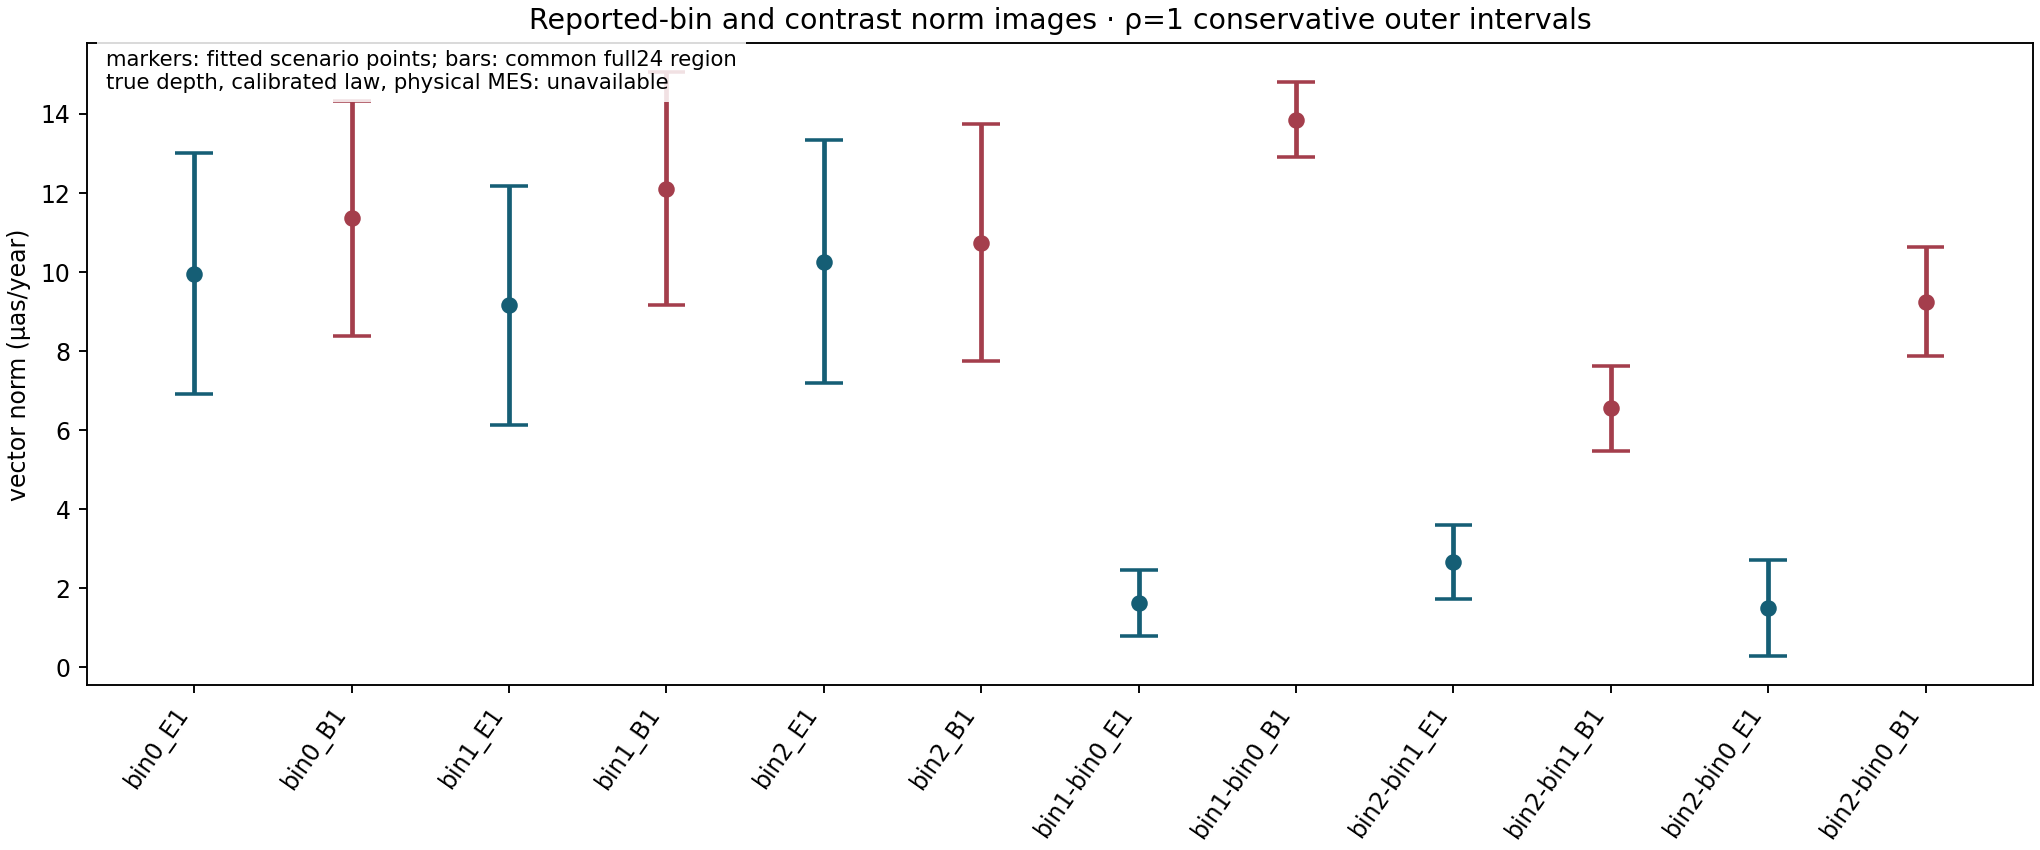
\includegraphics[width=\linewidth,height=.71\textheight,keepaspectratio]{figures/f055.png}
\caption{Full-covariance functional depth images of the astrometric state, with reported-bin values and contrasts. Coordinate support is exact under the declared joint region; norm bars are conservative outer bounds. True-depth response and physical coverage remain unqualified.}
\label{fig:f055}
\end{figure}
\clearpage
\begin{figure}[p]
\centering
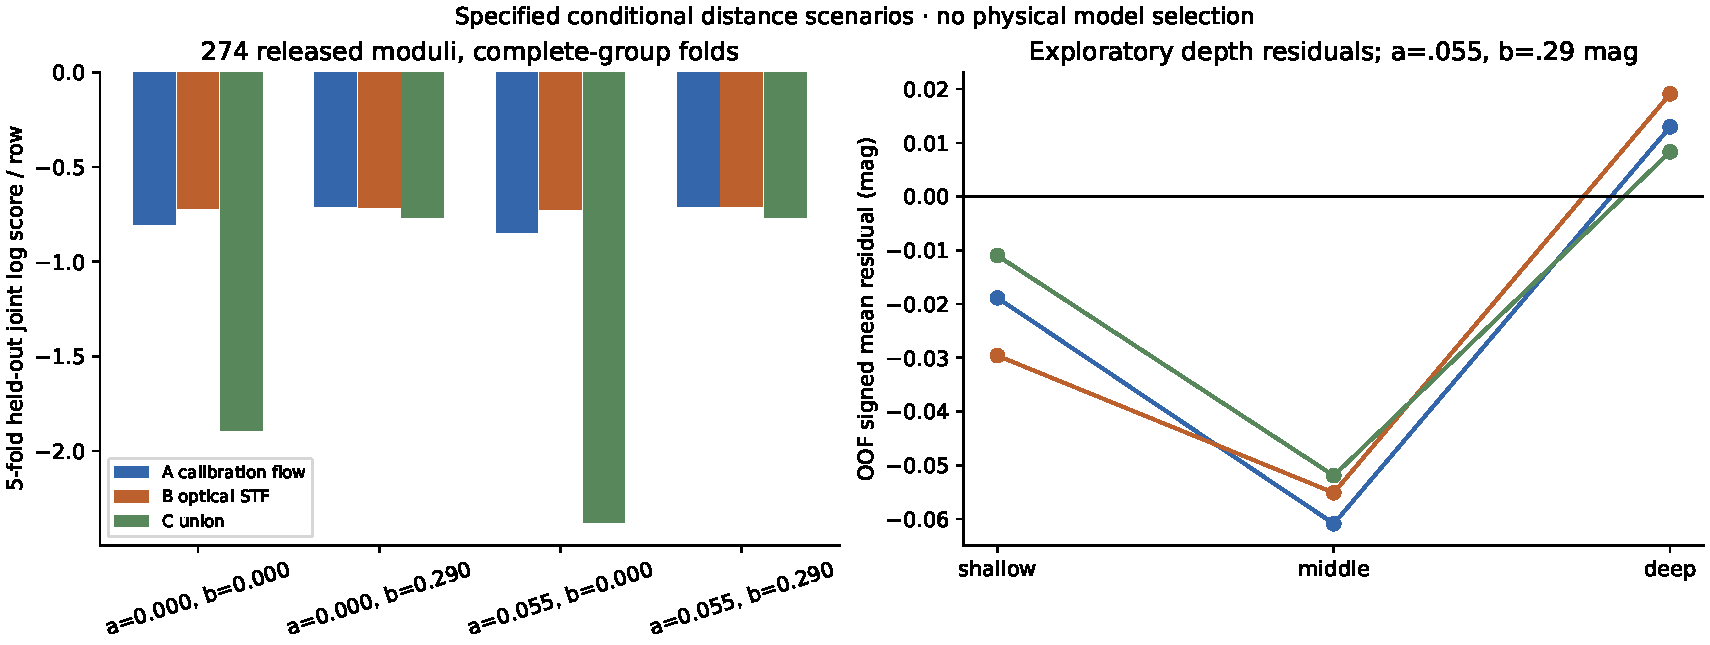
\includegraphics[width=\linewidth,height=.71\textheight,keepaspectratio]{figures/f058_external.pdf}
\caption{Whole-group held-out distance prediction and signed residual summaries. The model ranking changes with the declared group-covariance scenario. All scenarios use the same observed cohort; the plots do not validate a physical calibration, flow, or shear interpretation.}
\label{fig:f058}
\end{figure}
\clearpage
\begin{figure}[p]
\centering
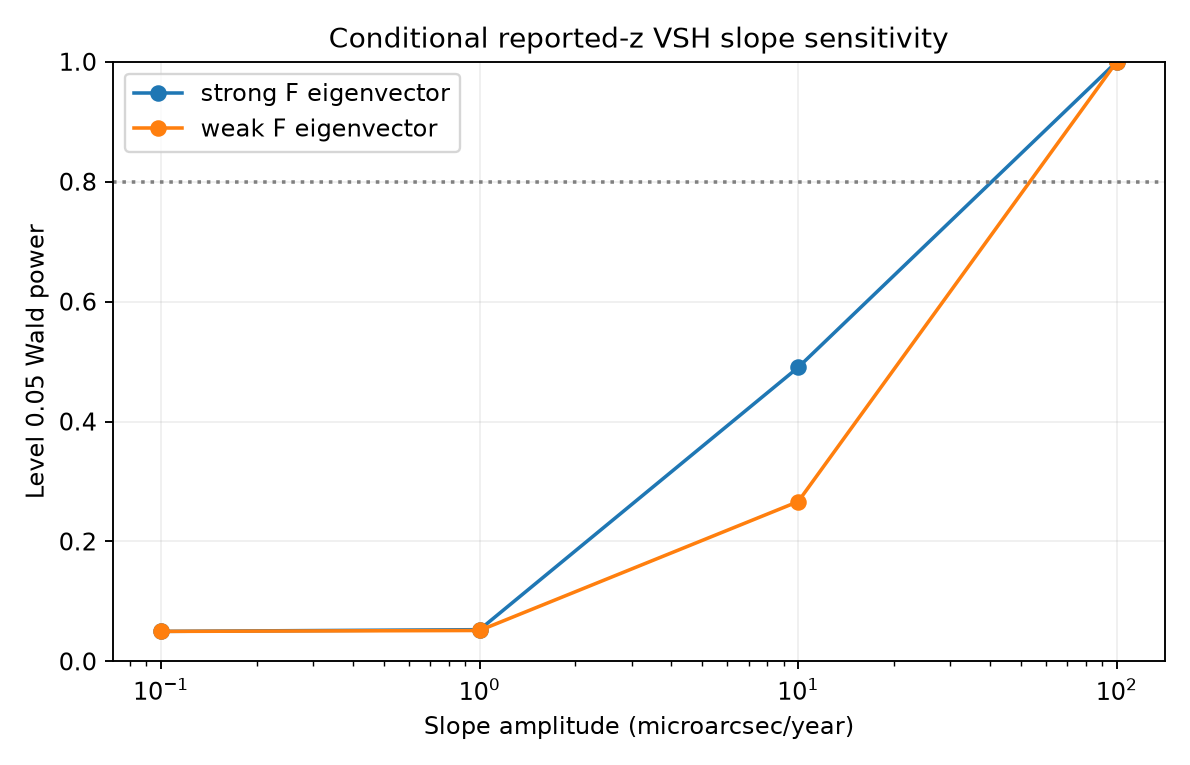
\includegraphics[width=\linewidth,height=.71\textheight,keepaspectratio]{figures/f059.png}
\caption{Continuous reported-redshift slope response after profiling the full astrometric nuisance design. The power curves and errors use the independent-row reported-covariance Gaussian working law. They are conditional design quantities, not empirical physical limits.}
\label{fig:f059}
\end{figure}
\clearpage
\begin{figure}[p]
\centering
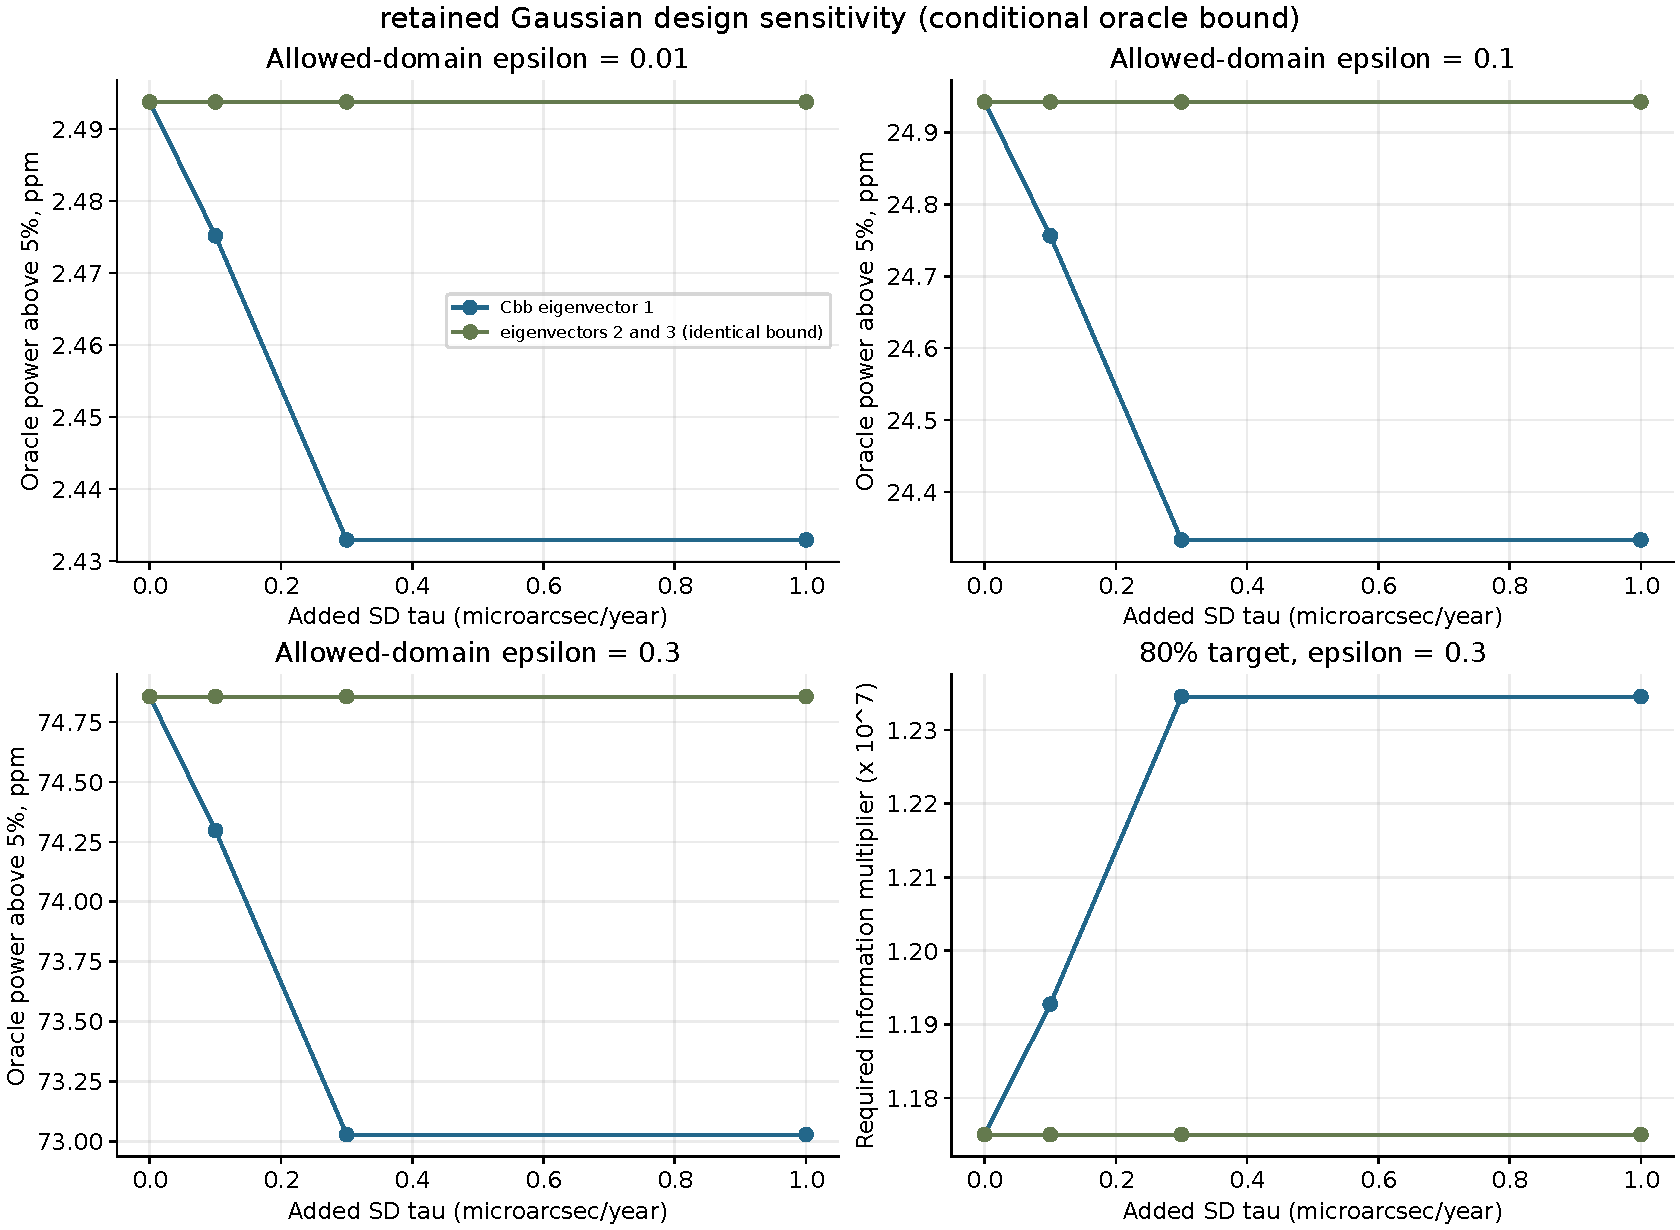
\includegraphics[width=\linewidth,height=.71\textheight,keepaspectratio]{figures/f060_external.pdf}
\caption{Oracle power sensitivity for the retained profiled astrometric history covariance. The allowed-domain parameter and added covariance are scenarios. Information multipliers are requirements within the fixed response model, not demonstrated observing-program improvements.}
\label{fig:f060}
\end{figure}
\clearpage
\begin{figure}[p]
\centering
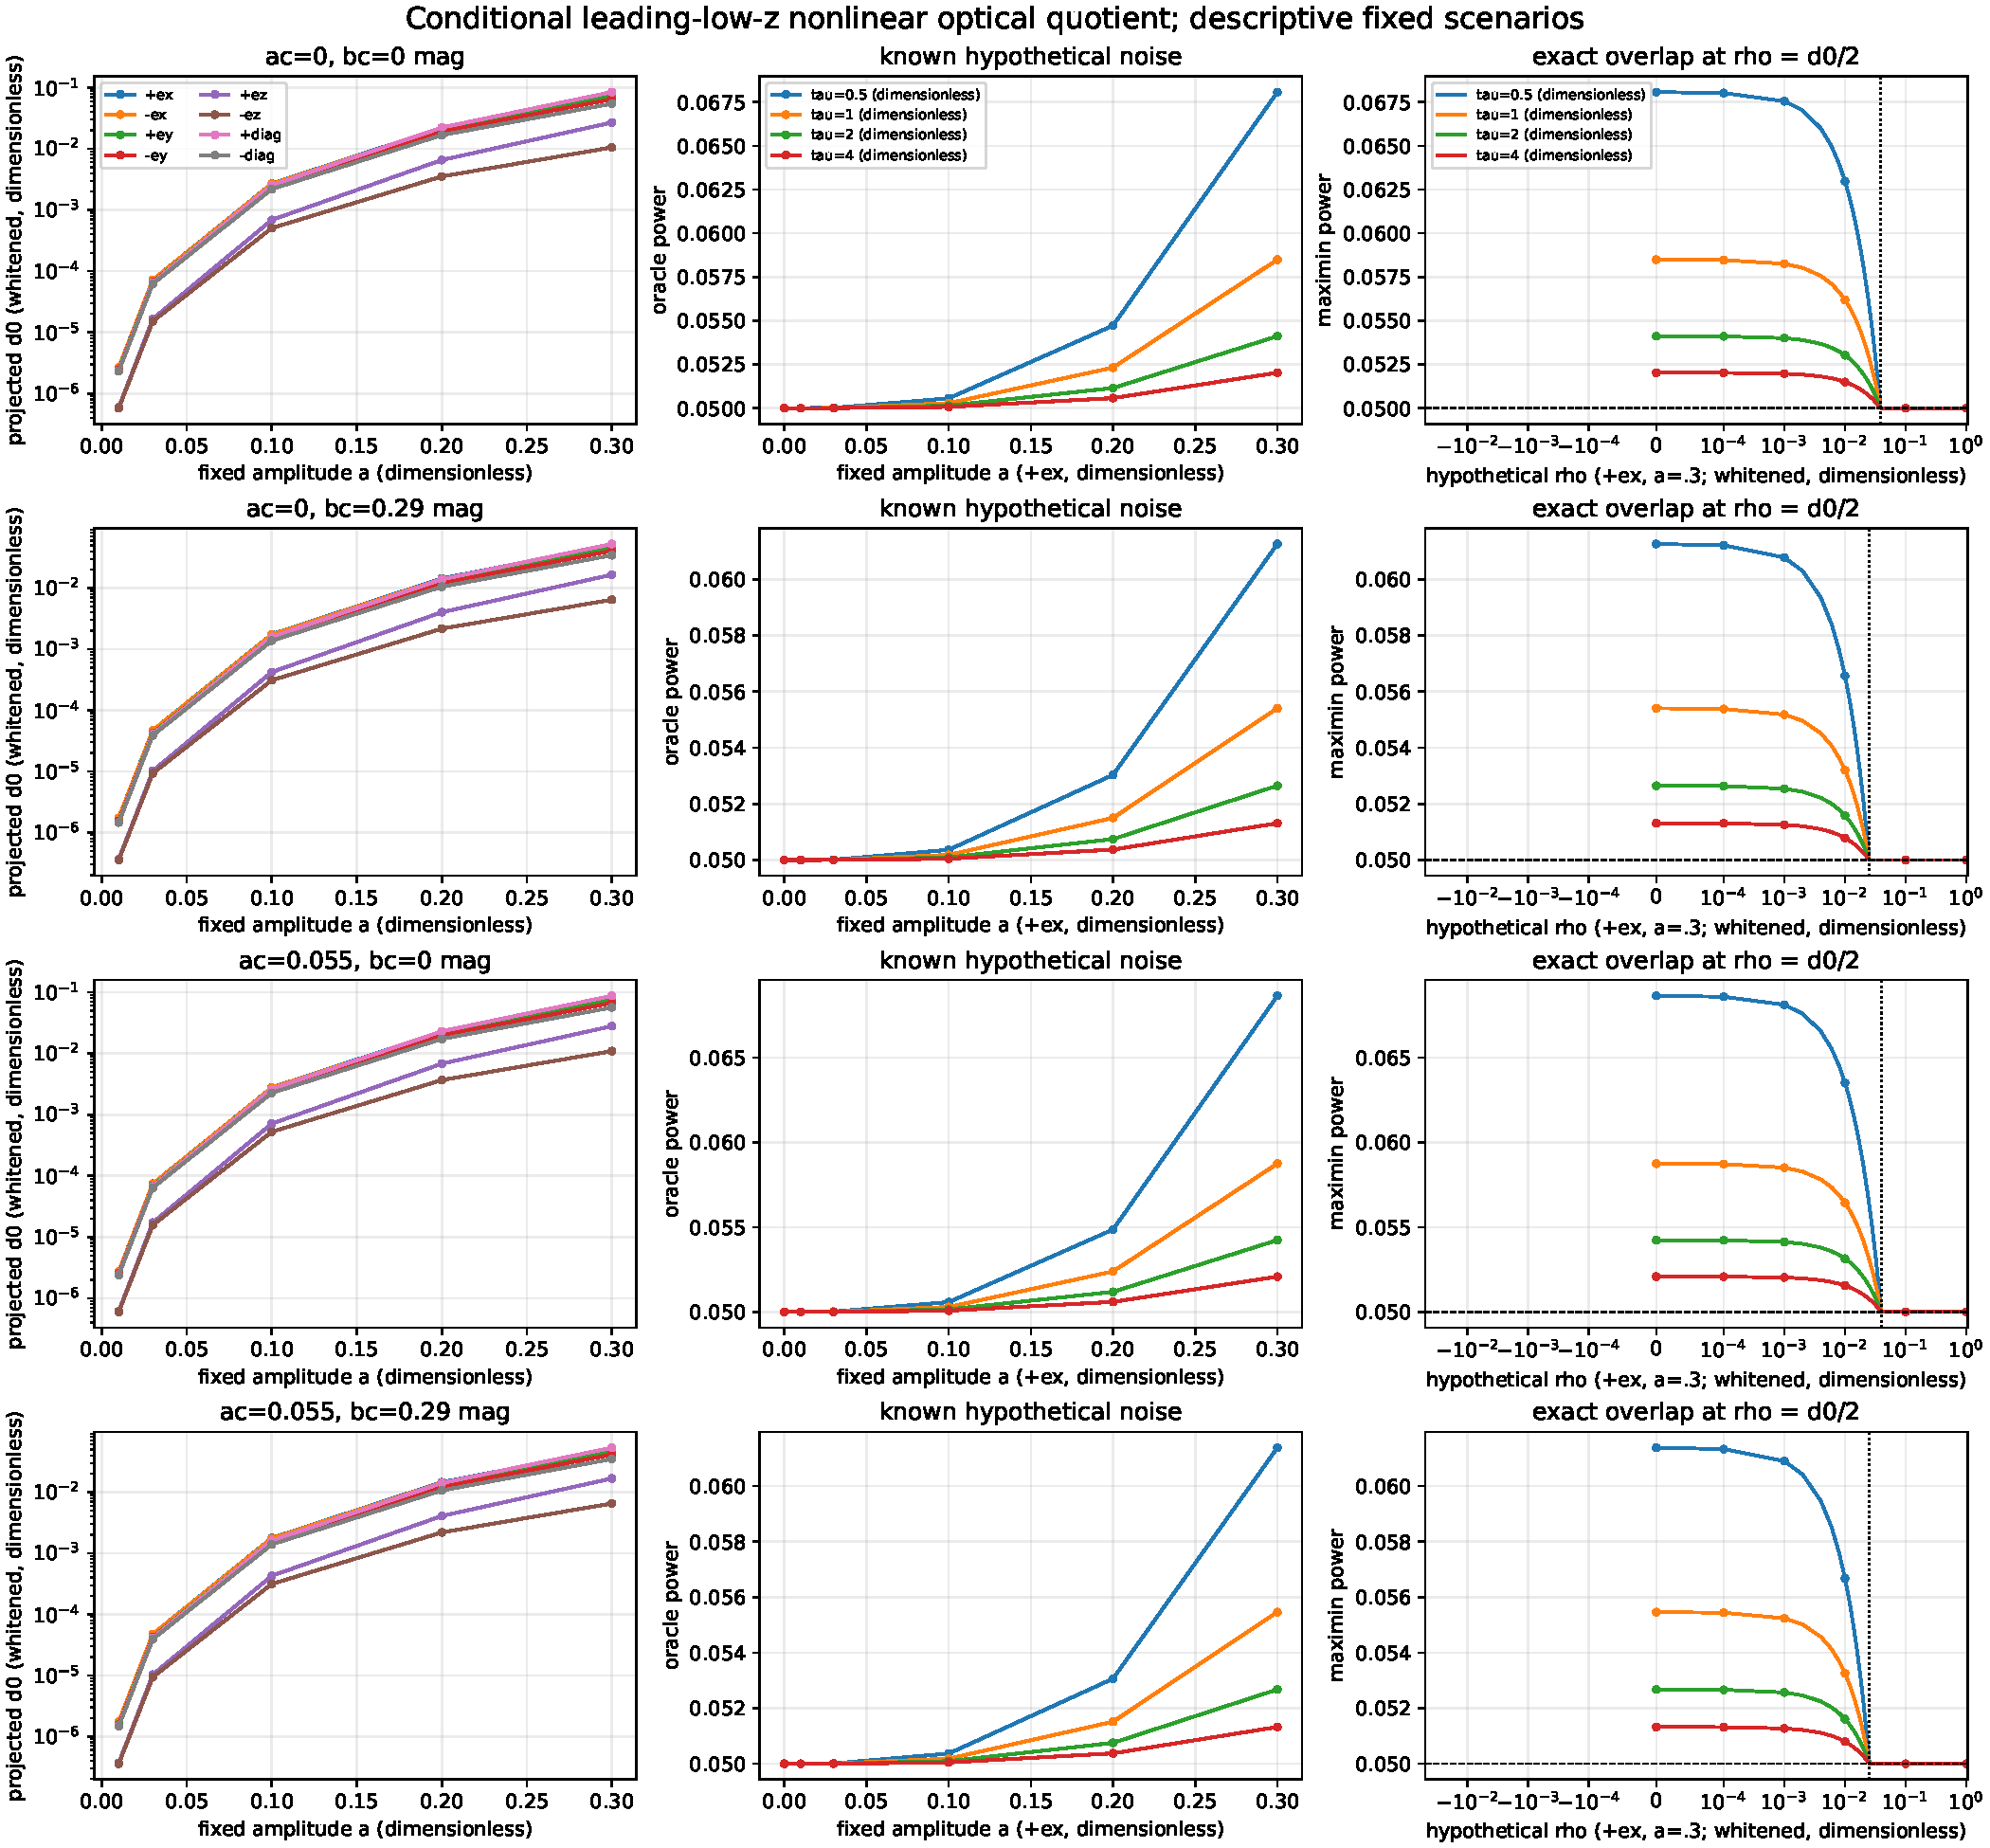
\includegraphics[width=\linewidth,height=.71\textheight,keepaspectratio]{figures/f061.pdf}
\caption{Nonlinear optical response after quotienting the fitted baseline, dipole, and STF space. All directions and amplitudes are fixed scenarios. The remainder curves include the exact overlap radius; beyond overlap the conditional benchmark is the test size. Finite-redshift physical remainder is unmeasured.}
\label{fig:f061}
\end{figure}
\clearpage
\begin{figure}[p]
\centering
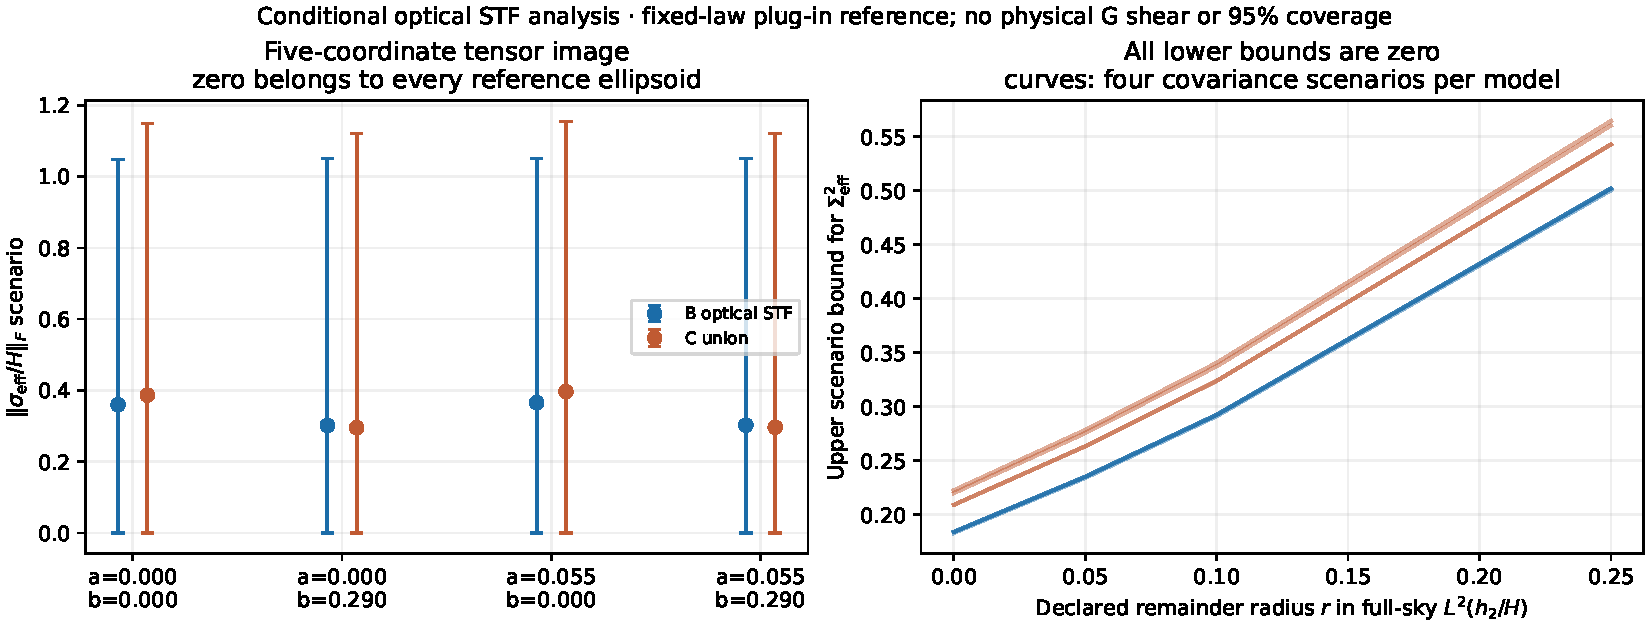
\includegraphics[width=\linewidth,height=.71\textheight,keepaspectratio]{figures/f063.pdf}
\caption{Full-covariance optical STF images of the selected distance fits. Every reference ellipsoid permits zero quadrupole. The effective-shear conversion is a linearized fixed-redshift scenario; its reference region and added remainder radii do not measure local congruence shear or physical coverage.}
\label{fig:f063}
\end{figure}
\clearpage
\begin{figure}[p]
\centering
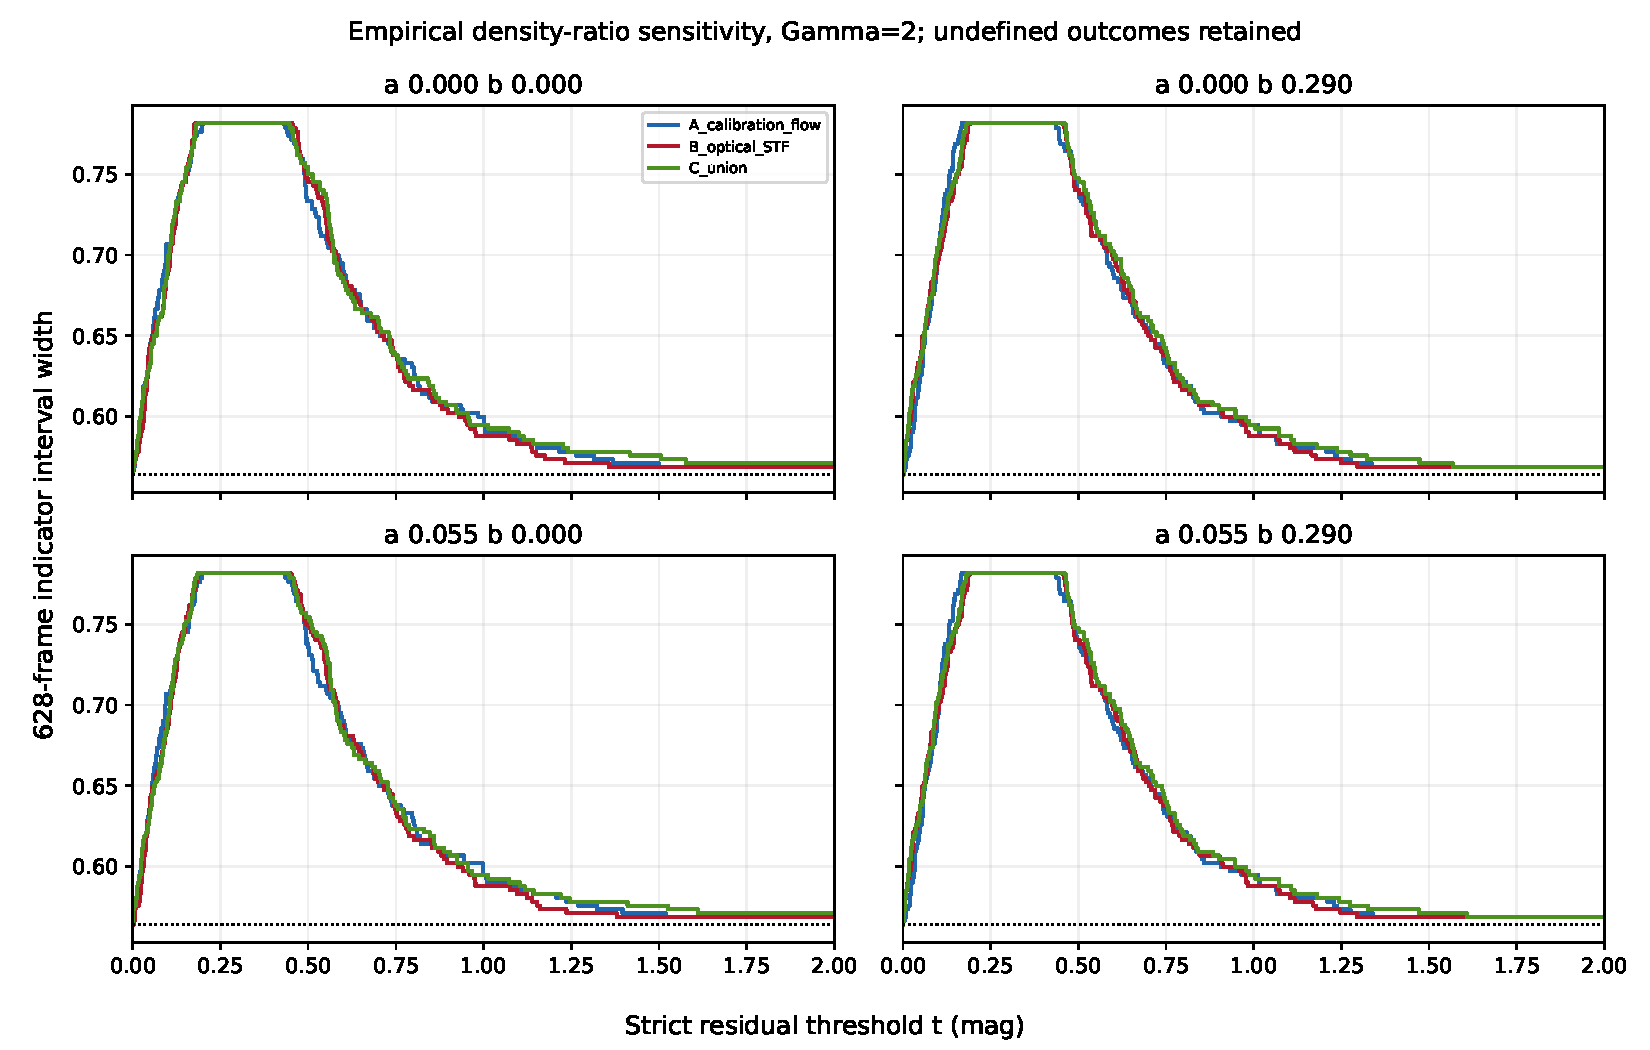
\includegraphics[width=\linewidth,height=.71\textheight,keepaspectratio]{figures/f064.pdf}
\caption{Sharp empirical density-ratio sensitivity followed by unrestricted completion of missing target events. The total interval width retains the missing fraction. These are finite-target event bounds, not estimated parent propensities or a probability of cosmological geometry.}
\label{fig:f064}
\end{figure}
\clearpage
\begin{figure}[p]
\centering
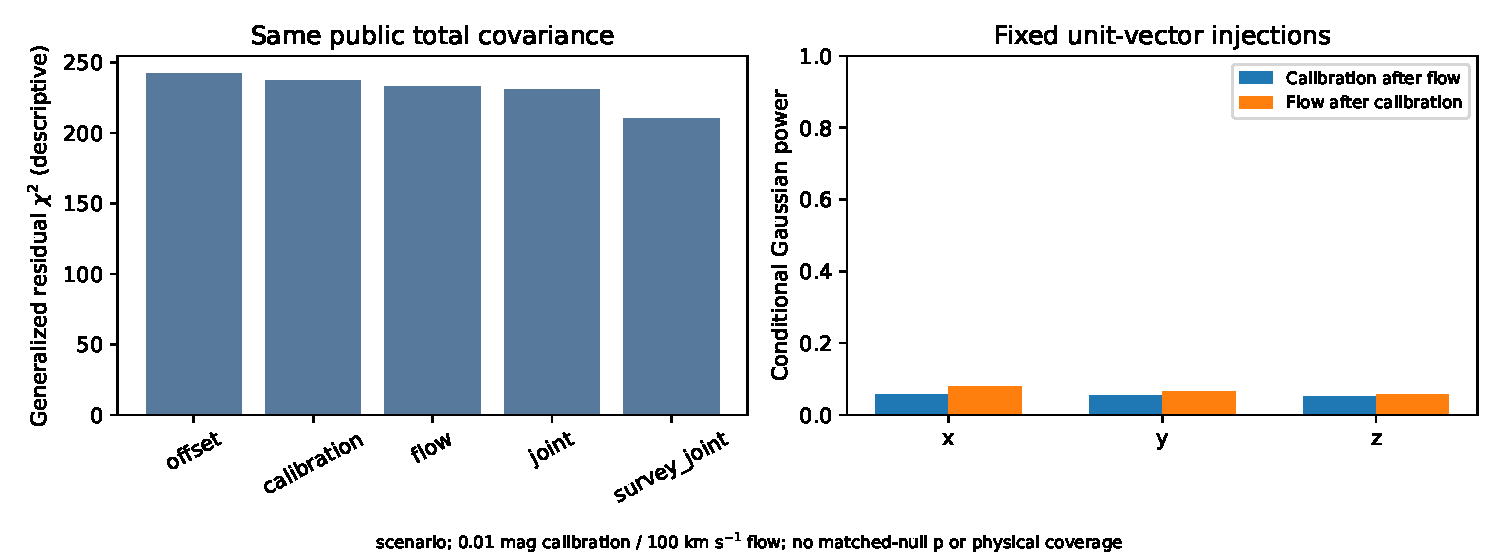
\includegraphics[width=\linewidth,height=.71\textheight,keepaspectratio]{figures/f065_external.pdf}
\caption{Pantheon+ conditional mean-model comparison using the released total covariance once. The residual quadratics are descriptive, and the injection powers use a fixed Gaussian reference. Calibration and frozen-flow coefficient blocks remain correlated; nominal-source parity and cross-survey covariance are not supplied.}
\label{fig:f065}
\end{figure}
\clearpage
\begin{figure}[p]
\centering
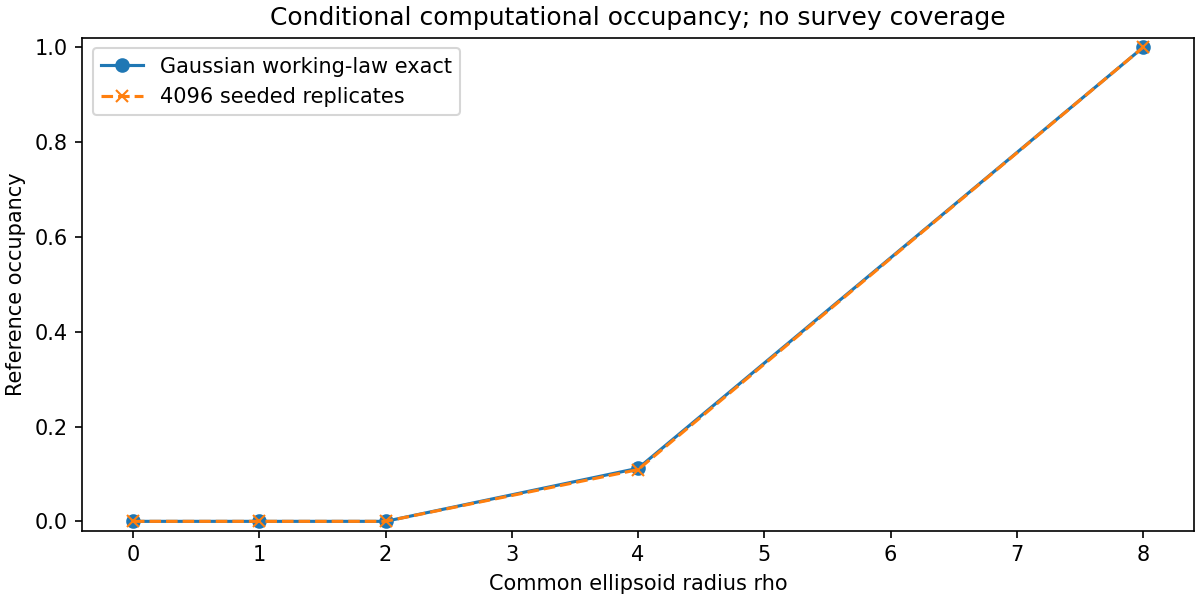
\includegraphics[width=\linewidth,height=.71\textheight,keepaspectratio]{figures/f066.png}
\caption{Occupancy of named computational regions under the stated Gaussian reference and retained joint samples. A reference region is not itself a probability measure. The computational anchor is separate from an unavailable physical bound; no selected-survey coverage is claimed.}
\label{fig:f066}
\end{figure}
\clearpage
\begin{figure}[p]
\centering
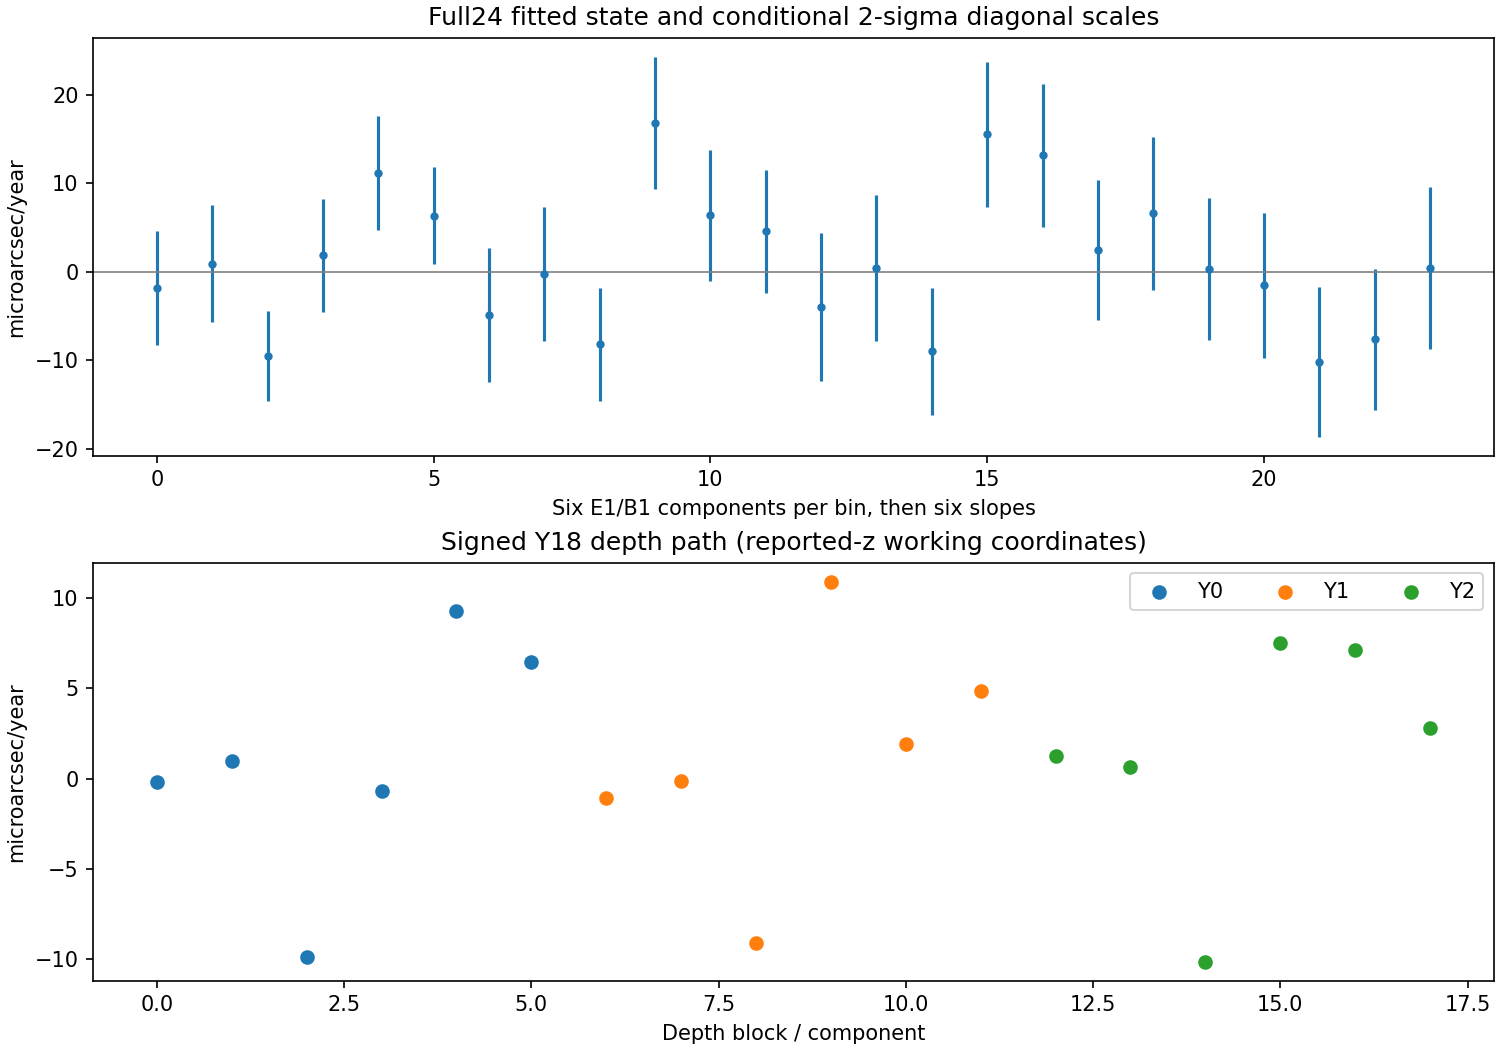
\includegraphics[width=\linewidth,height=.71\textheight,keepaspectratio]{figures/f067.png}
\caption{Full astrometric tensor-state diagnostics with shared covariance and finite empirical exceedance. Polar and axial coordinates and the original state accompany all scalar summaries. The computational norm scale is not a physical anisotropy anchor.}
\label{fig:f067}
\end{figure}
\clearpage
\begin{figure}[p]
\centering
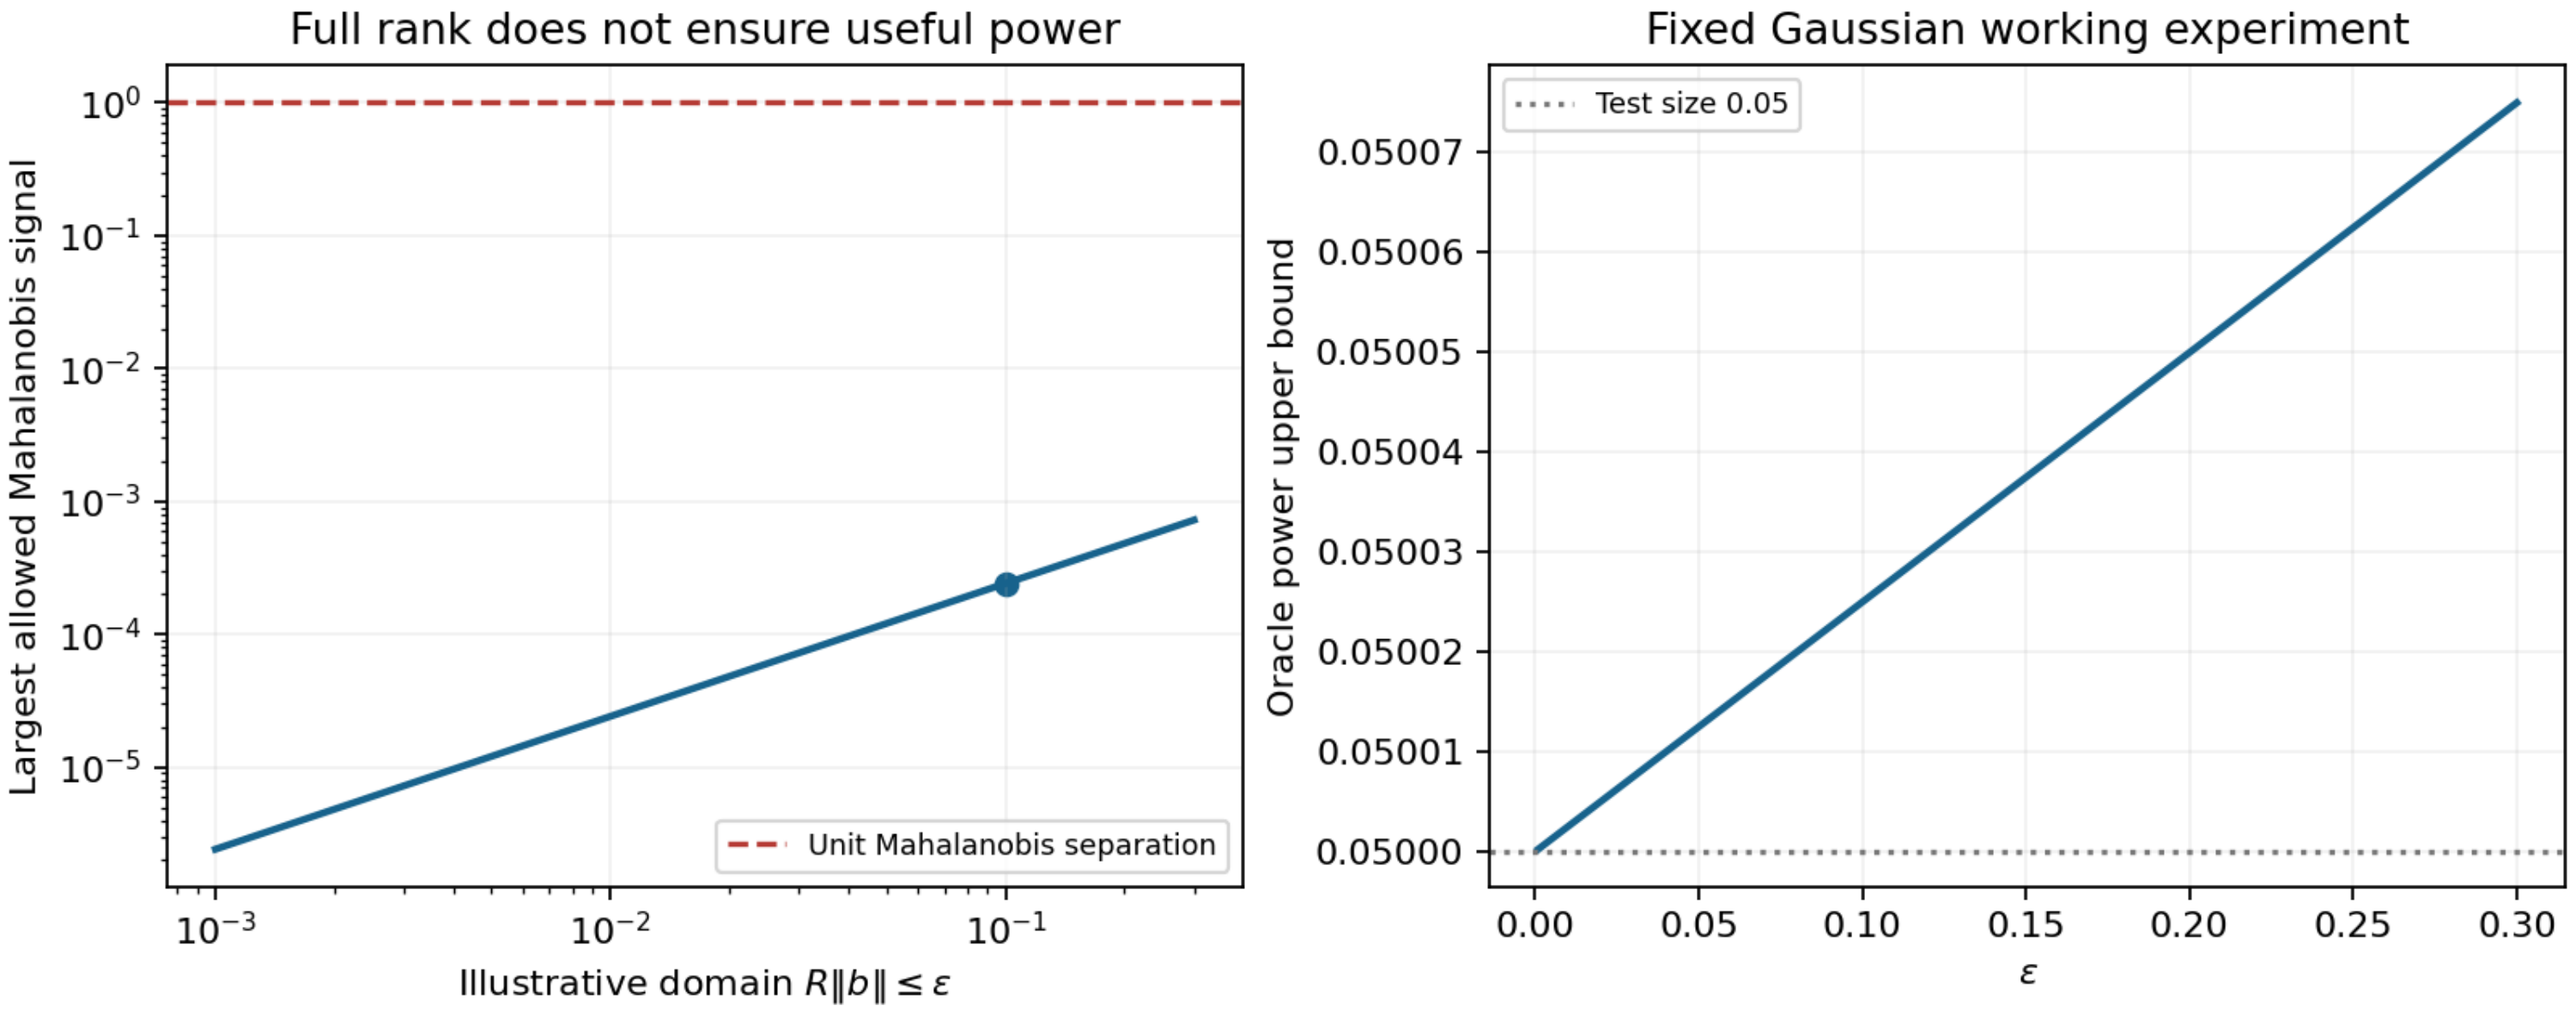
\includegraphics[width=\linewidth,height=.71\textheight,keepaspectratio]{figures/f068_external.png}
\caption{Best-direction Gaussian power in a restricted illustrative history-response domain. Even the oracle bound is close to test size. The restriction controls a stated small parameter; it does not certify every physical remainder or prove a universal observational impossibility.}
\label{fig:f068}
\end{figure}
\clearpage
\begin{figure}[p]
\centering
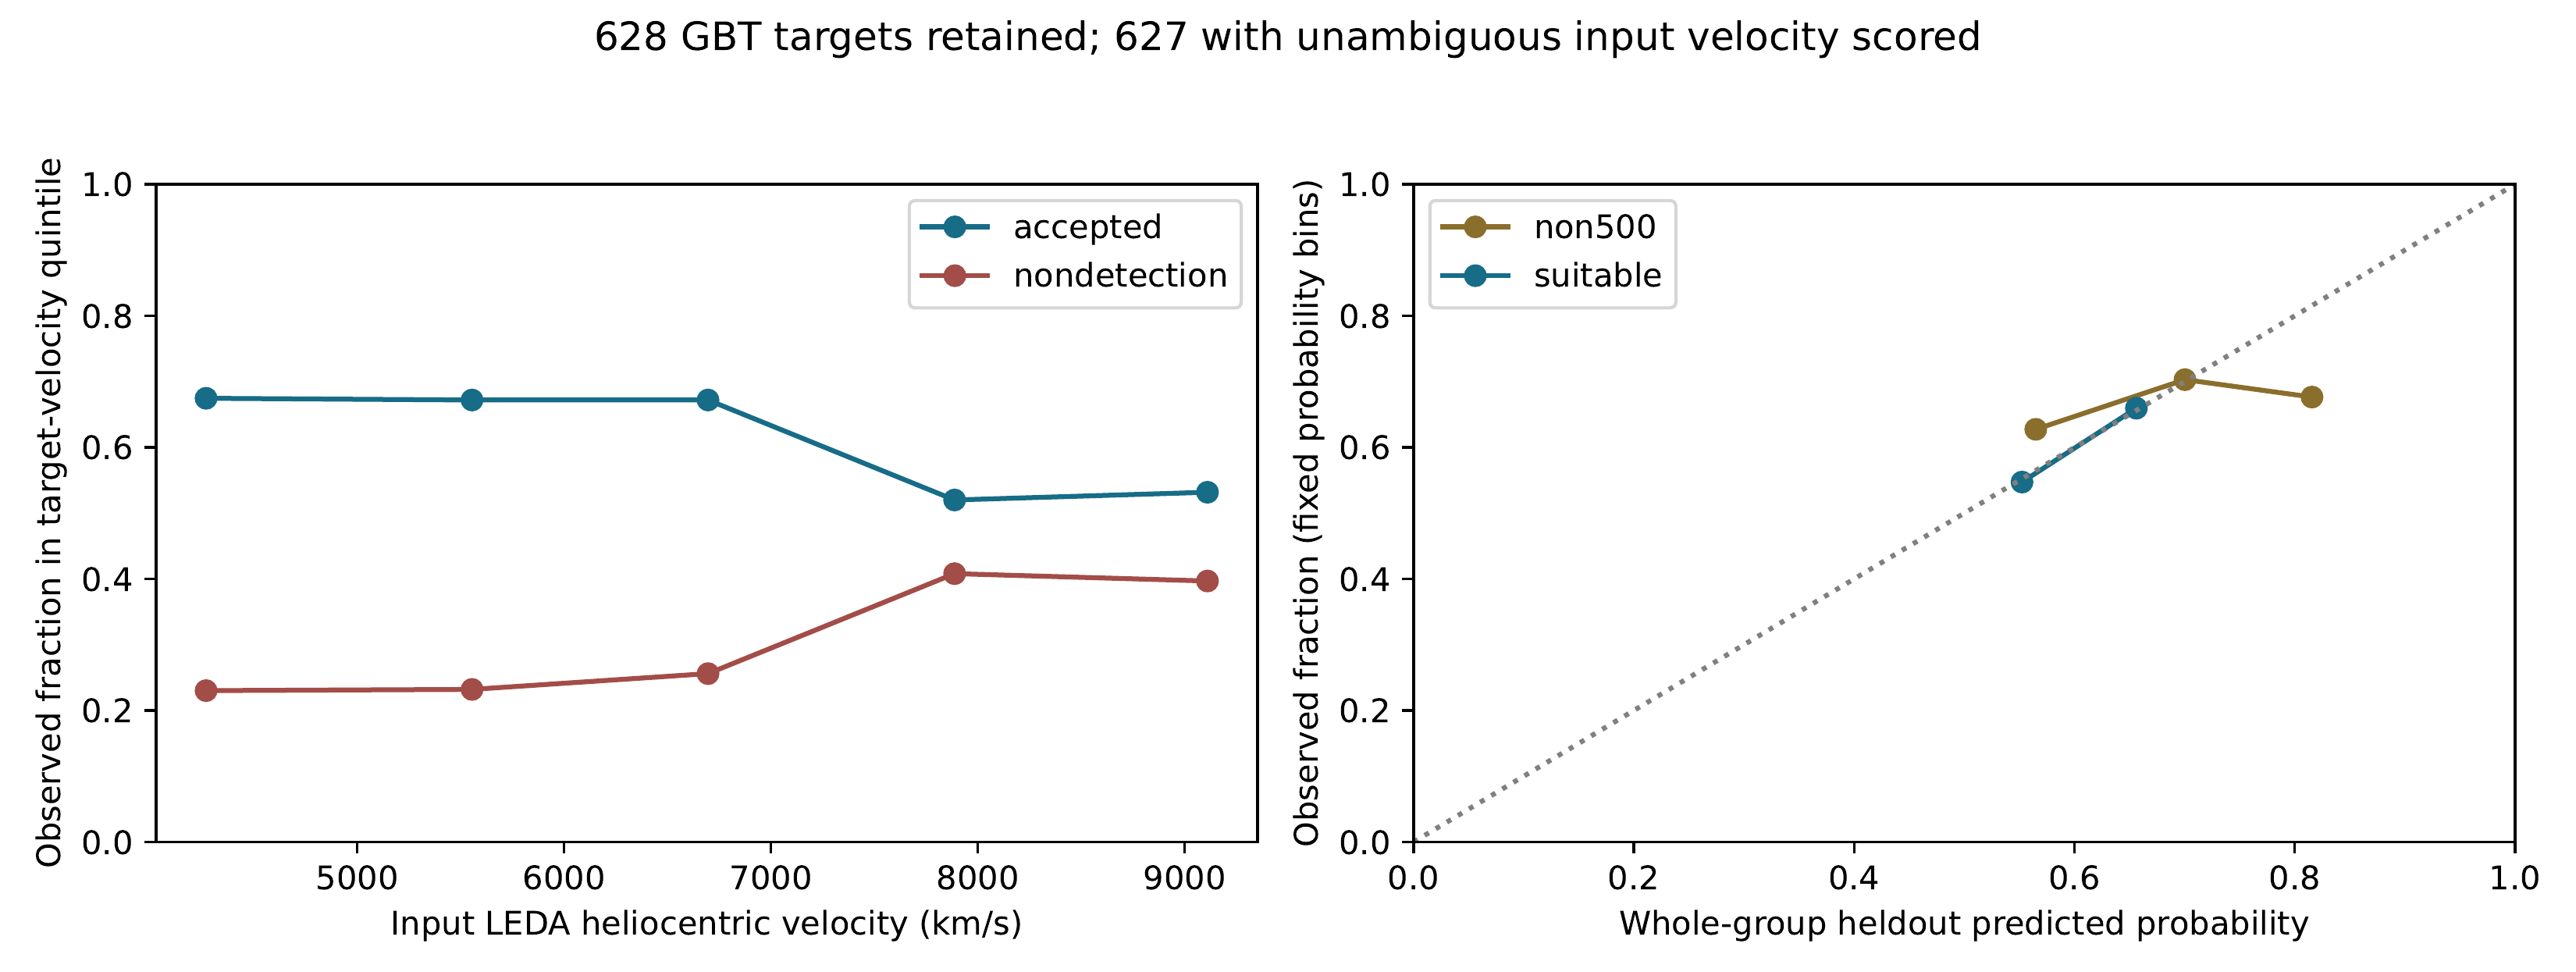
\includegraphics[width=\linewidth,height=.71\textheight,keepaspectratio]{figures/f069_external.png}
\caption{Outcome and velocity distributions in the retained hydrogen-line target cohort. Released distances, nondetections, and other quality outcomes remain distinct. These source counts and descriptive conditional fits do not supply a physical covariance or selected-parent null law.}
\label{fig:f069}
\end{figure}
\clearpage
\begin{figure}[p]
\centering
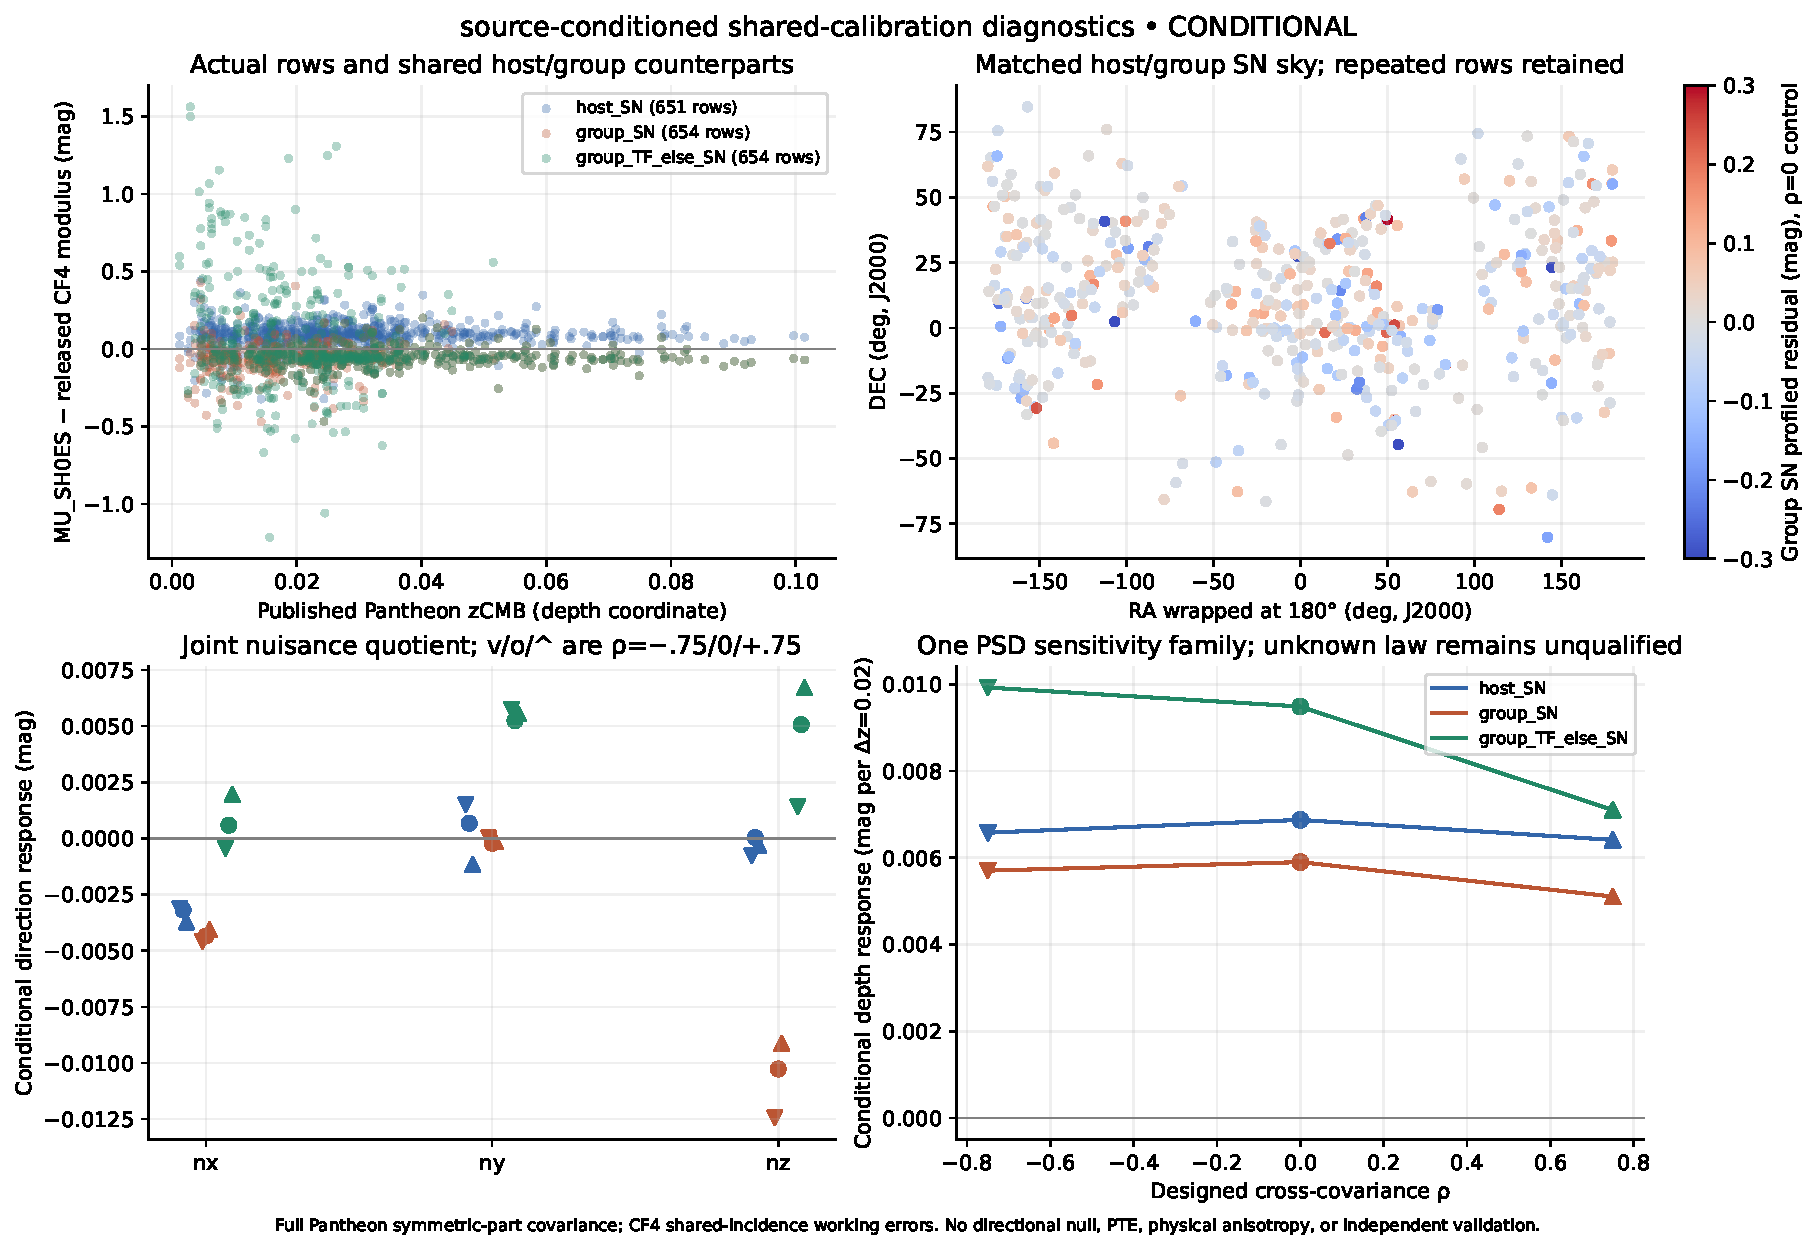
\includegraphics[width=\linewidth,height=.71\textheight,keepaspectratio]{figures/f070_external.pdf}
\caption{Pantheon+ and Cosmicflows comparisons on matched host and group sky positions. Repeated supernova rows and alternative host/group assignments are retained. Their differences are dependent source comparisons, not independent survey likelihood factors.}
\label{fig:f070}
\end{figure}
\clearpage
\begin{figure}[p]
\centering
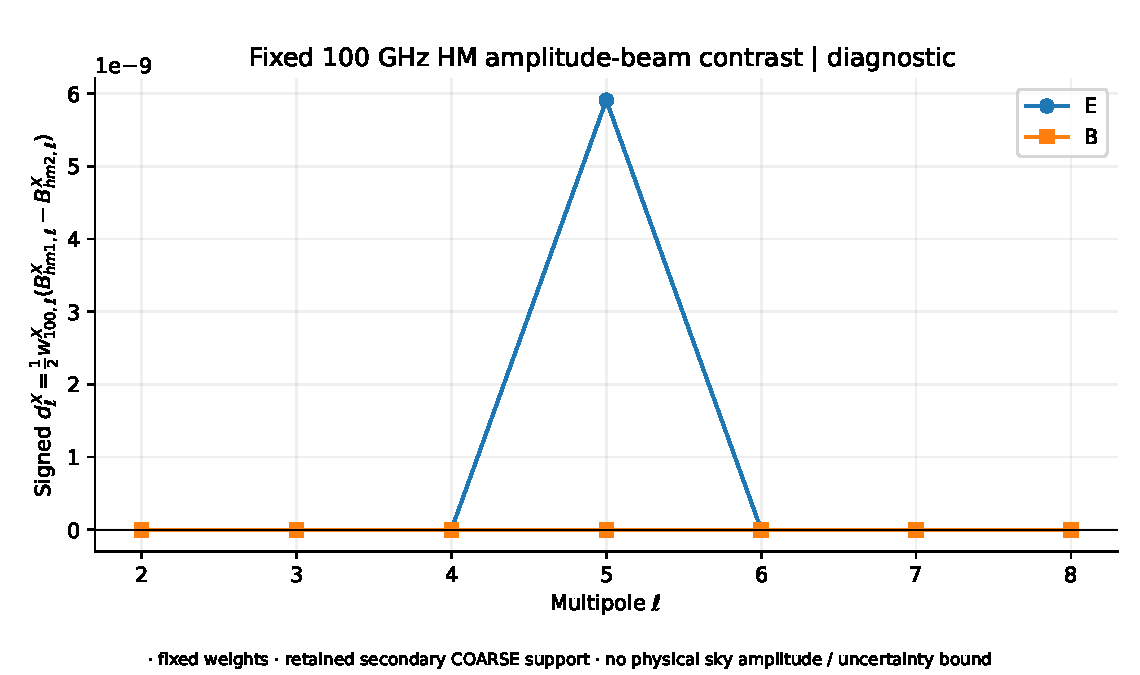
\includegraphics[width=\linewidth,height=.71\textheight,keepaspectratio]{figures/f071_external.pdf}
\caption{Fixed 100-GHz half-mission amplitude-beam contrast using retained coarse component weights. The displayed gains are properties of the declared finite operator. They are not measured sky contamination amplitudes or observational uncertainty bounds.}
\label{fig:f071}
\end{figure}
\clearpage
\begin{figure}[p]
\centering
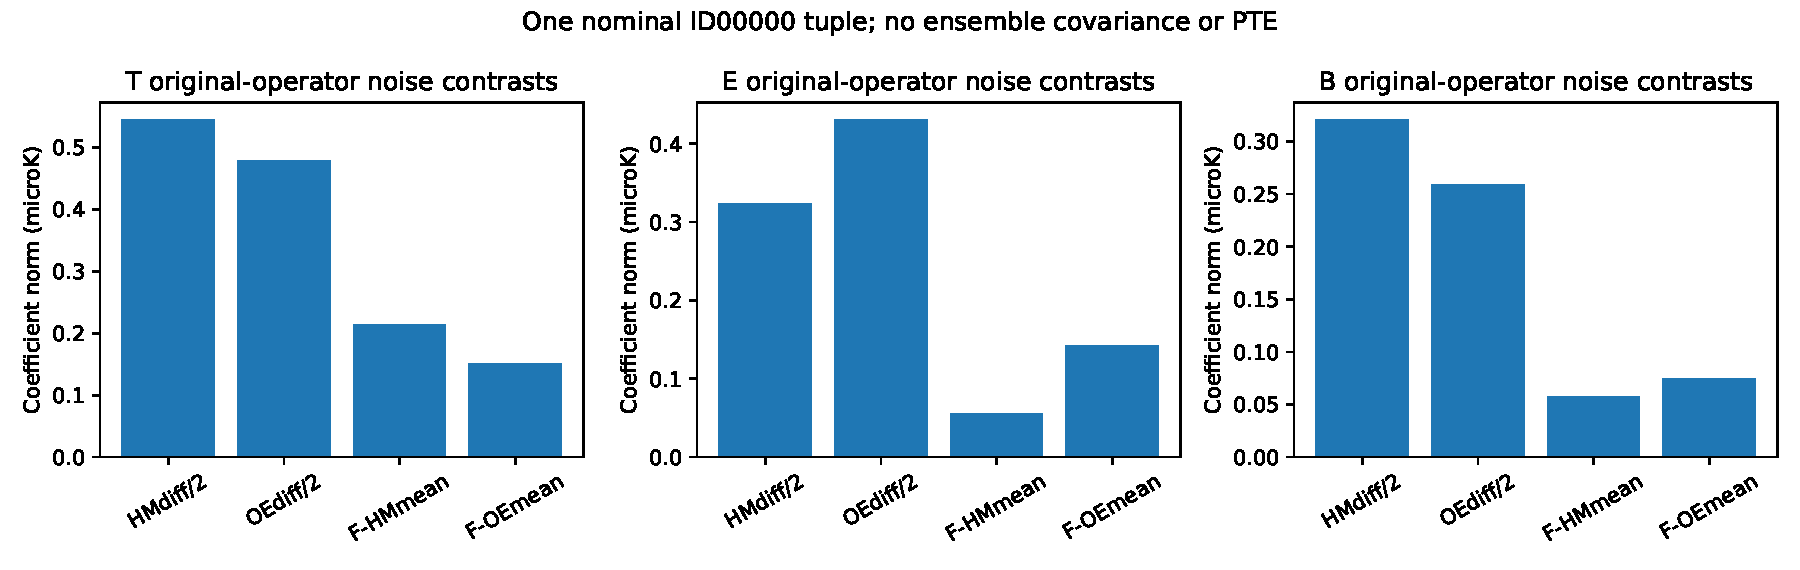
\includegraphics[width=\linewidth,height=.71\textheight,keepaspectratio]{figures/f072.pdf}
\caption{Finite split contrasts for one nominal signal/noise tuple on the stated support. A single tuple can expose a response difference but cannot estimate an ensemble covariance or a probability to exceed. Common sky components and split cross-noise remain relevant.}
\label{fig:f072}
\end{figure}
\clearpage
\begin{figure}[p]
\centering
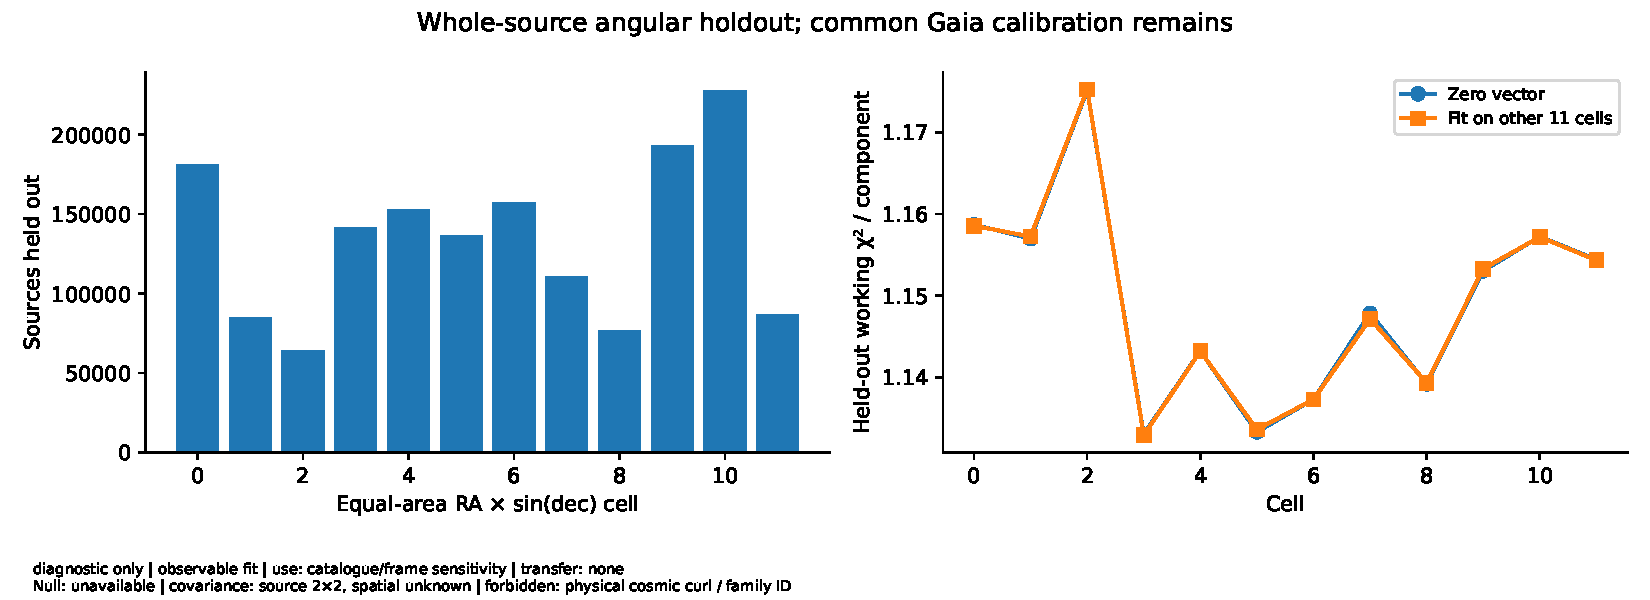
\includegraphics[width=\linewidth,height=.71\textheight,keepaspectratio]{figures/f073_external.pdf}
\caption{Whole-source angular holdout of the full Gaia frame-source sample. Held-out residual quadratics and retained counts probe spatial variation under a working covariance. Common Gaia calibration survives this split, so it does not create an independent physical validation sample.}
\label{fig:f073}
\end{figure}
\clearpage
\begin{figure}[p]
\centering
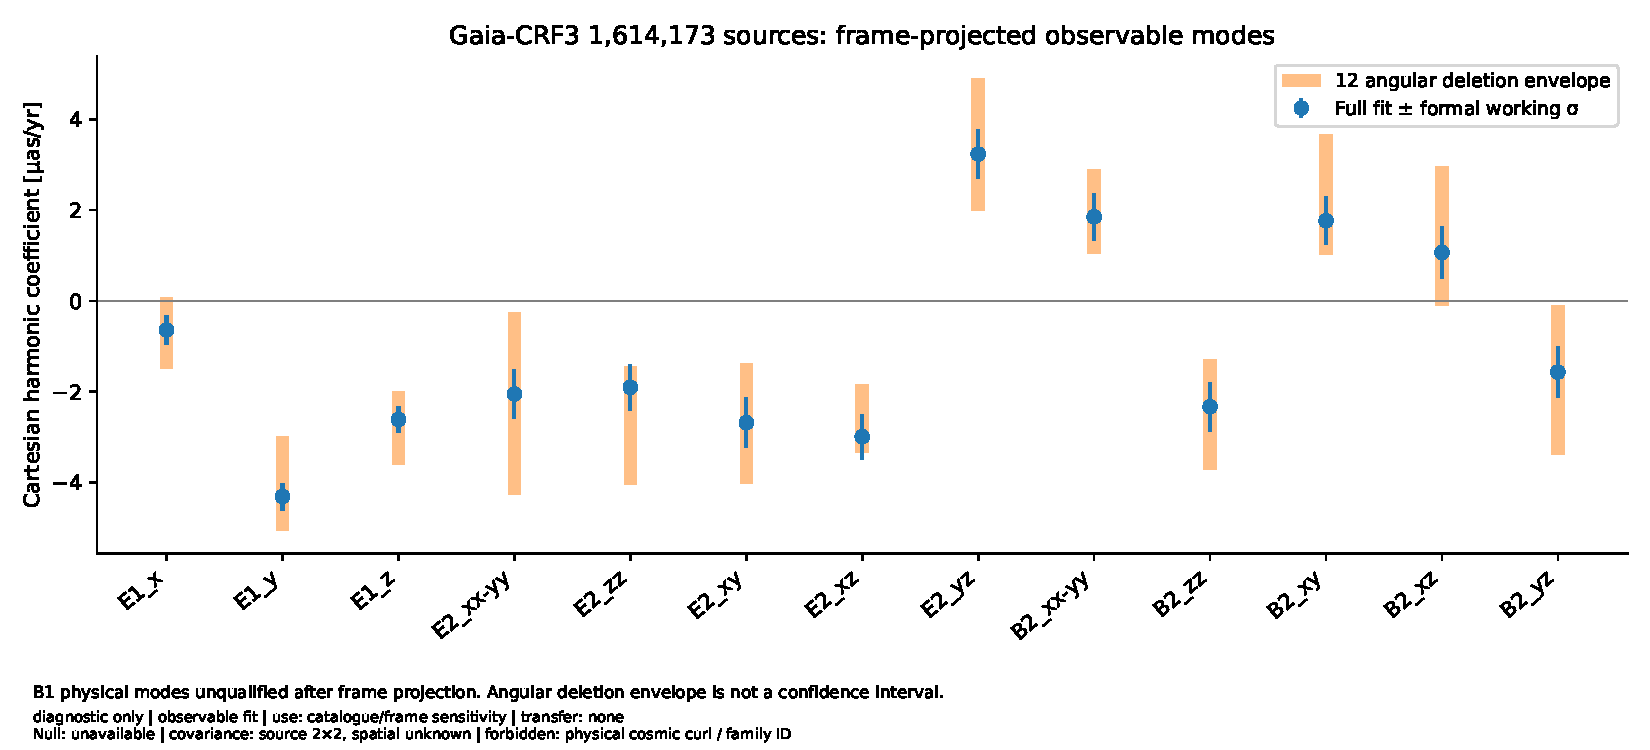
\includegraphics[width=\linewidth,height=.71\textheight,keepaspectratio]{figures/f074_external.pdf}
\caption{Frame-projected vector-spherical-harmonic coefficients in the full Gaia-CRF3 catalogue, with angular-deletion sensitivity. Formal errors use reported source blocks. The retained vector and STF modes are observable fields, not directly measured matter acceleration, shear, or vorticity.}
\label{fig:f074}
\end{figure}
\clearpage
\begin{figure}[p]
\centering
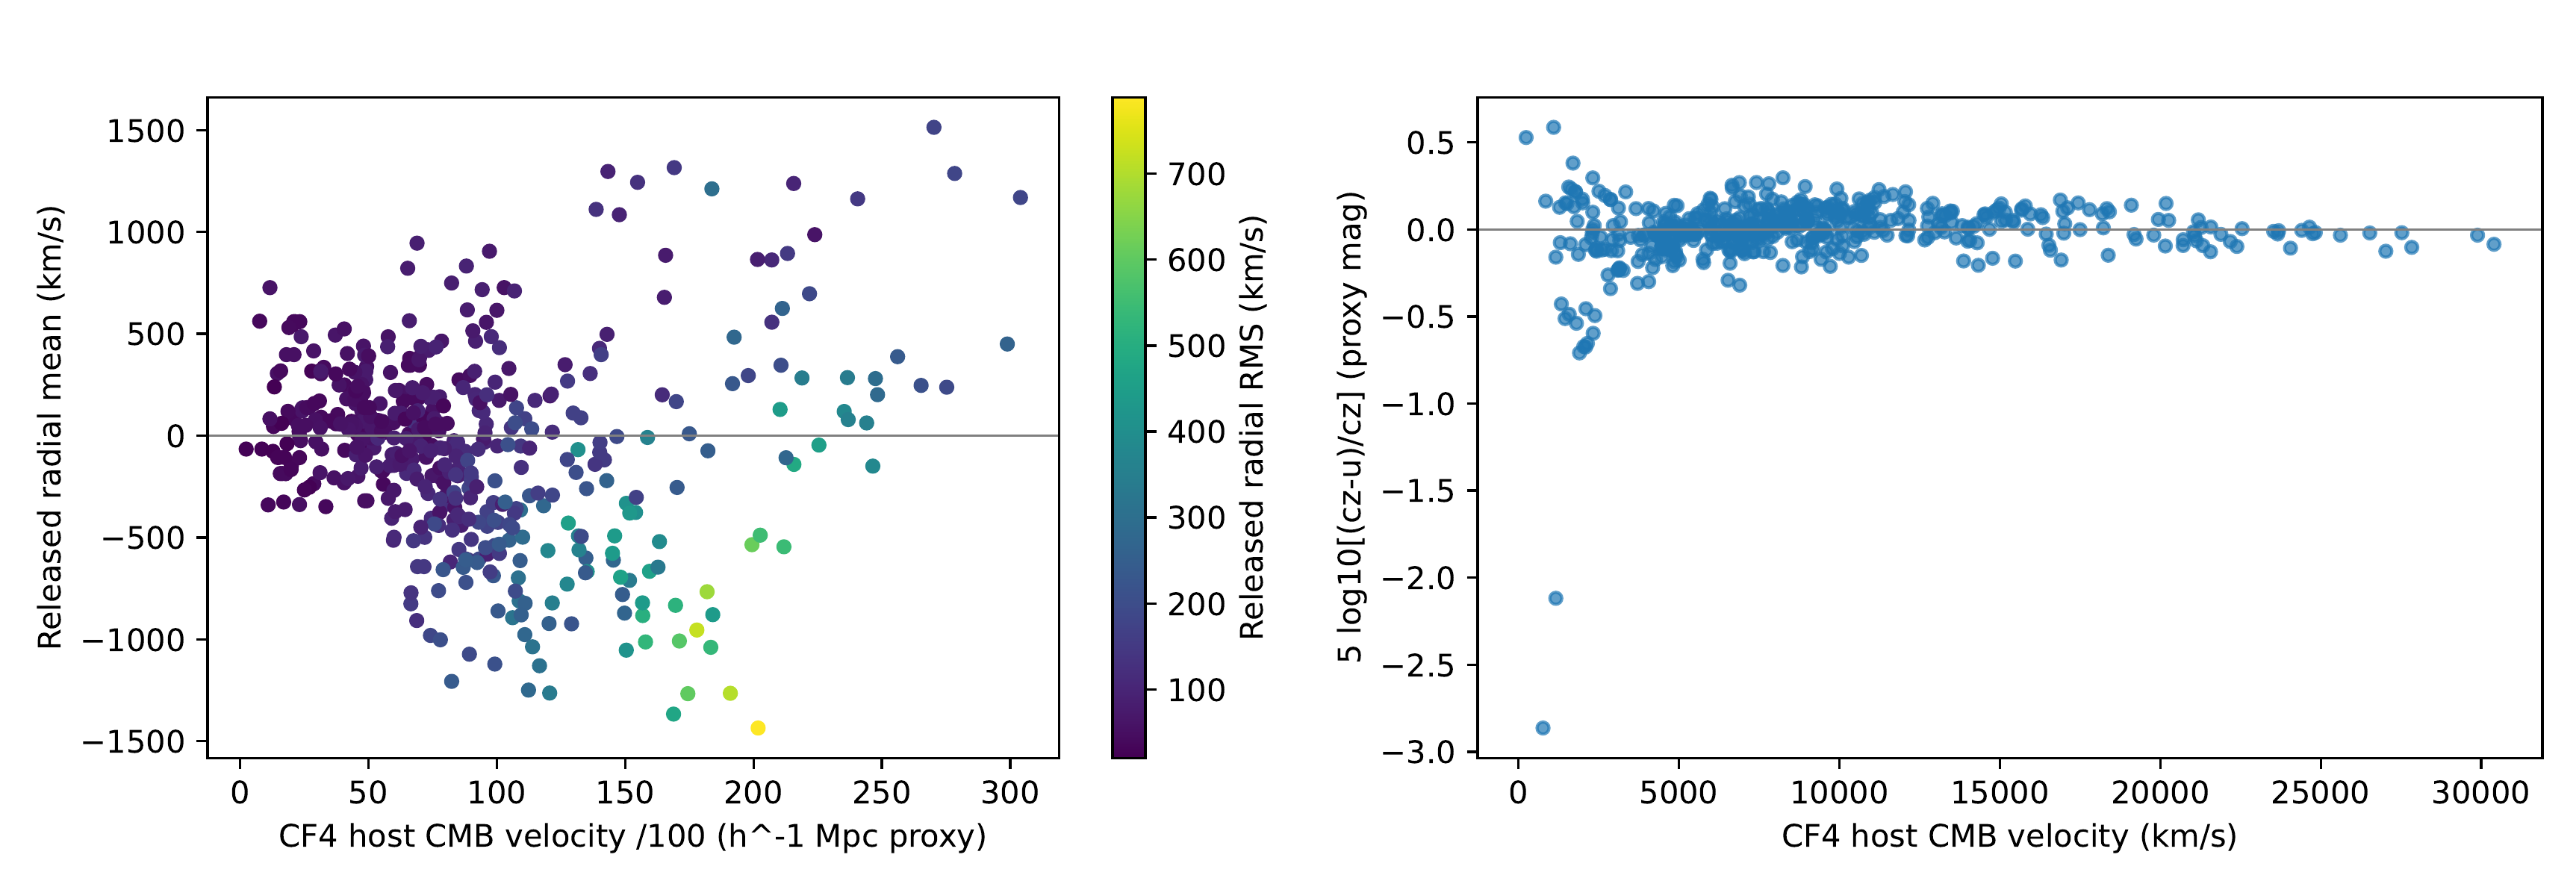
\includegraphics[width=\linewidth,height=.71\textheight,keepaspectratio]{figures/f075_external.png}
\caption{Corrected Cosmicflows reconstruction evaluated at matched hosts. Radial values and magnitude shifts are dependent source and algebraic proxy diagnostics. The lookup is not a physical luminosity-distance correction and has no supplied joint covariance with the host distances.}
\label{fig:f075}
\end{figure}
\clearpage
\begin{figure}[p]
\centering
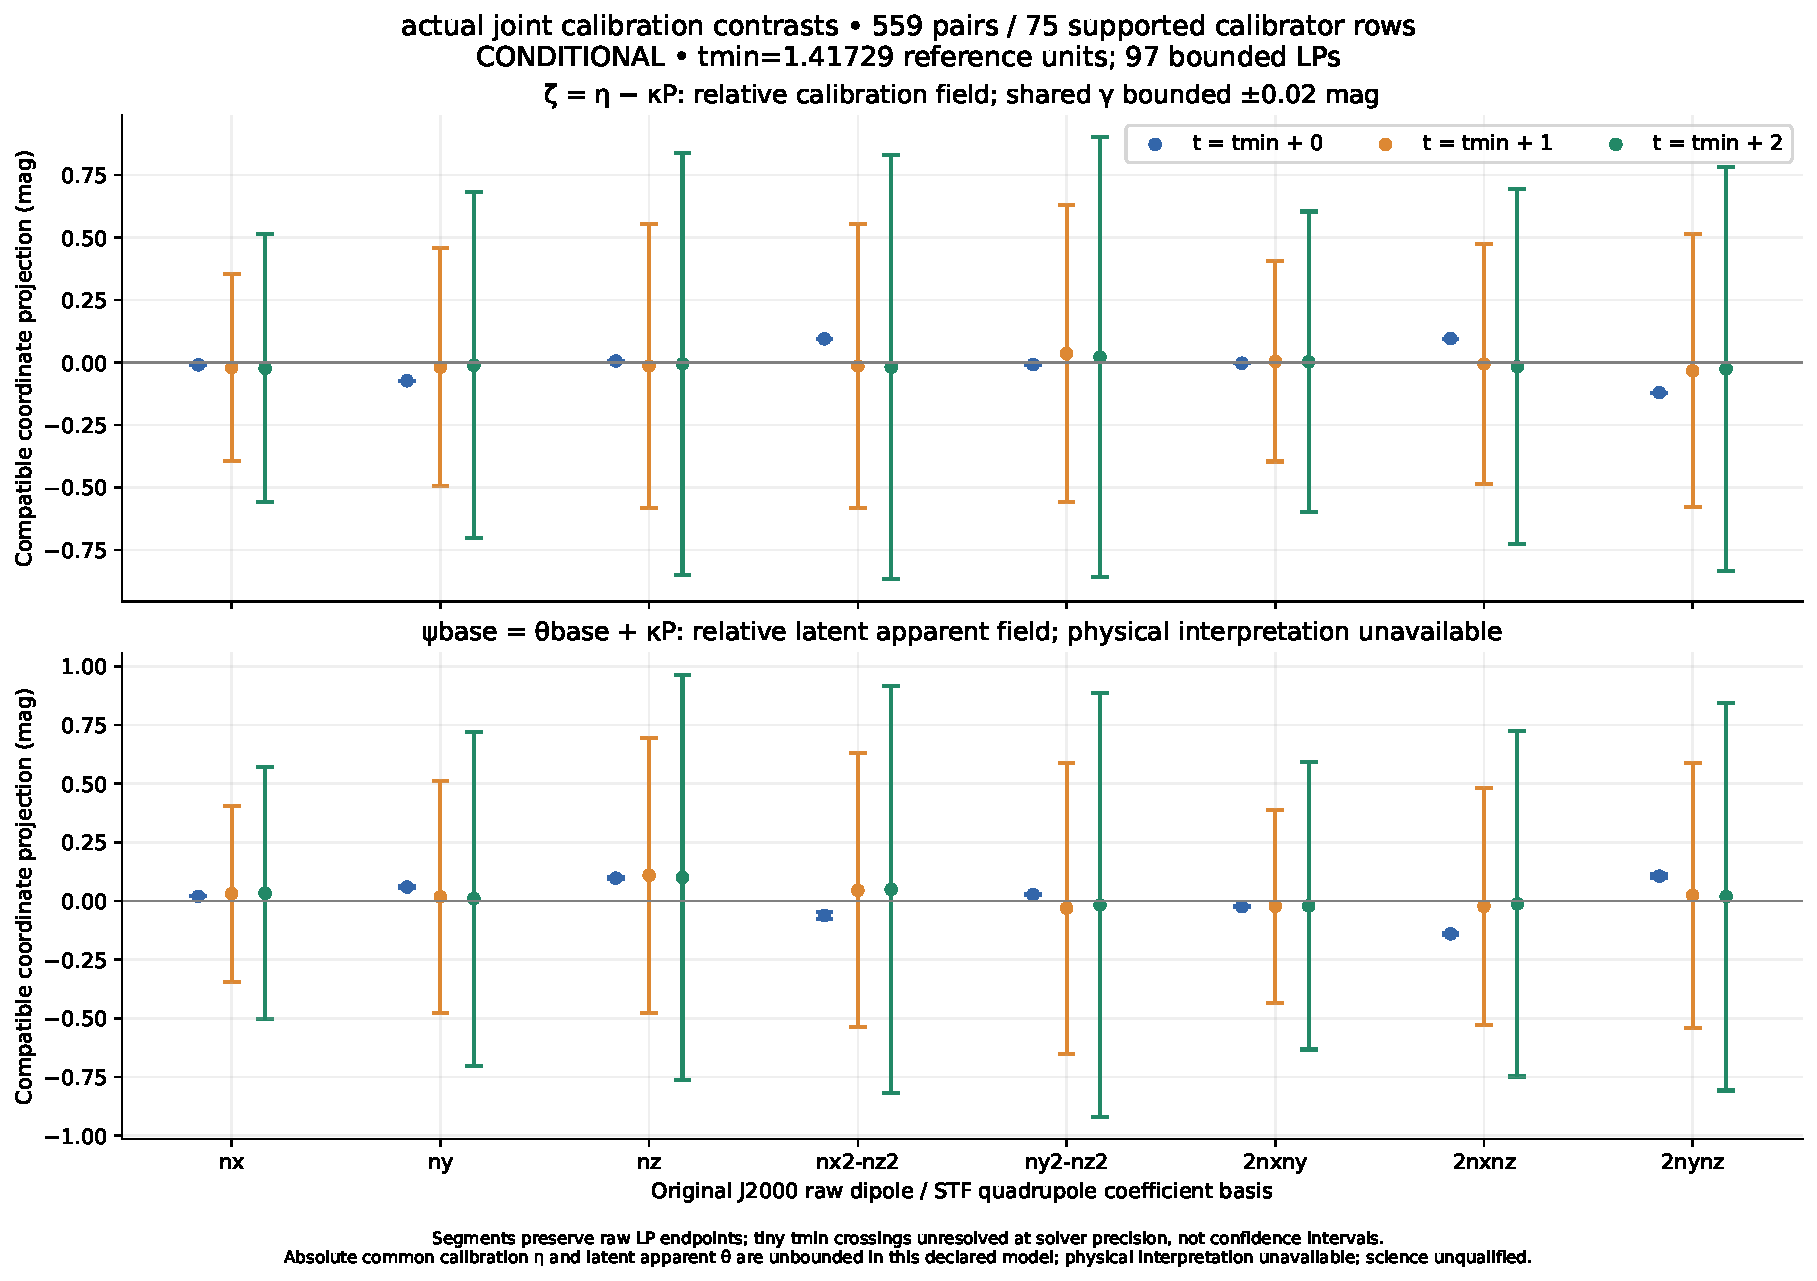
\includegraphics[width=\linewidth,height=.71\textheight,keepaspectratio]{figures/f076_external.pdf}
\caption{Joint calibration contrasts on shared hosts and groups. Identified combinations have bounded reference-coordinate projections, while common absolute calibration and other gauge directions remain unbounded. The minimum reference radius is dimensionless and is not a noise quantile or physical confidence bound.}
\label{fig:f076}
\end{figure}
\clearpage
\begin{figure}[p]
\centering
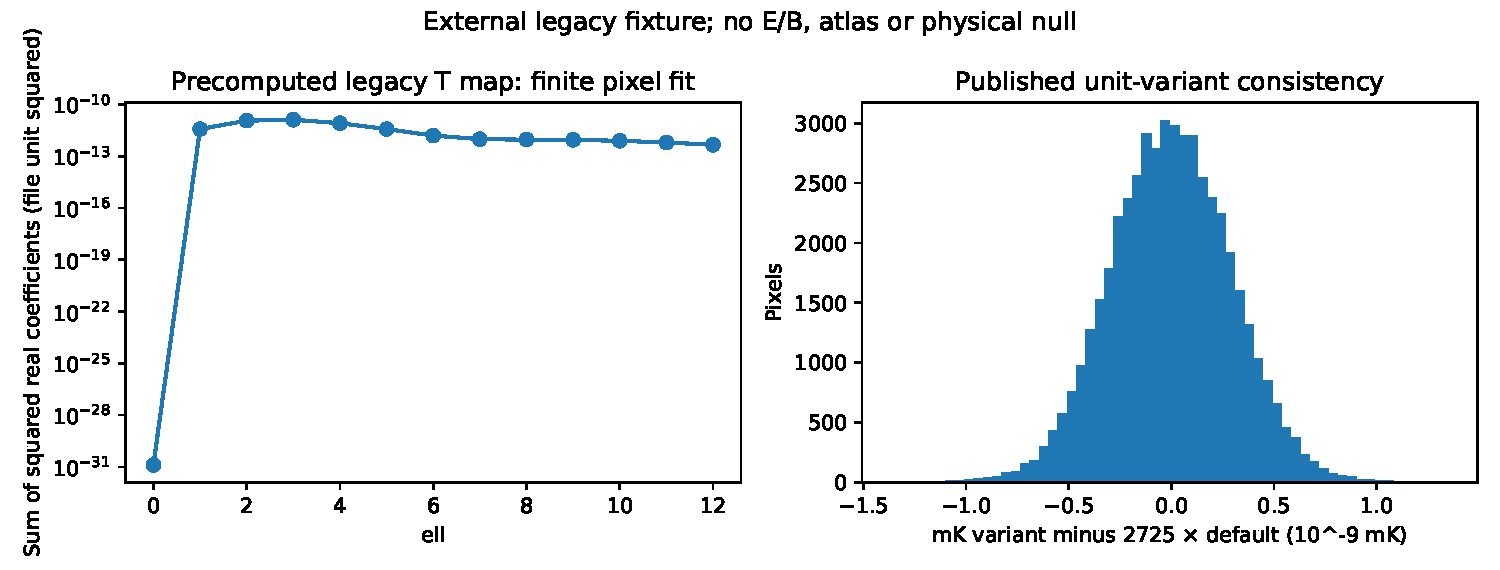
\includegraphics[width=\linewidth,height=.71\textheight,keepaspectratio]{figures/f077.pdf}
\caption{Finite harmonic representation of a precomputed external temperature-only template and its unit variants. Polarization is absent, not zero; the absolute sky frame and physical atlas eligibility are unqualified. This external template is not a native solver result.}
\label{fig:f077}
\end{figure}
\clearpage
\begin{figure}[p]
\centering
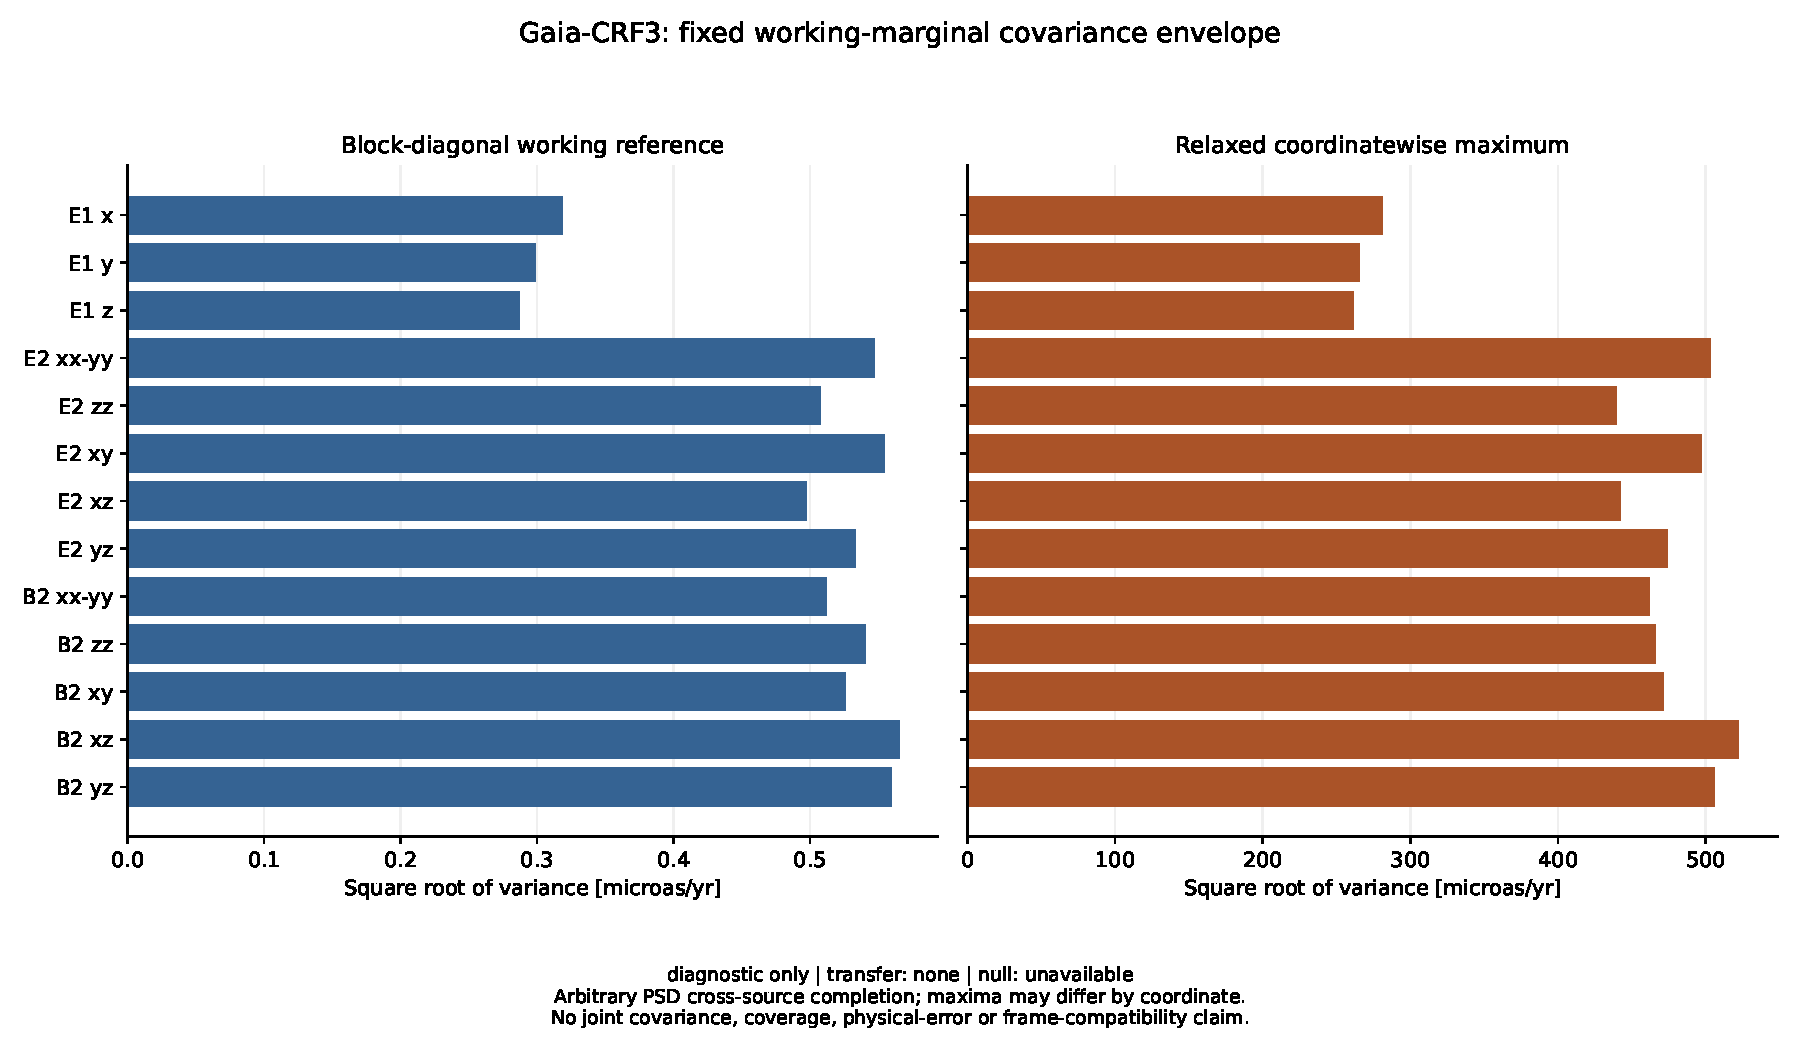
\includegraphics[width=\linewidth,height=.71\textheight,keepaspectratio]{figures/f078_external.pdf}
\caption{Coordinatewise covariance envelopes for the Gaia observable fit with working marginals held fixed. Arbitrary positive-semidefinite dependence can enlarge individual error scales. Different extrema are not jointly attainable by assumption, and the plot is not a measured spatial covariance or one matrix upper bound.}
\label{fig:f078}
\end{figure}
\clearpage
\begin{figure}[p]
\centering
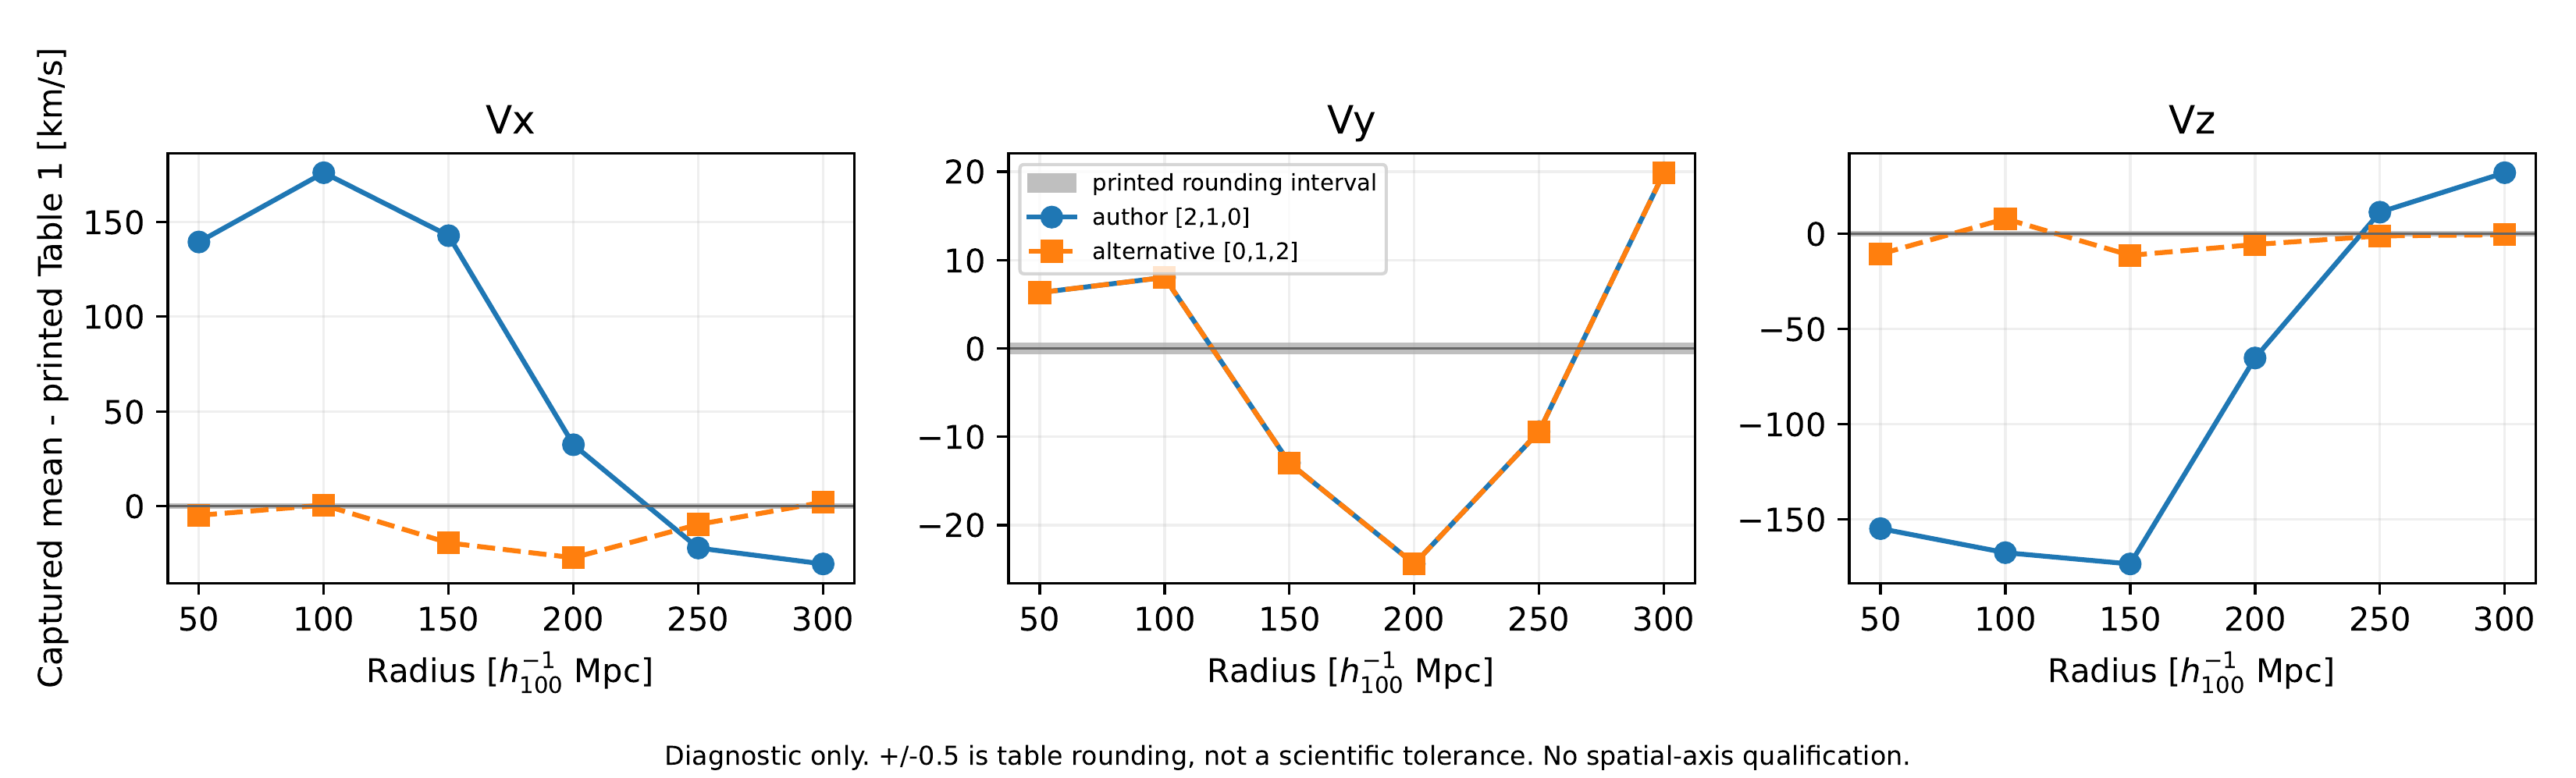
\includegraphics[width=\linewidth,height=.71\textheight,keepaspectratio]{figures/f079_external.png}
\caption{Comparison of a captured grouped-flow source with its printed summary under the specified coordinate-order alternatives. The source discrepancy remains unresolved. Neither coordinate substitution nor a close subset comparison establishes full source parity.}
\label{fig:f079}
\end{figure}
\clearpage
\begin{figure}[p]
\centering
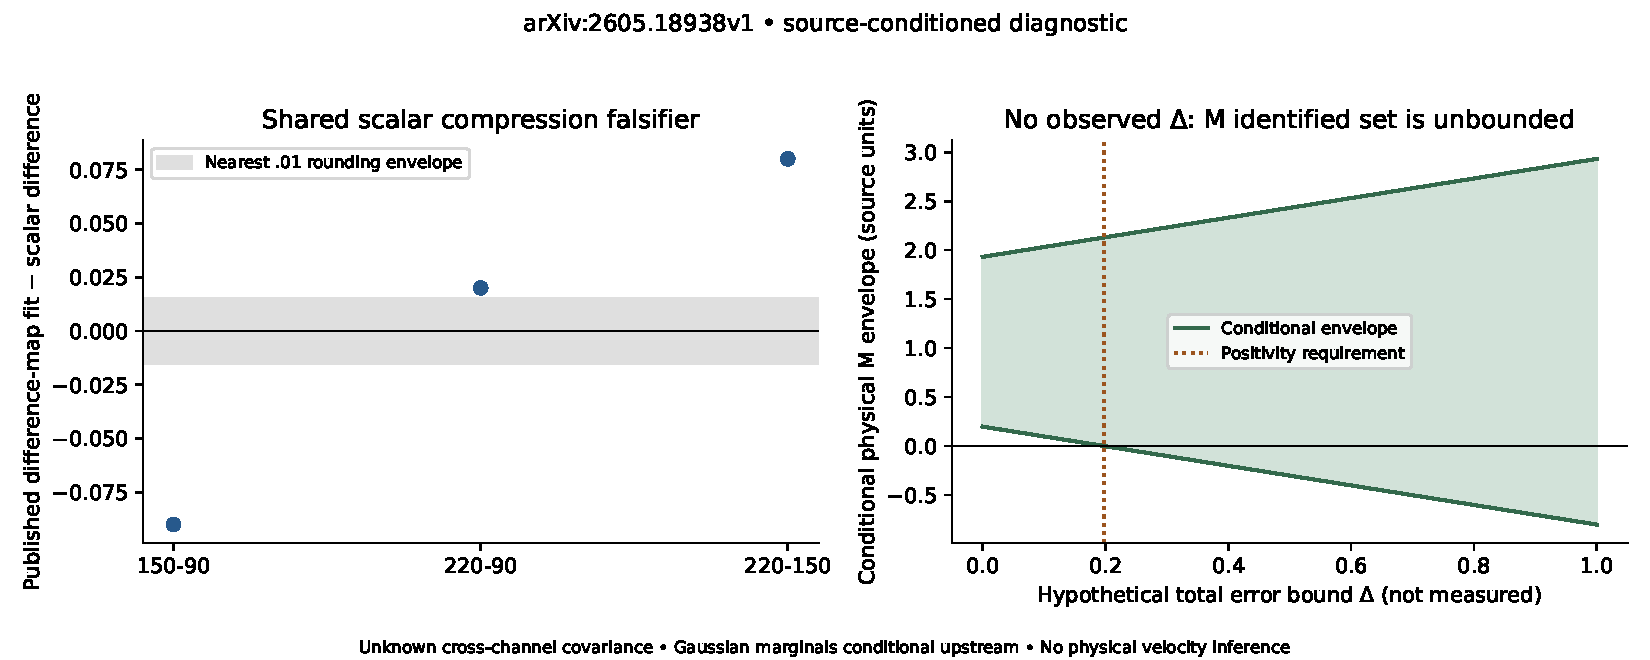
\includegraphics[width=\linewidth,height=.71\textheight,keepaspectratio]{figures/f080_external.pdf}
\caption{Source-conditioned moving-lens amplitude contrasts and a falsifier of shared scalar compression. The displayed intervals assume the stated marginal laws and rounding allowance. No observed differential filter or spectral-error bound is supplied; the physical amplitude therefore remains unbounded.}
\label{fig:f080}
\end{figure}
\clearpage
\begin{figure}[p]
\centering
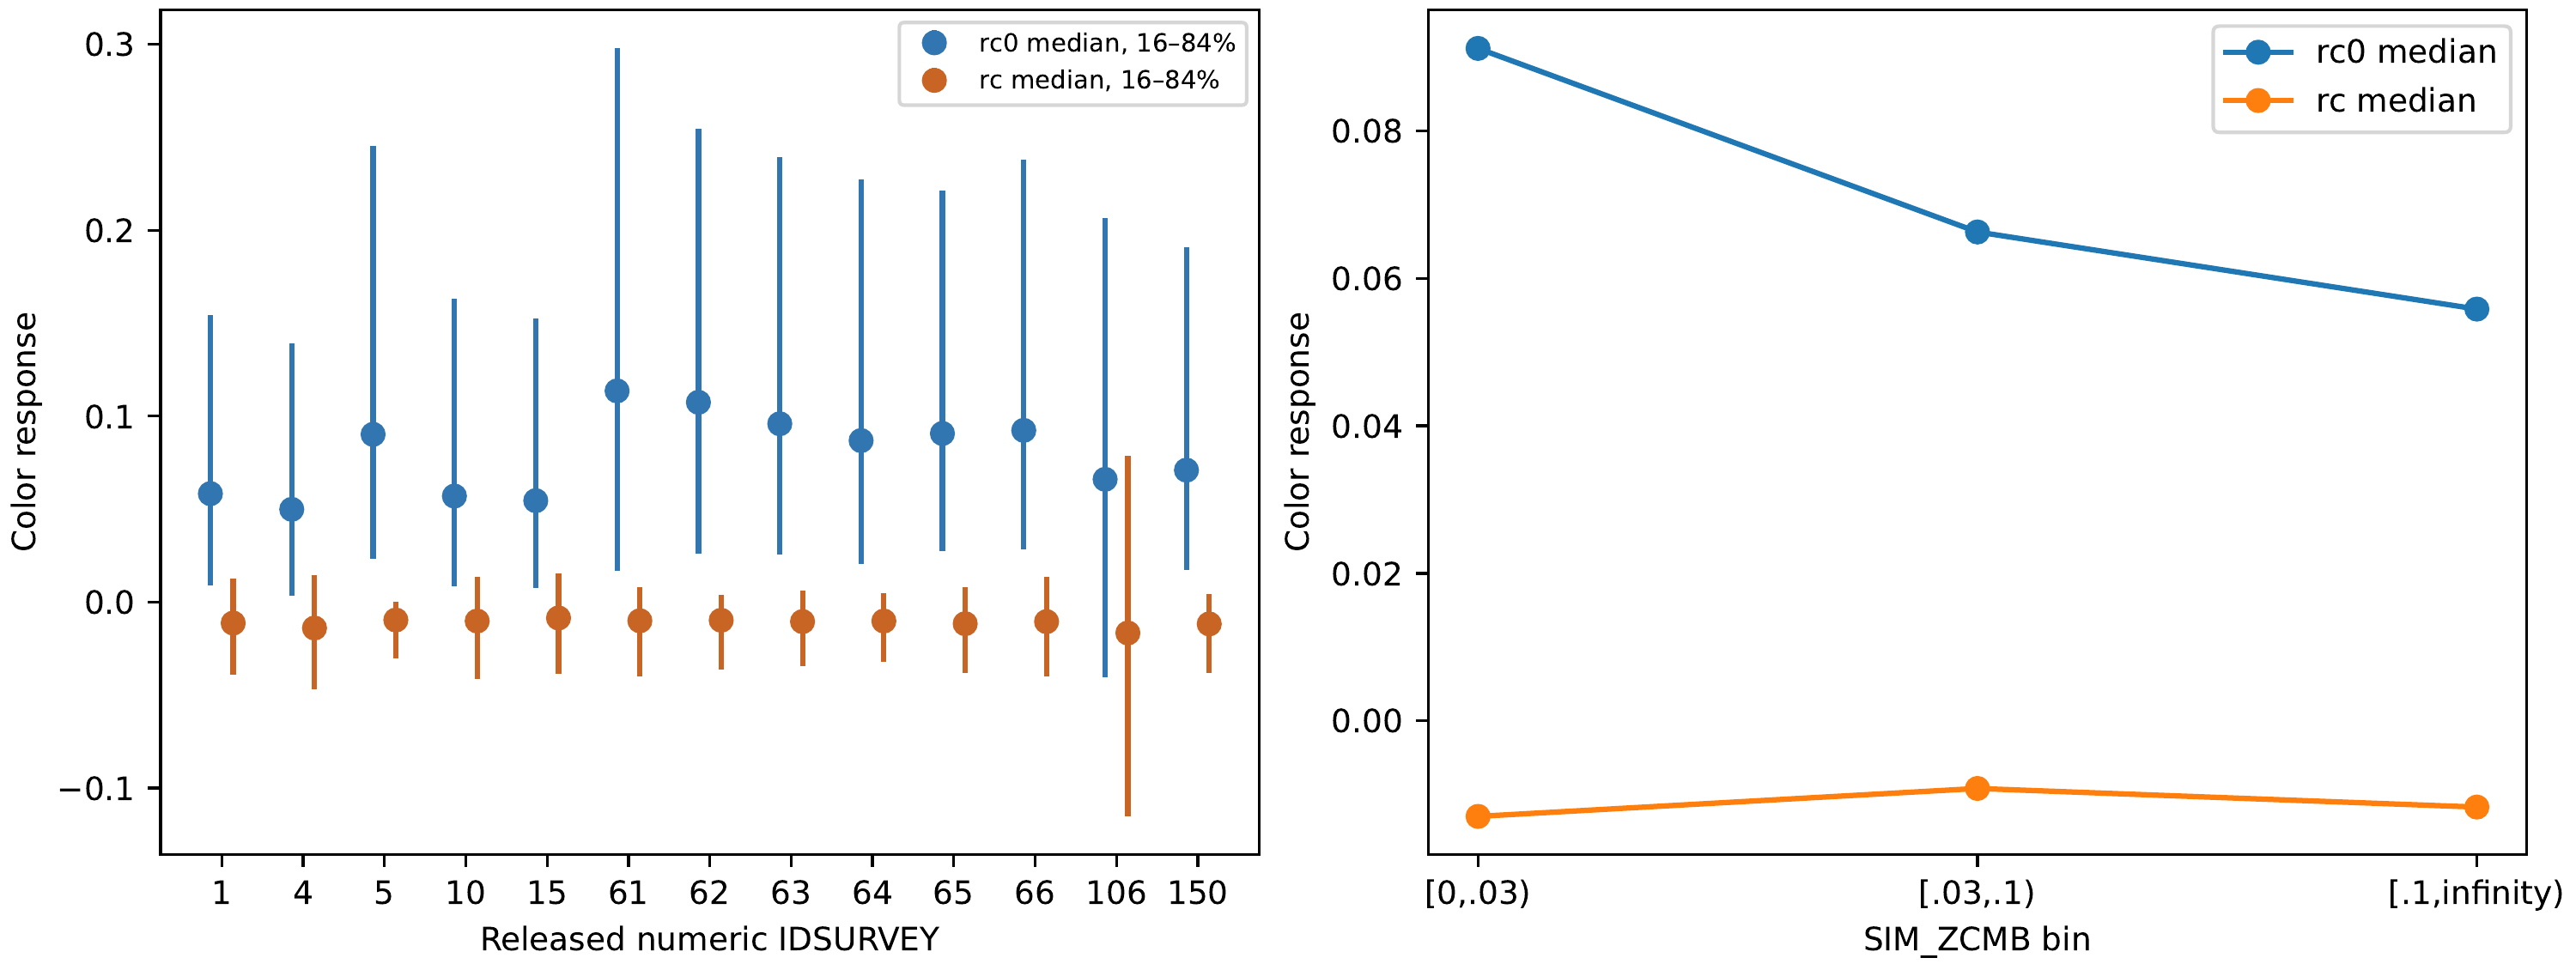
\includegraphics[width=\linewidth,height=.71\textheight,keepaspectratio]{figures/f081_external.png}
\caption{Colour response in released selected supernova simulations, before and after the stated dust-predictor adjustment. The rows and source model define this simulation diagnostic. It is not an empirical total reboost response or calibrated observed-survey correction.}
\label{fig:f081}
\end{figure}
\clearpage
\begin{figure}[p]
\centering
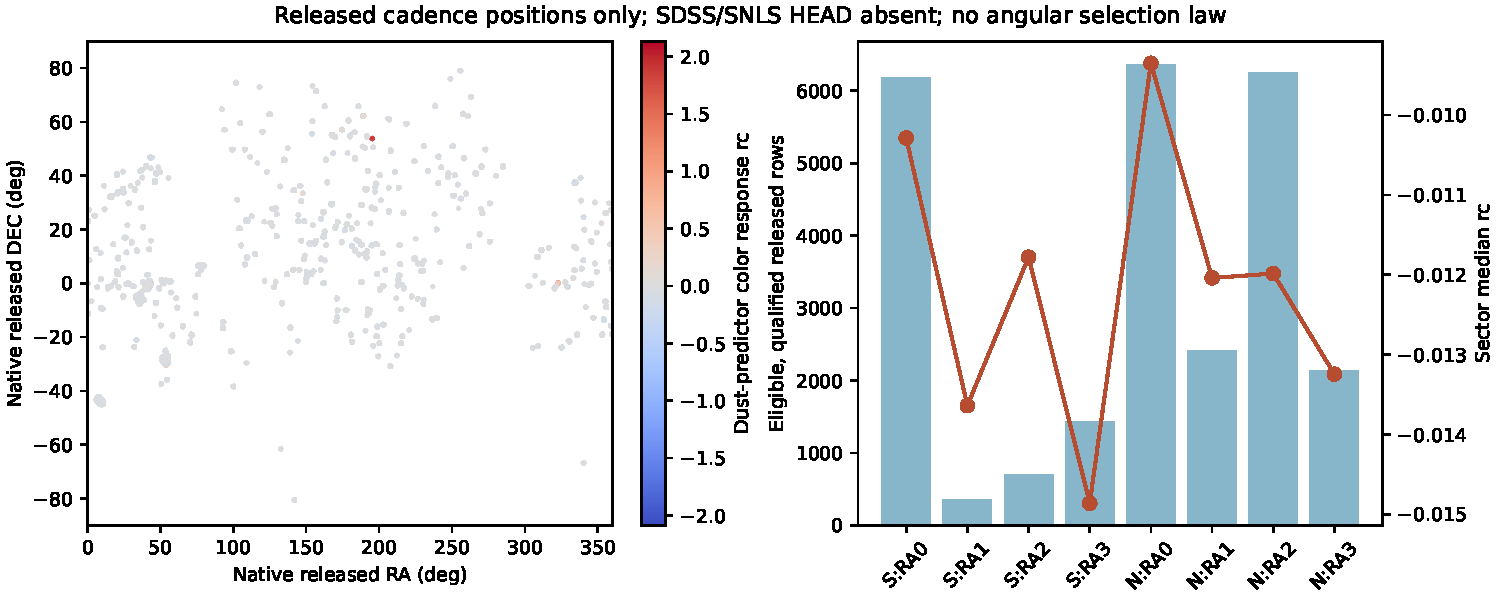
\includegraphics[width=\linewidth,height=.71\textheight,keepaspectratio]{figures/f082.pdf}
\caption{Released directions and sky variation of the selected supernova simulation response. Qualified angular coordinates are retained, with missing directions excluded explicitly. Directional patterns in these simulations do not establish physical sky anisotropy.}
\label{fig:f082}
\end{figure}
\clearpage
\begin{figure}[p]
\centering
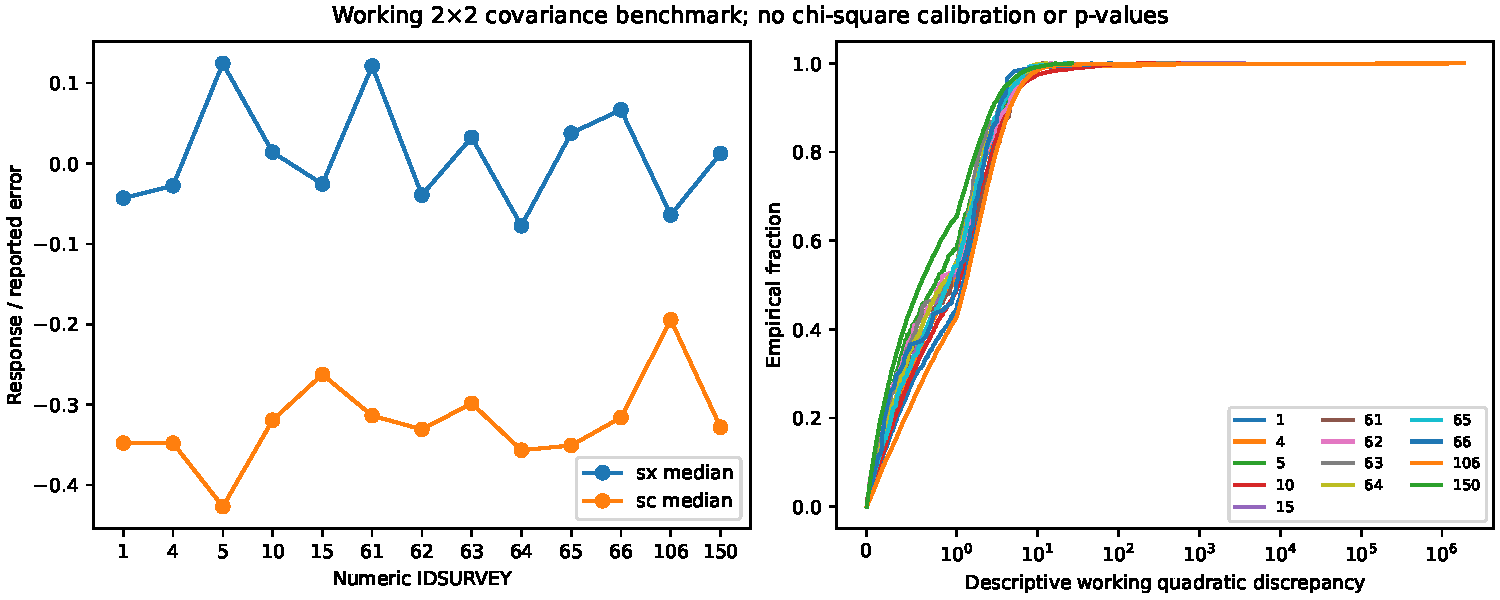
\includegraphics[width=\linewidth,height=.71\textheight,keepaspectratio]{figures/f083.pdf}
\caption{Working two-coordinate covariance benchmark for released supernova simulation responses. The displayed standardized responses and empirical fractions use their source-specific errors. No chi-square calibration, physical probability, or new observed-supernova likelihood is assigned.}
\label{fig:f083}
\end{figure}
\clearpage
\begin{figure}[p]
\centering
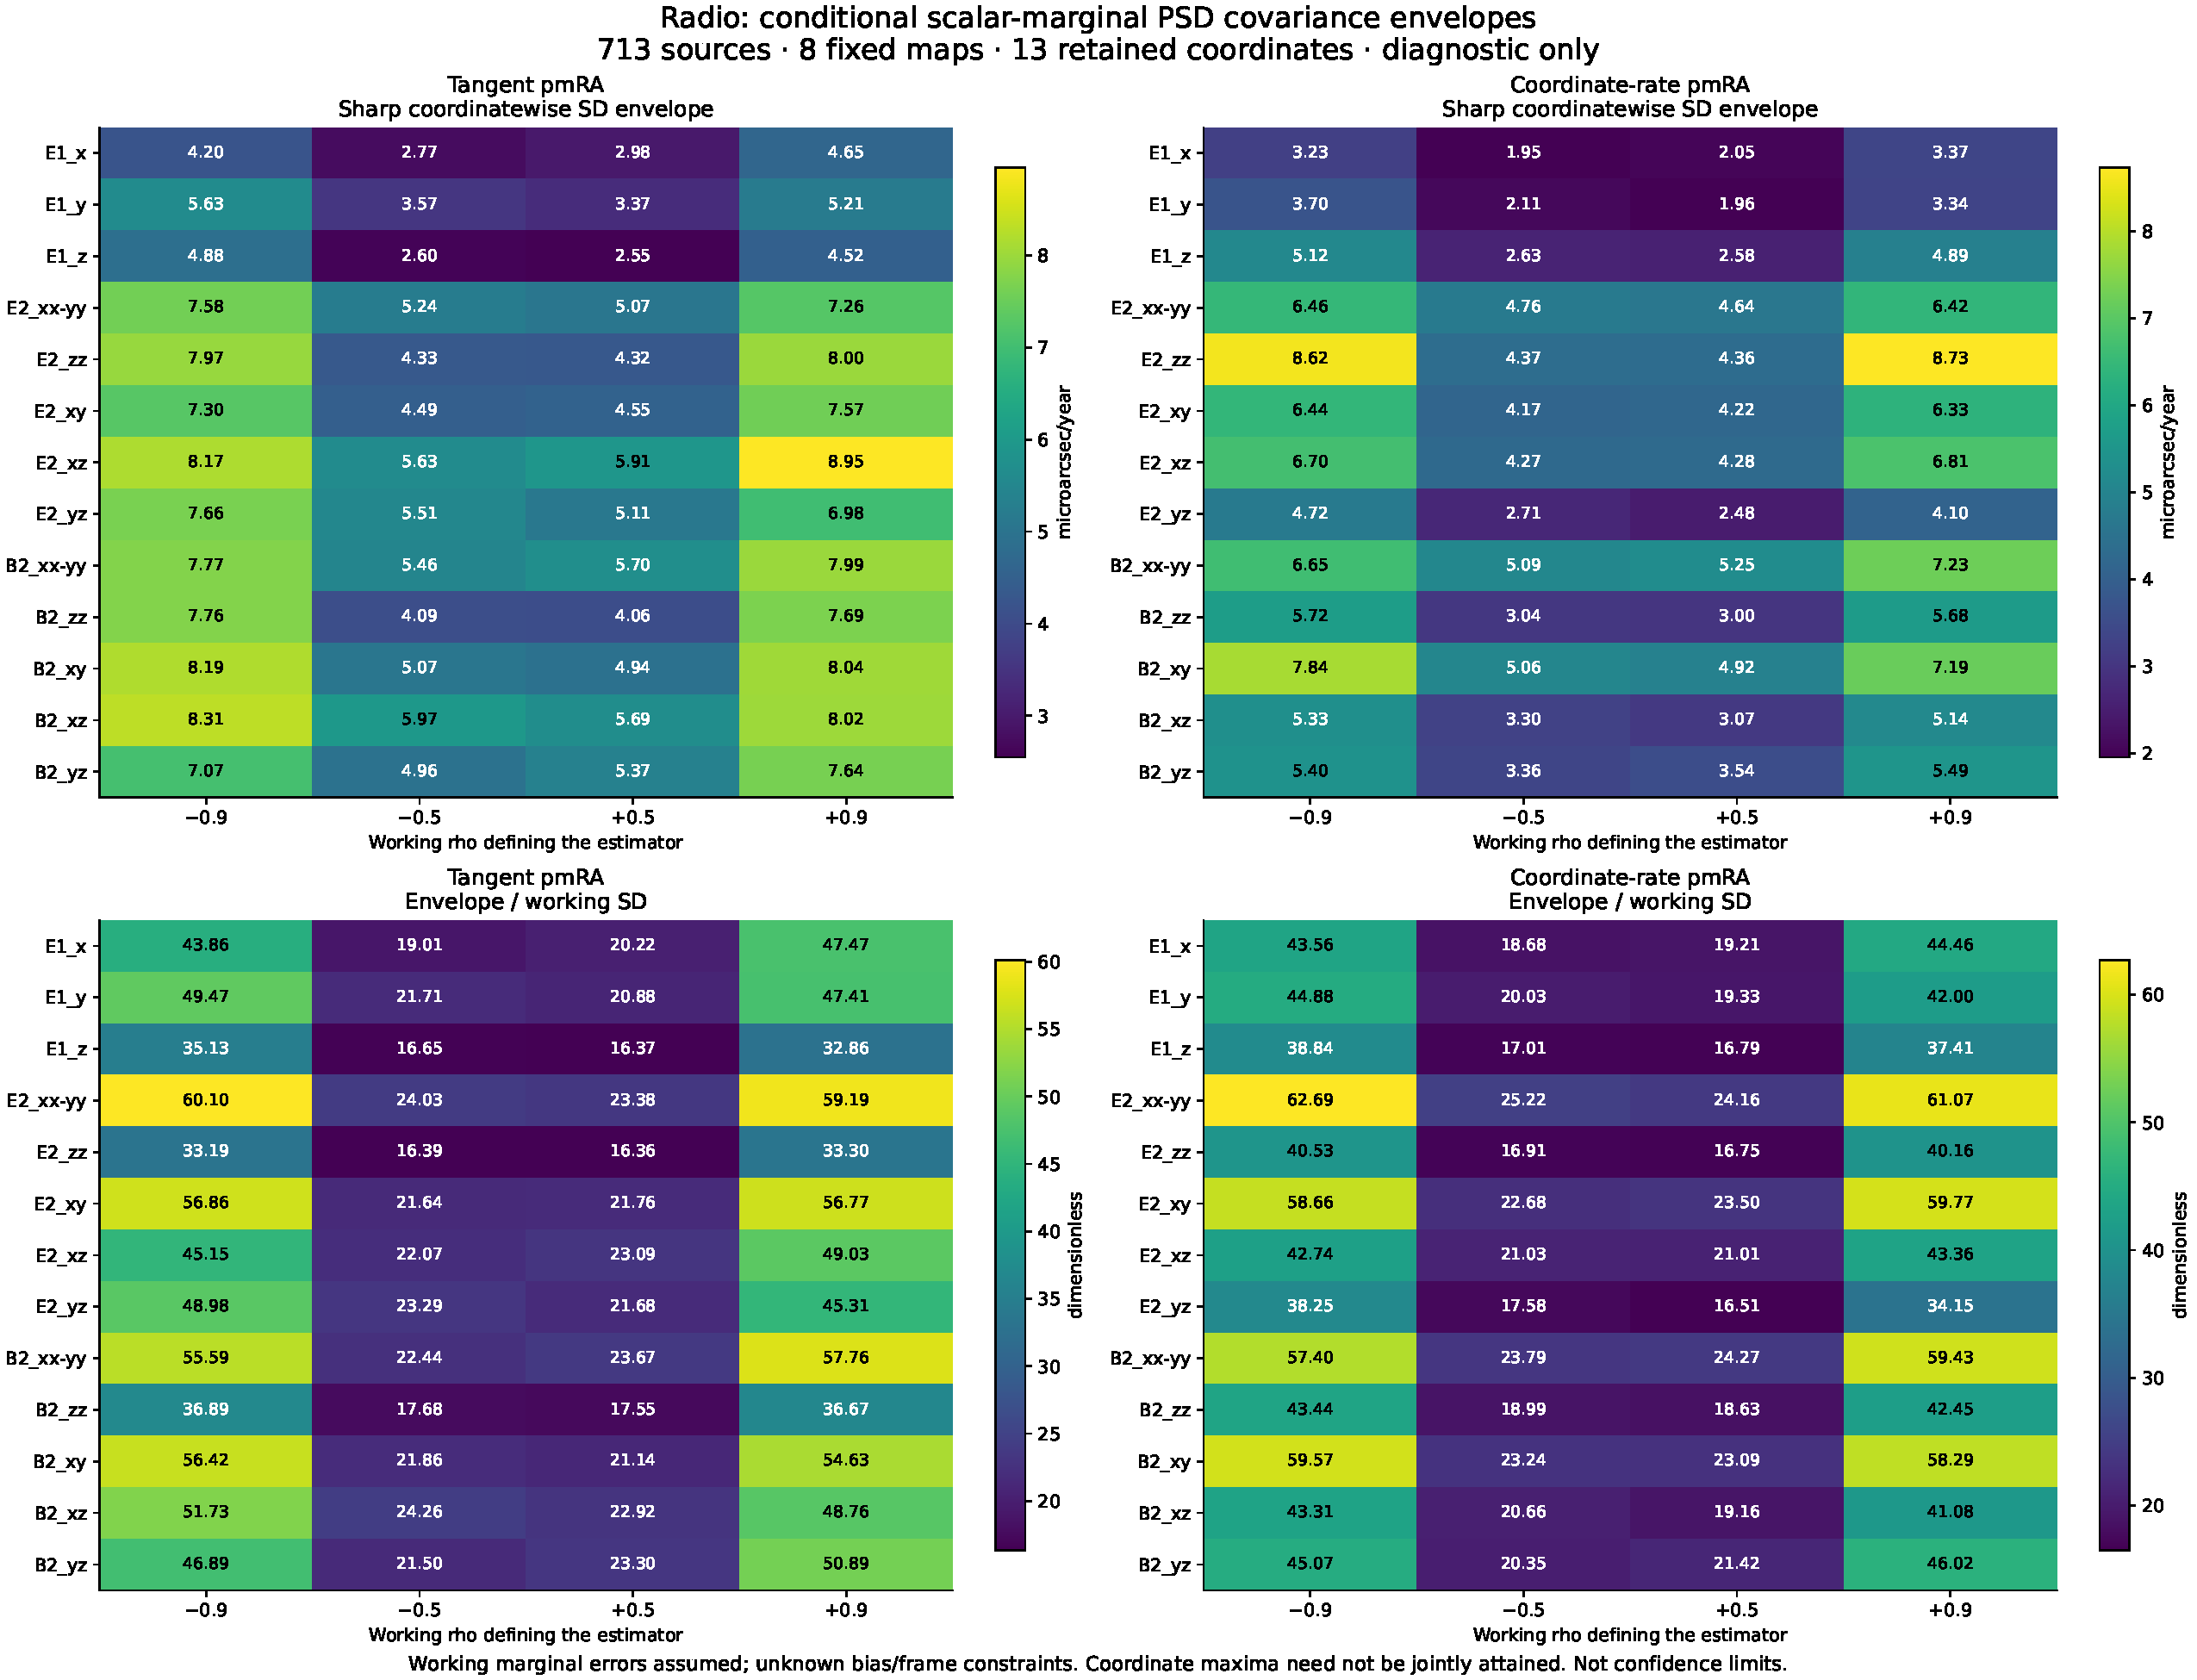
\includegraphics[width=\linewidth,height=.71\textheight,keepaspectratio]{figures/f084_external.pdf}
\caption{Radio proper-motion coordinate envelopes under fixed scalar marginals and stated correlation scenarios. The retained coordinate convention matters. These are separate sharp coordinate bounds, not a jointly attained covariance matrix or a calibrated optical--radio physical comparison.}
\label{fig:f084}
\end{figure}
\clearpage
\begin{figure}[p]
\centering
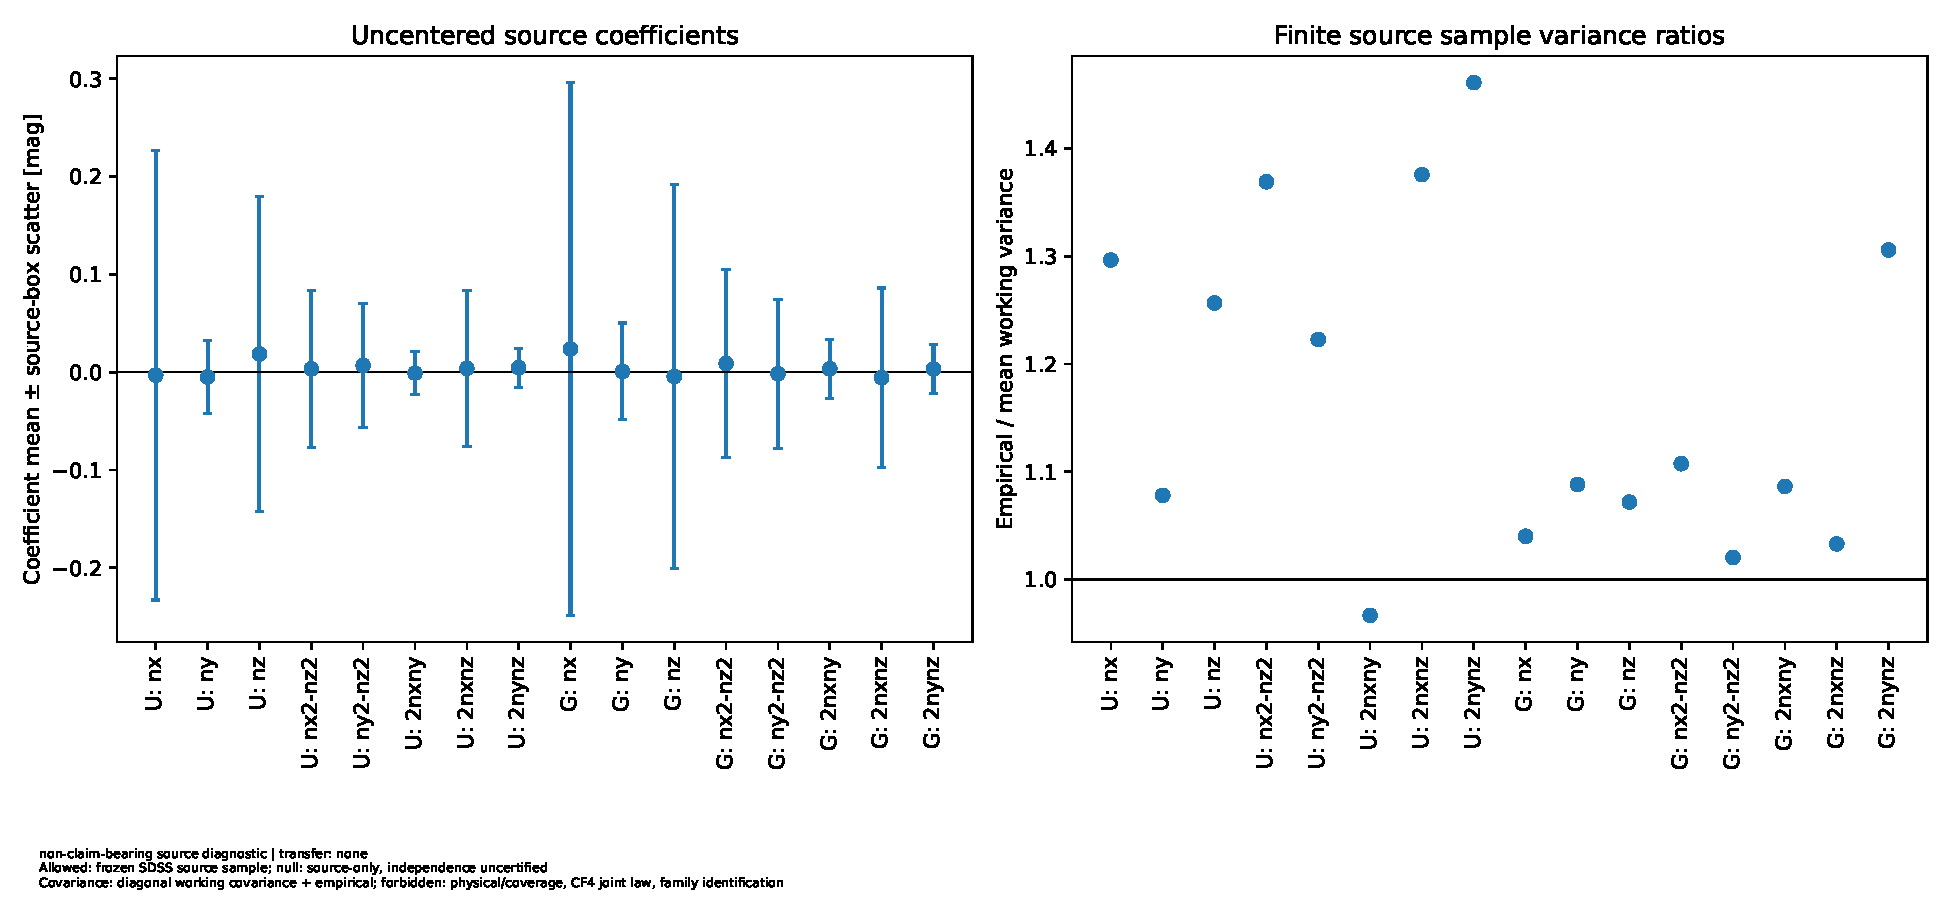
\includegraphics[width=\linewidth,height=.71\textheight,keepaspectratio]{figures/f085_external.pdf}
\caption{Uncentred coefficients and variance ratios from retained error-only SDSS source realizations. True source peculiar velocity is removed in this experiment. The finite sample diagnoses the stated error law and does not supply a physical velocity or selection null.}
\label{fig:f085}
\end{figure}
\clearpage
\begin{figure}[p]
\centering
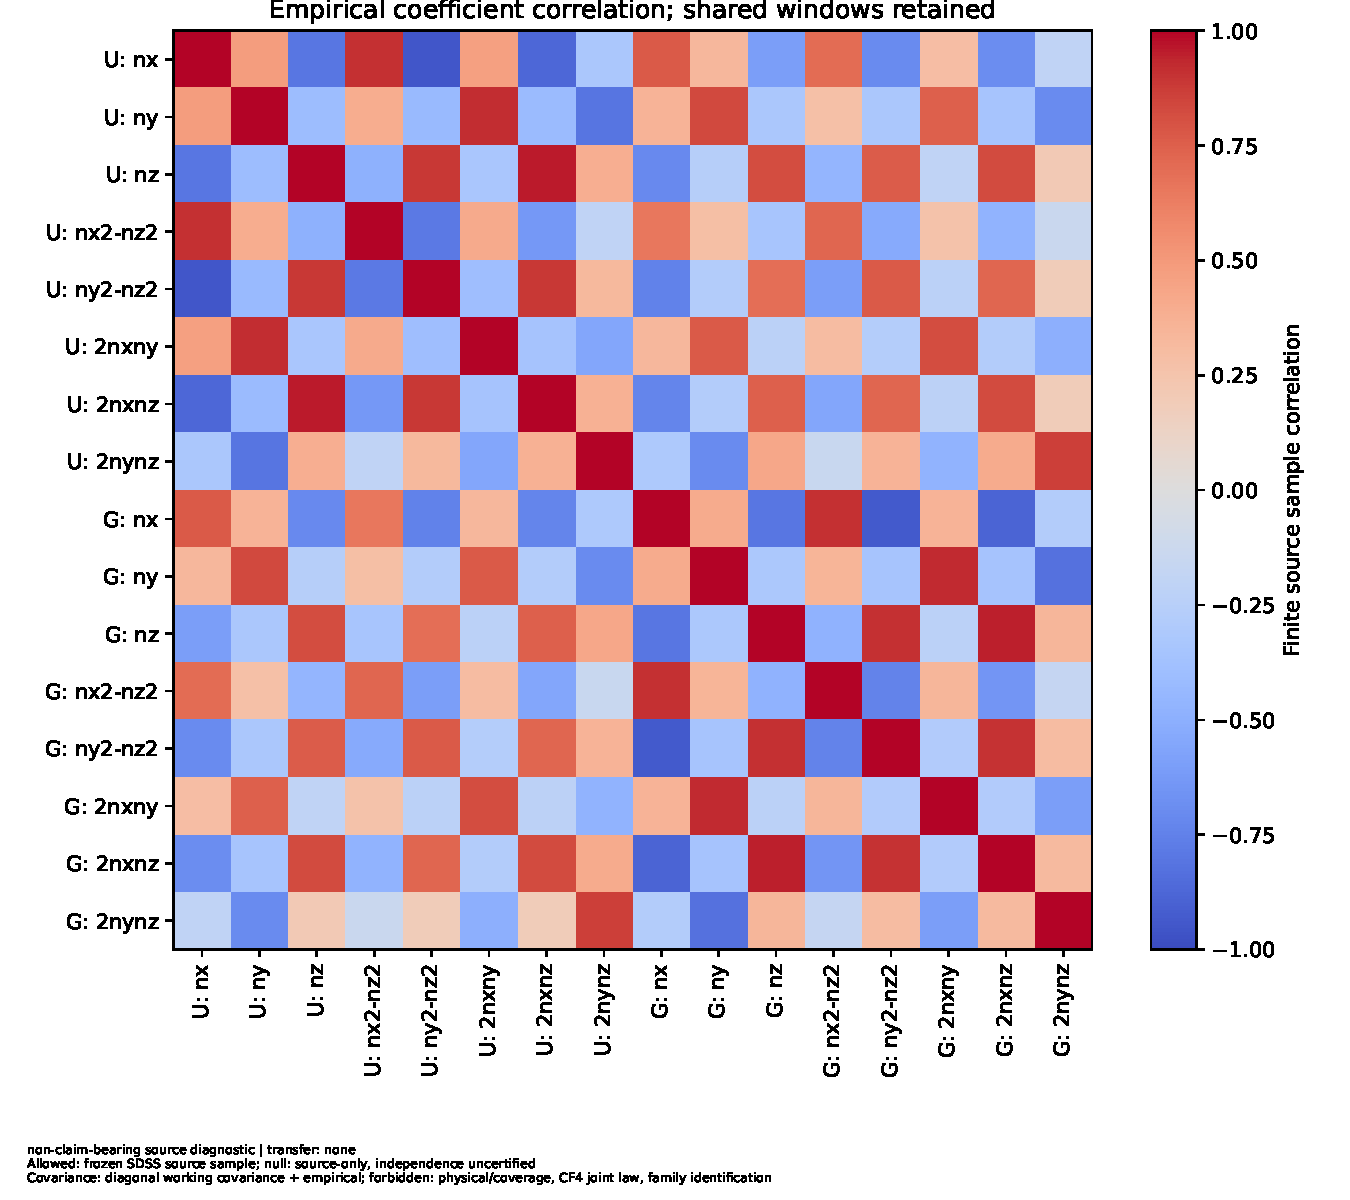
\includegraphics[width=\linewidth,height=.71\textheight,keepaspectratio]{figures/f086_external.pdf}
\caption{Empirical coefficient correlations in the same error-only source realizations. Shared angular windows remain coupled. The finite correlation matrix is descriptive and does not establish independence of the source boxes or a full physical survey covariance.}
\label{fig:f086}
\end{figure}
\clearpage
\begin{figure}[p]
\centering
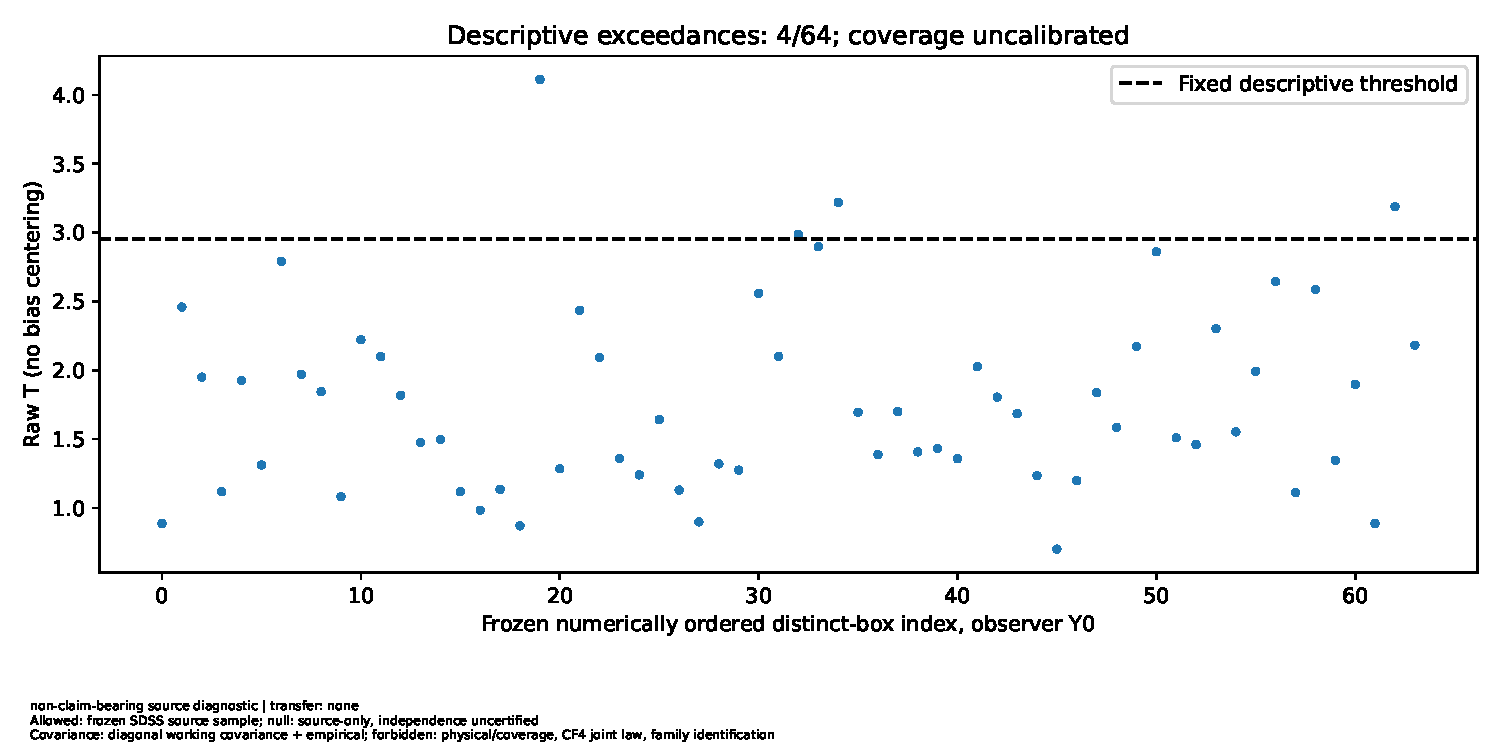
\includegraphics[width=\linewidth,height=.71\textheight,keepaspectratio]{figures/f087_external.pdf}
\caption{Raw descriptive quadratics for the retained error-only source realizations. The fixed threshold is not a calibrated physical acceptance region. Exceedance counts and uncentred bias are retained without converting them into survey coverage.}
\label{fig:f087}
\end{figure}
\clearpage
\begin{figure}[p]
\centering
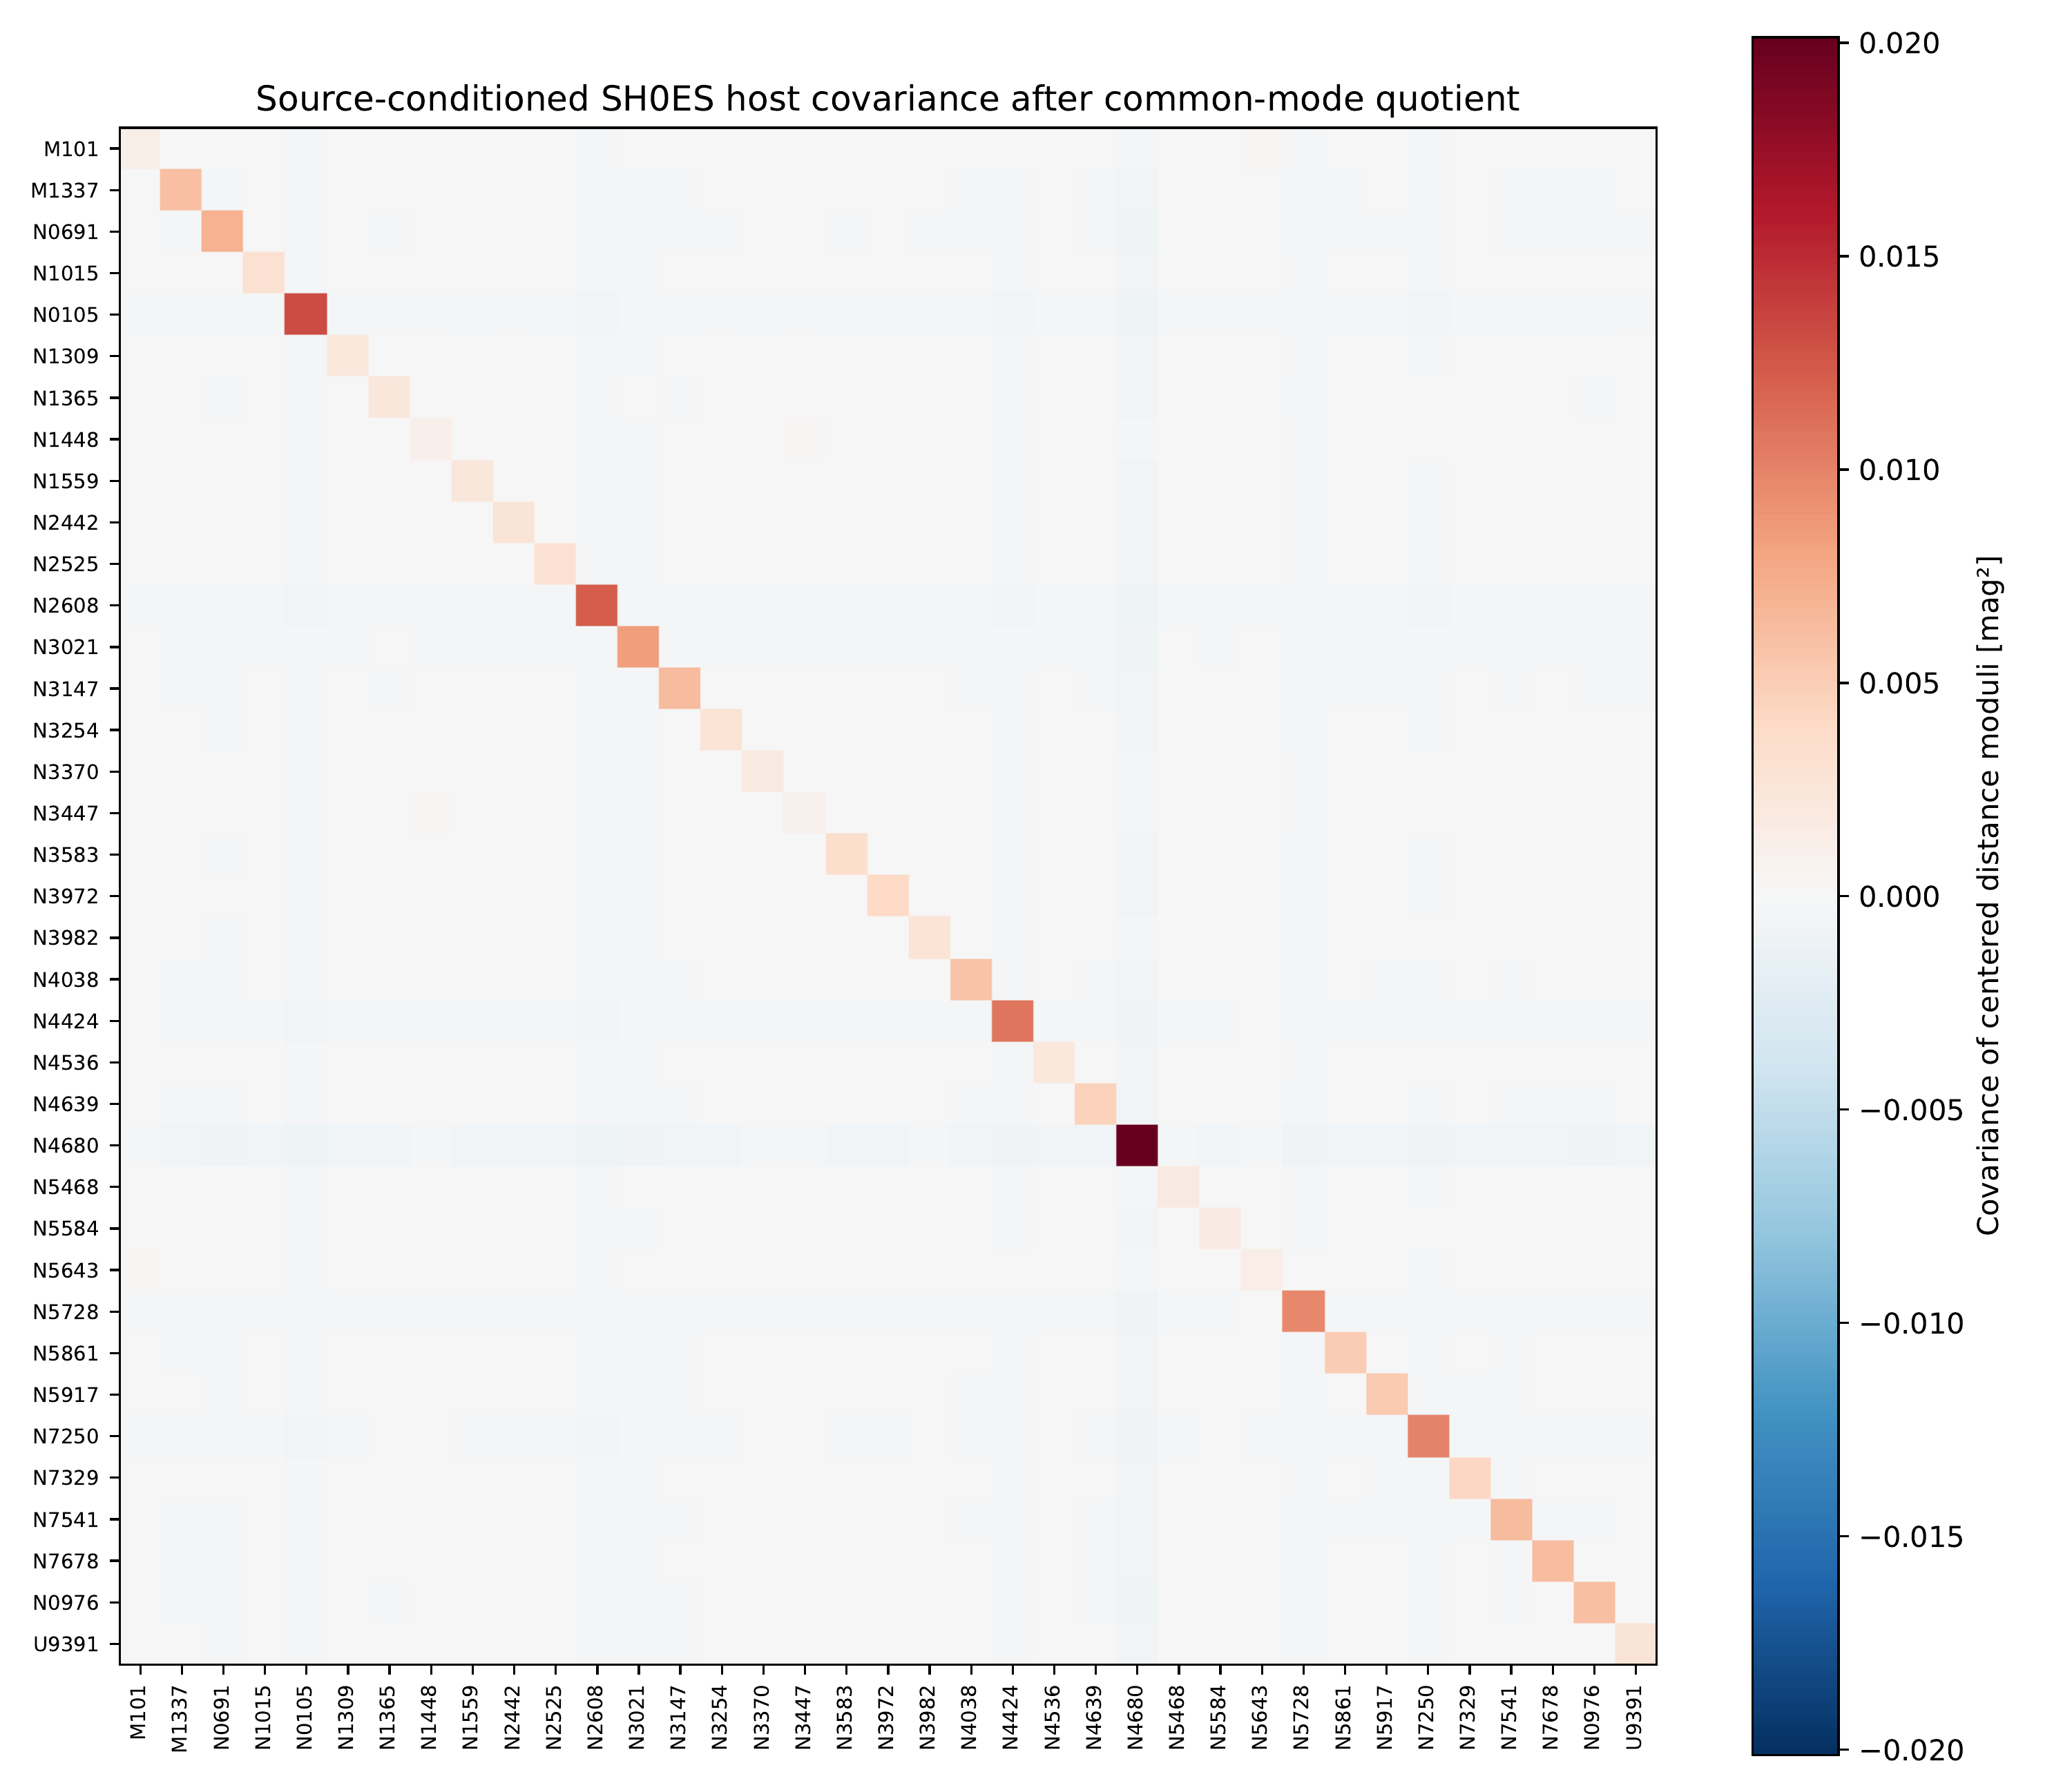
\includegraphics[width=\linewidth,height=.71\textheight,keepaspectratio]{figures/f088_external.png}
\caption{Source-conditioned SH0ES host covariance after the common-mode quotient. The Gaussian ladder reproduction is a source-model check, not a new Hubble-constant measurement. The covariance is not a joint Pantheon+--Cosmicflows source law.}
\label{fig:f088}
\end{figure}
\clearpage
\begin{figure}[p]
\centering
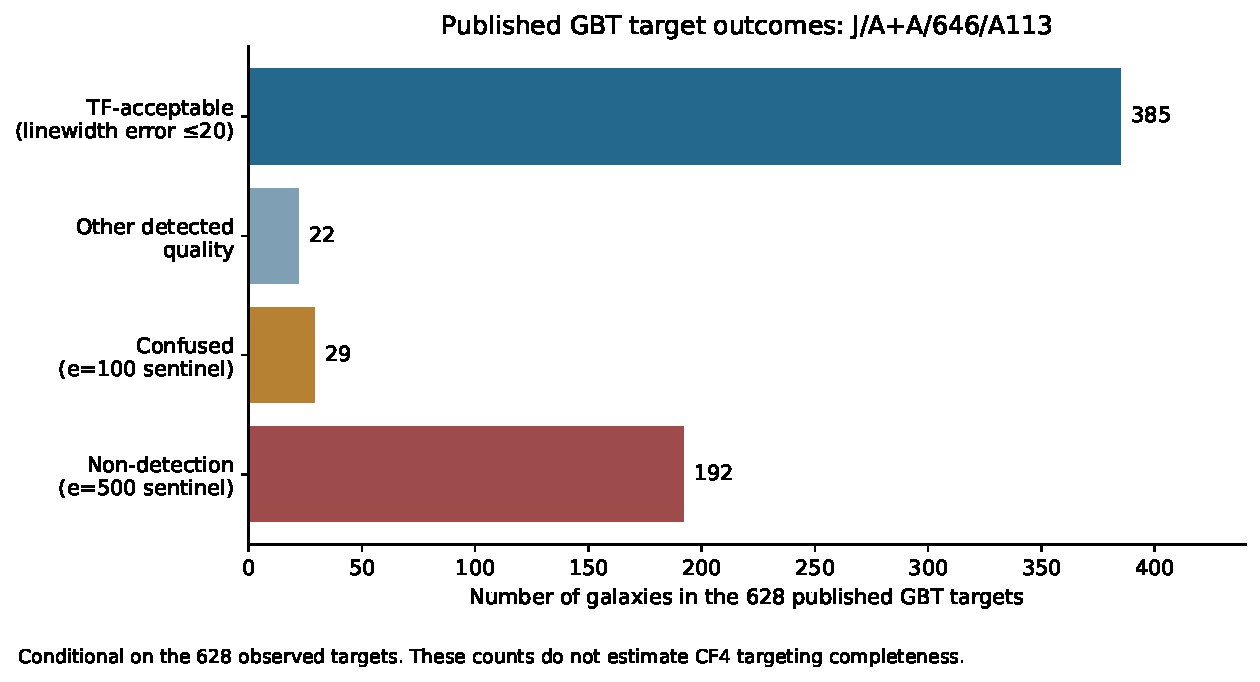
\includegraphics[width=\linewidth,height=.71\textheight,keepaspectratio]{figures/f089.pdf}
\caption{Published hydrogen-line target outcomes. Accepted, other detected, confused, and nondetected objects are distinct observational states. The counts describe the released target sample and are not interchangeable with a later crossmatched distance-bearing cohort.}
\label{fig:f089}
\end{figure}
\clearpage
\begin{figure}[p]
\centering
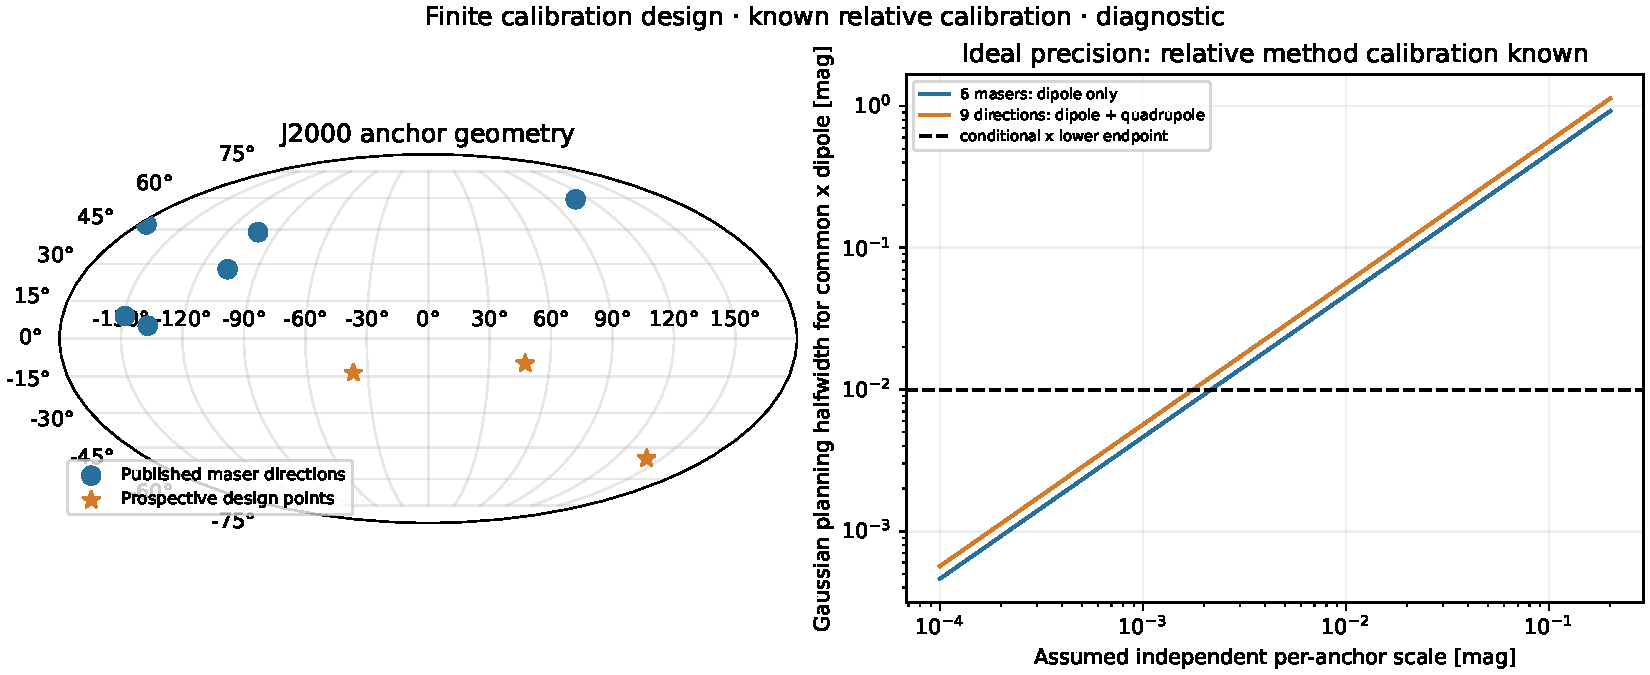
\includegraphics[width=\linewidth,height=.71\textheight,keepaspectratio]{figures/f090_external.pdf}
\caption{Maser-anchor sky geometry and hypothetical precision in six dipole-calibration directions versus nine dipole-plus-quadrupole directions. The source positions determine the geometric design. The precision curves require the stated assumed anchor uncertainties and response model; they are not measured calibration precision or an absolute shear constraint.}
\label{fig:f090}
\end{figure}
\clearpage
\begin{figure}[p]
\centering
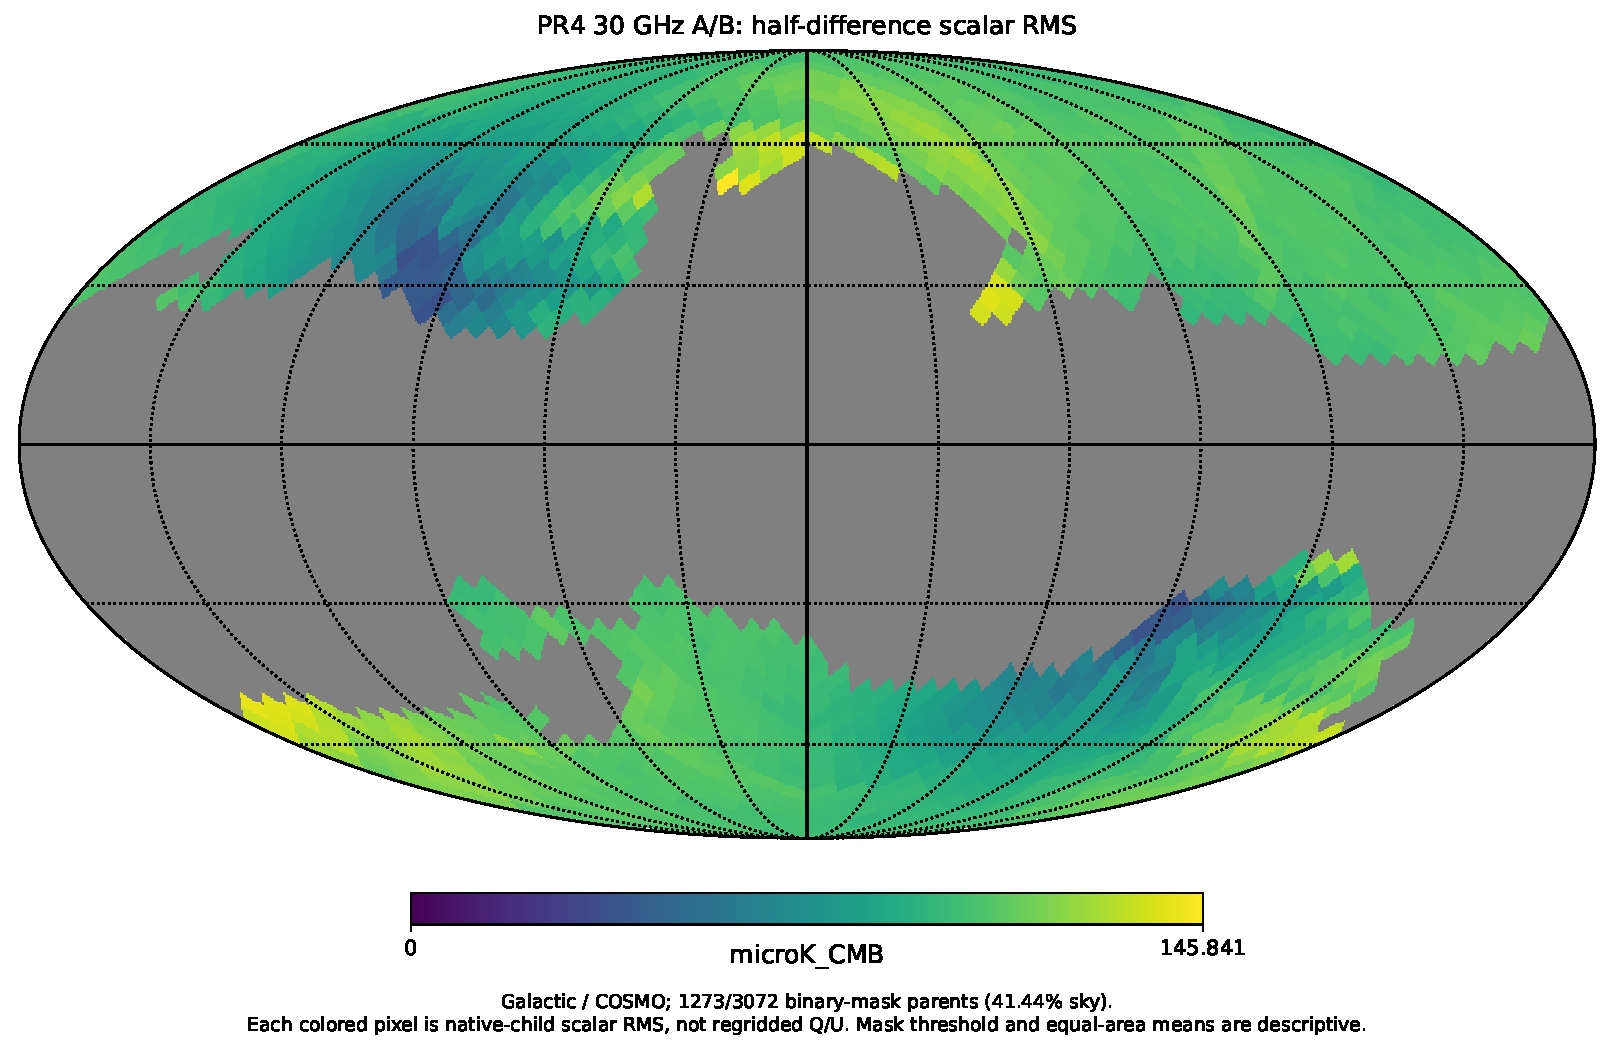
\includegraphics[width=\linewidth,height=.71\textheight,keepaspectratio]{figures/f091.pdf}
\caption{Scalar half-difference RMS for the retained Planck PR4 30-GHz pair. Each displayed cell summarizes original child pixels rather than a downgraded polarization field. Masking and component correlations remain; this is not a noise-fraction map or a calibrated anisotropy test.}
\label{fig:f091}
\end{figure}
\clearpage
\begin{figure}[p]
\centering
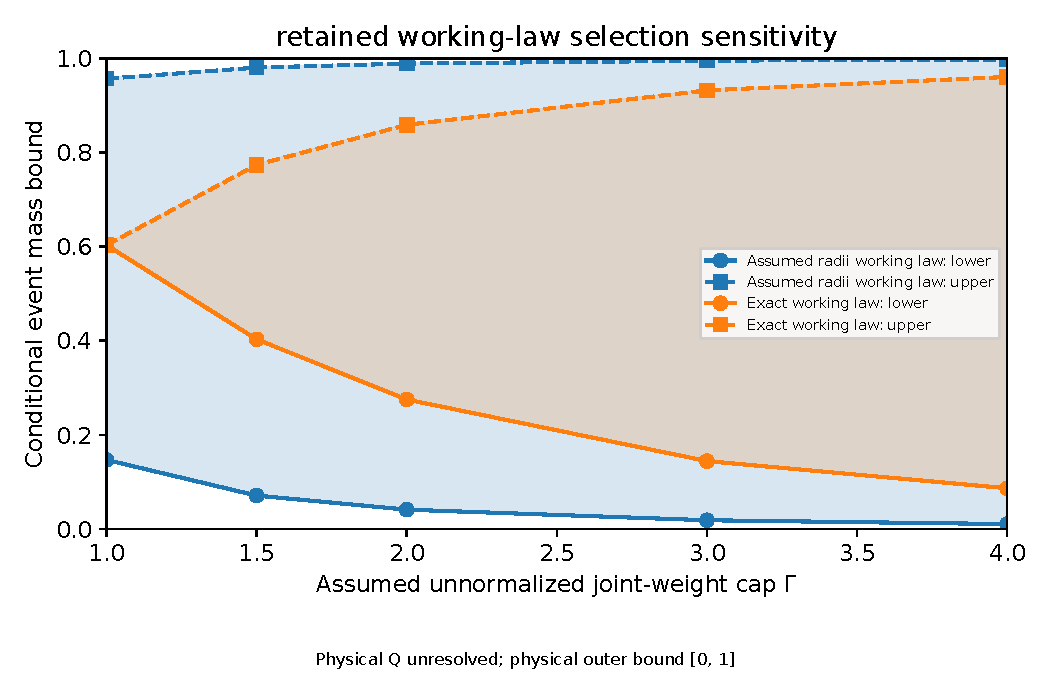
\includegraphics[width=\linewidth,height=.71\textheight,keepaspectratio]{figures/f092_external.pdf}
\caption{Selection sensitivity of the retained coupled finite measure, with exact or assumed-radius event bounds shown separately. The physical selection law is unqualified. Empirical conditional event mass is not a physical posterior or a null probability.}
\label{fig:f092}
\end{figure}
\clearpage
\begin{figure}[p]
\centering
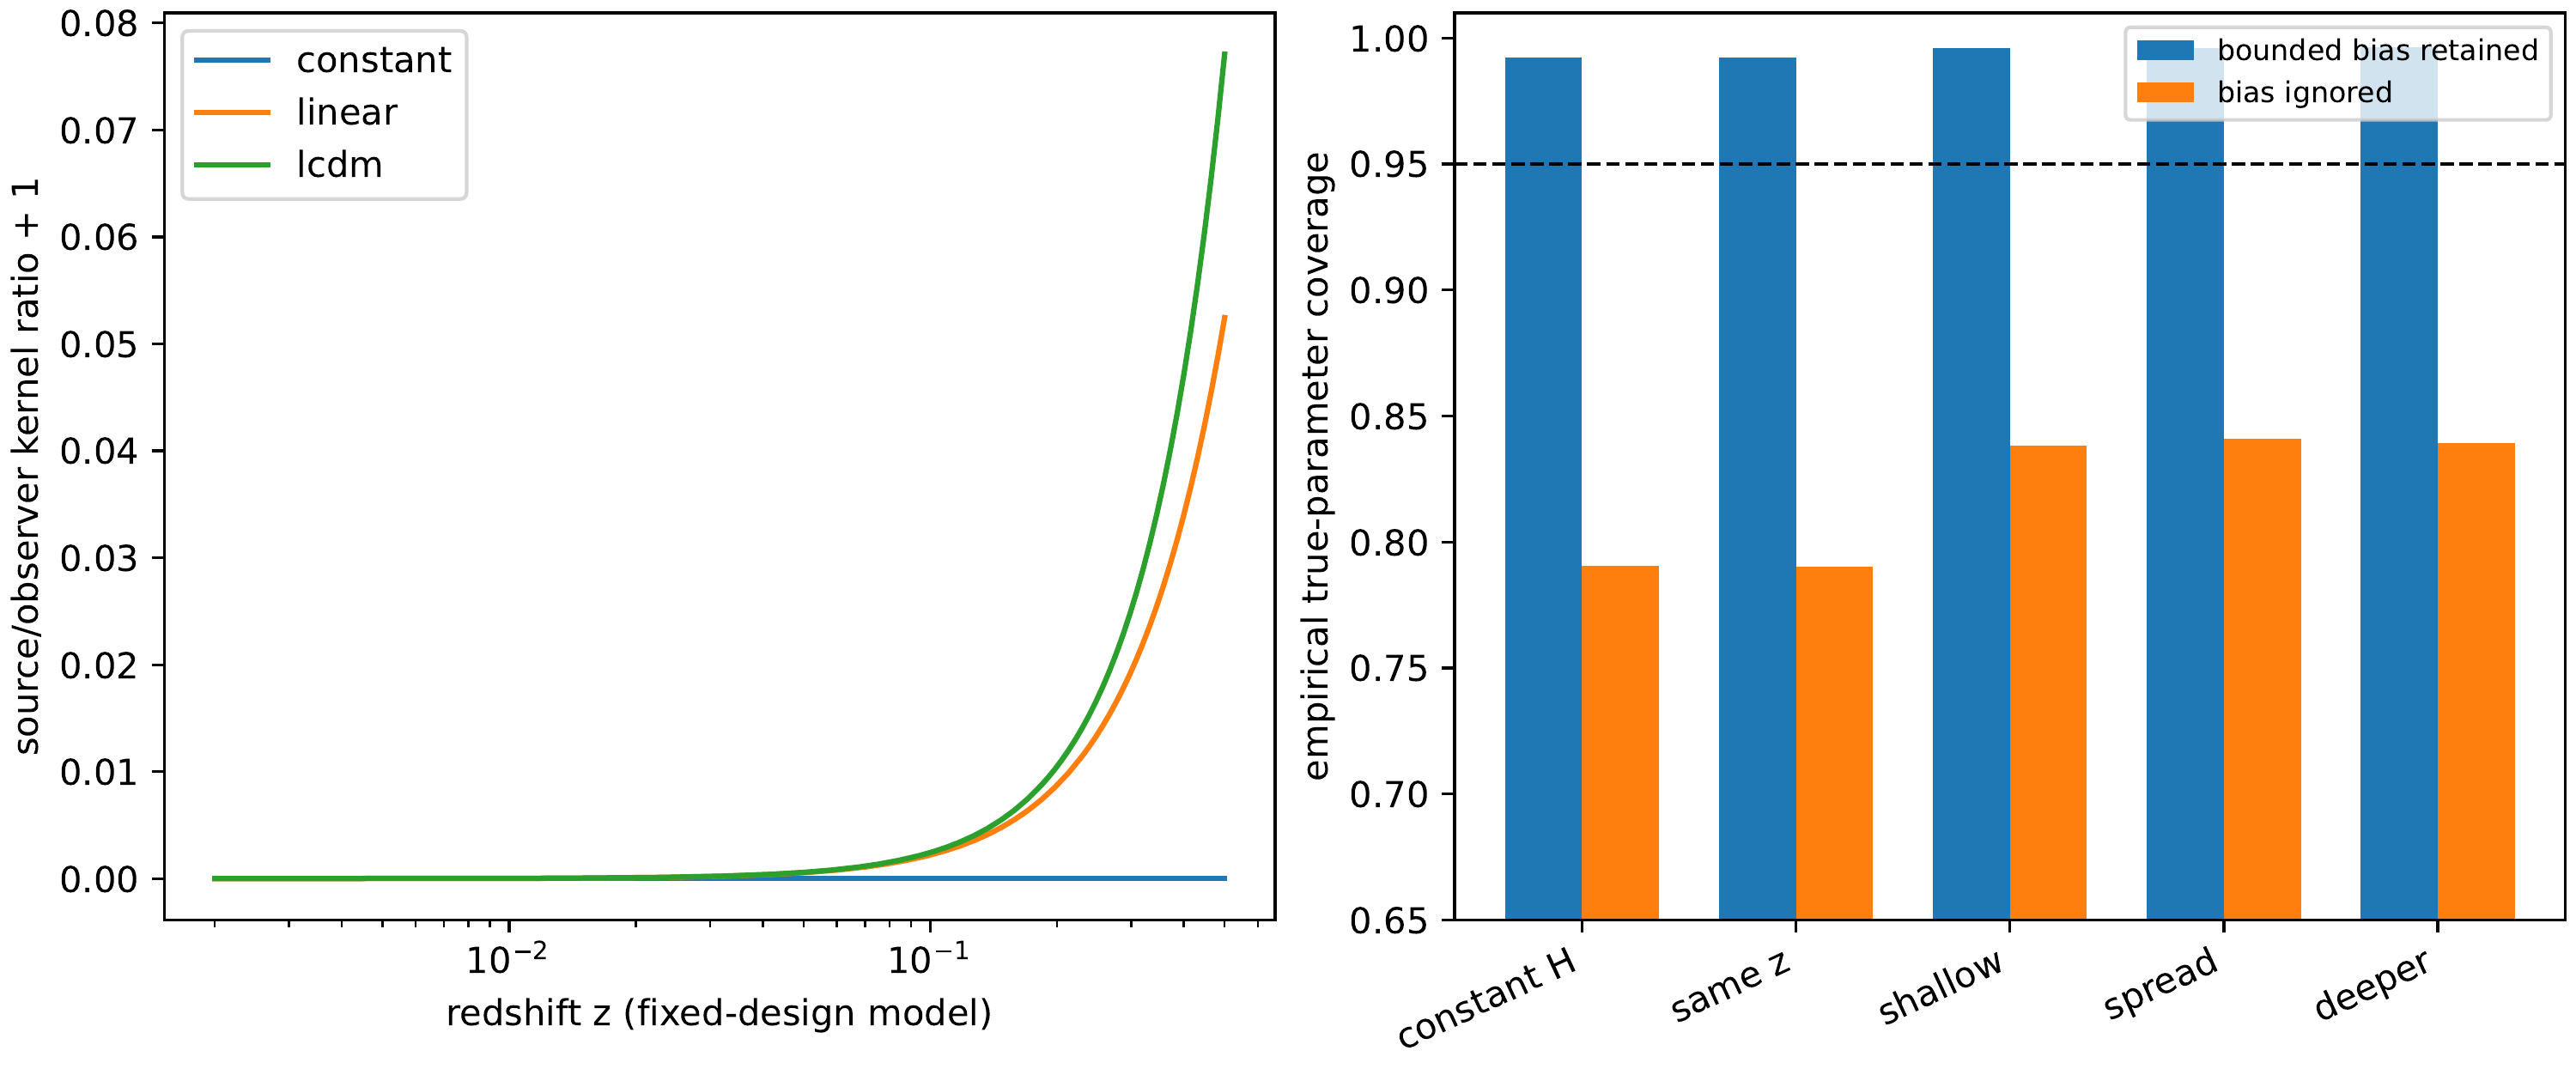
\includegraphics[width=\linewidth,height=.71\textheight,keepaspectratio]{figures/f093_external.png}
\caption{Synthetic fixed-design response and coverage controls for tensor inference. The response ratios and coverage frequencies concern the explicitly generated model. They are not observational constraints or evidence of physical source-law validity.}
\label{fig:f093}
\end{figure}
\clearpage
\begin{figure}[p]
\centering
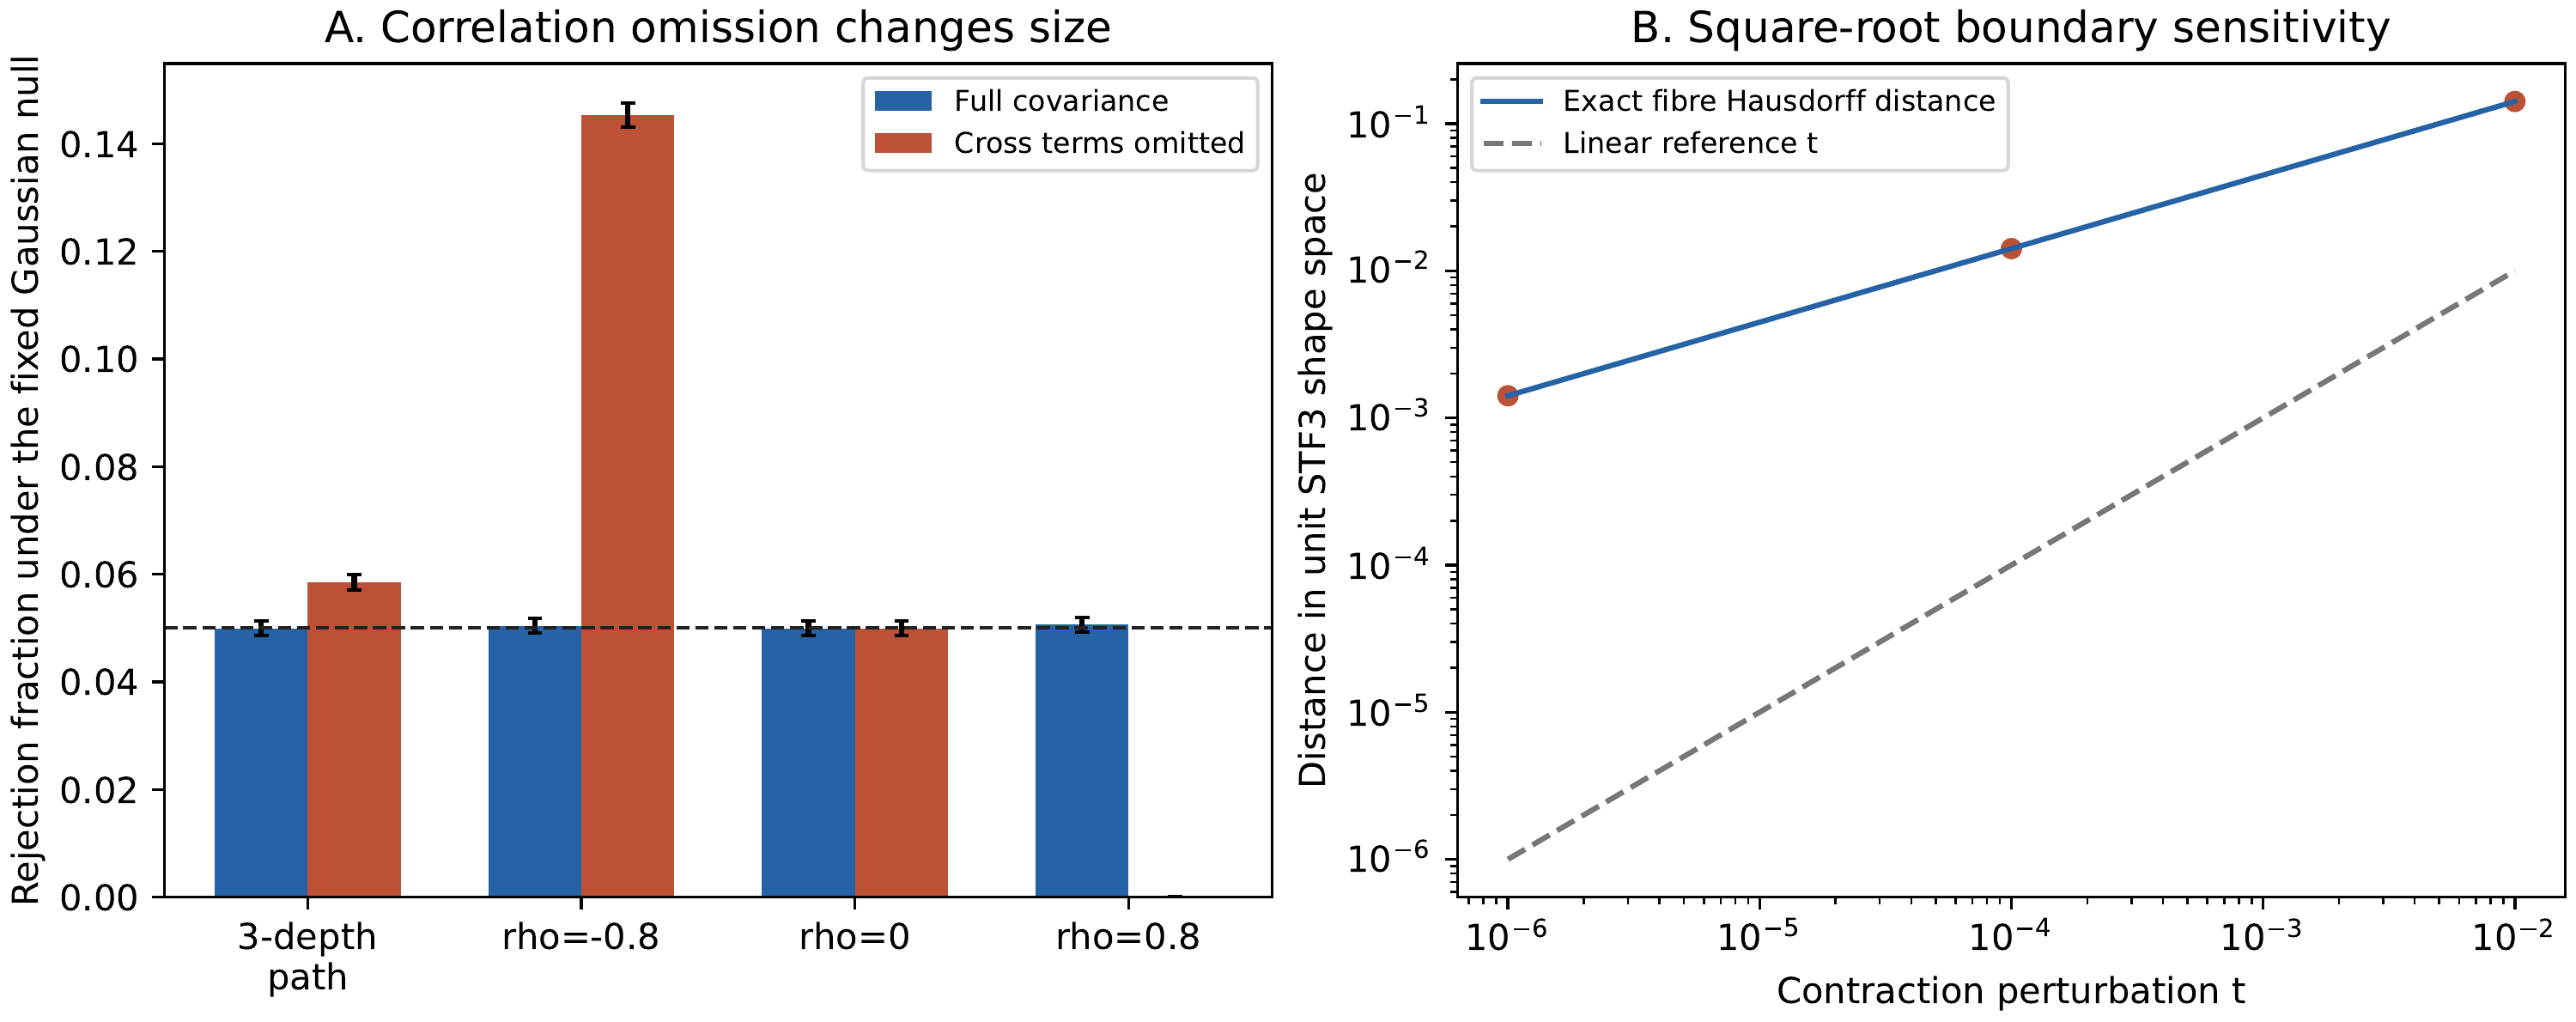
\includegraphics[width=\linewidth,height=.71\textheight,keepaspectratio]{figures/f094_external.png}
\caption{Synthetic controls for omitted covariance, nonlinear boundaries, and joint tensor images. Dropping cross terms changes error rates, and square-root boundaries invalidate an unqualified linear approximation. These controls motivate retention of the full state and support; they are not additional observations.}
\label{fig:f094}
\end{figure}
\clearpage
\begin{figure}[p]
\centering
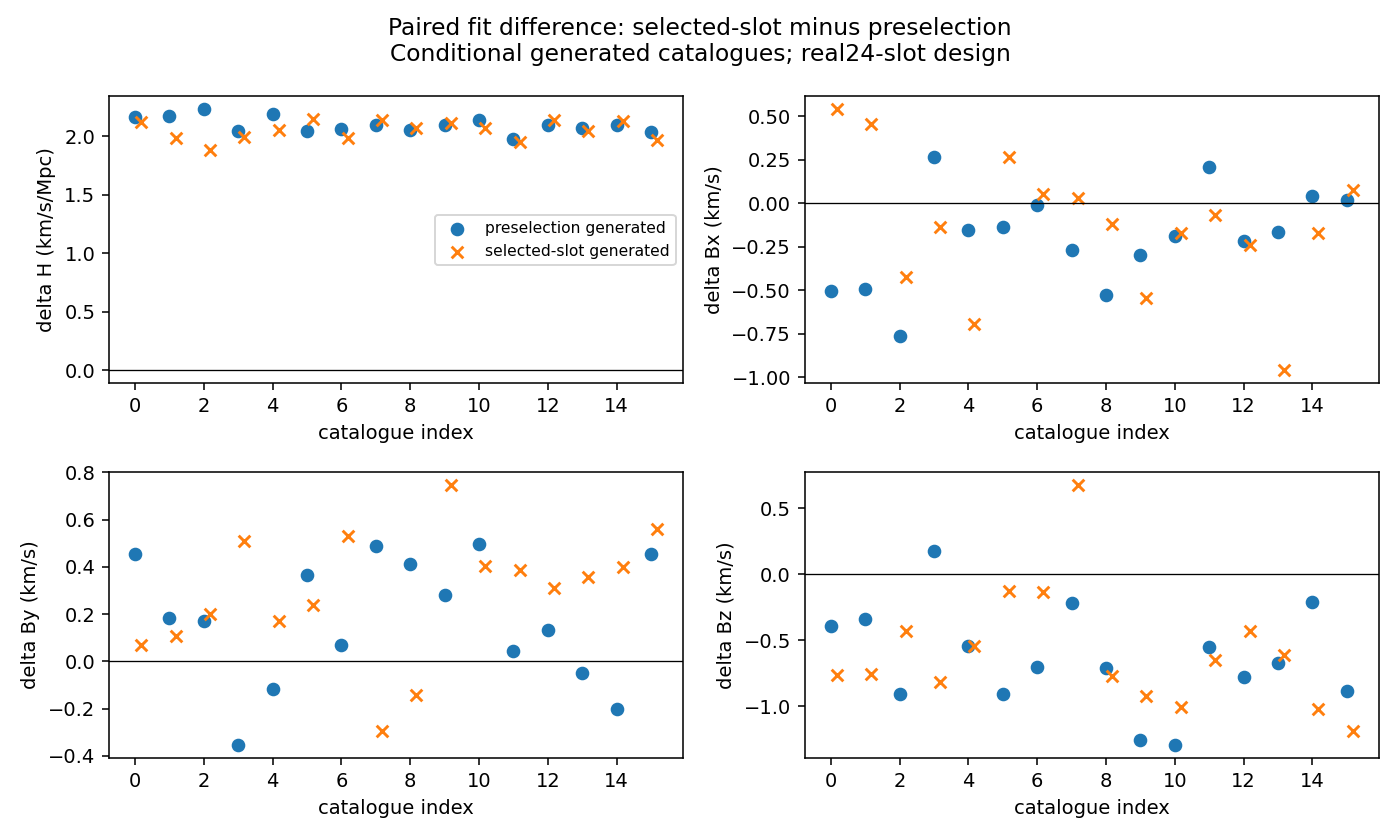
\includegraphics[width=\linewidth,height=.71\textheight,keepaspectratio]{figures/f096.png}
\caption{Paired generated Cosmicflows catalogues under distinct declared source laws. Differences between laws are kept separate from within-law sampling variation. This preview does not identify the actual catalogue selection or physical uncertainty model.}
\label{fig:f096}
\end{figure}
\clearpage
\begin{figure}[p]
\centering
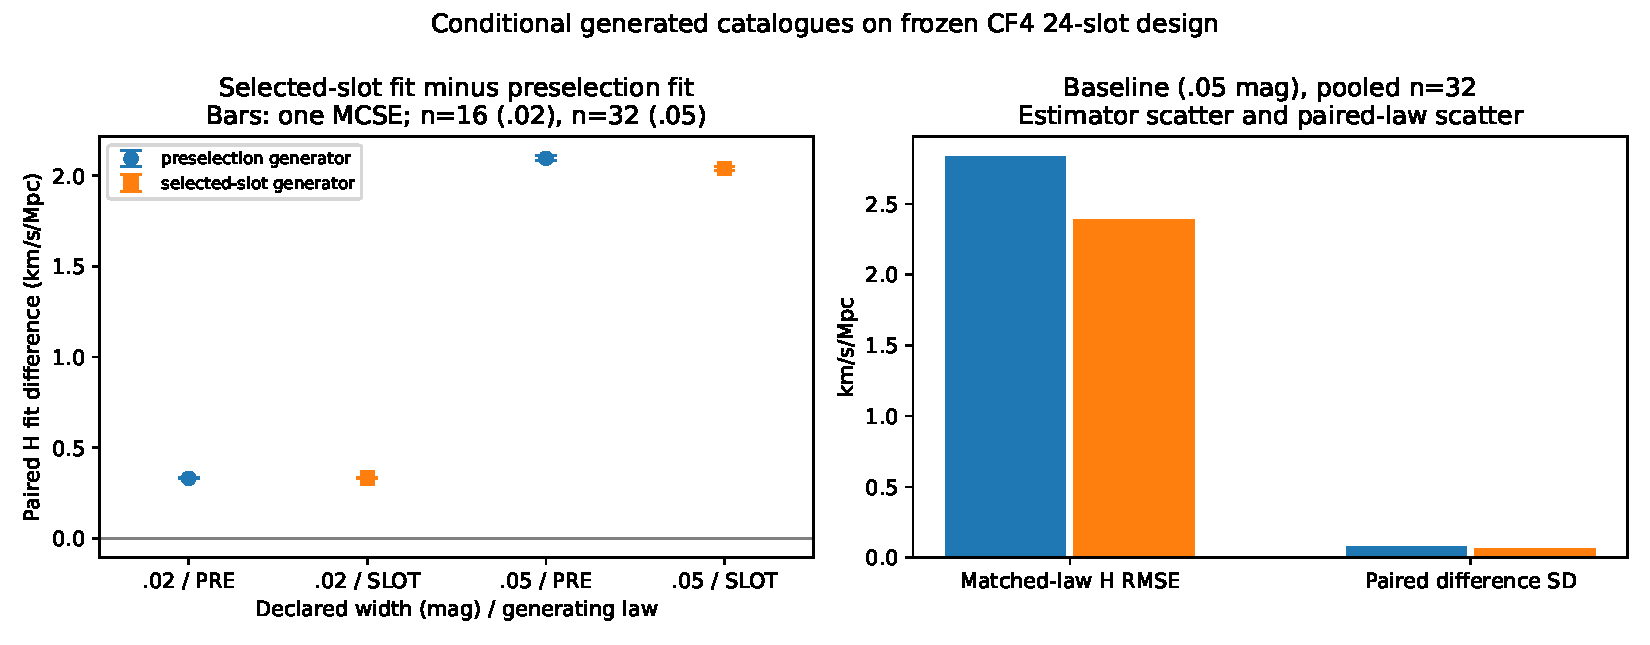
\includegraphics[width=\linewidth,height=.71\textheight,keepaspectratio]{figures/f097.pdf}
\caption{Conditional generated-catalogue precision on a frozen Cosmicflows design. Preselection and selected-slot generators are different experiments. Increasing replication narrows simulation scatter without validating either generator as the observed source law.}
\label{fig:f097}
\end{figure}
\clearpage
\begin{figure}[p]
\centering
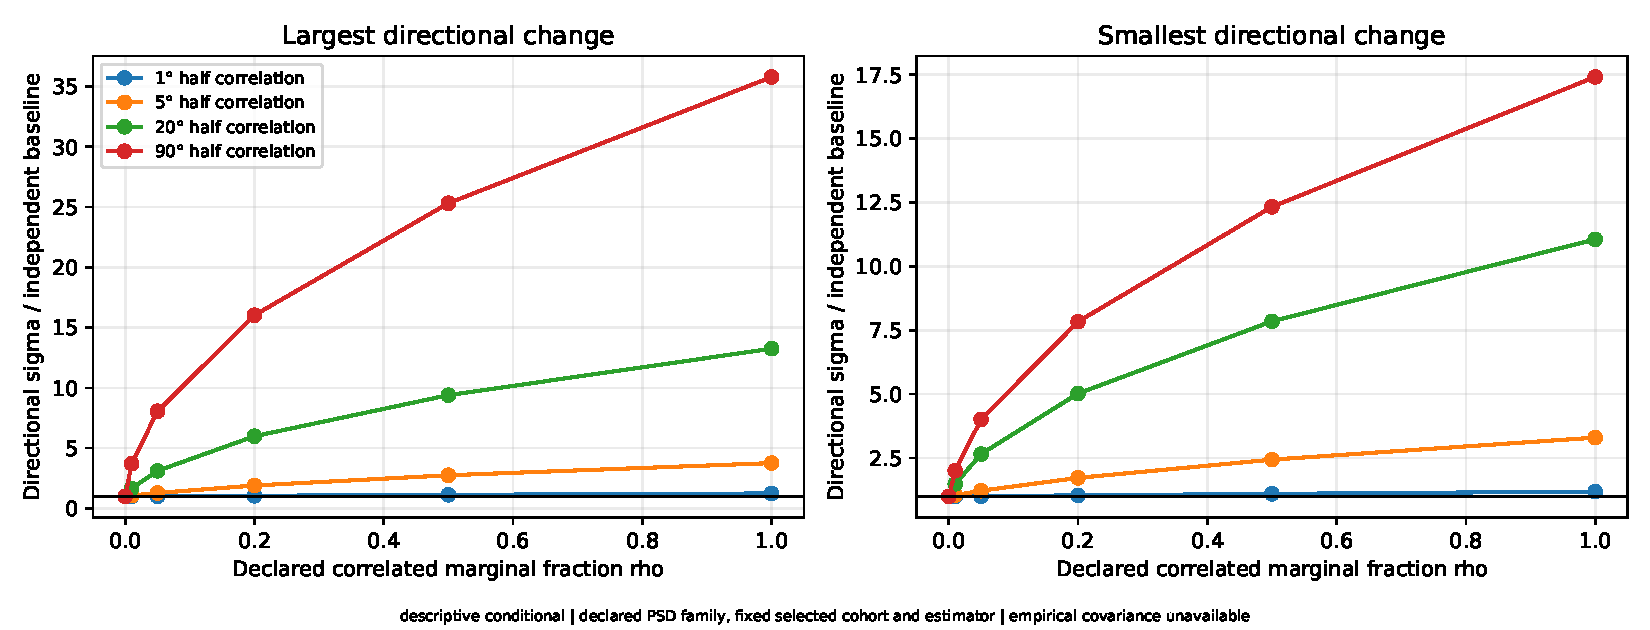
\includegraphics[width=\linewidth,height=.71\textheight,keepaspectratio]{figures/f098_external.pdf}
\caption{Angular-correlation sensitivity in a fixed Gaia source design. The specified correlation families are scenarios. They show dependence of inference on covariance assumptions rather than measuring the actual sky correlation law.}
\label{fig:f098}
\end{figure}
\clearpage
\begin{figure}[p]
\centering
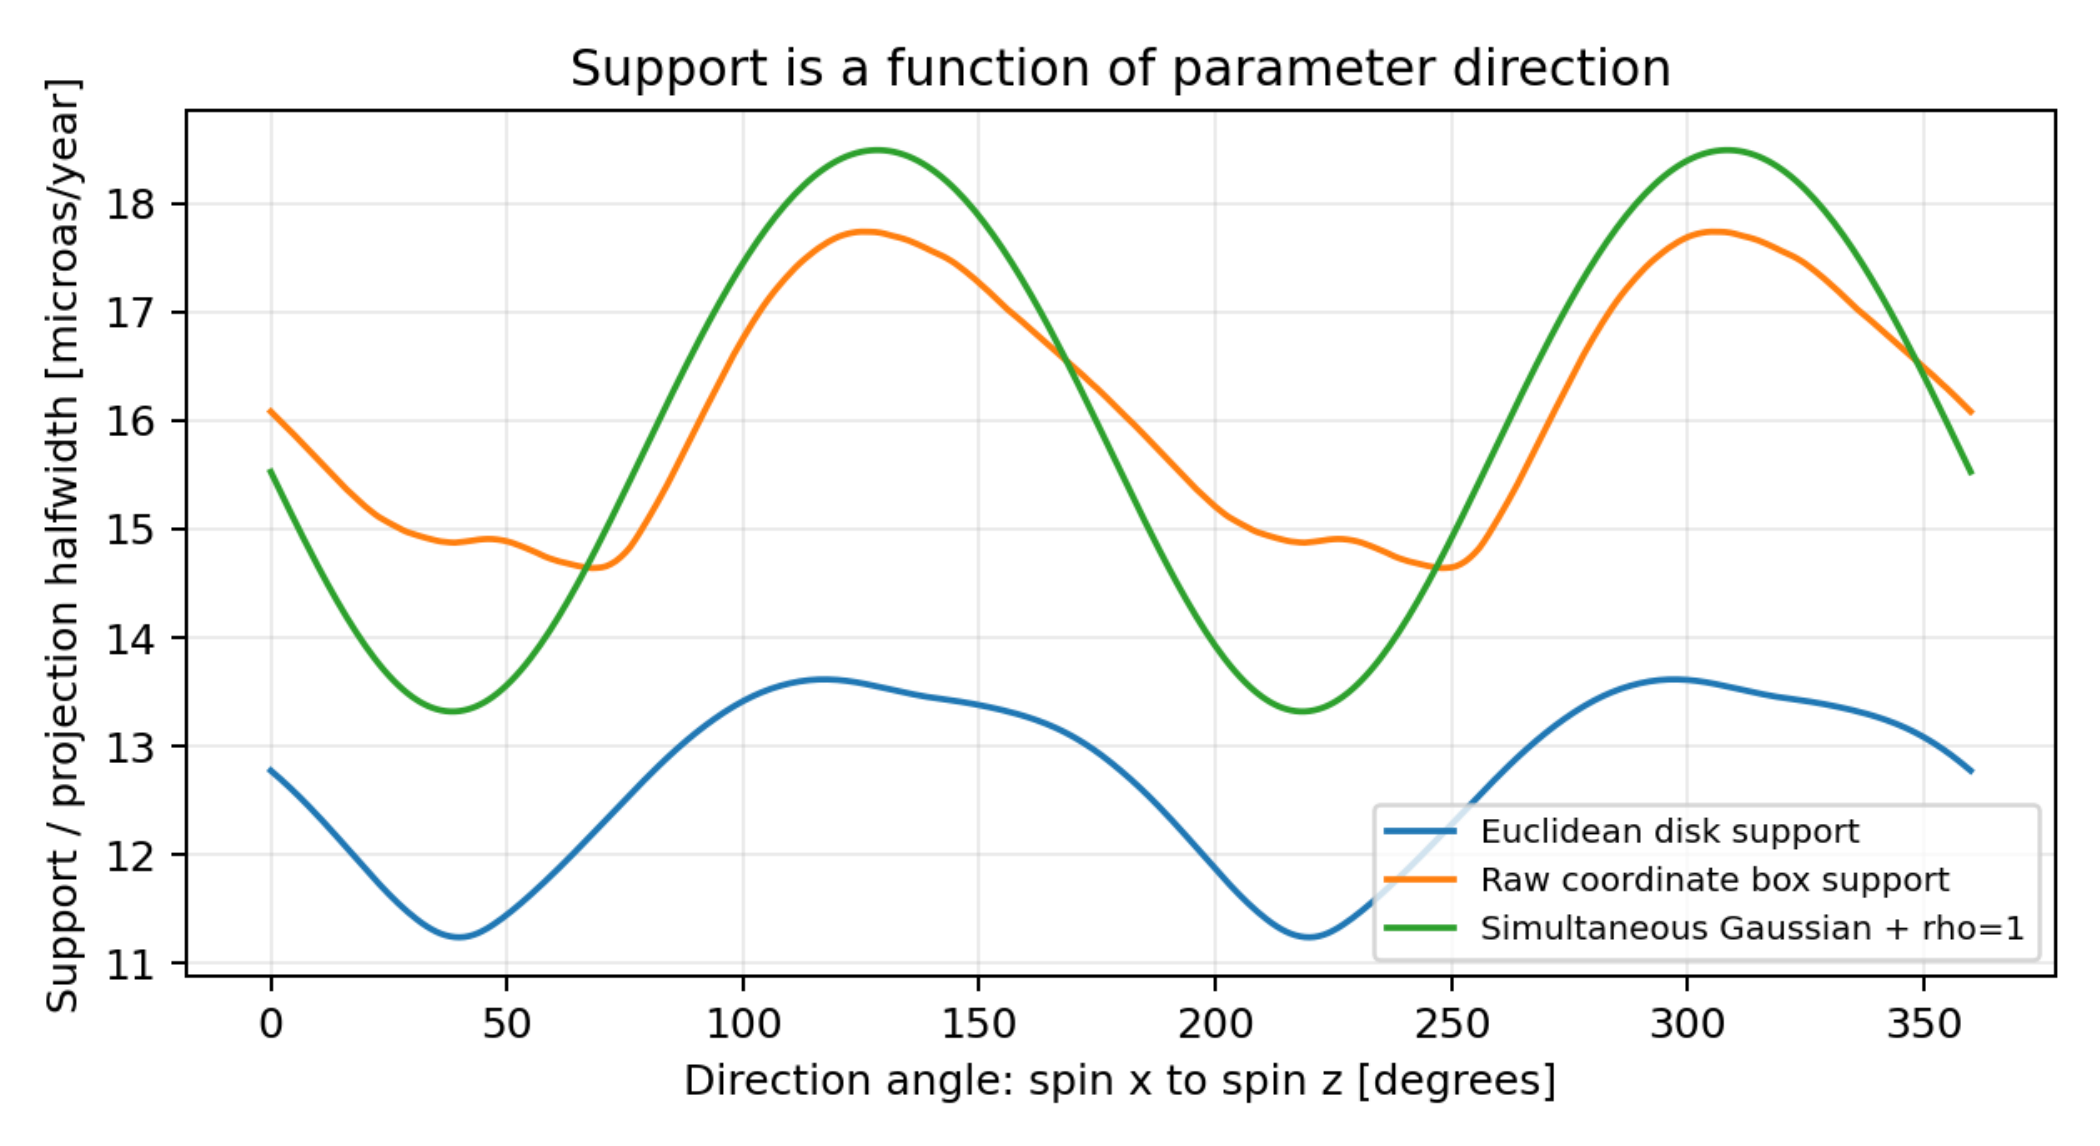
\includegraphics[width=\linewidth,height=.71\textheight,keepaspectratio]{figures/f099_external.png}
\caption{Directional support of a fixed astrometric proxy experiment. The complete operator and state define the plotted support. This geometry does not establish physical Gaia coverage, a matter-following source response, or a probability within the support.}
\label{fig:f099}
\end{figure}
\clearpage
\begin{figure}[p]
\centering
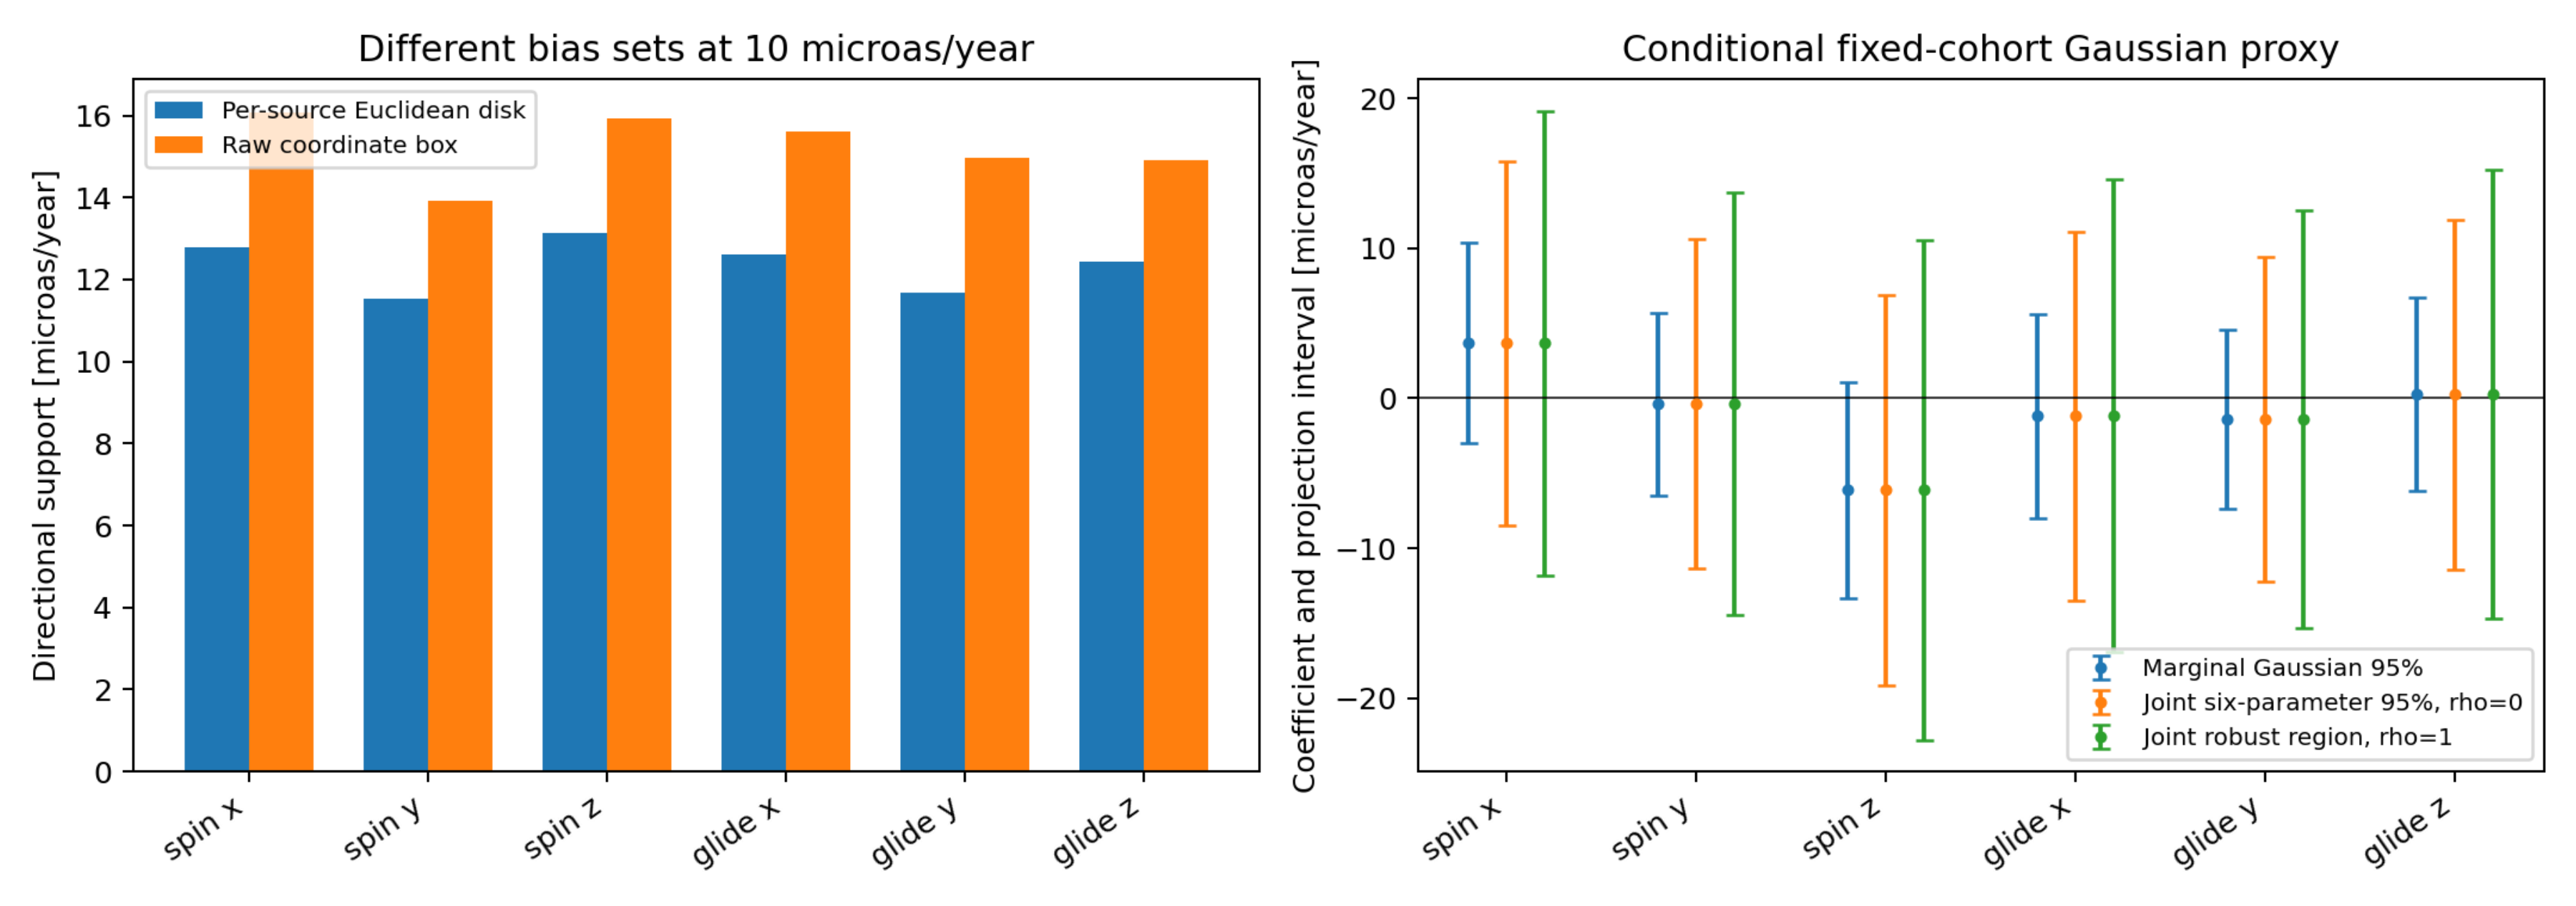
\includegraphics[width=\linewidth,height=.71\textheight,keepaspectratio]{figures/f100_external.png}
\caption{Euclidean-disk and coordinate-box bias supports for the fixed astrometric proxy design, together with marginal and joint Gaussian proxy intervals. The support geometry changes the allowed image even at the same coordinate scale. The assumed bias sets and Gaussian law do not establish physical Gaia uncertainty or population coverage.}
\label{fig:f100}
\end{figure}
\clearpage
\begin{figure}[p]
\centering
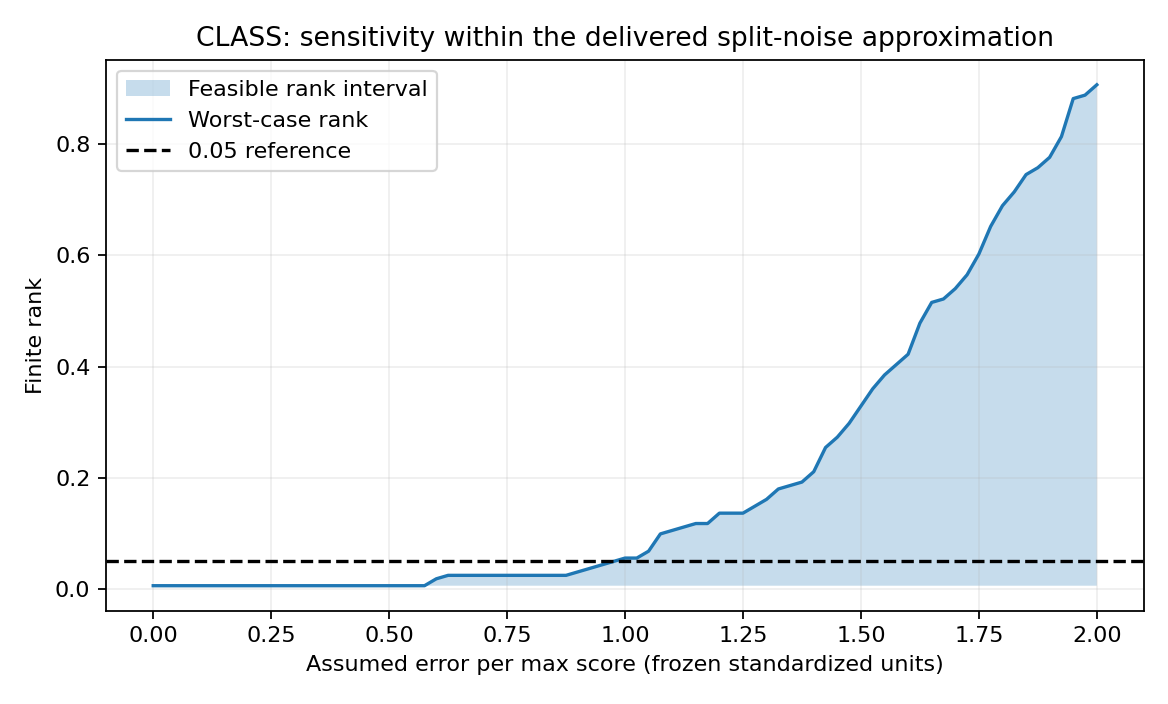
\includegraphics[width=\linewidth,height=.71\textheight,keepaspectratio]{figures/f101.png}
\caption{Finite tail-rank sensitivity for the CLASS split-noise comparison with 160 reference scores. The interval widens as an assumed error allowance is applied to the observed and reference scores. This allowance is not a measured physical systematic bound. Finite rank arithmetic does not establish exchangeability or turn the split-noise approximation into a physical null law.}
\label{fig:f101}
\end{figure}
\clearpage
\begin{figure}[p]
\centering
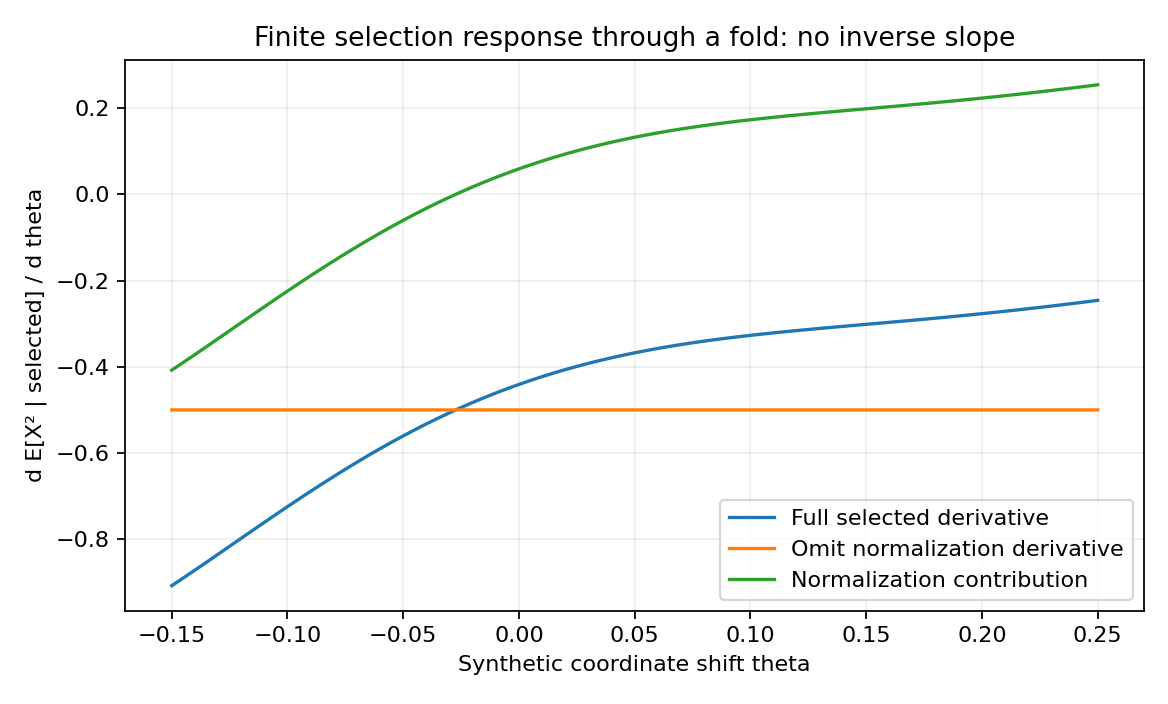
\includegraphics[width=\linewidth,height=.71\textheight,keepaspectratio]{figures/f102.png}
\caption{A synthetic nonlinear selection response: X is uniform on [-1,1], the latent quantity is X squared plus theta, and Gaussian measurement noise has standard deviation 0.1; observations are selected between -0.1 and 0.4. The derivative of the selected mean of X squared includes the derivative of the selection normalization. The curves concern this dimensionless generated model, not cross-validation or an observed catalogue fit.}
\label{fig:f102}
\end{figure}
\clearpage
\begin{figure}[p]
\centering
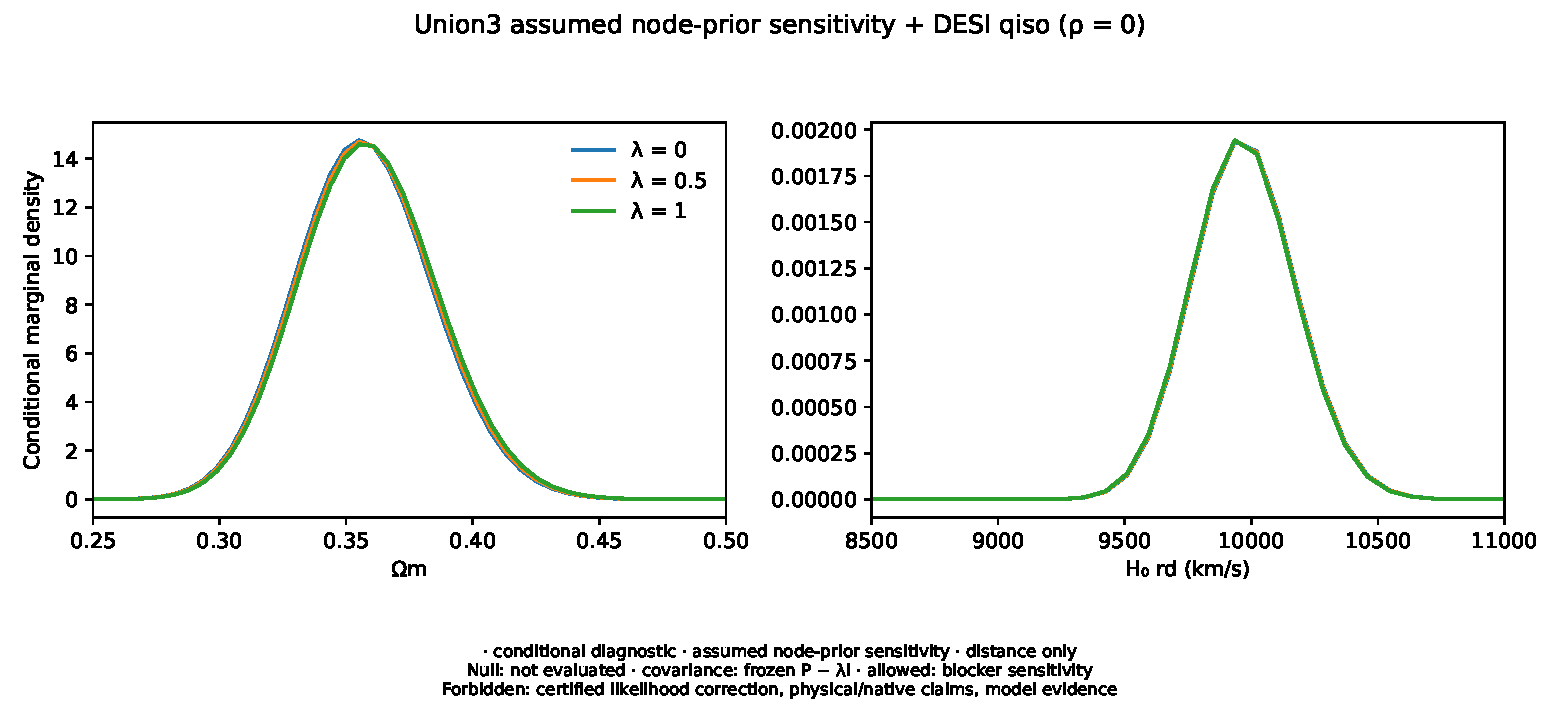
\includegraphics[width=\linewidth,height=.71\textheight,keepaspectratio]{figures/f103_external.pdf}
\caption{Union3 and DESI distance sensitivity to removal of an assumed Gaussian distance-node prior, with removal fractions zero, one-half, and one and cross-source correlation fixed to zero. The scenario marginals depend on that assumed prior and source precision. The exact released-matrix relation to the published prior and public code remains unresolved, so these curves are not a certified correction to the released likelihood or a cross-scenario evidence comparison.}
\label{fig:f103}
\end{figure}
\clearpage
\begin{figure}[p]
\centering
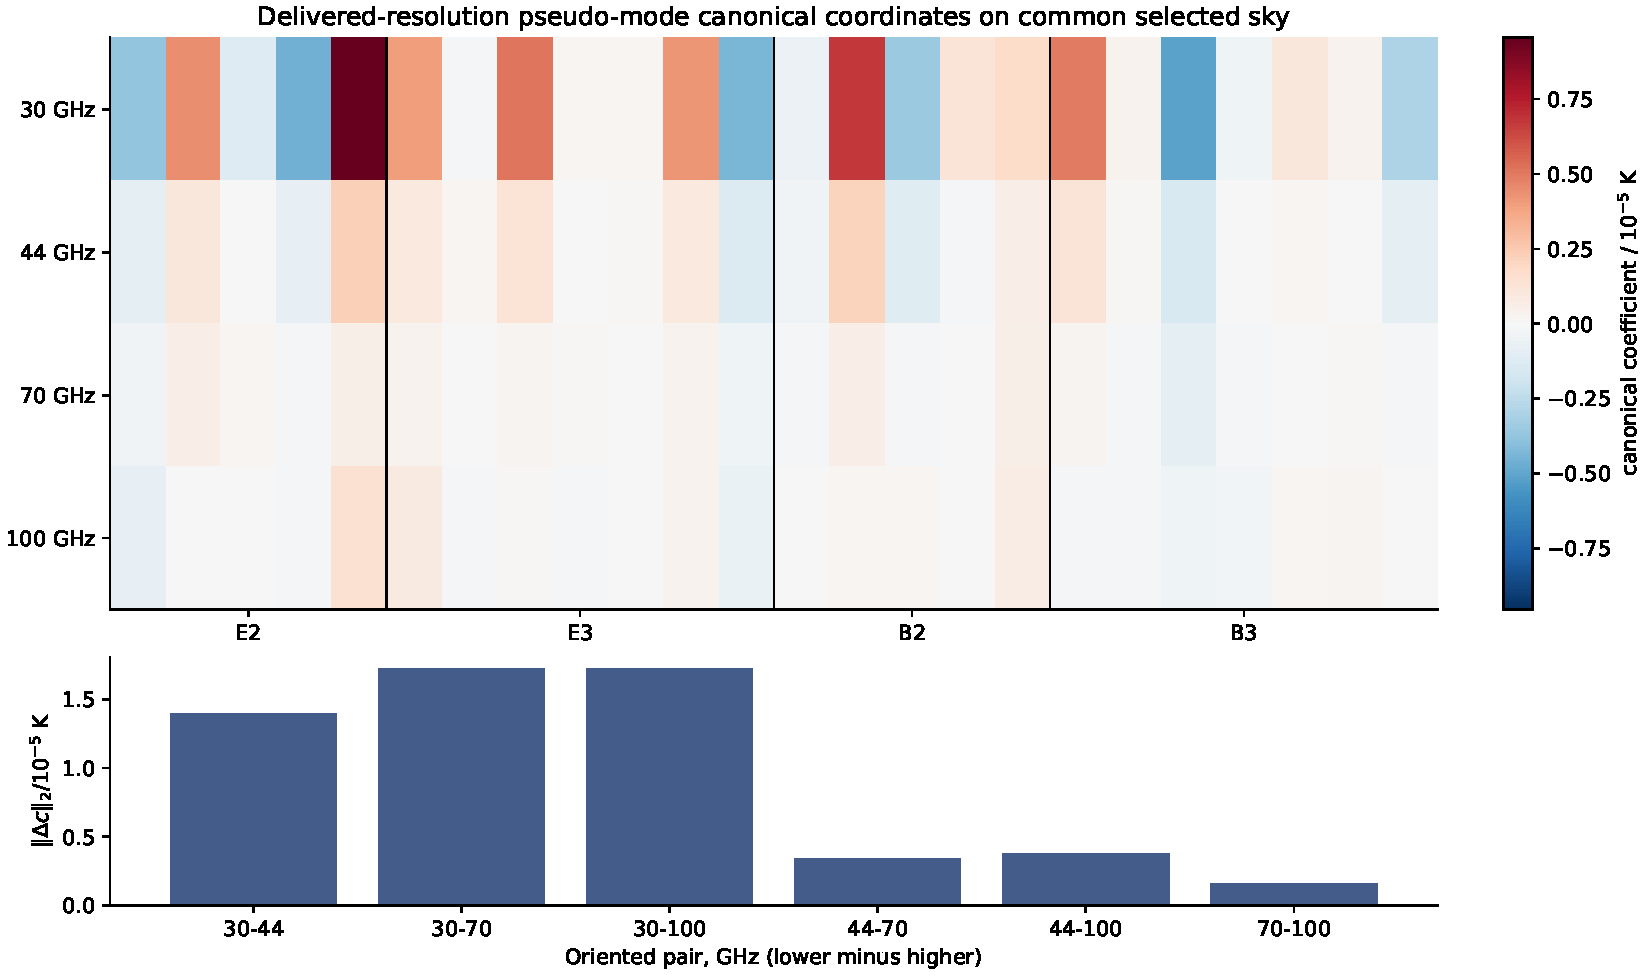
\includegraphics[width=\linewidth,height=.71\textheight,keepaspectratio]{figures/f104_external.pdf}
\caption{Complete quadrupole and octupole E/B pseudo-harmonic coordinates at four delivered frequencies and all six full-coordinate contrast norms. A common selected sky is used without map downgrading or deconvolution. Delivered beams, foregrounds, and mask leakage remain. These descriptive tensors do not supply a physical null, a frequency-to-depth map, or a completed seven-frequency result.}
\label{fig:f104}
\end{figure}
\clearpage
}{}
\bibliographystyle{apsrev4-2}
\bibliography{references}
\end{document}
